% 사용 가능한 옵션 리스트는 아래와 같습니다.
% 'doctor - master': 박사인가 석사인가
% 'final': 최종본일 경우 추가
% 'twosides - oneside': 양면인가 단면인가
% 'krabst': 국문초록
% 'krack': 한글 감사의 글
% 'asym': 홀수쪽과 짝수쪽에 제본 여백을 5mm 주고 반대쪽 여백을 5mm 줄임
%         대부분의 제본소에서는 중앙에 있는것을 선호함 (제본소 문의 바람)
%
% 예제
% \documentclass[master,final,oneside]{KUThesis}

% 기본옵션은 [doctor,twosides,draft] 입니다.  
%\documentclass[final]{KUThesis}
\documentclass[final, oneside]{KUThesis}
%\documentclass[final, krack, oneside]{KUThesis}

\usepackage[cjk]{kotex}
\usepackage{booktabs}
\usepackage[disable]{todonotes}
\newcommand{\todoTBD}[2][]{\todo[#1]{TBD #2}}
\newcommand{\todoP}[2][]{\todo[#1]{P3 #2}}
\newcommand{\todoPP}[2][]{\todo[#1]{P2 #2}}
\newcommand{\todoPPP}[2][]{\todo[#1]{P1 #2}}
\usepackage{amsthm} %for theorem
\theoremstyle{definition}
\newtheorem{definition}{Definition}[section]
\newtheorem{theorem}{Theorem}[section]
%\usepackage{algpseudocode}% http://ctan.org/pkg/algorithmicx
\usepackage{subcaption}
\usepackage{tabularx}
\usepackage{listings}
\usepackage{color,soul}
%ICSE18
\usepackage{mathtools, amsfonts, mathrsfs}
\usepackage{makecell, multirow, url}
\let\labelindent\relax
\usepackage[inline]{enumitem}
%ASE18
\usepackage{algorithm}
\usepackage[noend]{algpseudocode}
\usepackage{amsmath,amssymb}
\usepackage{balance}
%FSE19
\usepackage{pifont}
\usepackage{xcolor}
\theoremstyle{definition}
\newtheorem{example}{example}[section]

\usepackage{graphicx}
\usepackage{textcomp}
\DeclarePairedDelimiter{\ceil}{\lceil}{\rceil}
\definecolor{dkgreen}{rgb}{0,0.6,0}
\definecolor{gray}{rgb}{0.5,0.5,0.5}
\definecolor{mauve}{rgb}{0.58,0,0.82}

\lstset{
	language=java,
    aboveskip=3mm,
    belowskip=3mm,
    showstringspaces=false,
    columns=flexible,
    basicstyle={\small\ttfamily},
    numbers=left,
    numbersep=5pt,
    numberstyle=\scriptsize\color{gray},
    keywordstyle=\color{blue},
    commentstyle=\color{dkgreen},
    stringstyle=\color{mauve},
    breaklines=true,
    breakatwhitespace=true,
    tabsize=3
}

\usepackage {tikz}
\usetikzlibrary {shapes,positioning}
\usetikzlibrary{calc,trees,positioning,arrows,chains,shapes.geometric,%
    decorations.pathreplacing,decorations.pathmorphing,shapes,%
    matrix,shapes.symbols}

\tikzset{
>=stealth',
  punktchain/.style={
    rectangle,
    rounded corners,
    % fill=black!10,
    draw=black, very thick,
    text width=10em,
    minimum height=3em,
    text centered,
    on chain},
  line/.style={draw, thick, <-},
  element/.style={
    tape,
    top color=white,
    bottom color=blue!50!black!60!,
    minimum width=8em,
    draw=blue!40!black!90, very thick,
    text width=10em,
    minimum height=3.5em,
    text centered,
    on chain},
  every join/.style={->, thick,shorten >=1pt},
  decoration={brace},
  tuborg/.style={decorate},
  tubnode/.style={midway, right=2pt},
}

\usepackage{rotating}
\usepackage{colortbl}
\newcommand{\gc}{\cellcolor{black!10}}

\usepackage{proof}

\usepackage[stable]{footmisc} %footnote in section titles

\usepackage{multicol}
%%%%%%%%%%%%%%%%%%%%%%%%%%%%%%%%%%%%%%%%%%%%%%%%%%%%%%%%%%%%%%%%
%                   아래 정보를 꼭 바꾸세요!                   %
%%%%%%%%%%%%%%%%%%%%%%%%%%%%%%%%%%%%%%%%%%%%%%%%%%%%%%%%%%%%%%%%

% 첫 번째 인수의 숫자
% 0 : 제목이 10자 이하일 경우
% 1 : 제목이 10자 이상 1줄일 경우
% 2 : 제목이 2줄 이상일 경우
% 3 : 제목이 2 셋팅에서도 너무 길 경우
% 두 번째 인수는 영문 제목, 세 번째 인수는 한글 제목(국문초록 추가할 때 사용)
\title{1}{
Data-Driven Pointer Analysis
}{
데이터 기반 기호 실행
}

% 본인의 이름 성,이름 순으로 한글자씩. 한글 이름은 한칸에 모두 적음.
\author[korean]{전민석}{}{}
\author[chinese]{田}{旻}{錫}
\author[english]{Jeon}{Minseok}{}

% 지도교수님 성함 {한자이름}{영문이름}
\advisor{오학주}{吳學柱}{Hakjoo Oh}

% 전공
\department{CSE}

% 졸업년월
\graduateDate{2022}{8}

% 제출 연,월,일
\submitDate{2020}{12}{30}

% 본문 줄간격 (규정: 170 - 200)
\captionLineSpacing{150}
\abstractLineSpacing{200}
\krAbstractLineSpacing{200}
\TOCLineSpacing{200}
\contentLineSpacing{200}
\acknowledgementLineSpacing{200}

% TOC, LOF, LIT에 헤더를 추가하고 싶은 경우에 주석 해제
%\addTOCHeader

% 본문에 헤더를 추가하고 싶은 경우에 주석 해제
%\addContentHeader

% 참고문헌에 헤더를 추가하고 싶은 경우에 주석 해제
%\addBibHeader

% 스캔한 승인서가 있을 경우 파일 이름 입력. 스캔 파일의 사이즈는 B5이어야 한다.
%\approvalScan{}

% 최종본(final)일 경우 심사위원 목록. 석사는 3명, 박사는 5명.
\referee[1]{\hspace{20mm}오 학 주\hspace{20mm}}
\referee[2]{\hspace{20mm}허 준 범\hspace{20mm}}
\referee[3]{\hspace{20mm}김 현 우\hspace{20mm}}
\referee[4]{\hspace{20mm}허 기 홍\hspace{20mm}}
\referee[5]{\hspace{20mm}이 우 석\hspace{20mm}}

%%%%%%%%%%%%%%%%%%%%%%%%%%%%%%%%%%%%%%%%%%%%%%%%%%%%%%%%%%%%%%%%
%                          여기까지!                           %
%%%%%%%%%%%%%%%%%%%%%%%%%%%%%%%%%%%%%%%%%%%%%%%%%%%%%%%%%%%%%%%%
% 단축 키를 모아놓은 파일
\newcommand{\mca}{\mathcal{A}}
\newcommand{\mcb}{\mathcal{B}}
\newcommand{\mcc}{\mathcal{C}}
\newcommand{\mcf}{\mathcal{F}}
\newcommand{\mcg}{\mathcal{G}}
\newcommand{\mcp}{\mathcal{P}}
\newcommand{\mcl}{\mathcal{L}}
\newcommand{\mcm}{\mathcal{M}}
\newcommand{\mco}{\mathcal{O}}
\newcommand{\mcu}{\mathcal{U}}
\newcommand{\mcv}{\mathcal{V}}
\newcommand{\mcr}{\mathcal{R}}

\newcommand{\myland}{\;\land\;}
\newcommand{\mylor}{\;\vee\;}

\newcommand{\power}[1]{\wp(#1)}

\newcommand{\myset}[1]{\{ #1 \}}
\newcommand{\myvec}[1]{\langle #1 \rangle}

\newcommand{\db}[1]{\llbracket #1 \rrbracket}
\newcommand{\pdb}[1]{\llbracket #1 \rrbracket_{\pconf}}
\newcommand{\ppdb}[1]{\llbracket #1 \rrbracket^{\pre}}
\newcommand{\po}{{po}}




%%%%Tunneling


%% Learning
\newcommand{\Classifier}{\mathcal{C}}
%\newcommand{\argmax}[1]{\underset{#1}{\mathrm{argmax}}}
\newcommand{\argmax}{\operatornamewithlimits{argmax}}

%% Comment
\newcommand{\todoc}[2]{{\textcolor{#1} {\textbf{[[#2]]}}}}

\newcommand{\todored}[1]{\todoc{red}{#1}}
\newcommand{\todoblue}[1]{\todoc{blue}{#1}}
\newcommand{\todogreen}[1]{\todoc{green}{#1}}

\newcommand*{\TODO}[1]{\todored{#1}}
\newcommand*{\minseok}[1]{\todoblue{Minseok: #1}}
\newcommand{\commentout}[1]{}

\newcommand{\abst}{}
\newcommand{\aF}{\abst{F}}
\newcommand{\oracle}{{\mathcal{O}}}
\newcommand{\floor}[1]{\lfloor #1 \rfloor}
%% Program
\newcommand{\mba}{\mathbb{A}}
\newcommand{\mbb}{\mathbb{B}}
\newcommand{\mbc}{\mathbb{C}}
\newcommand{\mbd}{\mathbb{D}}
\newcommand{\mbe}{\mathbb{E}}
\newcommand{\mbf}{\mathbb{F}}
\newcommand{\mbg}{\mathbb{G}}
\newcommand{\mbh}{\mathbb{H}}
\newcommand{\mbi}{\mathbb{I}}
\newcommand{\mbj}{\mathbb{J}}
\newcommand{\mbk}{\mathbb{K}}
\newcommand{\mbl}{\mathbb{L}}
\newcommand{\mbm}{\mathbb{M}}
\newcommand{\mbn}{\mathbb{N}}
\newcommand{\mbo}{\mathbb{O}}
\newcommand{\mbp}{\mathbb{P}}
\newcommand{\mbq}{\mathbb{Q}}
\newcommand{\mbr}{\mathbb{R}}
\newcommand{\mbs}{\mathbb{S}}
\newcommand{\mbt}{\mathbb{T}}
\newcommand{\mbu}{\mathbb{U}}
\newcommand{\mbv}{\mathbb{V}}
\newcommand{\mbw}{\mathbb{W}}
\newcommand{\mbx}{\mathbb{X}}
\newcommand{\mby}{\mathbb{Y}}
\newcommand{\mbz}{\mathbb{Z}}
\newcommand{\cfgto}{\hookrightarrow}

\newcommand*{\cD}{\mathcal{D}}
\newcommand*{\cF}{\mathcal{F}}
\newcommand*{\cP}{\mathcal{P}}
\newcommand*{\cV}{\mathcal{V}}

\newcommand{\mcs}{\mathcal{S}}
\newcommand{\wv}{\mathbf{w}}
\newcommand{\Pgm}{{\it Pgm}}

\newcommand{\Hint}{{\it Profile}}
\newcommand{\hint}{R}
\newcommand{\compo}{\mbj}
\newcommand{\importance}{\mbr}
\newcommand{\feat}{f}
\newcommand{\features}{{\vec{\feat}}}
\newcommand{\strategy}{\mathcal{S}}

\newcommand{\score}{{\it score}}

\newcommand{\mse}{E}

\let\oldvec\vec
\renewcommand{\vec}[1]{\mathbf{#1}}


\newcommand{\obj}{{\it obj}}
\newcommand{\model}{\mathcal{M}}
\newcommand{\counter}{\mathcal{C}}
\newcommand{\lfp}{{\sf lfp}}
\newcommand{\widenop}{\triangledown}
\newcommand{\lub}{{\it lub}}
\newcommand{\glb}{{\it glb}}

\newcommand*{\sans}{\fontfamily{phv}\selectfont}
\newcommand*{\cour}{\fontfamily{pcr}\selectfont}

\newcommand{\true}{{\it true}}
\newcommand{\false}{{\it false}}
\newcommand{\afeatures}{\mba}
\newcommand{\afeat}{a}
\newcommand{\Methods}{{\mbm}}
\newcommand{\Invos}{{\mbi}}
\newcommand{\sem}[1]{[\![#1]\!]}
\newcommand{\mthd}{{{M}}}
\newcommand{\Program}{\mbp}
\newcommand{\selector}{S}
\newcommand{\component}{\mbm}
\newcommand{\idx}{j}
\newcommand{\heuristic}{\mathcal{H}}
\newcommand{\weight}{\vec{w}}
\newcommand{\formulas}{\mcf}
\newcommand{\cost}{{\sf cost}}
\newcommand{\proved}{{\sf proved}}
\newcommand{\method}{{\sf meth}}
\newcommand{\precision}{\proved}

\newcommand{\pr}{\Psi}

\newcommand{\Assertion}{\mbq}

\newcommand{\params}{\Pi}
\newcommand{\lparams}{\Theta}
\newcommand{\lparam}{\theta}

\renewcommand{\algorithmicrequire}{\textbf{Input:}}
\renewcommand{\algorithmicensure}{\textbf{Output:}}
\newcommand{\ChooseClause}{{\sf ChooseClause}}
\newcommand{\ChooseAtom}{{\sf ChooseRefiner}}
\newcommand{\ChooseSeed}{{\sf ChooseSeed}}
\newcommand{\RefineSeed}{{\textsc{RefineSeed}}}
\newcommand{\PrecP}{{\sf Prec^{+}}}
\newcommand{\PrecE}{{\sf Prec^{=}}}
\newcommand{\CostM}{{\sf Cost^{-}}}
\newcommand{\HasSeed}{{\sf HasPotential}}
\newcommand{\GoodHeuristicFound}{{\sf BetterHeuristicFound}}
\newcommand{\isSatisfactory}{{\sf isSatisfactoryPrecision}}

\newcommand{\hypospace}{\mathcal{M}}

\newcommand{\AnalyzeWith}{{\sf Analyze}}

\newcommand{\Record}{{\sf record}}
\newcommand{\Merge}{{\sf merge}}
\newcommand{\MergeTunneled}{\textbf{\textsc{ParentContext}}}
\newcommand{\MergeStatic}{\textbf{\textsc{MergeStatic}}}
\newcommand{\ectx}{\star}
\newcommand{\ApplyDepth}{\textsc{\textbf{ApplyDepth}}}
\newcommand{\Tunnel}{\textsc{\textbf{Tunnel}}}
\newcommand{\ContextMadeIn}{{{\textsc{\textbf{ParentMethod}}}}}
\newcommand{\Tunneling}{{{\textsc{{Tunneling}}}}}
\newcommand{\TunnelingRelation}{\mathcal{T}}

\newcommand{\childMeth}{{\it childMeth}}

\newcommand{\onesobjH}{{\it S1objH}}
\newcommand{\oneobjH}{{\it 1objH}}
\newcommand{\onetypeH}{{\it 1typeH}}
\newcommand{\onecallH}{{\it 1callH}}
\newcommand{\onecall}{{\it 1call}}

\newcommand{\onesobjHT}{{\it S1objH+T}}
\newcommand{\bonesobjHT}{{\textit{\textbf{S1objH+T}}}}
\newcommand{\oneobjHT}{{\it 1objH+T}}
\newcommand{\onetypeHT}{{\it 1typeH+T}}
\newcommand{\onecallHT}{{\it 1callH+T}}

\newcommand{\twosobjH}{{\it S2objH}}
\newcommand{\threesobjH}{{\it S3obj2H}}
\newcommand{\twoobjH}{{\it 2objH}}
\newcommand{\twotypeH}{{\it 2typeH}}
\newcommand{\twocallH}{{\it 2callH}}

\newcommand{\kobjkH}{{\it kobj+kH}}

\newcommand{\sobjHdata}{{\it \sobjH+Data}}
\newcommand{\objHdata}{{\it \objH+Data}}
\newcommand{\typeHdata}{{\it \typeH+Data}}
\newcommand{\calldata}{{\it \call+Data}}

\newcommand{\sobjHIntroA}{{\it \sobjH+IntroA}}
\newcommand{\objHIntroA}{{\it \objH+IntroA}}
\newcommand{\typeHIntroA}{{\it \typeH+IntroA}}
\newcommand{\callHIntroA}{{\it \call+IntroA}}

\newcommand{\sobjHIntroB}{{\it \sobjH+IntroB}}
\newcommand{\objHIntroB}{{\it \objH+IntroB}}
\newcommand{\typeHIntroB}{{\it \typeH+IntroB}}
\newcommand{\callHIntroB}{{\it \call+IntroB}}

\newcommand{\pair}{{\it pair}}
\newcommand{\first}{{\it first}}
\newcommand{\second}{{\it second}}

\newcommand{\classof}{{\it classof}}
\newcommand{\methof}{{\it methof}}
\newcommand{\typeof}{{\it typeof}}
\newcommand{\lookup}{{\it lookup}}
%\newcommand{\methofinvo}{{\sf methof}}

\newcommand{\truncateCtx}[2]{{\lceil #1 \rceil_{#2}}}
%\newcommand{\truncateCtx}[2]{{\sf last}_{#2}(#1)}
\newcommand{\appendCtx}[2]{#1 \concat #2}

\newcommand{\ctxElem}{{\sf ctxof}}
\newcommand{\pctx}{{\it pctx}}
\newcommand{\parentCtx}{{\sf pctx}}
\newcommand{\parentMeth}{{\sf pmeth}}

\newcommand{\parentMethod}{{\sf pmeth}}

\newcommand{\hide}[1]{}

%%%%%%%%%%%%%%%%%%%%%%%%%%%%%%
%% relations for representing programs
%%%%%%%%%%%%%%%%%%%%%%%%%%%%%%

\newcommand{\meth}{{\it meth}}
\newcommand{\toMeth}{{\it m'}}
\newcommand{\inMeth}{{\it m}}

\newcommand{\ctx}{{\it ctx}}
\newcommand{\toCtx}{{\it c}_2}
\newcommand{\fromCtx}{{\it c}_1}
\newcommand{\hctx}{{\it hctx}}
\newcommand{\heap}{{\it heap}}
\newcommand{\var}{{\it x}}
\newcommand{\tovar}{{\it x}}
\newcommand{\fromvar}{{\it y}}
\newcommand{\base}{{\it z}}
\newcommand{\baseH}{{\it h}'}
\newcommand{\baseHCtx}{{\it hc}'}
\newcommand{\fld}{{\it f}}
\newcommand{\calleeCtx}{{\it c}_2}
\newcommand{\callerCtx}{{\it c}_1}
\newcommand{\invo}{{\it l}}

\newcommand{\this}{{\it this}}
\newcommand{\sig}{{\it sig}}
\newcommand{\heapT}{{\it hT}}

\newcommand{\Alloc}{\textsc{Alloc}}
\newcommand{\Move}{\textsc{Move}}
\newcommand{\Load}{\textsc{Load}}
\newcommand{\Store}{\textsc{Store}}
\newcommand{\VCall}{\textsc{Call}}
\newcommand{\SCall}{\textsc{SCall}}
\newcommand{\FormalArg}{\textsc{FormalArg}}
\newcommand{\ActualArg}{\textsc{ActualArg}}
\newcommand{\FormalReturn}{\textsc{FormalReturn}}
\newcommand{\ActualReturn}{\textsc{ActualReturn}}
\newcommand{\ThisVar}{\textsc{ThisVar}}
\newcommand{\HeapType}{\textsc{HeapType}}
\newcommand{\LookUp}{\textsc{LookUp}}

\newcommand{\VarPointsTo}{\textit{ptsto}}
\newcommand{\CallGraph}{\textit{callgraph}}
\newcommand{\FldPointsTo}{\textit{fldptsto}}
\newcommand{\InterProcAssign}{\textit{InterProcAssign}}
\newcommand{\Reachable}{\textit{reachable}}

\newcommand{\Flavor}{{\it flavor}}
\newcommand{\Flavorcall}{\Flavor_{\it call}}
\newcommand{\Flavorobj}{\Flavor_{\it obj}}
\newcommand{\Flavorsobj}{\Flavor_{\it sobj}}
\newcommand{\Flavortype}{\Flavor_{\it type}}

\newcommand{\parent}{\Flavor}
\newcommand{\parentcall}{\Flavorcall}
\newcommand{\parentsobj}{\Flavorsobj}
\newcommand{\parentobj}{\Flavorobj}
\newcommand{\parenttype}{\Flavortype}


\newcommand{\HeapDepth}{{\it maxH}}
\newcommand{\CallDepth}{{\it maxK}}


\newcommand{\concat}{%
  \mathbin{{+}\mspace{-8mu}{+}}%
}

\newcommand{\cmd}{{\it inst}}
\newcommand{\lcmd}{{\it linst}}

\newcommand{\Context}{\mbc}
\newcommand{\HeapContext}{\mbh\mbc}

\newcommand{\myparagraph}[1]{\paragraph{\fontshape{\itdefault}\fontseries{\bfdefault}\selectfont
#1\/}}

\newcommand{\Bean}{\textsc{Bean}}

\newcommand{\fprime}{f_{\it imp}}
\newcommand{\fsecond}{f_{\it unimp}}

\newcommand{\tspace}{\mcr}

\newcommand{\LearnBooleanFormula}{\textsc{LearnParameter}}
\newcommand{\CollectSeedFeatures}{\textsf{CollectSeedFeatures}}
\newcommand{\Failed}{{\it Failed}}

\newcommand{\SeedFeature}{\textsf{SeedFeature}}



%%Obj2CFA



\let\oldvec\vec
\renewcommand{\vec}[1]{\mathbf{#1}}




\renewcommand{\algorithmicrequire}{\textbf{Input:}}
\renewcommand{\algorithmicensure}{\textbf{Output:}}
\newcommand{\Update}{{\sf Update}}
\newcommand{\Prec}{{\sf Prec}}
\newcommand{\Refiner}{\Gamma}

\newcommand{\RefineClause}{{\sf RefineClause}}

\newcommand{\BetterThan}{{\sf Improved}}

\newcommand{\oneobjHTnew}{\oneobjHT$_{\it new}$}
%\newcommand{\oneobjHT}{{\it 1objH+$\objheuristic$}}

%\newcommand{\onecallHT}{{\it 1callH+$\callheuristic$}}

\newcommand{\callH}{{\it 1callH+S}}
%\newcommand{\bsimonecallH}{\textit{\textbf{1callH+S}}}
\newcommand{\sobjSimLearn}{{\it 1callH+SL'}}
\newcommand{\simonecallH}{{\it 1callH+S'}}

\newcommand{\kth}{\text{\it last}}

\newcommand{\Graphick}{{\sc Graphick}}
\newcommand{\Scaler}{{\it Scaler}}
\newcommand{\Zipper}{{\it Zipper}}
\newcommand{\twoobjZipper}{{\it 2objH+Zip}}
\newcommand{\oursZipper}{{\it 1callH+SL+Zip}}
%\newcommand{\Zipper}{{\it Zipper}}


\newcommand{\twoobjHT}{{\it 2objH+T}}
\newcommand{\ours}{{\it 1callH+SL}}
\newcommand{\oursim}{{\it 1callH+S}}
\newcommand{\oursbf}{{\it\textbf{1callH+SL}}}
%\newcommand{\ours}{{\it 1callH+$\heuristic_{\sf ours}$}}

\newcommand{\onecallThis}{{\it 1callH+T$_{C1}$}}

\newcommand{\onecallHours}{{\it 1callH+}$\heuristic_f$}
\newcommand{\onecallHdtree}{{\it 1callH+}$\heuristic$}
%\newcommand{\onecallHDT}{{\it 1callH+}$\heuristic_\decisionTree$}
\newcommand{\onecallHDT}{{\it 1callH+D}}
\newcommand{\onecallHL}{{\it 1callH+L}}


\newcommand{\threeobjH}{{\it 3obj2H}}


%%%%%%%%%%%%%%%%%%%%%%%%%%%%%%
%% relations for representing programs
%%%%%%%%%%%%%%%%%%%%%%%%%%%%%%




%\newcommand{\myparagraph}[1]{\paragraph{\fontshape{\itdefault}\fontseries{\bfdefault}\selectfont
%#1\/}}

\newcommand{\mybf}[1]{{\fontshape{\itdefault}\fontseries{\bfdefault}\selectfont#1\/}}



%\newcommand{\Simulation}{\textsc{Simulation}}
%\newcommand{\Recovery}{\textsc{Recovery}}


\newcommand{\CallGraphEdge}{{\sf CallGraphEdge}}


\newcommand{\Inst}{\text{\it Label}}
\newcommand{\Invo}{\text{\it Invo}}
\newcommand{\inst}{l}
\newcommand{\fix}{{\it fix}}
\newcommand{\entry}{\text{\it main}}
\newcommand{\emptyctx}{\epsilon}
\newcommand{\updatectx}{U}
\newcommand{\Var}{\text{\it Var}}
\newcommand{\Ctx}{\text{\it Ctx}}
\newcommand{\Heap}{\text{\it Heap}}
\newcommand{\Hctx}{\text{\it Hctx}}
\newcommand{\project}{\Pi}
\newcommand{\weakupdate}{\stackrel {{\it w}}{\mapsto}}


%\newcommand{\fld}{{\it fld}}
\newcommand{\ptsto}{X}
\newcommand{\fptsto}{Y}
\newcommand{\reachable}{R}
\newcommand{\callgraph}{G}

\newcommand{\mthdof}{\text{\it Mthdof}}

\newcommand{\moreprecise}{\succeq}
\newcommand{\strictlylessprecise}{\prec}


\newcommand{\decisionTree}{{\sf DT}}
\newcommand{\simulate}{{\sf simulate}}
\newcommand{\Tobj}{T_{\text{\it obj}}}
\newcommand{\call}{{\sf call}}
\newcommand{\Tcall}{T_{\text{\it call}}}
\newcommand{\learn}{{\sf learn}}
\newcommand{\callheuristic}{\heuristic_{\sf call}}
\newcommand{\objheuristic}{\heuristic_{\sf obj}}
\newcommand{\simheuristic}{\heuristic_{{\sf sim}}}
\newcommand{\dtheuristic}{\heuristic_{{\sf \decisionTree}}}
\newcommand{\ourheuristic}{\heuristic_{{\sf ours}}}



\newcommand{\featmean}[2]{\sem{#1}_{#2}}
\newcommand{\xor}{\oplus}

%\newcommand{\Gobj}{G_{\it obj}}
\newcommand{\Gobj}{G}
\newcommand{\transform}{{\sf transform}}

\newcommand{\objective}{{\it O}}


\newcommand{\learnold}{A}
\newcommand{\learnsup}{B}

\newcommand{\ourtechnique}{\textsc{Obj2Cfa}}



%\newcommand{\Existing}{{\it Existing}~\cite{JeJeOh18}}
\newcommand{\Existing}{{\it 1callH+T$_{\it new}$}}
\newcommand{\DecisionTree}{{\it Decision tree}}
\newcommand{\OurLearn}{{\it 1callH+SL}}

\newcommand{\failcasts}{\#may-fail-casts}

\newcommand{\callgraphedges}{\#call-graph-edges}
\newcommand{\reachableMethods}{\#reachable-methods}
\newcommand{\polycalls}{\#polymorphic-calls}



\newcommand{\ideal}{{\it ideal}}
\newcommand{\onepgm}{{\{luindex\}}}
\newcommand{\twopgm}{{\{luindex, lusearch\}}}
\newcommand{\threepgm}{{\{luindex, lusearch, antlr\}}}
\newcommand{\fourpgm}{{\{luindex, lusearch, antlr, pmd\}}}

\newcommand{\hyper}{{\theta}}

\newcommand{\Lait}{{\sc Lait}}
\newcommand{\Eagle}{\textsc{Eagle}}

\newcommand{\abs}{{\bf a}}
\newcommand{\absk}{{\bf k}}
\newcommand{\absz}{{\bf 0}}



\newcommand{\Refine}{{\textit{Refine}}}
\newcommand{\Specify}{{\textit{Specify}}}
\newcommand{\Score}{{\textit{Score}}}

\newcommand{\GraphPtsTo}{{{G_{\textit {FPG}}}}}
\newcommand{\NodePtsTo}{{{N_{\textit{FPG}}}}}
\newcommand{\EdgePtsTo}{{{\hookrightarrow_{\textit{FPG}}}}}

\newcommand{\GraphOAG}{{{G_{\textit{OAG}}}}}
\newcommand{\NodeOAG}{{{N_{\textit{OAG}}}}}
\newcommand{\EdgeOAG}{{{\hookrightarrow_{\textit{OAG}}}}}

\newcommand{\New}{{\textit{New}}}
\newcommand{\Replace}{{\textit{Replace}}}
\newcommand{\Append}{{\textit{Append}}}

\newcommand{\MaxIn}{{\textit{MaxIn}}}
\newcommand{\MaxOut}{{\textit{MaxOut}}}

\newcommand{\ourtool}{{\sc Graphick}}

\newcommand{\TypeBased}{{\it Type-Based}}
\newcommand{\AllocBased}{{\it Alloc-Based}}
\newcommand{\Mahjong}{{\sc Mahjong}}
\newcommand{\OurHeap}{\ourtool}



\newcommand{\Data}{{\sc Data}}

\newcommand{\Insens}{{\it Insens}}

\newcommand{\Doop}{{\sc Doop}}
%\newcommand{\OurCtx}{{\it 2objH+Ours}}
\newcommand{\OurCtx}{\ourtool}

\newcommand{\Principle}{{\it heuristic}}

%% Learning

%\newcommand{\argmax}[1]{\underset{#1}{\mathrm{argmax}}}


%% Comment

\newcommand*{\sehun}[1]{\todoblue{Sehun: #1}}
\newcommand*{\hakjoo}[1]{\todoblue{Hakjoo: #1}}

\newcommand*{\junhee}[1]{\todoblue{Minseok: #1}}




\let\oldvec\vec
\renewcommand{\vec}[1]{\mathbf{#1}}



\newcommand{\comp}{c}




\renewcommand{\algorithmicrequire}{\textbf{Input:}}
\renewcommand{\algorithmicensure}{\textbf{Output:}}



\newcommand{\bsimonecallH}{\textit{\textbf{1callH+S}}}

\newcommand{\twoobjHData}{{\it 2objH+Data}}


%%%%%%%%%%%%%%%%%%%%%%%%%%%%%%
%% relations for representing programs
%%%%%%%%%%%%%%%%%%%%%%%%%%%%%%


\newcommand{\heapAbstraction}{{\it HeapAbstraction}}
\newcommand{\ctxAbstraction}{{\it ContextAbstraction}}



\newcommand{\inmeth}{{\it inMeth}}
\newcommand{\calleemeth}{{\it callee}}
\newcommand{\callermeth}{{\it caller}}


\newcommand{\alloc}{{\it alloc}}
\newcommand{\type}{{\it type}}


%\newcommand{\arg}{{\it arg}}
\newcommand{\param}{{\it param}}

\newcommand{\returnvar}{{\it return}}







\newcommand{\ArrLoad}{\textit{ArrLoad}}
\newcommand{\ArrStore}{\textit{ArrStore}}


\newcommand{\ArrPointsTo}{\textit{ArrPtsTo}}

\newcommand{\MethodCtx}{\textit{MethodCtx}}

\newcommand{\Callgraph}{\textit{callgraph}}




%\newcommand{\Simulation}{\textsc{Simulation}}
%\newcommand{\Recovery}{\textsc{Recovery}}


\newcommand{\projgraph}{{\tt graph}}
\newcommand{\projproved}{{\tt proved}}
\newcommand{\projcost}{{\tt cost}}

\newcommand{\itvlst}{{\it ItvList}}
\newcommand{\itv}{{\it itv}}
\newcommand{\Itv}{{\it Itv}}

\newcommand{\feature}{f}
\newcommand{\Feature}{{\it Feature}}
\newcommand{\Feat}{\mcf}
\newcommand{\aNode}{\widehat{\it Node}}

\newcommand{\incoming}{{\it In}}
\newcommand{\outgoing}{{\it Out}}
\newcommand{\edges}{\hookrightarrow}

\newcommand{\seq}[1]{\langle #1 \rangle}

\newcommand{\LearnMinimalAbstraction}{\textsc{LearnMinimalAbstraction}}
\newcommand{\LearnSetOfFeatures}{\textsc{LearnSetOfFeatures}}
\newcommand{\ite}{{\it ite}}

\newcommand{\LearnFeature}{\textsc{LearnFeature}}

\newcommand{\Next}{{\it Next}}

\newcommand{\myhat}[1]{{\hat{#1}}}

\newcommand{\HC}{\mbh\mbc}

\newcommand{\argument}{{\it arg}}

%%% Local Variables:
%%% mode: plain-tex
%%% TeX-master: "thesis"
%%% End:







\begin{document}

%%%%%%%%%%%%%%%%%%%%%%%%%%%%%%%%%%%%%%%%%%%%%%%%%%%%
%         본문 파일을 이 아래에 추가하세요!        %
%%%%%%%%%%%%%%%%%%%%%%%%%%%%%%%%%%%%%%%%%%%%%%%%%%%%

% 꼭 addContents함수를 이용해서 추가해야 양면출력이 제대로 됩니다!
%\addContents
%\input


\listoftodos
\chapter{Overview}
\section{Problems}
Pointer analysis is one of the most important program analysis techniques that approximates memory locations that each pointer variable may point to at runtime.
The pointer analysis results play key roles in diverse software engineering tools such as
bug finder~\cite{Naik2006,NaikPSG09,Blackshear2015,Sui2014,Livshits2003}, security analyzers~\cite{Avots2005,Arzt2014,Tripp2009,Yan2017,Grech17},
program verifiers~\cite{Fink2008}, symbolic executors~\cite{Kapus2019}, and program repair tools~\cite{memfix,Gao2015,vfix2019,saver2020}. 
The success of these tools eventually depends on the performance (e.g., precision and scalability) of the underlying pointer analysis.

Developing a cost-effective pointer analyzer, however, is challenging.
Pointer analyzers need good analysis heuristics to become practical. 
For example, suitable context~\cite{KastrinisS13a,Li2018b,Li2018a,Smaragdakis2014,Tan2020,Lu:2019:PYF,JeJeChOh17} and heap abstraction~\cite{Tan2017,TanLX16} heuristics are essential for accurately and efficiently analyzing object-oriented programs. 
Context abstraction heuristics determine contexts for each method call to distinguish variables and objects in different calling contexts for precision or merge variables and objects in the same contexts for efficiency. 
Heap abstraction heuristics determine how to model each heap object. A representative heap abstraction strategy is modeling all the objects with their allocation sites~\cite{Tan2017}.
Developing such analysis heuristics, however, is challenging and needs laborious tasks. 

To mitigate this problem, we present data-driven pointer analysis that automatically generates qualified pointer analysis heuristics.
From a given pointer analyzer, training set (e.g., small training programs), and atomic features, data-driven pointer analysis learns context tunneling, selective context sensitivity, and heap abstraction heuristics that make the pointer analysis precise and scalable.
The training process learns qualified heuristics, where a heuristic is described as a combination of atomic features, that perform well for the training set (e.g., training programs). The learnt heuristics will be used for analyzing other unknown programs.
% Further, the manually designed analysis heuristics often show suboptimal performance in practice.



\section{Contributions}
This thesis makes the following three key contributions:



\begin{itemize}
\item {\bf Data-driven context tunneling~\cite{JeJeOh18}:}
We present data-driven context tunneling, a new approach for making $k$-limited context-sensitive pointer analysis precise and scalable.
Unlike conventional $k$-limited context sensitivity that always updates contexts that the method calls keep the most recent $k$ context elements, context tunneling makes the method calls keep the most important $k$ context elements by selectively updating contexts.
The main challenge when applying context tunneling is to develop tunneling heuristics that determine whether to update contexts. We present a data-driven approach for automatically generating tunneling heuristics. The evaluation results show that the learned tunneling heuristics successfully keep important context elements that make the pointer analysis precise and scalable.


\item {\bf Learning a precise call-site sensitivity from a given object sensitivity~\cite{JeOh22}:}
We present \ourtechnique~that automatically transforms a given object sensitivity with tunneling into a more precise call-site sensitivity with tunneling. 
\ourtechnique~consists of the simulation and
simulation-guided learning. For a given object sensitivity, 
simulation investigates the analysis result of the given object sensitivity and infers a context-tunneling policy that can make 
call-site sensitivity become more precise than the given object sensitivity.
The scalability of simulated call-site sensitivity, however, is 
limited. Simulation requires running the baseline object-sensitive
analysis beforehand; call-site sensitivity is unable to be more scalable than the given object sensitivity.
The goal of the learning procedure is to remove this overhead. 
With a training set (programs), it learns the behavior of the simulated call-site sensitivity.
The learned heuristics enable a call-site sensitivity cost-effectively analyze a program without running an object sensitivity.



\item {\bf Learning graph-based analysis techniques without hand-crafted features~\cite{Graphick20}:}
We present \ourtool~for automatically learning graph-based analysis heuristics without application-specific features.
The success of data-driven pointer analysis heavily depends on the quality of features used in the training procedure~\cite{JeJeChOh17,ChOhHeYa17}; good features are essential for learning cost-effective analysis techniques.
Developing qualified features, however, is also challenging and requires a laborious task.
To reduce this burden, we designed a feature language and an algorithm that synthesizes suitable features for data-driven pointer analysis.
Instead of using given features, \ourtool~automatically generates qualified features with the feature language during the training phase; the learnt analysis techniques are combinations of the generated features. 



\end{itemize}


\section{Out line}
The remainder of this thesis is organized as follows.
Chapter~{\ref{sec:Preliminaries}} provides preliminaries illustrating pointer analysis that will be used through this thesis.
Chapter~{\ref{sec:Tunneling}} presents our new analysis technique context tunneling. 
Chapter~{\ref{sec:Obj2CFA}} presents our method for transforming an object sensitivity into a more precise call-site sensitivity.
Chapter~{\ref{sec:Graphick}} presents our method for learning graph-based analysis techniques without features.
Chapter~{\ref{sec:Related}} discusses closed related works and
Chapter~{\ref{sec:Conclusion}} concludes.
%
%
%In static analysis of object-oriented programs, object sensitivity
%has been established as the dominant flavor of context sensitivity
%thanks to its outstanding precision. On the other hand, call-site
%sensitivity has been regarded as unsuitable and its use in practice has been 
%constantly discouraged for object-oriented programs. 
%
%
%We claim that call-site sensitivity is generally 
%a superior context abstraction because it is practically possible to transform 
%object sensitivity into more precise call-site sensitivity. 
%
%
%
%Our key
%insight is that the previously known superiority of object sensitivity holds only
%in the traditional $k$-limited setting, where the analysis is enforced
%to keep the most recent $k$ context elements. However, it no longer holds
%in a recently-proposed, more general setting with context tunneling.
%
%
%With context tunneling, however, where the analysis is free to choose an
%arbitrary $k$-length subsequence of context strings, we show that
%call-site sensitivity can simulate object sensitivity almost
%completely, but not vice versa. To support the claim, we present a
%technique, called \ourtechnique, for transforming 
%arbitrary context-tunneled object sensitivity into
%more precise, context-tunneled call-site-sensitivity.
%We implemented \ourtechnique~in Doop and used it to derive a
%new call-site-sensitive analysis from a state-of-the-art object-sensitive pointer analysis. 
%Experimental results
% confirm that the resulting call-site sensitivity outperforms 
% object sensitivity in precision and scalability for real-world Java programs. 
%Remarkably, our results show that even 1-call-site sensitivity can be more precise than the
%conventional 3-object-sensitive analysis.





%Past research~\cite{Li2018a,Li2018b,Lu2019,TanLX16} has shown that exploiting the program's graph structure is a promising way of developing cost-effective analysis heuristics, promoting the recent trend of ``graph-based heuristics'' that work on the graph representations of programs obtained from a pre-analysis. 
%Although promising, manually developing such heuristics remains challenging, requiring a great deal of expertise and laborious effort.
%
%
%We aim to reduce this burden by learning graph-based heuristics automatically, in particular without hand-crafted application-specific features. To do so, we present a feature language to describe graph structures and an algorithm for learning analysis heuristics within the language.

%The performance of learnt analysis techniques heavily depends on features used in the training process. 
%Designing good features, however, is also challenging and requires laborious tasks.












%
%Symbolic execution~\cite{Cadar2005,Sen2005} is a powerful software testing method that
%effectively achieves high code coverage and finds bugs.
%The key idea of this
%method is to systematically explore program's diverse paths by substituting
%program inputs with symbolic ones to execute the program symbolically. Since
%its inception~\cite{King1976,Boyer1975,Howden1977} in 1970s, symbolic
%execution has become an active research field~\cite{baldoni2018}. In particular,
%to address its main challenges such as path-explosion and constraint solving,
%many different techniques have been manually designed by domain experts.
%It is well-known that the effectiveness of symbolic execution depends
%heavily on these diverse techniques: search heuristic~\cite{Seo2014,Li2013}, path-pruning~\cite{Jaffar2013,Yi2018}, and so on~\cite{Dustmann2018,nowack2019}.
%
%However, manually designing such techniques is challenging. It is not only
%nontrivial but also likely to deliver sub-optimal and unstable results. For
%instance, for a key component of symbolic execution, search heuristic, we
%observed that no manually-designed existing heuristics consistently achieve
%good code coverage in practice; the CGS heuristic~\cite{Seo2014} is arguably
%a state-of-the-art heuristic, but is sometimes inferior even to a random heuristic.
%In addition, these existing techniques came from a huge amount of engineering effort and high domain expertise.
%
%\section{Solutions}
%In this dissertation, we explore {\em data-driven symbolic execution} to
%automatically generate diverse techniques of symbolic execution. The key idea
%is to learn how to design each technique online or offline based on data
%accumulated while performing symbolic execution.
%More specifically, we automatically generate four critical solutions for symbolic execution as follows:
%\begin{itemize}
%  \item {\bf Automatically generating search heuristics~\cite{paradyse}:}
%We design $\paradyse$, a novel approach that automates the process of
%generating a search heuristic for a given program. To achieve
%this, we use two key ideas. First, we define a {\em parametric search
%heuristic}, which creates a large class of search heuristics. Our parametric
%heuristic is to reduce the problem of designing a good search heuristic into
%a problem of finding a good parameter value. Second, we present a specialized
%algorithm that effectively guides the search by iteratively refining the
%search space of the parametric heuristic based on the feedback from previous runs of symbolic execution.
%
%  \item {\bf Adaptively switching search heuristics~\cite{chameleon}:}
%We propose a new approach, $\conmeleon$, for {\em adaptively} changing
%search heuristics on the fly during symbolic execution. To do so, we first
%define the space of possible search heuristics using the idea of parametric
%search heuristic. Second, we propose a new learning algorithm that
%(1) accumulates the knowledge about the previously evaluated
%search heuristics, (2) learns the probabilistic distributions of the
%effective and ineffective search heuristics from the accumulated knowledge,
%and (3) samples a new set of search heuristics from the distributions.
%
%  \item {\bf Automatically reducing input search space~\cite{contest}:}
%We present $\contest$, a new technique for adaptively reducing the search space of
%symbolic execution. The main idea is to guide symbolic execution with
%templates, which restrict the input space by selectively generating symbolic
%variables. Then, we develop an
%algorithm that performs symbolic execution while automatically generating,
%using, and refining templates. The algorithm is based on two key ideas.
%First, by using the sequential pattern mining~\cite{clofast2016}, we generate
%the candidate templates from a set of effective test-cases in terms of code
%coverage during symbolic execution.  Second, we iteratively rank the
%candidates based on the effectiveness of templates that were evaluated in the previous runs.
%
%  \item {\bf Automatically pruning candidate states~\cite{homi}:}
%We present a new technique, $\ourtool$, to minimize the total number of states but to keep
%{\em promising} states during symbolic execution. To achieve our goal, we
%introduce two key ideas: a $\it probabilistic$ pruning strategy and a
%learning algorithm. First, we define the probabilistic pruning strategy that
%contains both continuous and discrete probability distributions. We use the
%former distribution to score how promising each state is, and the latter one
%to decide how many states are pruned. Second, we present a learning algorithm that
%continuously updates the two probabilistic distributions
%online based on data accumulated during symbolic execution.
%
%%  \item {\bf Automatically tuning external parameters:}
%%We present $\tuner$, a novel technique for automatic configuration of
%%symbolic execution parameters. With $\tuner$, symbolic execution tools such
%%as KLEE can be run without manually-provided parameters; appropriate
%%parameter values are automatically adjusted by $\tuner$ during symbolic
%%execution. $\tuner$ first takes as input a set of parameters to be tuned and
%%creates an initial probability distribution whose sample space consists of
%%all the possible parameter values. Along the symbolic execution process,
%%$\tuner$ uses an online learning algorithm that repeatedly samples a
%%parameter from the space, evaluates the performance of symbolic execution
%%with the parameter, and refines the probability distribution of the
%%sample space based on the evaluation result.
%\end{itemize}
%
%\section{Contributions}
%The main contribution of this dissertation is to automatically generate a variety of techniques for enhancing the effectiveness of symbolic execution. Specifically, we make the following contributions:
%\begin{itemize}
%\item{\bf Data-driven search heuristic generation:}
%We present a new approach for automatically generating search heuristics for
%symbolic execution. Our work represents a significant departure from prior
%work; while existing work (e.g.~\cite{Seo2014,Burnim2008,Park2012,cabfuzz})
%focuses on manually developing a particular search heuristic,
%our goal is to automate the very process of generating such a heuristic.
%
%\item{\bf Data-driven search heuristic adaptation:}
%To our knowledge, our work is the first that raises the need for adapting search
%  heuristics. Existing works have focused on coming up with new but non-adaptive search heuristics~\cite{Seo2014,Burnim2008,Park2012,cabfuzz,paradyse,
%  Kim2012,Cadar2008}.
%We present a new approach for performing symbolic execution,
%  which adaptively learns and changes search heuristics online.
%
%\item{\bf Data-driven input space reduction:}
%Unlike conventional symbolic execution that tracks all input values
%symbolically, we present a new technique for reducing the input space by
%selectively generating symbolic values without any prior domain knowledge.
%
%\item{\bf Data-driven state pruning:}
%Most previous approaches are to {\em conservatively} prune redundant states based on some {\em predefined} criteria
%~\cite{Boonstoppel2008,Bugrara2013,Jaffar2013,Yi2015,Trabish2018,Yi2018}.
%On the other hand, our approach aims to {\em aggressively} prune the states based on {\em adaptive} criteria learned online during symbolic execution. To achieve this, we present a learning algorithm that continuously updates the probabilistic pruning strategy online during symbolic execution.
%
%%\item{\bf Data-driven extern parameter tuning:}
%%We present a new technique for automatically tuning parameters of symbolic execution.
%%The key technical contribution is the domain-specific learning algorithm for symbolic execution, which observes the %behavior of symbolic execution with randomly sampled parameters and gradually learns to sample effective parameter %values.
%
%
%\end{itemize}
%
%\section{Outline}
%The rest of this dissertation is organized as follows:
%\begin{itemize}
%  \item Chapter~\ref{sec:TSEpreliminaries} describes two major approaches to symbolic execution, namely concolic testing and execution-generated testing.
%  \item Chapter~\ref{sec:icse18} presents a data-driven search heuristic generation method.
%  \item Chapter~\ref{sec:fse19} presents a data-driven search heuristic adaptation method.
%  \item Chapter~\ref{sec:ase18} presents a data-driven input space reduction method.
%  \item Chapter~\ref{sec:fse20} presents a data-driven state-pruning method.
%  \item Chapter~\ref{sec:relatedwork} discusses related work and Chapter~\ref{sec:conclusion} concludes the dissertation.
%
%\end{itemize}









\chapter{Preliminaries~\footnote{The contents of Chapter~\ref{sec:Preliminaries} and~\ref{sec:Tunneling} are based on our previous work presented at \emph{OOPSLA 2018: ACM Conference on Object-Oriented Programming, Systems, Languages, and Applications}~\cite{JeJeOh18}}}\label{sec:Preliminaries}
In this chapter, we illustrate conventional pointer analysis~\cite{Smaragdakis2015,KastrinisS13a} on which our data-driven techniques are developed on.



\section{Conventional Pointer Analysis}\label{pre:conventional-analysis}
% \myparagraph{Generic Analysis} 
The baseline pointer analysis uses $k$-limited context sensitivity~\cite{KastrinisS13a,Smaragdakis2011} and allocation-site-based heap abstraction~\cite{Smaragdakis2015,Tan2017}.
%Our analysis is $k$-context-sensitive pointer analysis using allocation-site-based heap abstraction.
The analysis is a flow-insensitive, field-sensitive, and subset-based
analysis with on-the-fly call-graph construction. 
Our analysis supports various context flavors and depths.
For example, the analysis is able to express
call-site-sensitivity~\cite{Shivers1988},
object-sensitivity~\cite{Milanova2005}, hybrid
context-sensitivity~\cite{KastrinisS13a}, and
type-sensitivity~\cite{Smaragdakis2011} with arbitrary depths for
calling contexts and heap contexts. In our formalism, such variations
are presented by the following triple:
\[
  \langle \Flavor, \CallDepth, \HeapDepth \rangle \quad (\CallDepth \ge \HeapDepth)
\]
where $\Flavor$ is a function that presents the flavor of
context-sensitivity (e.g. call-site-sensitivity, object-sensitivity,
etc). $\CallDepth$ and $\HeapDepth$ represent the maximum context depths
of calling and heap contexts, respectively. For example,
$\langle \Flavorcall, 1, 0 \rangle$ presents the 1-call-site-sensitive
analysis with context-insensitive heap. 
% We will shortly
% define the $\Flavor$ function for call-site-sensitivity ($\Flavorcall$),
% object-sensitivity ($\Flavorobj$), and type-sensitivity
% ($\Flavortype$).

\myparagraph{Programs and Domains}

We consider the five types of instructions in Java:
\[
  \lcmd \to l: \cmd, \quad \cmd \to {\it x = new~C()} \mid {\it x = y}
  \mid {\it x = y.f} \mid {\it x.f = y} \mid {\it x = y.sig(arg)}
\]
where each instruction is associated with a unique label.  A labeled
instruction ($\lcmd$) consists of a label $(l)$ and an instruction
($\cmd$). An instruction is object allocation (${\it x = new~C()}$),
move (${\it x = y}$), load (${\it x=y.\fld}$), store
(${\it x.\fld = y}$), or method invocation (${\it
  x=y.\sig(arg)}$). For simplicity, we assume every method has a
single argument (except for the object itself).

The analysis uses the following commonly used domains:
$\mbv$ is a set of variables,
$\Methods$ is a set of methods,
$\mbs$ is a set of method names (signatures),
$\mbf$ is a set of field names,
$\mbi$ is a set of instruction labels,
$\mbh$ is a set of abstract heaps, e.g.,
  allocation-sites ($\mbh \subseteq \mbi$),
$\mbt$ is a set of class types,
$\Context$ is a set of calling contexts, and
$\HeapContext$ is a set of heap contexts.
$\Context$ and $\HeapContext$ will be defined with  respect to 
the flavor of context-sensitivity (e.g., $\langle \Flavor, \CallDepth, \HeapDepth \rangle$)


In our analysis, we additionally use four auxiliary functions: $\methof$, $\typeof$, $\classof$, and $\lookup$.
$\methof\in \mbi \to \Methods$ maps an instruction label to its belonging method.  $\typeof \in \mbh \to \mbt$ maps an
allocation-site to the allocated type.
$\classof : \mbi \to \mbt$ maps an instruction to the class that contains the instruction.
$\lookup \in \mbt \times \mbs \to \Methods$ maps a pair of a class type
and a signature to the matching the method.
Given a method $m$, we write $m_{\it this}$ for the `this' variable, $m_{\it param}$, for the formal parameter, and 
$m_{\it return}$ for return variable of the method.

\begin{figure}[t]
  \[
    \begin{array}{c}

      %% alloc %%
      \infer[]{
      (\heap_\invo, \hctx) \in \VarPointsTo({\var}, {\ctx})
      }{ {\it \invo: x = new~C()} \quad \ctx \in \Reachable({\methof(\invo)}) \quad
      { \hctx = \truncateCtx{\ctx}{\HeapDepth}}} \\[1em]


      \infer{\VarPointsTo({\fromvar}, {\ctx}) \subseteq \VarPointsTo({\tovar}, {\ctx}) }{
      \invo: {\it x = y} \quad
      \ctx \in \Reachable(\methof(\invo)) } \\[1em]

    %% load%%
      \infer{
      \FldPointsTo(\heap, \hctx,{\fld}) \subseteq \VarPointsTo({\tovar}, {\ctx})}{
      \begin{array}{c}
        \invo:  {\it x = y.\fld} \quad \ctx \in
        \Reachable(\methof(\invo)) \quad (\heap, \hctx) \in
        \VarPointsTo({{\it y}}, {\ctx})
      \end{array}
      } \\[1em]

      %% store %%
      \infer{
      \VarPointsTo({\it y}, {\ctx}) \subseteq \FldPointsTo(\heap, {\hctx}, {\fld})
      }{
      \begin{array}{c}
        {\it \invo: x.f = y} \quad \ctx \in \Reachable(\methof(\invo))
        \quad
        ({\heap}, {\hctx}) \in \VarPointsTo({\it x}, {\ctx})
      \end{array}
      } \\[1em]

      %% call %%
      \infer[]
      {
      \begin{array}{c}
        \ctx' \in \Reachable ({m}) \quad
        ({\heap}, {\hctx}) \in  \VarPointsTo ({m_{\this}}, {\ctx'}) \\
        \VarPointsTo({\it arg}, \ctx) \subseteq \VarPointsTo(m_{\it param}, \ctx')
        \quad
        \VarPointsTo(m_{\it return}, \ctx') \subseteq \VarPointsTo(x, \ctx)\\
      (\invo, \ctx, m, \ctx') \in \CallGraph
      \end{array}
      }{
      \begin{array}{c}
       {\it \invo : x = y.{\sig}}({\it arg})
        \quad
        \ctx \in    \Reachable ({\methof(\invo)}) \\
        ({\heap}, {\hctx})\in  \VarPointsTo ({\it y},\ctx) \quad
        t = {\typeof}(\heap)  \quad m = {\lookup}(t, \sig) \\
(e, {\pctx}, \_) = \parent(\heap,\hctx, \invo, \ctx) \quad
        \ctx' = \truncateCtx{\appendCtx{{ \pctx}}{{e}}}{\CallDepth}
      \end{array}
      }
    \end{array}
  \]
  \caption{Conventional context-sensitive pointer analysis}
  \label{pre:baseline-rules}
\end{figure}


\myparagraph{Analysis Ourput}
Given a program, the pointer analysis aims to compute the following information:
\begin{itemize}
\item
  $\VarPointsTo: \mbv \times \Context \to \power{\mbh \times
    \HeapContext}$
\item
  $\FldPointsTo: \mbh \times \HeapContext \times \mbf \to \power{\mbh
    \times \HeapContext}$
\item $\Reachable: \mbm \to \power{\Context}$
\item $\CallGraph: \power{\mbi \times \Context \times \mbm \times \mbc}$
\end{itemize}
The function $\VarPointsTo$ maps each variable ($x \in \mbv$) with its context ($\ctx \in \Context$) to the points-to set.
$\VarPointsTo(x,\ctx)$ denotes the set of objects and their heap
contexts that the variable $x$ with its context $\ctx$ may point to.  
%Other functions are used
% as intermediate information to compute $\VarPointsTo$: given
% $\heap \in \mbh$, $\hctx \in \HeapContext$, and $\fld
% \in \mbf$,
$\FldPointsTo(\heap,\hctx,\fld)$ represents the set of heap objects
possibly pointed by the field of the heap object.
$\Reachable(m)$ stores the set of calling contexts of $m$ under which
the method $m$ is reachable from the entry of the program.
$\CallGraph$ presents a set of context-sensitive call graph edges, 
where a call edge $(\invo, \ctx_1, m, \ctx_2)$ indicates that method $m$ is called from the invocation site $\invo$ and the contexts of caller and callee methods are $\ctx_1$ and $\ctx_2$, respectively.



\myparagraph{Analysis Rules}
Figure~\ref{pre:baseline-rules} presents the analysis rules. The goal of the analysis is to find the smallest (but sound) functions of $\VarPointsTo$, $\FldPointsTo$, $\Reachable$, and $\CallGraph$.
%  that are closed under the analysis rules, where the order is defined pointwisely.
% \[
%   \begin{array}{l}
%     (\VarPointsTo, \FldPointsTo, \Reachable) \sqsubseteq (\VarPointsTo',
%     \FldPointsTo', \Reachable')
%     \iff \\ \qquad \forall (x,\ctx) \in \mbv \times \Context.\; \VarPointsTo(x,\ctx)
%     \subseteq \VarPointsTo'(x,\ctx) ~\land \\
%     \qquad \forall (\heap, \hctx, \fld) \in \mbh \times \HeapContext \times
%     \mbf.\; \FldPointsTo (\heap, \hctx, \fld) \subseteq
%     \FldPointsTo'(\heap,\hctx,\fld) ~\land \\
%     \qquad \forall m \in \mbm.\; \Reachable(m)\subseteq \Reachable'(m).
%   \end{array}
% \]
Rules are pointwisely defined for each instruction type.  For example, the first rule corresponds to object allocation, where an abstract heap
$\heap_l \in \mbh$ is allocated from the instruction $l$. 
Its heap context $\hctx$ is obtained from the context $\ctx$ of the containing method.
$\hctx$ keeps the last $\HeapDepth$ context elements of the calling context $\ctx$, i.e.,
%It possibly truncated so as to keep the last
%$\HeapDepth$ context elements,
$\hctx = \truncateCtx{\ctx}{\HeapDepth}$, where the operator
$\truncateCtx{\cdot}{k}$ truncates contexts:
$\truncateCtx{\langle a_1, a_2, \dots, a_n \rangle }{k} = \langle
  a_{n-k+1}, \dots, a_n \rangle$.
The rules for the move, load, and store instructions are intuitive. 


The last rule for method calls needs explanation. 
Given a method call instruction
${\it l}:x = y.\sig(arg)$, where ${\it l}$ denotes the
invocation-site, $\sig$ the method signature (name and type), and
${\it arg}$ an actual parameter, we find the calling context $\ctx$
of the caller method, $(\heap,\hctx)$ the receiver object and its heap
context that {\it y}
points to, $t$ the class type of the receiver object $\heap$, and $m$ 
the callee method whose signature is $\sig$ in the class $t$. 
Then, we create a new calling context $\ctx'$ for the callee
method by appending ($\appendCtx{}{}$) a new context element $e$
to the previous context $\pctx$.
$\truncateCtx{\appendCtx{\pctx}{e}}{\CallDepth}$ makes the callee method's context keep the last $\CallDepth$ context elements
% , i.e.,
% $\truncateCtx{\appendCtx{\pctx}{e}}{\CallDepth}$, possibly truncated to keep the last $\CallDepth$ context elements. 
We call the previous context $\pctx$ the ``parent'' context and the new
one $\truncateCtx{\appendCtx{\pctx}{e}}{\CallDepth}$ the ``child''
context.

%% define C, HC
\myparagraph{Context-Sensitivity Flavors}
The notions of context elements and parent contexts depend on the
particular flavor of context-sensitivity and are defined
by $\parent$. Given a heap $\heap \in \mbh$, heap context
$\hctx \in \HeapContext$, invocation-site ${\it invo} \in \mbi$, and calling
context $\ctx \in \Context$ as input,
$\parent(\heap,\hctx,{\it invo},\ctx)$ returns the current context element ($e$) to be used, the parent context ($\pctx$), and
the parent method ($p$) where $\pctx$ is used as a calling context. Various flavors of
context-sensitivity can be obtained by defining $\parent$
appropriately. For example, call-site-sensitivity~\cite{Shivers1988},
object-sensitivity~\cite{Milanova2005}, and
type-sensitivity~\cite{Smaragdakis2011} are characterized as follows:
\begin{align*}
 & \parentcall (\heap, \hctx, {\it invo}, \ctx) = ( {\it invo}, \ctx,
  \methof({\it invo})) \qquad\quad\,\,\,\,\, \mbox{(Call-site-sensitivity)} \\
 & \parentobj (\heap, \hctx, {\it invo}, \ctx) = (\heap, \hctx,
                                               \methof(\heap)) \qquad\quad\,\,\,\,\, \mbox{(Object-sensitivity)} \\
 & \parenttype (\heap, \hctx, {\it invo}, \ctx) = (\classof(\heap),
                                               \hctx, \methof(\heap))
                                               \,\, \mbox{(Type-sensitivity)}
\end{align*}
That is, the defining characteristic of call-site-sensitivity is that
it uses invocation-sites (${\it invo}$) as
context elements, the parent context is the context ($\ctx$) of the
caller, and the parent method is the caller ($\methof({\it
  invo})$). In other words, in call-site-sensitivity, the new context
is created by appending the current context element to the calling
context of the caller method.  Object-sensitivity~\cite{Milanova2005}
differs from call-site-sensitivity in both the context element and the
parent context: it uses allocation-sites ($\heap$) as
context elements and the parent context comes from the heap context
($\hctx$) of the receiver object ($\heap$). The parent method is
$\methof(\heap)$ because the heap context ($\hctx$)
corresponds to the calling context of the method
containing the
allocation-site. Type-sensitivity~\cite{Smaragdakis2011} is similar to
object-sensitivity except that it uses the containing classes (i.e. $\classof(\heap)$), instead
of allocation-sites, as context elements.
Hybrid context-sensitivity~\cite{KastrinisS13a} combines
call-site-sensitivity ($\parentcall$) and object-sensitivity
($\parentobj$); it uses call-site-sensitivity at static calls and
object-sensitivity at virtual calls.


% Note that our formalism is general enough to cover a variety of
% existing context-sensitive analyses such as $\onecall$, $\onecallH$,
% $\oneobjH$, $\twoobjH$, $\onetypeH$, $\twotypeH$, etc~\cite{kastrinis2013hybrid}.




%%% Local Variables:
%%% mode: latex
%%% TeX-master: "thesis"
%%% End:

%\newpage

\section{Pointer Analysis with Context Tunneling} \label{sec:tunneling}
Now, we formally describe the idea of context tunneling on the top the analysis rule in Figure~\ref{pre:baseline-rules}.
%\subsection{Analysis with Context Tunneling}\label{sec:tunneling-analysis}
%Now we describe context tunneling on top of the generic context-sensitive analysis.
We assume that a binary relation $\TunnelingRelation$ on methods,
called tunneling relation, is given prior to the analysis:
% The idea of tunneling is simple: compare the
% parent and child contexts and use the more important one as the
% calling context of the called method.  We do so by using a binary
% relation
% $\TunnelingRelation$ on methods, called tunneling relation:
\[
  \TunnelingRelation \subseteq \Methods \times \Methods.
\]
Intuitively, $\TunnelingRelation$ relates the parent and child methods
that require context tunneling. Suppose that a method
$m_2$ is called during analysis where its parent method is $m_1$. If
$m_1$ and $m_2$ are related by $\TunnelingRelation$, i.e., $(m_1,m_2) \in \TunnelingRelation$, we apply context tunneling by
reusing the context of the parent method ($m_1$) in analyzing the
child method ($m_2$) without creating a new context for $m_2$.  Given
a tunneling relation $\TunnelingRelation$, the analysis rule for
performing context tunneling is defined in
Figure~\ref{fig:tunneling-rules}. All the existing rules except for
method calls are carried over to the new analysis without any modifications.
The rule for method call in Figure~\ref{pre:baseline-rules} is
replaced by the rule in Figure~\ref{fig:tunneling-rules}, where the
only difference is in the way of constructing the child context
$\ctx'$. If $(p,m) \not\in \TunnelingRelation$ (i.e. tunneling
disabled), we update the calling context as the conventional $k$-context-sensitive
analysis does. Otherwise, when $(p,m)\in \TunnelingRelation$
(i.e. tunneling enabled), we just pass the parent context $\pctx$ to
the child method (i.e. $\ctx' = \pctx$) without appending the current
context element to $\pctx$.
% Note that the ordinary $k$-context-sensitive analysis and
% context-insensitive analysis are special cases with
% $\TunnelingRelation = \emptyset$ and
% $\TunnelingRelation = \Methods \times \Methods$, respectively.


Although the idea of context tunneling is simple, realizing effective
tunneling in practice is challenging. We found that the performance of
context tunneling is very sensitive to the choice of the tunneling
relation; with a good relation, context tunneling is able to improve the
baseline analysis significantly but, with an inappropriate choice, the analysis
becomes even inferior to the context-insensitive analysis.  Manually finding a general heuristic rule to
generate an optimal tunneling relation for a given program was
difficult for real-world Java programs.
The goal of Section~\ref{tunneling:learning} is to address this challenge
with a data-driven technique that automatically learns a good
tunneling heuristic from data.

\begin{figure}[t]
  \[
    \begin{array}{c}
      \infer[]
      {
      \begin{array}{c}
        \ctx' \in \Reachable ({m}) \quad
        ({\heap}, {\hctx}) \in  \VarPointsTo ({m_{\this}}, {\ctx'}) \\
        \VarPointsTo({\it arg}, \ctx) \subseteq \VarPointsTo(m_{\it param}, \ctx')
        \quad
        \VarPointsTo(m_{\it return}, \ctx') \subseteq \VarPointsTo(x, \ctx)\\
        (\invo, \ctx, m, \ctx') \in \CallGraph
      \end{array}
      }{
      \begin{array}{c}
        {\it \invo : x = y.\sig({\it arg})} \quad
        \ctx \in    \Reachable ({\methof(\invo)}) \\
        ({\heap}, {\hctx})\in  \VarPointsTo ({\it y},\ctx) \quad
        t = {\typeof}(\heap)  \quad m = {\lookup}(t, \sig) \\
(e, {\pctx}, p) = \parent(\heap,\hctx, \invo, \ctx) \quad
        \ctx' = \left\{
        \begin{array}{l@{\quad}l}
          \truncateCtx{\appendCtx{{ \pctx}}{{e}}}{\CallDepth}
          & \mbox{if}~(p,m)\not\in \TunnelingRelation \\
          \truncateCtx{\pctx}{\CallDepth}     & \mbox{if}~(p,m)
                                                \in \TunnelingRelation
        \end{array}
                                                          \right.
      \end{array}
                                                          }
    \end{array}
  \]
  \caption{Context-sensitive pointer analysis with tunneling}
\label{fig:tunneling-rules}
\end{figure}

%%% Local Variables:
%%% mode: latex
%%% TeX-master: "paper"
%%% End:

\chapter{Transforming an Object Sensitivity Into a More Precise Call-Site Sensitivity~\footnote{The contents of this chapter are based on our previous work presented at \emph{POPL 2022: 49th ACM SIGPLAN Symposium on Principles of Programming Languages}~\cite{JeOh22}}}\label{sec:Obj2CFA}


In this chapeter, we present \ourtechnique~that 
learns a precise call-site site sensitivity from a given object sensitivity.
In other words, we challenge the commonly-accepted wisdom in static analysis 
that object sensitivity is superior to call-site sensitivity for object-oriented programs. 
In static analysis of object-oriented programs, object sensitivity
has been established as the dominant flavor of context sensitivity
thanks to its outstanding precision. On the other hand, call-site
sensitivity has been regarded as unsuitable and its use in practice has been 
constantly discouraged for object-oriented programs. 
However, we claim that call-site sensitivity is generally 
a superior context abstraction because it is practically possible to transform 
object sensitivity into more precise call-site sensitivity. 
Our key
insight is that the previously known superiority of object sensitivity holds only
in the traditional $k$-limited setting, where the analysis is enforced
to keep the most recent $k$ context elements. However, it no longer holds if context tunneling in Section~{\ref{sec:Tunneling}} is included.
With context tunneling, where the analysis is free to choose an
arbitrary $k$-length subsequence of context strings, we show that
call-site sensitivity can simulate object sensitivity almost
completely, but not vice versa. To support the claim, we present a
technique, called \ourtechnique, for transforming 
arbitrary context-tunneled object sensitivity into
more precise, context-tunneled call-site-sensitivity.
We implemented \ourtechnique~in Doop and used it to derive a
new call-site-sensitive analysis from a state-of-the-art object-sensitive pointer analysis. 
Experimental results
 confirm that the resulting call-site sensitivity outperforms 
 object sensitivity in precision and scalability for real-world Java programs. 
Remarkably, our results show that even 1-call-site sensitivity can be more precise than the
conventional 3-object-sensitive analysis.









\lstset{,language=Java, aboveskip=3mm, belowskip=3mm,
	showstringspaces=false, columns=flexible,
	basicstyle=\linespread{1.2}\small\ttfamily, numbers=left, numbersep=5pt,
	numberstyle=\small\color{gray}, keywordstyle=\color{blue},
	commentstyle=\color{dkgreen}, stringstyle=\color{mauve},
	breaklines=true, breakatwhitespace=true, tabsize=3 
}


 

\lstdefinestyle{mydefault}{frame=tb,
	language=Java,
	xleftmargin=0.5cm,
	aboveskip=-3mm, % top margin
	belowskip=0mm,  % bottom margin
	showstringspaces=false,
	columns=flexible,
	basicstyle={\small\ttfamily},
	numbers=left,
	numberstyle=\tiny\color{gray},
	keywordstyle=\color{blue},
	commentstyle=\color{dkgreen},
	stringstyle=\color{mauve},
	breaklines=true,
	breakatwhitespace=false,
	tabsize=3,
	frame=none
}


\lstdefinestyle{myCustomMatlabStyle}{
	language=Java,
	xleftmargin=0.5cm,
	aboveskip=-3mm, % top margin
	belowskip=0mm,  % bottom margin
	showstringspaces=false,
	columns=flexible,
	basicstyle={\large\ttfamily},
	numbers=left,
	numberstyle=\tiny\color{gray},
	keywordstyle=\color{blue},
	commentstyle=\color{dkgreen},
	stringstyle=\color{mauve},
	breaklines=true,
	breakatwhitespace=false,
	tabsize=3,
	frame=none
}



%\usepackage{tabularx}

\newcolumntype{Y}{>{\centering\arraybackslash}X}
%\setcopyright{none}
%\usepackage {tikz}
\usetikzlibrary {shapes,positioning}
%\usepackage {bm}
\tikzstyle{block} = [rectangle, draw, fill=white, text width=4.8em,
, text
centered, rounded corners, minimum height=4em]
\tikzstyle{block2} =
[rectangle, draw, fill=white, text width=6em, text centered, rounded
corners, minimum height=4em, minimum width = 7em] \tikzstyle{line} = [draw, -latex']
\tikzstyle{onlyText} = [text width =2em, text centered]
%\setcopyright{rightsretained}

\tikzstyle{block3} =
[rectangle, draw, fill=white, text width=7em, text centered, rounded
corners, minimum height=3em] \tikzstyle{line} = [draw, -latex']

%\setcopyright{rightsretained}


\tikzstyle{blocks} = [rectangle, draw, fill=white, text width=0.7cm, text height = 4em, text
centered,  text width=4em, rounded corners, minimum height=0.6cm]

%\usepackage[bottom]{footmisc} %putting footnotes below bottom figures



% !TEX root = ./paper.tex

\section{Introduction}\label{sec:introduction}

\iffalse
\begin{quote}
  {\it ``Since its introduction, object sensitivity has emerged as the
  dominant flavor of context sensitivity for object-oriented
  languages.''} 
\begin{flushright}
---\cite{Smaragdakis2015}
  \end{flushright}
\end{quote}
\noindent
%\textcolor{red}{
%Pointer analysis is a foundation of many static analyses, which safely 
%estimates the objects that each variable points-to in real executions.
%Such information plays key roles in various software engineering techniques like 
%bugfinders~\cite{Sui2014},
%%bugfinders~\cite{Naik2006,NaikPSG09,Blackshear2015,Sui2014,Livshits2003},
%symbolic execution~\cite{Kapus2019}, and program repair tools~\cite{memfix,Gao2015,vfix2019}. The success of the above software engineering tools heavily depends on the performance of the underlying points-to analysis.}
Context sensitivity is critically important for static program analysis of
object-oriented programs.  A context-sensitive analysis associates
local variables and heap objects with context information of method
calls, computing analysis results separately for different
contexts. This way, context sensitivity prevents analysis information
from being merged along different call chains. For object-oriented and
higher-order languages, it is well-known that context sensitivity is
the primary means for increasing analysis precision without blowing up
analysis cost~\cite{Smaragdakis2015,Thiessen2017,Lhotak2006,
  KastrinisS13a, Smaragdakis2014, Li2018a, JeJeChOh17, %liang2005evaluating,
  Sridharan2006}.
\fi

There have been two major flavors of context sensitivity, namely {\em
  call-site sensitivity}~\cite{Sharir1981,Shivers1988} and {\em object
  sensitivity}~\cite{Milanova2002,Milanova2005}, which differ in the
choice of context information. The traditional $k$-call-site-sensitive
analysis~\cite{Sharir1981} uses a sequence of $k$ call-sites as the
context of a method. By contrast, object sensitivity uses
allocation-sites as context elements: in a virtual call, e.g., {\tt
  a.foo()}, an object-sensitive analysis uses the allocation-site of
the receiver object ({\tt a}) as the context of {\tt foo}. The standard
$k$-object-sensitive
analysis~\cite{Milanova2002,Milanova2005,Smaragdakis2011} maintains a
sequence of $k$ allocation-sites, comprising the allocation-site of
the receiver object, the allocation-site of the receiver's allocator,
and so on.


\myparagraph{The Status Quo}
Since its inception, object sensitivity has been established as the
dominant context abstraction for object-oriented
languages~\cite{Smaragdakis2015}.  Ever since \cite{Milanova2002,
  Milanova2005} proposed object sensitivity, its superiority over
other flavors of context sensitivity has been reinforced by a large
amount of 
research~\cite{Lhotak2008,BravenboerS09,Smaragdakis2011,TanLX16,
  JeJeChOh17,Lu:2019:PYF}.  Among others, \cite{Lhotak2006} and
\cite{BravenboerS09} conducted extensive experiments to conclude
that object sensitivity significantly outperforms other alternatives
including call-site sensitivity.  As a result, object sensitivity has
become an indispensable component of program analysis tools for
object-oriented languages~\cite{Fink2008,Zhang2014,NaikAW06,GordonKPGNR_NDSS15,Feng2014,vfix2019}.


In contrast, the use of call-site sensitivity has been constantly
discouraged for object-oriented
programs~\cite{TanLX16,JeJeChOh17,Li2018a,Lhotak2006,
  Smaragdakis2011, Smaragdakis2014, Milanova2002, Milanova2005}.  For
example, \cite{Milanova2002, Milanova2005} judged call-site
sensitivity as ``ill-suited" for object-oriented programs,
\cite{KastrinisS13a} claimed that call-site sensitivity should be
avoided because it is both imprecise and expensive, and
\cite{Smaragdakis2014} asserted call-site sensitivity is never
cost-effective. %as it is unscalable beyond the smallest context depth ($k=1$).  
As a result, call-site sensitivity has become obsolete in practice and
virtually not used anymore in program analysis tools for
object-oriented programs: 
\textit{``... object-sensitive analyses have
  almost completely supplanted traditional call-site-sensitive
  analyses for object-oriented languages''}~\cite{Smaragdakis2011}.

%\textcolor{red}{
%The status quo has been established on the empirical evaluation results showing superiority of object sensitivity compared to call-site sensitivity.
%For a majority of programs, even 1-object sensitivity 
%has been more precise and scalable than 2-call-site sensitivity.
%When analyzing a program (lusearch) in our benchmark, for example, 1-object sensitivity produces 27\% more precise abstraction (points-to set) 
%within 82\% fewer analysis time(s) than 2-call-site sensitivity.
%}
%%\minseok{Detailed data}

\myparagraph{This Work}
We challenge this commonly-accepted wisdom by showing that call-site
sensitivity is generally superior to object sensitivity %context abstraction
even for object-oriented programs.  Our key insight
is that the previously established superiority of object sensitivity over
call-site sensitivity is valid only when we impose a particular restriction that
the analysis should keep the {\em most recent} $k$ context elements,
but it no longer holds in a more general setting where the restriction
is eliminated. Notably, the relative superiority of object sensitivity
and call-site sensitivity gets inverted when they are generalized with
context tunneling~\cite{JeJeOh18}, where the analysis is free to use
an arbitrary $k$-length subsequence of context strings.  In this
generalized setting, we show that call-site sensitivity is able to {\em
  simulate} object sensitivity, but object sensitivity is not powerful
enough to simulate call-site sensitivity.
We note that our aim is not to debunk the previously known result. Instead, we claim that what is currently known only persists in a limited circumstance and the converse holds when the assumption is generalized. 


%\TODO{Say that the key challenge here is how to find the appropriate tunneling policy that makes CFA more precise than Obj and we address the challenge using an obj-guided approach}
To support the claim, %Exploiting this insight, 
we present \ourtechnique, a practical technique for transforming
%state-of-the-art 
object sensitivity into more precise,
context-tunneled call-site sensitivity.  Our technique takes as input
an arbitrary object-sensitive analysis with context tunneling and produces as output a
context-tunneling policy that enables call-site sensitivity to exceed
the precision limit of the baseline object sensitivity without
increasing $k$. Our key technical contributions to achieve this goal are the simulation and
simulation-guided learning procedures.  By the simulation procedure, we infer a context-tunneling policy
with which call-site sensitivity can simulate the baseline object
sensitivity.  The resulting call-site sensitivity, however,  is 
impractical since it requires running the baseline object-sensitive
analysis as a pre-analysis.  The learning phase aims to remove
this burden by capturing the behavior of the simulated policy using
a dataset of programs.


%We experimentally prove our claim for pointer analysis. 
%Experimental results show that our technique is practical and advances
%the state-of-the-art significantly.  
We implemented our technique in
Doop~\cite{BravenboerS09}, a popular pointer analysis framework for
Java.
We transformed a state-of-the-art object-sensitive pointer analysis
into the matching call-site-sensitive analysis. 
Evaluation with
real-world Java applications shows that the resulting call-site-sensitive analysis 
 significantly improves the original object-sensitive analysis in terms of both precision and scalability. 
Remarkably, our context-tunneled 1-call-site-sensitive
analysis is even more precise than the traditional 3-object-sensitive
analysis with much smaller costs,  which confirms our claim that call-site sensitivity can be superior to object sensitivity in the generalized setting. 

%\textcolor{red}{
%Note that we do not intend to say that previous results are wrong. Rather, we would like to say that call-site sensitivity should be reconsidered from now on because, though object sensitivity is superior to call-site sensitivity in the traditional k-limited setting, call-site sensitivity can be better than object sensitivity in a more general setting with context tunneling. We think that this message contrasts with what has been known in the program-analysis community.
%}

%which is far beyond the reach of
%modern object-sensitive analyses in practice.


\myparagraph{Contributions} We summarize our contributions below.
\begin{itemize}[leftmargin=1.3em]
\item %{\bf Claim} (Section~\ref{sec:insight}): 

We make a novel claim that call-site sensitivity is generally superior to object sensitivity; when the notion of $k$-limiting is
  generalized with context tunneling, call-site sensitivity can simulate object sensitivity almost completely, but not vice versa.

\item %{\bf Technique} (Section~\ref{sec:technique}):  
	We present \ourtechnique, a new technique for transforming a
context-tunneled $k$-object-sensitive analysis into a more precise, context-tunneled
  $k$-call-site-sensitive analysis. % via simulation and learning.
  Specifically, we make two technical contributions: the simulation (Section~\ref{sec:simulation}) and simulation-guided learning (Section~\ref{sec:learning}) procedures, both of which are vital to achieving the goal. 

\item %{\bf Experimental Proof} (Section~\ref{sec:result}): 
We experimentally prove our claim by applying \ourtechnique~to a
  state-of-the-art object-sensitive pointer analysis for Java. 
Our implementation and data are publicly available~\footnote{\url{https://github.com/kupl/OBJ2CFA}}.
\end{itemize}	





%%% Local Variables:
%%% mode: latex
%%% TeX-master: "paper"
%%% End:

% !TEX root = ./paper.tex
%\vspace{-1pt}
\section{Our Claim}\label{sec:insight}
%\noindent
In this section, we illustrate the main message of this paper with examples. 



\subsection{The Previously Known Superiority}\label{sec:call-vs-obj}
%\noindent

First of all, we note that traditional call-site sensitivity and
object sensitivity can complement each other~\cite{liang2005evaluating}.

%For any $k$, we can always find a program
%for which $k$-call-site sensitivity is more precise than
%$k$-object sensitivity, and vice versa.
% !TEX root = ./paper.tex
\begin{figure}[t]	
\begin{multicols}{2}
\vfill\null
\begin{subfigure}[t]{1.3\columnwidth}
\begin{center}
\begin{lstlisting}[escapeinside={(*}{*)},xleftmargin=0.6cm]
class D {
 Object id (v) { 
  return v; }
}
main() {
 D d = new D();//D
 A a = (A)d.id(new A()); //A, query1
 B b = (B)d.id(new B()); //B, query2
 C c = (C)d.id(new C()); //C, query3
}
\end{lstlisting}
\caption{Example code}
\label{background:example2}
\end{center}
\end{subfigure}
\columnbreak
%\scalefont{0.9}



\qquad
\begin{subfigure}[t]{0.80\columnwidth}
	\begin{center}
		\resizebox{0.4\columnwidth}{!}{
			\begin{tikzpicture}
			\node [block] (main) {\LARGE{\tt main$_{}$}\\$[\cdot]$};
			\node [block, above right=0.5cm and 0.5cm of main] (id1) {\LARGE{\tt id$_{}$}\\$[7]$};
			\node [block, below = 0.5cm of id1] (id2) {\LARGE{\tt id$_{}$}\\ $[8]$};
			\node [block, below = 0.5cm of id2] (id3) {\LARGE{\tt id$_{}$}\\ $[9]$};
			
			\path [line] (main) -- (id1);
			\path [line] (main) -- (id2);
			\path [line] (main) -- (id3);
					
			\end{tikzpicture}
		}
	\end{center}
	\caption{Call-graph by 1-call-site sensitivity}
	\label{back:cfa:callgraph2}
\end{subfigure}
\qquad\linebreak\linebreak

\qquad
\begin{subfigure}[t]{0.9\columnwidth}
	\begin{center}
		\resizebox{0.4\columnwidth}{!}{
			\begin{tikzpicture}
			\node [block] (main) {\LARGE{\tt main$_{}$}\\$[\cdot]$};
			\node [block, right = 0.5cm of main] (id) {\LARGE{\tt id$_{}$}\\${\tt[D]}$};
			
			\path [line] (main) -- (id);
			
			\end{tikzpicture}
		}
	\end{center}
	\caption{Call-graph by $k$-object sensitivity (for any $k$)}
	\label{back:obj:callgraph2}
\end{subfigure}
\end{multicols}
\vspace{-1em}
\caption{Typical situation that benefits from call-site sensitivity}
\label{back:b:Fig}
\vspace{-11pt}
\end{figure}




%%% Local Variables:
%%% mode: latex
%%% TeX-master: "paper"
%%% End:


\myparagraph{Benefit of Call-Site Sensitivity}
Figure~\ref{back:b:Fig} describes a typical situation where
call-site sensitivity has better precision than object sensitivity.
The example program has class {\tt D} that includes the identity
function {\tt id}. The {\tt main} method allocates an object of class
{\tt D} at line 6
and calls method {\tt id} on it in three places
at lines 7, 8, and 9 with different objects of type {\tt A}, {\tt B},
and {\tt C}, respectively.  Suppose pointer analysis aims to prove
that the three type-casting operations at lines 7, 8, and 9 are safe.
%(i.e. no down-casting violations occur).
Figure~\ref{back:cfa:callgraph2} shows the call-graph from
1-call-site-sensitive analysis. Note that the analysis analyzes the
method {\tt id} separately for the different call-sites at lines 
7, 8, and 9, and therefore is able to prove the safety of the queries. 


By contrast, $k$-object sensitivity is unable to prove any of the
queries in the program no matter what $k$ value is
used. Object sensitivity uses allocation-sites of receiver objects as
calling contexts. In this example, because the three method calls
share the same receiver object (i.e. the object pointed to by variable
{\tt d}), object sensitivity analyzes the method {\tt id}
with a single context element, namely the allocation-site {\tt D},
merging the three method calls (Figure~\ref{back:obj:callgraph2}).



\myparagraph{Benefit of Object Sensitivity}
Figure~\ref{back:a:Fig} %describes a major weakness of call-site sensitivity. 
describes a representative scenario where
object sensitivity is more precise than call-site sensitivity.
The example code in Figure~\ref{background:example1} has class {\tt C}
that contains $k+1$ methods
(${\tt id}_0, {\tt id}_1, \dots {\tt id}_k$), where each method
${\tt id}_i$ is semantically equivalent to the identity function
because ${\tt id}_0$ is the identity function and ${\tt id}_i$
%$(0< i \le k+1)$ 
{$(0< i \le k)$} calls ${\tt id}_{i-1}$ without modifying the formal
parameter {\tt v}.  The {\tt main} method has four heap allocation-sites:
namely, \texttt{C1}, \texttt{C2}, \texttt{A}, and \texttt{B}.  At line
13, {\tt main} calls ${\tt id}_k$ with the base variable {\tt c1} and
parameter \texttt{new A()}. At line {14}, ${\tt id}_k$ is called with
the base variable {\tt c2} and argument \texttt{new B()}.  Again, the goal
of pointer analysis is to prove the safety of the casting
operations at lines 13 and 14. For this program, a
$k$-call-site-sensitive analysis produces the call-graph in
Figure~\ref{back:cfa:callgraph}. Note that the method ${\tt id}_0$ is analyzed
under the single context ${[8,\dots,5]}$, where the critical information where
${\tt id}_k$ was originally called from is lost due to the truncation of
context strings to keep their last $k$ elements. 

Object sensitivity nicely addresses this shortcoming of call-site sensitivity. It uses the
allocation-sites, {\tt C1} and {\tt C2}, to represent the contexts of the
method calls to ${\tt id}_k$ at lines 13 and {14}, respectively. Note that the
receiver object remains the same in the subsequent calls to ${\tt id}_{k-1},
\dots {\tt id}_0$, propagating the initial contexts down to ${\tt id}_0$ and
producing the call-graph in Figure~\ref{back:obj:callgraph}. The
analysis is able to distinguish the two call chains and therefore proves the
queries.

%\textcolor{red}{Note that the shortcoming in handling nested method calls is the only weakness of call-site sensitivity; if there is no nested method call in a program, 1-call-site sensitivity becomes the most precise context abstraction. Suppose a program consists of methods that do not have any method call in their body except the main method. When analyzing the program, 1-call-site sensitivity will have the same precision with $\infty$-call-site sensitivity which is concrete context (the most precise context abstraction).}

% !TEX root = ./paper.tex

\begin{figure*}[t]	
\vspace{20pt}
\begin{multicols}{2}
\vfill\null
\begin{center}
\begin{subfigure}[b]{1.2\columnwidth}
\begin{lstlisting}[escapeinside={(*}{*)}, xleftmargin=12pt]
class C {
 Object id(*$_0$*)(v) {
  return v; }
 Object id(*$_1$*)(v) {
  return this.id(*$_{0}$*)(v); }
  ...
 Object id(*$_k$*)(v) {
  return this.id(*$_{k-1}$*)(v); }
}
main() {
 C c1 = new C();//C1
 C c2 = new C();//C2
 A a = (A)c1.id(*$_k$*)(new A());//A, query1
 B b = (B)c2.id(*$_k$*)(new B());//B, query2
}
\end{lstlisting}
\caption{Example code}
\label{background:example1}
\end{subfigure}
\end{center}
\columnbreak~\\~\\~\\
\vspace{-30pt}

%\scalefont{0.9}
%\qquad\qquad\qquad\qquad
%\begin{multicols}{3}
\begin{subfigure}[b]{0.9\columnwidth}
\begin{center}
				\resizebox{\columnwidth}{!}{
					\begin{tikzpicture}
					\node [block] (main) {\LARGE{\tt main$_{}$}\\$[\cdot]$};
					\node [block, above right =
                                        -0.4cm and 0.4cm of main]
                                        (idk1) {\LARGE{ {\tt id}$_k$}\\$[13]$};
					\node [block, below = 0.4cm of idk1] (idk2) {\LARGE{\tt {id}$_k$}\\$[14]$};
					
					\node [onlyText, right=0.4cm of idk1] (dots1) {...};
					\node [onlyText, right=0.4cm of idk2] (dots2) {...};
					
					\node [block2, right=0.4cm of
                                        dots1] (id11) {\LARGE{\tt {id}$_1$}\\$[13,8,...]$};
					\node [block2, right=0.4cm of
                                        dots2] (id12) {\LARGE{\tt {id}$_1$}\\$[14,8,...]$};
					
					\node [block2, right = 7.2cm of
                                        main] (id0) {\LARGE{\tt id$_0$}\\$\underbrace{[8,...,5]}_k$};
					
					\path [line] (main) -- (idk1);
					\path [line] (main) -- (idk2);
					\path [line] (idk1) -- (dots1);
					\path [line] (idk2) -- (dots2);
					\path [line] (dots1) -- (id11);
					\path [line] (dots2) -- (id12);
					
					\path [line] (id11) -- (id0);
					\path [line] (id12) -- (id0);
					
					\end{tikzpicture}
				}
			\end{center}
			\vspace{-4pt}
			\caption{Call-graph by $k$-call-site sensitivity}
			\label{back:cfa:callgraph}
\end{subfigure} \vspace{8pt}
%	\vfill\null

%\qquad\qquad\qquad\qquad
\begin{subfigure}[b]{0.8\columnwidth}
\begin{center}
				\resizebox{\columnwidth}{!}{
					\begin{tikzpicture}
					\node [block] (main) {\LARGE{\tt main$_{}$}\\$[\cdot]$};
					\node [block, above right =
                                        -0.4cm and 0.4cm of main]
                                        (idk1) {\LARGE{\tt ${ id}_k$}\\${\tt [C1]}$};
					\node [block, below = 0.4cm of
                                        idk1] (idk2) {\LARGE{\tt ${ id}_k$}\\${\tt [C2]}$};
					
					\node [onlyText, right=0.4cm of idk1] (dots1) {...};
					\node [onlyText, right=0.4cm of idk2] (dots2) {...};
					
					\node [block, right=0.4cm of
                                        dots1] (id11) {\LARGE{\tt id$_1$}\\${\tt [C1]}$};
					\node [block, right=0.4cm of
                                        dots2] (id12) {\LARGE{\tt id$_1$}\\${\tt [C2]}$};
					
					\node [block, right=0.4cm of
                                        id11] (id01) {\LARGE{\tt id$_0$}\\${\tt [C1]}$};
					\node [block, right=0.4cm of
                                        id12] (id02) {\LARGE{\tt id$_0$}\\${\tt [C2]}$};
					
					\path [line] (main) -- (idk1);
					\path [line] (main) -- (idk2);
					\path [line] (idk1) -- (dots1);
					\path [line] (idk2) -- (dots2);
					\path [line] (dots1) -- (id11);
					\path [line] (dots2) -- (id12);
					
					\path [line] (id11) -- (id01);
					\path [line] (id12) -- (id02);
					
					\end{tikzpicture}
				}
			\end{center}
			\vspace{-4pt}
			\caption[]{Call-graph by 1-object sensitivity}
			\label{back:obj:callgraph}
\end{subfigure}
\vspace{8pt}
%	\vfill\null

%\qquad\qquad\qquad\qquad

\begin{subfigure}[b]{1.0\columnwidth}
	\begin{center}
				\resizebox{0.8\columnwidth}{!}{
					\begin{tikzpicture}
					\node [block] (main) {\LARGE{\tt main$_{}$}\\$[\cdot]$};
					\node [block, above right =
                                        -0.4cm and 0.4cm of main]
                                        (idk1) {\LARGE{\tt ${ id}_k$}\\${\tt [13]}$};
					\node [block, below = 0.4cm of
                                        idk1] (idk2) {\LARGE{\tt ${ id}_k$}\\${\tt [14]}$};
					
					\node [onlyText, right=0.4cm of idk1] (dots1) {...};
					\node [onlyText, right=0.4cm of idk2] (dots2) {...};
					
					\node [block, right=0.4cm of
                                        dots1] (id11) {\LARGE{\tt id$_1$}\\${\tt [13]}$};
					\node [block, right=0.4cm of
                                        dots2] (id12) {\LARGE{\tt id$_1$}\\${\tt [14]}$};
					
					\node [block, right=0.4cm of
                                        id11] (id01) {\LARGE{\tt id$_0$}\\${\tt [13]}$};
					\node [block, right=0.4cm of
                                        id12] (id02) {\LARGE{\tt id$_0$}\\${\tt [14]}$};
					
					\path [line] (main) -- (idk1);
					\path [line] (main) -- (idk2);
					\path [line] (idk1) -- (dots1);
					\path [line] (idk2) -- (dots2);
					\path [line] (dots1) -- (id11);
					\path [line] (dots2) -- (id12);
					
					\path [line] (id11) -- (id01);
					\path [line] (id12) -- (id02);
					
					\end{tikzpicture}
				}
			\end{center}
			\vspace{-4pt}
			\caption[]{1-call-site sensitivity with context tunneling}
			\label{back:callT:callgraph}
\end{subfigure}





\end{multicols}
%	\vfill\null
	%\columnbreak
% \begin{subfigure}[b]{0.5\columnwidth}
% \begin{center}
% 				\resizebox{\columnwidth}{!}{
% 					\begin{tikzpicture}
% 					\node [block] (main) {\Large{$\tt main_{}$}\\$[\cdot]$};
% 					\node [block, above right =
%                                         -0.4cm and 0.4cm of main]
%                                         (idk1) {\Large{\tt ${\tt id}_k$}\\$[13]$};
% 					\node [block, below = 0.4cm of idk1] (idk2) {{\tt $id_k$}\\$[14]$};
					
% 					\node [onlyText, right=0.4cm of idk1] (dots1) {...};
% 					\node [onlyText, right=0.4cm of idk2] (dots2) {...};
					
% 					\node [block, right=0.4cm of
%                                         dots1] (id11) {\Large{\tt ${\tt id}_1$}\\$[13]$};
% 					\node [block, right=0.4cm of
%                                         dots2] (id12) {\Large{\tt ${\tt id}_1$}\\$[14]$};
					
% 					\node [block, right=0.4cm of
%                                         id11] (id01) {\Large{\tt ${\tt id}_0$}\\$[13]$};
% 					\node [block, right=0.4cm of
%                                         id12] (id02) {\Large{\tt ${\tt id}_0$}\\$[14]$};
					
% 					\path [line] (main) -- (idk1);
% 					\path [line] (main) -- (idk2);
% 					\path [line] (idk1) -- (dots1);
% 					\path [line] (idk2) -- (dots2);
% 					\path [line] (dots1) -- (id11);
% 					\path [line] (dots2) -- (id12);
					
% 					\path [line] (id11) -- (id01);
% 					\path [line] (id12) -- (id02);
					
% 					\end{tikzpicture}
% 				}
% 			\end{center}
% 			\caption{Call-graph by 1-call-site-sensitivity
%                           with context tunneling}
% 			\label{back:callT:callgraph}
%  \end{subfigure}
%\vspace{-1em}
\vspace{-14pt}
	\caption{Typical situation that benefits from object sensitivity}
	\label{back:a:Fig}
\vspace{-10pt}
\end{figure*}


%%% Local Variables:
%%% mode: latex
%%% TeX-master: "paper"
%%% End:



\myparagraph{Known Superiority} 
 Though call-site sensitivity and object sensitivity have their own
 strengths and weaknesses, object
  sensitivity is widely known to be superior to call-site sensitivity 
  because real-world programs involve code patterns such as one in
  Figure~\ref{back:a:Fig} more often. 
  Note that the existing superiority holds empirically, rather than theoretically, based on the experimental results of prior work~(e.g., \cite{Lhotak2008,BravenboerS09}).  
  

%\textcolor{red}{
%Though call-site sensitivity and object sensitivity have their own
%strengths and weaknesses, object sensitivity has been known to be
%superior to call-site sensitivity based on prior works' empirical evaluation
%result~\cite{Lhotak2008,BravenboerS09}.  
%Object sensitivity has shown a better performance than call-site
%sensitivity because real-world object-oriented programs involve code
%patterns such as one in Figure~\ref{back:a:Fig} more often. 
%}


%\vspace{-20pt}
\subsection{Revisiting the Superiority in Generalized $k$-Limited Setting}\label{sec:overview-result}
%\noindent
Our new claim is that the known superiority of object sensitivity over call-site sensitivity no longer holds when the notion of $k$-limiting is generalized with context tunneling. 

%In this paper, we show that 
%the existing 
%superiority of object sensitivity over call-site sensitivity holds only in the traditional $k$-limited setting, where the
%analysis is enforced to keep the most recent $k$ context elements, but no longer holds in a more general setting with context tunneling. 

\myparagraph{Context Tunneling}
Context tunneling~\cite{JeJeOh18} allows an analysis to maintain an arbitrary $k$-length subsequence of context strings.
For example, when $s = [C_1, C_2, C_3, C_4, C_5]$ is a sequence of
context elements that may appear in an unbounded ($k=\infty$)
context-sensitive analysis, the traditional $3$-limited analysis
abstracts the context string into its suffix $[C_3,C_4,C_5]$. 
With context tunneling, however, the analysis is free to use any
subsequence of $s$ such as $[C_1, C_3, C_5]$ and $[C_2, C_4, C_5]$, as
a $k$-limited abstraction of the original context string. 
Note that the traditional $k$-limited approach is a special case of the
generalized approach with context tunneling. 


\myparagraph{Key Insight}
Our key insight is summarized as follows: 
%that call-site sensitivity is superior to
%object sensitivity when they are generalized
%with context tunneling: 
\begin{itemize}[leftmargin=1.3em]
\item The major weakness of call-site sensitivity
in the traditional setting is no longer a weakness in the generalized
$k$-limited setting with context tunneling.%~\minseok{conflict. Need revision??} 
\item By contrast, object sensitivity still suffers from its
limitation even with the generalization. 
\end{itemize}

%For example, 
With context tunneling, call-site sensitivity does not
suffer from its shortcoming and can now prove the queries in
Figure~\ref{background:example1}. Suppose that we use a
context-tunneling policy that chooses the first $k$ elements of a
context string rather than the last $k$ ones.
%\textcolor{red}{Context tunneling achieves this by selectively updating contexts. 
%When {\tt id$_i$} (i<k) is called, the context-tunneling policy makes the callee method inherit the context of the caller method instead of updating context with the invocation site.} 
Then, the resulting
1-call-site-sensitive analysis produces the call-graph in Figure~\ref{back:callT:callgraph},
which is exactly the same as the
call-graph of the 1-object-sensitive analysis in
Figure~\ref{back:obj:callgraph}. Because the call-graphs are
equivalent, the call-site-sensitive analysis is as precise as the
object-sensitive analysis, successfully proving the queries. 



On the other hand, object sensitivity fails to simulate call-site
sensitivity even with context tunneling.  Consider the program in
Figure~\ref{back:b:Fig} where call-site sensitivity is
typically more precise than object sensitivity. For this program,
object sensitivity cannot prove all of the queries no matter what
context-tunneling policy and $k$ value are used. 
%\minseok{$k$-object-sensitivity with context tunneling can prove only one query among them.}
In
Figure~\ref{back:b:Fig}, object sensitivity can use the
allocation-site {\tt D} as context elements. Thus, only the two
context subsequences, i.e., \texttt{[D]} and \texttt{[$\cdot$]}, are
possible for the method {\tt id} with context tunneling, all of which
fail to analyze {\tt id} separately for the three different
call-sites.  % In this sense, object sensitivity is 
% inevitably less precise than call-site sensitivity in the generalized $k$-limited setting. 

%\myparagraph{Incompleteness}

We clarify that, like the previously known superiority, our claim in this paper is empirical. 
On the theoretical side, we do not know yet whether or not call-site sensitivity can always simulate object sensitivity in the general setting with context tunneling, which we leave as an open question for future work. We discuss this issue in more detail in Section~\ref{sec:counter_example}.
%not theoretical.  
%We can construct a counter-example such that
%context-tunneled call-site sensitivity is unable to simulate object
%sensitivity (Section~\ref{sec:counter_example}).  
%However,  such a counter-example is uncommon in practice, allowing the simulation to be almost complete for real-world programs. 
%(Sections \RNum{1} and \RNum{2} of the supplementary
%material and Section~\ref{sec:eval_learning}).


\myparagraph{\ourtechnique}
Based on the insight, 
%To support the claim, 
we develop \ourtechnique, a practical technique for transforming a given $k$-object-sensitive analysis 
into a more precise, context-tunneled $k$-call-site-sensitive analysis (Section~\ref{sec:technique}).  The
resulting analysis is (empirically) more precise than the baseline
object sensitivity, as it enjoys the benefits of both object
sensitivity and call-site sensitivity. For example, it
produces precise results for both cases in Figure~\ref{back:b:Fig} and~\ref{back:a:Fig}.


%%% Local Variables:
%%% mode: latex
%%% TeX-master: "paper"
%%% End:

% !TEX root = ./paper.tex
\begin{figure}[t]
  \[
    \begin{array}{c}
      \infer[]
      {
      \begin{array}{c}
        \ctx' \in \Reachable ({m}) \quad
        ({\heap}, {\hctx}) \in  \VarPointsTo ({m_{\this}}, {\ctx'}) \\
        \VarPointsTo({\it arg}, \ctx) \subseteq \VarPointsTo(m_{\it param}, \ctx')
        \quad
        \VarPointsTo(m_{\it return}, \ctx') \subseteq \VarPointsTo(x, \ctx)\\
        (\invo, \ctx, m, \ctx') \in \CallGraph
      \end{array}
      }{
      \begin{array}{c}
        {\it \invo : x = y.\sig({\it arg})} \quad
        \ctx \in    \Reachable ({\methof(\invo)}) \\
        ({\heap}, {\hctx})\in  \VarPointsTo ({\it y},\ctx) \quad
        t = {\typeof}(\heap)  \quad m = {\lookup}(t, \sig) \\
(e, {\pctx}, p) = \parent(\heap,\hctx, \invo, \ctx) \quad
        \ctx' = \left\{
        \begin{array}{l@{\quad}l}
          \truncateCtx{\appendCtx{{ \pctx}}{{e}}}{\CallDepth}
          & \mbox{if}~\invo\not\in T \\
          \truncateCtx{\pctx}{\CallDepth}     & \mbox{if}~\invo                       \in T
        \end{array}
                                                          \right.
      \end{array}
                                                          }
    \end{array}
  \]
  \caption{Context-sensitive pointer analysis using sets of invocation sites as tunneling abstractions}
\label{obj2cfa:fig:tunneling-rules}
\end{figure}

\section{Setup: Pointer Analysis with Context Tunneling}\label{sec:setting}

Unlike Section~{\ref{sec:tunneling}} that uses relations between methods as tunneling a abstraction ($\TunnelingRelation \subseteq \Methods \times \Methods$) for describing when to apply context tunneling, in this chapter we use a set of invocation sites as a tunenling abstraction $T$ as follows:
\[
  T \subseteq \mbi
\]
Then, the rule for method call in Figure~\ref{pre:baseline-rules} is replaced by the rule defined in Figure~\ref{obj2cfa:fig:tunneling-rules}.







\myparagraph{Instance Analyses}
Given  a program $P$ and 
its tunneling abstraction $T \subseteq \mbi_P$, 
we write $\call_k(P, T)$ and
$\obj_k(P, T)$ for the $k$-call-site- and
$k$-object-sensitive analyses, respectively. In the rest of this chapter, we fix $k$ and omit the subscript $k$ from $\call_k$ and $\obj_k$. 
%We assume that $\call(P, T)$ and $\obj(P, T)$ report as output some
%precision metric (e.g. the number of may-fail casts, where lower means better precision). 
%
%
%%\subsection{Context-Tunneling Policy}\label{sec:tunnelingpolicy}
%
These instance analyses are used with a {\em context-tunneling policy}. 
A context-tunneling policy $\heuristic$ is a function that maps a program $P$ into
a tunneling abstraction for $P$: 
\[
  \heuristic(P) \subseteq \mbi_P.
\]
With a policy $\heuristic$, 
we  perform the analysis for a program $P$ as follows: $\call(P, \heuristic(P))$ or $\obj(P, \heuristic(P))$. 


 % which first uses $\heuristic$ to produce a tunneling abstraction $\heuristic(P)$ and analyzes the program with the abstraction. 

%%% Local Variables:
%%% mode: latex
%%% TeX-master: "paper"
%%% End:

% !TEX root = ./paper.tex

%\input{analysis}


\section{\ourtechnique: Transforming Object Sensitivity to Call-Site Sensitivity}\label{sec:technique}
We now present our technique, \ourtechnique. 
Given an object-sensitive analysis specified by an arbitrary
tunneling policy $\objheuristic$, our technique transforms it to another
tunneling policy $\callheuristic$
%\[
%\objheuristic \to \mbox{\ourtechnique} \to \callheuristic
%\]
such that the
call-site-sensitive analysis with $\callheuristic$ becomes more precise
than the baseline object-sensitive analysis with $\objheuristic$. 

To achieve this, \ourtechnique~works in the two steps: simulation and learning. 
It first converts $\objheuristic$ into
a {\em simulated policy} $\simheuristic$. 
%\[
%    \objheuristic \to \mbox{Simulation} \to \simheuristic
%\]
With $\simheuristic$, call-site sensitivity becomes
more precise than object sensitivity with $\objheuristic$
but running the analysis with $\simheuristic$
is expensive as it uses the baseline
object-sensitive analysis as a pre-analysis. 
The purpose of the second step is to  remove this overhead
 by learning the behavior of $\simheuristic$ from training data.  
%\[
%  \begin{array}{r}
%%    \simheuristic \to\\[0.1em]
%   \simheuristic +  \mbox{training data} \to
%  \end{array}
%  \mbox{Learning} \to \callheuristic \qquad\qquad
%\]
The learned policy $\callheuristic$ is as precise as
$\simheuristic$ but more efficient as it does not rely on the
simulation procedure. 






%%% Local Variables:
%%% mode: latex
%%% TeX-master: "paper"
%%% End:

% !TEX root = ../thesis.tex


\subsection{Simulation}\label{sec:simulation}

%A key insight behind our technique is that call-site sensitivity with
%context tunneling can simulate object sensitivity.  That is, 

The first technical contribution of this chapter is the simulation procedure. 
Given a program $P$ and its tunneling abstraction $\Tobj \subseteq \mbi_P$, where $\Tobj$ is given by $\objheuristic$, i.e., 
$\Tobj = \objheuristic(P)$,
the goal of simulation is to infer a tunneling abstraction
$\Tcall \subseteq \mbi_P$ such that $\call(P, \Tcall)$ becomes more
precise than ${\sf obj} (P, \Tobj)$.


% !TEX root = ./paper.tex


%basicstyle=\linespread{1.2}\small\ttfamily
\begin{figure}[t]
%\setlength{\columnsep}{0.07cm}
\begin{lstlisting}[multicols=2, escapeinside={(*}{*)},xleftmargin=4.0ex ,basicstyle={\linespread{1.2}\fontsize{9.5}{10}\selectfont\ttfamily}]
class D {
 Object id(v) {
  return v;}
 Object id1(v) {
  return this.id(v);}
 void m() {
  A a = (A)this.id(new A());//A1, qry1
  B b = (B)this.id(new B());//B1, qry2
 }
}
void main() {
 D d1 = new D();//D1
 D d2 = new D();//D2
 D d3 = new D();//D3 

 A a3 = (A)d1.id1(new A());//A2, qry3 
 B b3 = (B)d2.id1(new B());//B2, qry4
 d3.m();
}
\end{lstlisting}
\vspace{-15pt}
\caption{Running example}
\vspace{-15pt}
\label{simulation:example}
\end{figure}


%%% Local Variables:
%%% mode: latex
%%% TeX-master: "paper"
%%% End:


\myparagraph{Running Example}
\label{sec:simulation-overview}
We illustrate the simulation procedure with the
example program in Figure~\ref{simulation:example}.  The code
contains class {\tt D} that has three methods \texttt{id},
\texttt{id1}, and \texttt{m}.  Methods \texttt{id} and \texttt{id1}
are identity functions.
The method \texttt{m} contains two method invocations at lines 7 and
8, which call \texttt{id} with new \texttt{A} and \texttt{B} objects.
The \texttt{main} method creates three objects at the
allocation-sites \texttt{D1}, \texttt{D2}, and \texttt{D3}, and stores
them in variables \texttt{d1}, \texttt{d2} and \texttt{d3},
respectively.  At line 16, \texttt{main} calls \texttt{id1} with
a new object of type {\tt A} and the base variable \texttt{d1}.  At line 17,
\texttt{id1} is called with a new object with type {\tt B} and base variable
\texttt{d2}.  At line 18, \texttt{main} also calls {\tt m} with base
variable \texttt{d3}.  We assume that the code has four queries, which ask the
safety of casting operations at lines 7, 8, 16, and 17. Note that all
of these are safe since {\tt id} and {\tt id1} are identity
functions.








In this example, for simplicity, we assume an 1-object-sensitive analysis
without context tunneling (i.e. $\Tobj = \emptyset$) is given but our technique is applicable
to object sensitivity with arbitrary $k$ and tunneling abstraction $\Tobj \subseteq \mbi_P$. 
Figure~\ref{fig:obj:callgraph} shows the call-graph produced by the
baseline 1-object-senstivie analysis, 
where a call-graph edge is represented by invocation-site, caller method, caller context, 
callee method, and callee context. For example, the edge
$\texttt{id1[D1]} \stackrel{5}{\to} \texttt{id[D1]}$ indicates that
method {\tt id} is called from {\tt id1} at invocation-site $5$,
where the callee and caller contexts are {\tt D1}.  Note that
this object-sensitive analysis is not precise enough to prove all queries.
Although it can prove queries at lines 16 and
17 as it distinguishes the two different contexts of {\tt id1}, it
fails to prove queries at lines 7 and 8 because it uses the same
context {\tt [D3]} for {\tt id} at both call-sites.





%\begin{comment}
%\textcolor{blue}{
Figure~\ref{fig:CFA:callgraph} shows the call-graph obtained by the
ordinary 1-call-site-sensitive analysis without context tunneling. 
Note that the precision of the analysis is incomparable to
that of the baseline 1-object sensitivity. 
Because the analysis uses the
call-site as the calling context, it is able to prove
the queries at
lines 7 and 8 by separately analyzing the two calls to \texttt{id}. However,
it fails to prove the queries at lines
16 and 17 as the variable {\tt v} in \texttt{id} under context
\texttt{[5]} points-to both heap objects \texttt{A2} and \texttt{B2}
that in turn
propagates back to the variables {\tt a} and {\tt b} in the
\texttt{main} method.
%}
%\end{comment}


% !TEX root = ../thesis.tex



\begin{figure*}[t]
	\begin{multicols}{4}
		\begin{subfigure}[b]{1.\columnwidth}
			\begin{center}
				\resizebox{1.\columnwidth}{!}{
					\tikzstyle{every node}=[font=\LARGE]
					\begin{tikzpicture}
					\node [block] (main) {{\tt main}\\$[\cdot]$};
					\node [block, right = 0.7cm of main] (id11) {\tt {id1}\\$[$D2$]$};
					\node [block, above = 0.4cm of id11] (id12) {\tt {id1}\\$[$D1$]$};
					
					\node [block, right=0.6cm of id11] (oid1) {\tt {id}\\$[$D2$]$};
					\node [block, right=0.6cm of id12] (oid2) {\tt {id}\\$[$D1$]$};
					
					\node [block, below = 0.6cm of id11] (m) {\tt {m}\\$[$D3$]$};
					
					\node [block, right=0.6cm of m] (nid) {\tt {id}\\$[$D3$]$};
					
					\path [line] (main) edge node[above] {17} (id11);
					\path [line] (main) edge node[above left] {16} (id12);
					\path [line] (id11) edge node[above] {5} (oid1);
					\path [line] (id12) edge node[above] {5} (oid2);
					\path [line] (main) edge node[below left] {18} (m);
					\path [line] (m) edge [bend left=20] node[above] {7} (nid);
					\path [line] (m) edge [bend right=20] node[below] {8} (nid);
					\end{tikzpicture}
				}
			\end{center}
			\vspace{7pt}
			~\\
			\caption{\small $1$-object sensitivity with $\Tobj = \emptyset$}
			\label{fig:obj:callgraph}
		\end{subfigure}
		\vfill\null
		\columnbreak
		\begin{subfigure}[b]{1\columnwidth}
			\begin{center}
				\resizebox{1\columnwidth}{!}{
					\begin{tikzpicture}
					\tikzstyle{every node}=[font=\LARGE]				
					\node [block] (main) {\tt {main}\\$[\cdot]$};
					\node [block, right = 0.7cm of main] (id11) {\tt {id1}\\$[17]$};
					\node [block, above = 0.4cm of id11] (id12) {\tt {id1}\\$[16]$};
					
					%\node [block, right = 0.4cm of id11] (oid1) {{\tt id}\\$[17]$};
					\node [block, right = 0.4cm of id12] (oid2) {\tt {id}\\$[5]$};
					
					\node [block, below = 0.4cm of id11] (m) {\tt {m}\\$[18]$};
					
					\node [block, right=0.4cm of m] (nid1) {\tt {id}\\$[7]$};
					\node [block, below=0.4cm of nid1] (nid2) {\tt {id}\\$[8]$};
					
					
					\path [line] (main) edge node[above] {$17$} (id11);
					\path [line] (main) edge node[above left] {$16$} (id12);
					\path [line] (id11) edge node[below right] {$5$} (oid2);
					\path [line] (id12) edge node[above] {$5$} (oid2);
					\path [line] (main) edge node[below left] {$18$} (m);
					\path [line] (m) edge node[above] {$7$} (nid1);
					\path [line] (m) edge node[below left] {$8$} (nid2);				
					\end{tikzpicture}
				}
			\end{center}
			\vspace{5pt}
			\caption{\small $1$-CFA with $\Tcall = \emptyset$}
			\label{fig:CFA:callgraph}
		\end{subfigure}
		\vfill\null
		\columnbreak
		\begin{subfigure}[b]{1\columnwidth}
			\begin{center}
				\resizebox{1\columnwidth}{!}{
					\begin{tikzpicture}
					\tikzstyle{every node}=[font=\LARGE]
					\node [block] (main) {\tt {main}\\$[\cdot]$};
					\node [block, right = 0.7cm of main] (id11) {\tt {id1}\\$[17]$};
					\node [block, above = 0.4cm of id11] (id12) {\tt {id1}\\$[16]$};
					
					\node [block, right=0.6cm of id11] (oid1) {\tt {id}\\$[17]$};
					\node [block, right=0.6cm of id12] (oid2) {\tt {id}\\$[16]$};
					
					\node [block, below = 0.4cm of id11] (m) {\tt {m}\\$[18]$};
					
					\node [block, right=0.6cm of m] (nid) {\tt {id}\\$[18]$};
					
					
					\path [line] (main) edge node[above] {$17$} (id11);
					\path [line] (main) edge node[above left] {$16$} (id12);
					\path [line] (id11) edge node[above] {$5$} (oid1);
					\path [line] (id12) edge node[above] {$5$} (oid2);
					\path [line] (main) edge node[below left] {$18$} (m);
					\path [line] (m) edge [bend left=20]  node[above] {$7$} (nid);
					\path [line] (m) edge [bend right=20]  node[below] {$8$} (nid);
					
					\end{tikzpicture}
				}			
			\end{center}
			%\vspace{-10pt}
			~\\
			\vspace{9pt}
			\caption{\small $1$-CFA with $\Tcall = \myset{5,7,8}$}
			\label{fig:call:callgraph}
		\end{subfigure}
		\vfill\null
		\columnbreak
		\begin{subfigure}[b]{1\columnwidth}
			\begin{center}
				\resizebox{1\columnwidth}{!}{
					\begin{tikzpicture}
					\tikzstyle{every node}=[font=\LARGE]
					\node [block] (main) {\tt {main}\\$[\cdot]$};
					\node [block, right = 0.7cm of main] (id11) {\tt {id1}\\$[17]$};
					\node [block, above = 0.4cm of id11] (id12) {\tt {id1}\\$[16]$};
					
					\node [block, right=0.4cm of id11] (oid1) {\tt {id}\\$[17]$};
					\node [block, right=0.4cm of id12] (oid2) {\tt {id}\\$[16]$};
					
					\node [block, below = 0.4cm of id11] (m) {\tt {m}\\$[18]$};
					
					\node [block, right=0.4cm of m] (nid1) {\tt {id}\\$[7]$};
					\node [block, below=0.4cm of nid1] (nid2) {\tt {id}\\$[8]$};
					
					
					\path [line] (main) edge node[above] {$17$} (id11);
					\path [line] (main) edge node[above left] {$16$} (id12);
					\path [line] (id11) edge node[above] {$5$} (oid1);
					\path [line] (id12) edge node[above] {$5$} (oid2);
					\path [line] (main) edge node[below left] {$18$} (m);
					\path [line] (m) edge node[above] {$7$} (nid1);
					\path [line] (m) edge node[below left] {$8$} (nid2);				
					\end{tikzpicture}
				}
			\end{center}
			\vspace{5pt}
			\caption{$1$-CFA with $\Tcall = \myset{5}$}
			\label{fig:opt:callgraph}
		\end{subfigure}
		
	\end{multicols}
	\vspace{-25pt}
	\caption{Call-graphs of running example produced by object sensitivity
		and call-site sensitivity. % From left to right, our context-simulation gradually 
		% refines call-site-sensitivity's call-graphs so the outcome is more precise than the 
		% object-sensitivity's one
              }
	\label{Fig:Simulation}
			\vspace{-12pt}
\end{figure*}


%%% Local Variables:
%%% mode: latex
%%% TeX-master: "../thesis.tex"
%%% End:


\myparagraph{Inferring Tunneling Abstraction}
Simulation is a two-step process. 
It first runs the baseline object-sensitive analysis 
%\begin{comment}
(i.e. ${\sf obj}(P, \Tobj)$) 
%\end{comment}
to obtain its
call-graph $\CallGraph \subseteq \mbi \times \mbc \times \mbm
\times \mbc$.
Next, it analyzes the structure of $\CallGraph$ and infers a tunneling abstraction
$\Tcall$ that makes call-site sensitivity to simulate $\CallGraph$. 
At a high-level, we infer three kinds of invocation sites and define
\[
\Tcall = (I_1 \cup I_2) \setminus I_3
\]
where $I_1$, $I_2$, and $I_3$ are invocations sites in $P$.
Intuitively, $I_1$ and $I_2$ denote the invocation sites
that require context tunneling in order for call-site sensitivity to simulate
object sensitivity. On the other hand, $I_3$ is the invocation sites
where context tunneling must be avoided to preserve the original
precision of call-site sensitivity. % Thus, we can increase the
% precision of call-site sensitivity even more than object sensitivity
% by including $I_1\cup I_2$ and excluding $I_3$. 


Our key idea to infer $I_1$ and $I_2$ is to assume that $\CallGraph$ was produced by a context-tunneled
call-site-sensitive analysis and infer
backward its tunneling abstraction.
To this end, we identify and exploit two fundamental properties of context-tunneled call-site sensitivity.


The first property is that the callee method's context becomes
equivalent to the caller's context when context tunneling is applied during call-site sensitivity.
This is because, in call-site sensitivity, applying
context tunneling at an invocation site always makes the called
method inherit the caller's context.
Thus, we scan each call-graph edge $(l, c, m, c')$ of $\CallGraph$ and
identify those that have this property ($c=c'$). 
We define $I_1$ to be the set of invocation sites of all such edges:
\vspace{-3pt}
\[
I_1 = \myset{l \in \mbi_P \mid (l,c,m,c') \in \CallGraph, c = c'}.
\vspace{-3pt}\]
For example, $I_1$ is $\myset{5, 7, 8}$ for the call-graph in
Figure~\ref{fig:obj:callgraph}, where the invocation-site 5 comes from
the call-graph edges $(5,{\tt D1},\texttt{id}, {\tt D1})$ and
$(5,{\tt D2},\texttt{id}, {\tt D2})$,
7 comes from $(7,{\tt D3},\texttt{id},{\tt D3})$, and 8 comes from $(8,{\tt
  D3},\texttt{id},{\tt D3})$.

  %$I_1$ is sound but incomplete property of call-site
  %sensitivity with tunneling. 
%\textcolor{red}{If context tunneling is not applied to the invocation $l$, the callee method's context $c'$ becomes different from the caller method's context $c$ as the new context $c'$ will include the context element $l$ which are not in $c$.}
% Figure~\ref{fig:call:callgraph} shows the call-graph produced by the
% 1-call-site-sensitive analysis with the tunneling abstraction $T_{\it call} =
% \myset{5,7,9}$. Note that call-site-sensitivity with $T_{\it call} = I_1$ already
% simulates
% object-sensitivity, producing the call-graph identical to
% that of the baseline object-sensitive analysis in Figure~\ref{fig:obj:callgraph}.


% Intuition behind $I_1$ came from object-sensitivity's property of carrying
% caller method's context over callee method if two methods share same base
% object. The property is crucial in practice because it gives
% object-sensitivity
%\begin{comment}
In practice, applying context tunneling at $I_1$ gives call-site
sensitivity immunity against nested call chains that are popular in
object-oriented programs. For example, Figure~\ref{fig:obj:callgraph} shows that
object sensitivity precisely distinguishes two invocations of {\tt id}
according to their base objects $D1$ and $D2$.  In contrast,
conventional call-site sensitivity must use larger $k$ to precisely
analyze those nested call chains. 
%\end{comment}





%$I_2$ includes invocation-sites where different caller contexts
% imply different callee contexts:
%\[
%I_2 =\{\invo \in Invo \mid \forall (\invo, c_1, m, c_1'), (\invo, c_2, m, c_2') \in
%G.\; c_1 \neq c_2 \implies c_1' \neq c_2'\}
%\]
%where we assume $(l,c_1,m,c_1')$ and $(l,c_2,m,c_2')$ are different
%call-edges, i.e., $c_1 \not= c_2 \vee c_1' \neq c_2'$.


%\textcolor{red}{
The second property of context-tunneled call-site sensitivity is that
different caller contexts imply different callee contexts. Suppose
two different call-graph edges $(l, c_1, m, c_1')$ and
$(l, c_2, m, c_2')$, where the last (i.e., $k$th) context element of $c_1$ is different from that of $c_2$, are generated in call-site sensitivity. 
%$(l, c_2, m, c_2')$, where $c_1 \not= c_2$, are generated in call-site sensitivity. 
If context tunneling was applied at $l$, then the last context elements of $c_1'$ and
$c_2'$ are certainly different because the callee should inherit the
caller's contexts (i.e. $c_1 = c_1'$ and $c_2 = c_2'$).
We collect invocation sites in $\CallGraph$ with this property: %i.e., $I_2$ is%~\minseok{TODO}
%\[
% \{\invo \in S \mid \forall (\invo, c_1, m, c_1'), (\invo, c_2, m, c_2') \in
%  \CallGraph.  c_1 \neq c_2 \implies  c_1' \neq c_2'\}
%\]
\begin{multline*}
	I_2 =  \{\invo \in S \mid \forall (\invo, c_1, m, c_1'), (\invo, c_2, m, c_2') \in
	\CallGraph.  \kth(c_1) \neq \kth(c_2) \implies \\ \kth(c_1') \neq \kth(c_2')\}
\end{multline*}
where $S$ denotes the invocation sites where a method is called under two different contexts:
\[
S = \{l \in \mbi_P \mid \exists (l,c1,m,c1'),(l,c2,m,c2')\in \CallGraph,  \kth(c1) \not = \kth(c2)\},
\]


%\[
%S = \{l \in \Invo_P \mid \exists (l,c1,m,c1'),(l,c2,m,c2')\in \CallGraph,  c1 \not = c2\}.
%\]
and the function \kth~takes a context and returns its last context element, i.e., $\kth(a_1a_2\dots$ $ a_k) = a_k$.  
 $I_2$ denotes a
sound and complete property of context-tunneled call-site sensitivity. 
That is, if context tunneling is not applied to $l$, the callee methods'
contexts inevitably share the last context element $l$.
%}
In Figure~\ref{fig:obj:callgraph}, $I_2$ is $\myset{5}$ because the invocation-site 5
has two outgoing edges $(5,{\tt D1},\texttt{id},{\tt D1})$ and $(5,{\tt
D2},\texttt{id},{\tt D2})$, where ${\tt D1} \neq {\tt
D2} \implies {\tt D1} \neq {\tt D2}$ holds. 
%\textcolor{blue}{
The invocation-sites 7 and 8 do not
belong to $I_2$ because they have only one call-graph edge.
%}
In Figure~\ref{fig:obj:callgraph}, $I_1$ includes $I_2$, but in
general, $I_2$
may be distinct from $I_1$ as shown in the following call-graph:

{
	%\renewcommand{\baselinestretch}{1.5} 
	\setstretch{1.0}
	\begin{center}
	\resizebox{0.3\columnwidth}{!}{
                \tikzstyle{every node}=[font=\LARGE]
		\begin{tikzpicture}
		\node [block] (main) {{\tt main$_{}$}\\$[\cdot]$};
		\node [block, above right = -0.4cm and
		0.7cm of main] (Dm1) {\tt {D.m}\\$[$D1$]$};
		\node [block, below = 0.4cm of Dm1] (Dm2) {\tt{D.m}\\$[$D2$]$};
		\node [block, right = 0.7cm of Dm1] (Cm1) {\tt{C.m}\\$[$C1$]$};
		\node [block, right = 0.7cm of Dm2] (Cm2) {\tt{C.m}\\$[$C2$]$};
		
		\path [line] (main) edge node[above] {$4$} (Dm1);
		\path [line] (main) edge node[above] {$5$} (Dm2);
		\path [line] (Dm1) edge node[above] {$9$} (Cm1);
		\path [line] (Dm2) edge node[above] {$9$} (Cm2);
		\end{tikzpicture}
    }
    \end{center}
}
where $I_1 = \emptyset$ and $I_2 = \myset{9}$. 
% A detail example is described in Section 1.2 of our supplementary material~\footnote{\url{https://zenodo.org/record/5560499}}.
      %Appendix~\ref{sec:unwrapped}.
% Without context tunneling, $1$-call-site-sensitivity merges
% two {\tt C.m} method calls under context of \texttt{[9]}.
% By applying context-tunneling to invocations in $I_2$, however, 
% the method calls inherit contexts from their callers,
%  \texttt{[4]} and \texttt{[5}] respectively, thus becomes 
% as precise as $1$-object-sensitivity.

%\textcolor{red}{
%Intuitively, the invocation-sites in a tunneling abstraction ($\Tcall$) are considered as bad context elements for call-site sensitivity; the invocation-sites will not be used as context elements. The tunneling abstraction $I_1\cup I_2 = \myset{5,7,8}$ considers the invocation-sites 5,7,8 as bad elements because they make call-site sensitivity produce a different context abstraction from the given object sensitivity.
%}


Note that applying context tunneling at $I_1\cup I_2 = \myset{5,7,8}$
makes call-site sensitivity simulate the baseline object
sensitivity (Figure~\ref{fig:call:callgraph} and Figure~\ref{fig:obj:callgraph} are equivalent). However, it loses the precision benefit of the original call-site
sensitivity (compare Figure~\ref{fig:call:callgraph}
vs. Figure~\ref{fig:CFA:callgraph}).
The purpose of $I_3$ is to avoid this precision loss. 
We define $I_3$ to be the set of invocation-sites where the called
  method has a single context:
\[
I_3 = \myset{l \in \Invo_P \mid \forall (l, c_1, m, c_1'), (l, c_2,
	m, c_2') \in G.\; c_1' = c_2'}.
\]
% where the edges $(l, c_1, m_1, c_1')$ and $(l, c_2,
%   m_2, c_2')$ can be identical.
In Figure~\ref{fig:obj:callgraph}, $I_3$ equals to $\myset{7, 8, 16,
  17, 18}$. For example, $I_3$ includes 7 because only one call-graph
edge exists out of that invocation-site and $I_3$ does not include 5
because it has two outgoing edges to the same method ({\tt id}) under
different contexts ({\tt [D1]} and {\tt [D2]}).
%$I_3$ guarantees that call-site sensitivity analyzes the called method
%more precisely than (or at least equal to) object sensitivity.\minseok{Check} This is because
Intuitively, 
$I_3$ represents the set of invocation-sites that make conventional call-site sensitivity %, which always updates contexts, 
 at least as precise as the given object sensitivity; avoiding context tunneling at 
$I_3$ would make call-site sensitivity analyze the called method
more precisely than (or at least equal to) object sensitivity.
 It is because updating context with the invocation sites ensures that the method invocation is not conflated with another invocation from different invocation-sites which is not the case for object sensitivity.
%It is because conventional call-site sensitivity separates methods called from an invocation-site from the others which is not the case for object sensitivity.
%Updating contexts at $I_3$ ensures that the method invocation is not conflated with another invocation from different invocation-sites.
%As object sensitivity failed to separate any of the methods invoked in $I_3$.
%The intuition behind $I_3$ is leveraging a property of conventional call-site sensitivity that methods called from an invocation-site is guaranteed to be separated from the ones called from the other invocation-sites which is not the case for object sensitivity. 
%Updating contexts at $I_3$ would ensures that the method invocation is not conflated with another invocation from different invocation-sites, which is not the case for
%object sensitivity.
%This is because
%it ensures that the method invocation is not conflated with another
%invocation from different invocation-sites, which is not the case for
%object sensitivity. 
%Figure~\ref{fig:opt:callgraph} shows the resulting call-graph
In summary, we infer $\Tcall = \myset{5}$ from
Figure~\ref{fig:obj:callgraph}: 
 $\Tcall = (I_1 \cup I_2)  \setminus I_3 = (\myset{5,7,8} \cup \myset{5})
 \setminus \myset{7,8,16,17,18}
= \myset{5}$. 

%\textcolor{red}{
Additionally, we apply context tunneling to the invocation-sites if all their parameters are passed from those of the caller methods. 
For example, $\myset{5}$ in our example
belongs to this case because all the parameters (i.e., \texttt{this} and \texttt{v}) come from the caller. 
Such invocations need context tunneling because caller methods' contexts determine the value of the parameters.
For the same reason, we avoid context tunneling if all the parameters
are allocated just before the invocations (e.g., $\myset{16, 17}$ in
our example). The invocation-sites are useful because using them as context elements determines the value of the invocations' parameters.

% !TEX root = ./paper.tex

\input{Obj2CFA/wrappedflow}

\myparagraph{Effectiveness in the Real-World}\label{sec:simulation:real-world}
To show the effectiveness of simulation more clearly, we provide a representative real-world example.
%In this example, we aim to show that call-site sensitivity with tunneling can effectively analyze the representative example, and call-site sensitivity 
Also, this example shows that call-site sensitivity can simulate object sensitivity with a nontrivial tunneling abstraction ($\Tobj \neq \emptyset$).



%\textcolor{red}
{
Containers and iterators have been popular to exemplify the strength
of object sensitivity (e.g.~\cite{Milanova2005,JeJeOh18,TanLX16}), as
they are prevalent in object-oriented
programs.
Figure~\ref{fig:wrappedflow:example} shows a typical example.
%, called {\em wrapped flow}~\cite{Li2018a}.
In Figure~\ref{fig:wrappedflow:example}, the {\tt Container} class has
its iterator of which the field wraps the container's
data, and the data is obtained by the calling iterator's method.
}

%\textcolor{red}
{
In this case, 1-object sensitivity needs context tunneling to distinguish all the method calls.
The conventional 1-object-sensitive analysis is not precise as
the two iterators share the same heap allocation-site {\tt It}. 
Consider a tunneling abstraction
$\Tobj =\{7, 21, 26\}$.
With this tunneling abstraction, 1-object sensitivity produces precise
results with the
call-graph shown in Figure~\ref{fig:wrappedflow:1objTGraph}.
}
\input{Obj2CFA/wrappedflow_callgraphs}

%\textcolor{red}
{
With our technique, call-site-sensitivity can simulate the call-graph
produced by the context-tunneled object-sensitive analysis. 
From the call-graph in Figure~\ref{fig:wrappedflow:1objTGraph}, our
technique finds out
\[
I_1 = \myset{7}, \quad  I_2 = \{7\},\quad I_3 =
\{19,20,21,24,25,26\}.
\]
and produces a tunneling abstraction $\Tcall = \{7\}$.
Figure~\ref{fig:wrappedflow:1callTGraph} shows the call-graph of
1-call-site sensitivity with the tunneling abstraction, which is
exactly the same as that of the baseline object-sensitive analysis
in Figure~\ref{fig:wrappedflow:1objTGraph}.
Note that 1-object sensitivity and 1-call-site sensitivity use
different tunneling abstractions, i.e., $\Tcall = \{7\}$ vs.
$\Tobj = \{7, 21, 26\}$. 
}





%\textcolor{red}{
%\myparagraph{Effectiveness in the Real-World}
%The simulation technique described above is principled (i.e., it exploits fundamental properties of context-tunneled call-site sensitivity) and yet powerful
%enough to make call-site sensitivity to enjoy most of the precision
%benefits of object sensitivity in practice. For example, our technique
%enables 1-call-site sensitivity to effectively handle all
%patterns of {\em precision-critical} methods
%in~\cite{Li2018a}.  
%\citet{Li2018a} identified fairly representative and
%exhaustive patterns that require object sensitivity in real-world Java
%programs;
%applying 2-object sensitivity only to the methods with those patterns
%is sufficient to achieve 98.8\% of the full precision~\cite{Li2018a}. 
%Conventional call-site-sensitive analysis is
%ineffective to handle such patterns as they require the
%analysis to maintain deep calling contexts. With context tunneling,
%however, our technique enables call-site
%sensitivity to simulate object sensitivity in all cases. We provide
%detailed description of the patterns and how our technique works in
%Appendix~\ref{appendix:effectiveness}. 



\myparagraph{Simulated Policy}
Now we define the simulated policy $\simheuristic$. 
Let $\simulate$ be the simulation process described above. 
As input, $\simulate$ takes a program $P$ and a tunneling abstraction
$\Tobj \subseteq \Invo_P$ of baseline object sensitivity.  
Running the simulation procedure, denoted $\simulate(P, \Tobj)$, produces a tunneling abstraction $\Tcall \subseteq
\Invo_P$ for call-site sensitivity.  
With $\simulate$, we can transform $\objheuristic$ into
$\simheuristic$ as follows:
\begin{equation}\label{eq:simheuristic}
  \simheuristic = \lambda P.\; \simulate(P,
  \objheuristic(P)).
\end{equation}
Although the simulated policy $\simheuristic$ makes call-site
sensitivity more precise than the baseline object sensitivity, using
$\simheuristic$  is
impractical because the simulation procedure incurs the overhead of running the baseline object-sensitive analysis.






%%% Local Variables:
%%% mode: latex
%%% TeX-master: "../thesis"
%%% End:

% !TEX root = ./paper.tex

\subsection{Simulation-Guided Learning}\label{sec:learning}

The second technical contribution of this paper is simulation-guided learning that aims to remove the overhead of $\simheuristic$ while maintaining its precision. 
To do so, from a dataset of programs $\vec{P} = \myset{P_1, P_2, \dots, P_n}$, 
we learn the final policy, i.e., $\callheuristic$, that captures the behavior of
$\simheuristic$ without invoking the expensive simulation procedure. 


\myparagraph{Parameterized Policy}
To learn a policy from data, we need to define a {\em parameterized
  policy}, denoted $\heuristic_f$, whose behavior is
fully controlled by the parameter $f$. The goal of learning then
is to find an appropriate parameter from data.
% such that
% $\call(P, \heuristic_f(P))$ is as precise as 
% $\call(P, \simheuristic(P))$.

For parameterization, we adapt the idea of prior work~\cite{JeJeChOh17},
where the parameter $f$ is a boolean formula over atomic features.
We assume that a set $\mba = \myset{a_1, a_2, \dots, a_m}$ of atomic
features is given (we explain them shortly).  
Formally, a feature
$a_i$ is a function from programs to predicates on invocation sites, i.e.,
$a_i(P): \Invo_P \to \myset{\true, \false}$.
That is, an invocation site $\invo$ in a program $P$ has feature
$a_i$ iff $a_i(P)(\invo)$ is $\true$.
In prior work~\cite{JeJeOh18}, atomic features are combined by a
boolean formula $f$ to express complex, in particular disjunctive, 
properties: 
\[
f \to \true \mid \false \mid a_i \in \mba \mid \neg f \mid f_1 \land
f_2 \mid f_1 \vee f_2
\]


A boolean formula $f$ denotes a set of
invocation sites. We write $\featmean{f}{P}$ for the denotation of $f$
with respect to $P$:  $\featmean{\true}{P} = \Invo_P$,
$\featmean{\false}{P} = \emptyset$,
$\featmean{a_i}{P} = \myset{l \in \Invo_P \mid a_i(P)(l)}$,
$\featmean{\neg f}{P} = \Invo_P \setminus \featmean{f}{P}$,
$ \featmean{f_1 \land f_2}{P} = \featmean{f_1}{P} \cap
\featmean{f_2}{P}$,
$\featmean{f_1 \vee f_2}{P} = \featmean{f_1}{P} \cup
                                    \featmean{f_2}{P}$.
Then, with a boolean formula $f$, we define the parameterized policy
$\heuristic_f$ as follows:
\[
\heuristic_f(P) = \featmean{f}{P}.
\]



\myparagraph{Learning Objective}
%With the parameterized policy, we can formally state the learning objective. 
The goal of learning is to find a formula $f$ that enables
$\heuristic_f$ to capture the behavior of $\simheuristic$ on the training
programs; we aim to find a formula $f$ such that 
\begin{equation}\label{eq:learning-objective}
  \sum_{P\in\vec{P}} \call(P, \heuristic_f(P)) \approx
  \sum_{P\in\vec{P}} \call(P, \simheuristic(P))
\end{equation}
where we assume $\call$ returns the number of unproved queries
(e.g., \#may-fail casts, where lower is more precise). 
%\begin{comment}
Note that our learning objective is more challenging than those considered in
prior work~\cite{JeJeChOh17,JeJeOh18}. In prior work, the objective was
typically to find a ``good-enough'' policy but, in our case, the
learned policy should capture the specific behavior of the simulated
policy.
%\end{comment}


\myparagraph{Learning Algorithm}
We present a new, simulation-guided learning algorithm that can effectively solve the problem in Eq. (\ref{eq:learning-objective}). In Section~\ref{sec:eval_learning}, we show that the existing, unguided learning algorithm~\cite{JeJeOh18} is not powerful enough to solve the problem of capturing the behavior of the simulated policy ($\simheuristic$). 

The overall structure of our algorithm is given in
Algorithm~\ref{alg:overall1}.
We invoke the algorithm by
$\textsc{Learn}(\vec{P}, \mba \cup \neg\mba, \simheuristic)$, where
$\neg\mba = \myset{\neg a \mid a \in \mba}$, so that the formula $f$
is initially set to the disjunction of all atomic features and their
negation:
$f = a_1 \vee \neg a_1 \vee a_2 \vee \neg a_2 \cdots \vee a_m \vee
\neg a_m$, where $a_1, a_2, \dots, a_m \in \mba$ (line 2).  Then, we
repeat the loop at lines 4--14.  At the beginning of each 
iteration, the formula $f$ is in disjunctive normal form; 
$f$ is of the form $c_1 \vee c_2 \vee \dots \vee c_k$, where $c_i$ is a
conjunctive clause.
A single refinement step for $f$ is done by choosing a clause $c$ in $f$ (via
$\ChooseClause$ at line 5), choosing an atomic feature (via
$\ChooseAtom$ at line 6), and replacing $c$ in $f$ by $c \land a$
(line 8).  If the quality of the refined formula $f'$ has been
improved over the original formula $f$ (line 9), we set $f$ to $f'$
and otherwise discard $f'$. This process is repeated until no more
refinement is possible. To check this termination condition, the
algorithm maintains $\Refiner$ that maps clauses to available
refiners (line 3, 10, and 12). %(line 10 and 12). 



\begin{algorithm}[t]
  \caption{Overall learning algorithm}\label{alg:overall1}\small
  \begin{algorithmic}[1]
    \Require Training programs $\vec{P}$, features $A$, and simulated
    policy $\simheuristic$ \Ensure A boolean formula $f$
    \Procedure{Learn}{$\vec{P}, A, \simheuristic$} \State
    $f \gets a_1 \vee a_2 \vee \dots \vee a_k ~(A =
    \myset{a_1,a_2,\dots,a_k})$ \State
    $\Refiner \gets \lambda c \in f. A \setminus \myset{a \mid a
%    $\Refiner \gets \lambda c \in f. \mba \setminus \myset{a \mid a
      \in c}$ \Repeat \State $c \gets \ChooseClause(f,\simheuristic,\vec{P})$ \State
    $a \gets \ChooseAtom(c, \Refiner,\simheuristic,\vec{P})$ \State $c' \gets c \land a$
    \State $f' \gets \mbox{Replace $c$ in $f$ by $c'$}$ \If
    {$\BetterThan(f', f,\simheuristic,\vec{P})$} \State
    $\Refiner \gets \Refiner[c' \mapsto \Refiner(c) \setminus
    \myset{a}]$, $f \gets f'$ \Else \State
    $\Refiner \gets \Refiner[c \mapsto \Refiner(c) \setminus
    \myset{a}]$ \EndIf \Until{no more refinement is possible
      ($\forall c.\;\Refiner(c)=\emptyset$) } \State \Return $f$
    \EndProcedure
  \end{algorithmic}
\end{algorithm}





The key feature of our algorithm is to steer the search toward the
desired solutions by receiving guidance from the
simulated policy ($\simheuristic$). 
The guidance happens in the three components, 
i.e., $\ChooseClause$, $\ChooseAtom$, and $\BetterThan$. 
Given a formula
$f = c_1 \vee c_2 \vee \dots \vee c_k$, we choose a clause whose
behavior most deviates from $\simheuristic$ over the training
programs; that is, $\ChooseClause(f, \simheuristic, \vec{P})$ chooses $c$ in $f$ that
maximizes the difference between $\sem{c}_P$ and $\simheuristic$:
\[
  \begin{array}{c}
\ChooseClause(f, \simheuristic, \vec{P}) = \argmax_{c \in f} \sum_{P \in \vec{P}} \lvert
    \featmean{c}{P} \setminus \simheuristic(P)\rvert.
    \end{array}
\]
To refine the chosen clause $c$, 
$\ChooseAtom(c, \Refiner, \simheuristic, \vec{P})$ chooses an atom $a \in \Refiner(c)$
that maximizes the following: 
\[
  \begin{array}{c}
\sum_{P \in \vec{P}}  \lvert \simheuristic(P) \cap \featmean{c}{P} \cap \featmean{a}{P}  \rvert.
  \end{array}
\]
Intuitively, it chooses the atom that most conservatively refines the clause toward
the simulation result. To this end, it selects $a$ that maximizes
$\simheuristic(P) \cap \sem{a}_{P}$ (refining toward the simulation result) and
$\sem{c}_P \cap \sem{a}_P$ (conservatively refining $c$).
%With the chosen $c$ and $a$, the formula $f$ is strengthened to $f'$
With the chosen $c$ and $a$, the formula $f$ is specified to $f'$
by replacing $c$ in $f$ by $c \land a$. To check whether $f'$ improves
over $f$, we evaluate the formulas with the following objective function:
\[
    \begin{array}{c}
\objective(f,\simheuristic,\vec{P}) = \sum_{P\in\vec{P}} \call(P, \heuristic_f(P) \cap
      \simheuristic(P)).
      \end{array}
\]
Given a formula, the objective function runs the analysis over the
training programs with the intersection of the current tunneling policy
($\heuristic_f$) and the simulated policy ($\simheuristic$). 
The condition $\BetterThan(f', f,\simheuristic,\vec{P})$ is true iff $\objective(f',\simheuristic,\vec{P}) \le \objective(f,\simheuristic,\vec{P})$. 
In the objective function, note that we evaluate the performance of
$\heuristic_{f}(P) \cap \simheuristic(P)$ instead of
$\heuristic_{f}(P)$. This is a critical step to avoid local minima.
% The abstraction space of context tunneling is not monotone and
% applying tunneling to more invocation sites does not imply better or
% worse precision. 
% Context tunneling do not have monotonicity that applying context tunneling to more do not imply a better or worse precision:
% \[
% I_1 \subset I_2 \centernot\implies \call(P, I_1) \le \call(P, I_2) \lor \call(P, I_2) \le \call(P, I_1).
% \]
% If we use $\heuristic_{f}(P)$ in the objective function, the learning may end up with local minima as
% our algorithm searches a formula by specifying the given one $f$.
For example, suppose we have formulas $f_1$ and $f_2$, where $f_2$ is
obtained by refining $f_1$, and that both $\sem{f_1}_{P}$ and
$\sem{f_2}_{P}$ are supersets of $\simheuristic(P)$
(i.e.
$\simheuristic(P) \subseteq \sem{f_2}_{P} \subseteq \sem{f_1}_{P}
$). Although $f_2$ can be refined further toward $\simheuristic$,
such refinement can be rejected as $\heuristic_{f_2}$ may have poorer
precision than $\heuristic_{f_1}$ because tunneling abstraction is not
monotone with respect to precision~\cite{JeJeOh18}. Thus, the 
learning algorithm fails to make a further progress, ending up with a
local minimum $f_1$.  With our objective function, 
however, the learning algorithm can avoid such a local minimum because
$\heuristic_{f_1}(P) \cap \simheuristic(P) =
\heuristic_{f_2}(P) \cap \simheuristic(P) = \simheuristic(P)$. 
%\textcolor{red}{
% In Section 2 of the supplementary material, we provide a simple running example that illustrates how Algorithm 1
% learns a formula $f$.
%}
%for all
%programs $P$. 

%\myparagraph{Further Optimization}
%After the algorithm terminates, we can run the algorithm once again to
%further optimize the learned policy. In this case, the algorithm is run with different
%initial formula and strategies. We set the initial formula $f$ to the
%outcome of the previous run of the algorithm.
%Because the goal of this step is simply to maximize the analysis precision, we use the
%objective function $\objective(f) = \sum_{P\in\vec{P}} \call(P, \heuristic_{f}(P))$.
%% A formula $f$ that minimizes the above objective function will satisfy
%% the learning objective with high probability.
%$\ChooseClause$ chooses a clause $c$ that maximizes $\sum_{P \in
%  \vec{P}} \lvert \featmean{c}{P} \rvert$.
%$\ChooseAtom$ chooses an atom $a$ which maximizes
%$\sum_{P \in \vec{P}}  \lvert \featmean{c \land a}{P}  \rvert$. 
%% The feature would conservatively refine the chosen clause.
%% The formula $f$ from
%% this step becomes the final parameter. 


%\end{table}

%%% Local Variables:
%%% mode: latex
%%% TeX-master: "paper"
%%% End:

% !TEX root = ./paper.tex



\begin{table}[ht]
	\renewcommand{\arraystretch}{1}
	\caption{Atomic features ($\mba$) used in our method}\label{tbl:obj2cfa:features}
	\centering
	\setstretch{1.1}
	\footnotesize
		 \begin{tabular}{c c c c c c c c c c }
			\toprule
			 A1  & ``java''    & A2  & ``lang''     & A3 & ``sun'' & A4 & ``()'' & A5  & ``void''\\ 
			 A6  & ``security'' & A7 & ``int''      & A8 & ``util'' & A9  & ``String'' &  A10 & ``init''\\ \bottomrule
		 \end{tabular}
		\begin{tabular}{ l l }
			 B1 &  Method is contained in a nested class               \\      
			 B2 & Method contains local assignments                    \\ 
			 B3 & Method contains local variables                      \\ 
			 B4 & Method is contained in a large class                      \\ 
			 B5 & Method contains a heap allocation         \\
			 B6 & Method is a static method         \\
			\midrule
			C1 & Method is called on \texttt{this} (i.e. \texttt{this.$m$(...)}) \\
			C2 & An argument is allocated in the same method      \\ 
			C3 & Method is called on object of static field					\\
			C4 & Method is called else where in the same method \\
			C5 & The base variable is passed to an initializer  \\
			C6 & The containing method's modifier is ``$\texttt{protected}$''        \\
			C7 & The containing method has exception handling        \\
			C8 & All  parameters are passed from caller method\\
			C9 & All  parameters are initialized just before the calls\qquad\,\,\\
			C10 & In ``{\tt java.util.regex}'' class\\
			C11 & Invoke constructor (i.e. \texttt{new C(...)}) \\
			C12 & All the caller method's arguments' type is integer\\
			C13 & Caller method takes more than 2 arguments \\
			C14 & In ``{\tt java.io.*}'' class\\
			C15 & In ``{\tt java.util.logging}'' class \\
			C16 & Takes at least 2 arguments\\
			C17 & Virtual method calls in application class \\
			C18 & Callee method's name is ``{\tt clone}''\\
			C19 & C16 $\land \neg$ C6 $\land \neg$ C1\\
			\bottomrule
		 \end{tabular}
	%\vspace{-10pt}
	\end{table}




\myparagraph{Feature Engineering} 
The success of learning depends also on the atomic features ($\mba$). 
We used a total of 35 atomic features in Table~\ref{tbl:obj2cfa:features},
all of which describe syntactic properties of invocation sites. 
Here, we identify invocations with called methods on them.
Features A1--A10 and B1--B6 came from~\cite{JeJeOh18}. 
% that designed features describing methods in Java programs.}
%Features A1--A10 and B1--B6 came from \citet{JeJeOh18}. 
%Jeon et al.~\cite{JeJeOh18} designed a number of syntactic features of methods. 
Features A1--A10 describe methods whose signatures 
contain the corresponding strings.
For example, when a method's signature string is ``java.lang.String: int length()'', the method has features A1, A2, A4, A7, and A9.
Features B1--B6 describe properties of method bodies. 
For example, feature B1 indicates whether a method is defined in a nested class or not.


Using existing features only was
insufficient 
and we newly designed features C1--C19 in
Table~\ref{tbl:obj2cfa:features}.  In our case, feature engineering was not very difficult as it
can be guided by the simulated policy $\simheuristic$.  To obtain those
features, we initially ran our learning algorithm on training data
with existing features (A1--A10 and B1--B6) only, which resulted in a
parameter $f$ with which the learned policy ($\heuristic_{f}$) did not
satisfy the learning objective. We investigated the reason why $\heuristic_{f}$
fails to capture the behavior of $\simheuristic$ by analyzing the
difference between $\simheuristic$ and $\heuristic_f$ 
(i.e. $\simheuristic(P)\setminus \heuristic_{f}(P)$ and
$\heuristic_{f}(P) \setminus \simheuristic(P)$). 
That is, our goal was to identify features $a_1$ and
$a_2$ that minimize
$\sum_{P\in \vec{P}} \sem{a_1}_P \xor (\simheuristic(P) \setminus
\heuristic_f(P))$ and
$\sum_{P\in \vec{P}} \sem{a_2}_P \xor (\heuristic_f(P) \setminus
\simheuristic(P))$, respectively. 
We included the new 
features $a_1$ and $a_2$ in the feature set and ran the 
algorithm  again. 
We repeated this process until the policy space was large enough to contain solutions and the learning
algorithm could find one of them.
% In our case, the loop iterated 7 times and each iteration produced a
% feature in C1--C7. 
% This feature engineering process was done with training programs only. 
% \minseok{Sunbeom: It seems too expensive, Junhee: feature engineering needs creativity.}








%%% Local Variables:
%%% mode: latex
%%% TeX-master: "paper"
%%% End:

% !TEX root = ./paper.tex

\section{Experimental Results}\label{sec:evaluation}\label{sec:result}
We experimentally prove our claim by evaluating \ourtechnique~on real-world programs. 
Main research questions are as follows: 
%We aim to
%answer the following research questions: 
\begin{itemize}[leftmargin=1.3em]
\item \textbf{Does our claim hold in the real-world?} 
Can call-site sensitivity be significantly superior to object sensitivity for real-world programs? 
How precise and scalable can the
  context-tunneled call-site-sensitive analysis be in practice? 
%  obtained from our
%  technique?
  % effective is out technique that transforms object sensitivity into
  % a context-tunneled call-site sensitivity?
%  How far does it advance the state-of-the-art
%object-sensitive analyses?

%\item \textbf{Effectiveness of simulation and learning:} How
%  accurately can our technique simulate object sensitivity?  Does
%  learning effectively capture the behavior of the simulated policy?
%  Is our learning algorithm essential? How
%  does it compare to simpler approaches?
\item \textbf{Impact of simulation and learning}: 
Is simulation necessary? 
How accurately can our technique simulate object sensitivity?  Is the simulation-guided learning necessary to capture the behavior of the simulated policy? How important are the features in learning?


\end{itemize}


%\input{table_sobj}
%\input{table_2call}

\myparagraph{Experimental Setting}
We implemented \ourtechnique~on top of Doop~\cite{BravenboerS09}, a
popular pointer analysis framework for Java~\cite{JeJeOh18, Li2018b,
  JeJeChOh17, TanLX16, Smaragdakis2014}.  
%\textcolor{red}{Note that superiority of object sensitivity over call-site sensitivity has been consistently demonstrated on Doop~\cite{BravenboerS09,TanLX16,KastrinisS13a,Smaragdakis2014}.}
%To implement our
%popular pointer analysis framework for Java~\cite{JeJeOh18, Li2018b,
%  JeJeChOh17, Tan2017, TanLX16, Smaragdakis2014}.  To implement our
%technique, 
We used the publicly-available implementation of context
tunneling given by \cite{JeJeOh18} and newly implemented our
simulation (Section~\ref{sec:simulation}) and learning
(Section~\ref{sec:learning}) techniques in Doop.  We conducted all
experiments on a machine with Intel i7 CPU and 64GB memory running the
Ubuntu 16.04 64bit operating system.


%\paragraph{Benchmarks}
We used 12 Java programs used by~\cite{JeJeOh18}, of which 10 came from the DaCapo 2006
benchmarks~\cite{Blackburn2006} ({luindex}, {lusearch}, {antlr},
{pmd}, {fop}, {eclipse}, {xalan}, {chart}, {bloat}, and {jython}), and
the remaining two ({checkstyle} and {jpc}) are real-world open-source programs.
%\textcolor{red}{Note that the DaCapo benchmarks also have consistently been used to experimentally demonstrate the superiority of object sensitivity over call-site sensitivity~\cite{Lhotak2006,BravenboerS09,TanLX16}.}
Following prior work~\cite{JeJeOh18,Smaragdakis2014}, we classified those 12
programs into 4 small (luindex, lusearch, antlr, and pmd) and 8 large
programs. 
We used the group of small programs as training data, 
from which our context-tunneling policy $\callheuristic$ is learned, 
and used large programs as test data to evaluate the
policy for unseen programs.


%Pointer analysis START
%analysis time: 123.01s
%Pointer analysis FINISH
%disk footprint (KB)                                                              959,488
%loading statistics (simple) ...
%elapsed time: 11.96s
%
%making database available at /home/minseok/Graphick/Ctx_Sensitivity/doop/results/C-1-tunneled-call-site-sensitive+heap/jre1.6/jython.jar
%making database available at last-analysis
%#var points-to            20,027,400
%#may-fail casts           1,723
%#poly calls               2,498
%#reach methods            12,011
%#call edges               107,112



%\paragraph{Analyses}

Using \ourtechnique, we transformed \oneobjHT, a context-tunneled
1-object-sensitive analysis developed by \cite{JeJeOh18}, into our
1-call-site-sensitive analysis, denoted \ours.  We chose
\oneobjHT~as baseline because it is one of the best object-sensitive analyses
available today, which boosts the conventional 1-object-sensitive
analysis using a well-tuned context-tunneling policy. For
example, \oneobjHT~is empirically more precise than conventional
2-object-sensitive analysis (\twoobjH), which is considered to be highly
precise~\cite{JeJeChOh17,Li2018a,Li2018b,Smaragdakis2014,Graphick20}, yet more
scalable than 1-object sensitivity~\cite{JeJeOh18}.  We obtained the
tunneling policy of {\oneobjHT} from the publicly available artifact
of~\cite{JeJeOh18}.
From {\oneobjHT}, we first applied our simulation
  technique (Section~\ref{sec:simulation}) to produce
  the corresponding simulated call-site sensitivity, denoted \oursim. Then, we
  used our learning algorithm (Section~\ref{sec:learning}) to obtain the final 
   call-site-sensitive analysis, \ours. 
%\[
%\text{\oneobjHT}\xrightarrow[]{\text{simulation}} \text{\oursim} \xrightarrow[]{\text{learning}}\text{\ours}.
%\]
Note that {\oursim} runs {\oneobjHT} as a pre-analysis but {\ours} does not (thanks to learning). 

Our main objective is to compare \oneobjHT~and
\ours, but we compare with some notable analyses as well to
see the advance more clearly. In summary, we compare the following
 analyses:
\begin{itemize}[leftmargin=1.3em]
\item \oneobjHT: a state-of-the-art context-tunneled 1-object-sensitive analysis~\cite{JeJeOh18}
\item \oursim: the simulated 1-call-site-sensitive analysis
    obtained from~\oneobjHT~via 
    simulation% ($\simheuristic$)
\item \ours: our final 1-call-site sensitive analysis
  (obtained from \oursim~via learning)
\item \twoobjH: 2-object-sensitive analysis without
  tunneling~\cite{Smaragdakis2011}
%\item \twocallH: 2-call-site-sensitive analysis without
%  tunneling~\cite{Smaragdakis2011}
\item \onecallHT: the existing state-of-the-art 1-call-site sensitivity with
  tunneling~\cite{JeJeOh18}
\end{itemize}
\twoobjH~is available in Doop. 
\onecallHT~is available in the artifact provided by \cite{JeJeOh18}. 
%\onecallHT~is the existing
%state-of-the-art 1-call-site-sensitive analysis with context
%tunneling, which is available in the artifact of \cite{JeJeOh18}. 
%\textcolor{red}{
%\onecallHT~also boosts the conventional 1-call-site-sensitive analysis. 
%Empirically, \onecallHT~is both more precise and scalable than the conventional 2-call-site-sensitive analysis~\cite{JeJeOh18}.}
All analyses use 1-context-sensitive heap.
For precision metric, we mainly use may-fail
casts. % (\failcasts). % because % it is used in our learning
% algorithm (Section~\ref{sec:learning}) and
%the existing analyses 
%(\oneobjHT~and \onecallHT) have been tuned for it~\cite{JeJeOh18}.
%\begin{comment}
%(\oneobjHT~and \onecallHT) have been tuned with the metric~\cite{JeJeOh18}.
%\end{comment}
%For scalability, we report analysis time in seconds.

\begin{table}
\setlength\extrarowheight{-1pt}

\caption{Precision and cost comparison of our analysis (\ours) against various
  context-sensitive analyses: \oneobjHT, \twoobjH, \onecallHT, and \oursim.
}
\label{tbl:eval:main}
\centering
\scriptsize

\begin{tabular}{@{}c | clrrrrr@{}}
\toprule
                                    & program                     & \multicolumn{1}{c}{Metric} & \multicolumn{1}{c}{\ours} & \multicolumn{1}{c}{\oursim} & \multicolumn{1}{c}{\oneobjHT} & \multicolumn{1}{c}{\twoobjH} & \multicolumn{1}{c}{\onecallHT} \\ \midrule
\multirow{12}{*}{\rotatebox[origin=c]{90}{Training programs}} & \multirow{3}{*}{luindex}    & VarPtsTo                   & 250,012                       & 245,470                      & 256,531                     & 255,545                   & 800,715                      \\
                                    &                             & \failcasts             & 357                           & 360                          & 462                         & 496                       & 784                          \\
                                    &                             & time elapsed(s)            & 40                            & 86                           & 37                          & 40                        & 82                           \\\cmidrule(){2-8}
                                    & \multirow{3}{*}{lusearch}   & VarPtsTo                   & 264,728                       & 260,204                      & 271,765                     & 270,710                   & 890,529                      \\
                                    &                             & \failcasts             & 371                           & 374                          & 469                         & 508                       & 843                          \\
                                    &                             & time elapsed(s)            & 45                            & 94                           & 39                          & 82                        & 85                           \\\cmidrule(){2-8}
                                    & \multirow{3}{*}{antlr}      & VarPtsTo                   & 302,226                       & 297,268                      & 309,671                     & 308,643                   & 965,445                      \\
                                    &                             & \failcasts             & 477                           & 477                          & 570                         & 611                       & 945                          \\
                                    &                             & time elapsed(s)            & 62                            & 123                          & 52                          & 52                        & 128                          \\\cmidrule(){2-8}
                                    & \multirow{3}{*}{pmd}        & VarPtsTo                   & 306,462                       & 300,391                      & 329,415                     & 327,295                   & 1,116,506                    \\
                                    &                             & \failcasts             & 707                           & 711                          & 812                         & 846                       & 1,200                        \\
                                    &                             & time elapsed(s)            & 65                            & 128                          & 56                          & 138                       & 138                          \\\midrule\midrule
\multirow{24}{*}{\rotatebox[origin=c]{90}{Testing programs}}  & \multirow{3}{*}{eclipse}    & VarPtsTo                   & 353,657                       & 337,496                      & 351,898                     & 345,806                   & 1,241,995                    \\
                                    &                             & \failcasts             & 569                           & 573                          & 698                         & 729                       & 1,073                        \\
                                    &                             & time elapsed(s)            & 48                            & 159                          & 47                          & 58                        & 136                          \\\cmidrule(){2-8}
                                    & \multirow{3}{*}{xalan}      & VarPtsTo                   & 410,440                       & 394,522                      & 401,556                     & 400,872                   & 1,660,901                    \\
                                    &                             & \failcasts             & 576                           & 586                          & 680                         &                           720& 1,137                        \\
                                    &                             & time elapsed(s)            & 71                            & 590                          & 377                         & 2,288                     & 208                          \\\cmidrule(){2-8}
                                    & \multirow{3}{*}{chart}      & VarPtsTo                   & 501,615                       & 496,676                      & 502,913                     & 500,357                   & 4,694,330                    \\
                                    &                             & \failcasts             & 883                           & 942                          & 1,011                       & 1,055                     & 2,376                        \\
                                    &                             & time elapsed(s)            & 96                            & 575                          & 84                          & 382                       & 805                          \\\cmidrule(){2-8}
                                    & \multirow{3}{*}{fop}        & VarPtsTo                   & 650,218                       & 637,213                      & 726,777                     & 720,031                   & 3,467,105                    \\
                                    &                             & \failcasts             & 1,072                         & 1,072                        & 1,253                       & 1,270                     & 1,977                        \\
                                    &                             & time elapsed(s)            & 206                           & 407                        & 137                         & 493                       & 500                          \\\cmidrule(){2-8}
                                    & \multirow{3}{*}{bloat}      & VarPtsTo                   & 1,136,393                     & 1,136,366                    & 1,126,688                   & 1,114,648                 & 3,454,301                    \\
                                    &                             & \failcasts             & 1,266                         & 1,285                        & 1,374                       & 1,407                     & 1,949                        \\
                                    &                             & time elapsed(s)            & 498                           & 3,306                        & 371                         & 2,463                     & 805                          \\\cmidrule(){2-8}
                                    & \multirow{3}{*}{jython}     & VarPtsTo                   & 1,067,711                     & N/A                          &-                             & -                          & 3,085,401                    \\
                                    &                             & \failcasts             & 845                           & N/A                          &  -                           &   -                        & 1,331                        \\
                                    &                             & time elapsed(s)            & 2,731                         & N/A                          & >10,800         & >10,800       & 188                          \\\cmidrule(){2-8}
                                    & \multirow{3}{*}{jpc}        & VarPtsTo                   & 1,304,810                     & 1,118,622                    & 1,142,496                   & 1,114,946                 & 6,667,910                    \\
                                    &                             & \failcasts             & 1,639                         & 1,642                        & 1,795                       & 1,814                     & 2,620                        \\
                                    &                             & time elapsed(s)            & 493                           & 699                          & 262                         & 1,737                     & 1,511                        \\\cmidrule(){2-8}
                                    & \multirow{3}{*}{checkstyle} & VarPtsTo                   & 307,378                       & 299,101                      & 327,629                     & 314,857                   & 1,141,902                    \\
                                    &                             & \failcasts             & 465                           & 472                          & 591                         & 620                       & 913                          \\
                                    &                             & time elapsed(s)            & 83                            & 220                          & 99                          & 220                       & 139                          \\  \bottomrule
\end{tabular}
\end{table}

\begin{table}
\setlength\extrarowheight{-1pt}
\caption{Precision of call-graph related clients (\callgraphedges, \reachableMethods, \polycalls) of the analyses. Again, lower is better for all metrics. 
}
\label{tbl:eval:graph}
\centering
\scriptsize
\begin{tabular}{@{}c | clrrrrr@{}}
\toprule
                                    & program                     & \multicolumn{1}{c}{Metric} & \multicolumn{1}{c}{\ours} & \multicolumn{1}{c}{\oursim} & \multicolumn{1}{c}{\oneobjHT} & \multicolumn{1}{c}{\twoobjH} & \multicolumn{1}{c}{\onecallHT} \\ \midrule
\multirow{12}{*}{\rotatebox[origin=c]{90}{Training programs}} & \multirow{3}{*}{luindex}    & \callgraphedges                   &    36,578                    & 36,426                      & 36,504                     &  36,487                  &  40,830                     \\
                                    &                             & \reachableMethods            &  7,710                          & 7,699                          & 7,702                         &  7,702                      &  7,879                         \\
                                    &                             & \polycalls            & 908                            &   900                         & 905                          &   903                      & 1,066                           \\\cmidrule(){2-8}
                                    & \multirow{3}{*}{lusearch}   & \callgraphedges                   & 39,456                       & 39,304                      & 39,381                     &  39,362                  &   44,007                    \\
                                    &                             & \reachableMethods            &  8,354                          & 8,343                          & 8,344                         &  8,344                      & 8,551                          \\
                                    &                             & \polycalls            & 1,086                            & 1,078                           & 1,078                          &  1,075                       & 1,243                           \\\cmidrule(){2-8}
                                    & \multirow{3}{*}{antlr}      & \callgraphedges                   &  55,467                      &  55,396                     &  55,474                    & 55,455                   &  59,818                     \\
                                    &                             & \reachableMethods            & 8,721                           & 8,711                          &  8,714                        & 8,714                       & 8,885                          \\
                                    &                             & \polycalls            &  1,722                           & 1,709                          & 1,709                          &  1,716                       & 1,876                          \\\cmidrule(){2-8}
                                    & \multirow{3}{*}{pmd}        & \callgraphedges                   & 42,980                       & 42,909                      & 43,015                     & 42,998                   &  47,889                   \\
                                    &                             & \reachableMethods            & 9,095                           &   9,085                        &  9,090                        &  9,090                      & 9,296                        \\
                                    &                             & \polycalls            &  951                           &   943                        &  947                         &  946                      & 1,117                          \\\midrule\midrule
\multirow{24}{*}{\rotatebox[origin=c]{90}{Testing programs}}  & \multirow{3}{*}{eclipse}    & \callgraphedges                   & 44,947                       &  44,842                     &  44,926                    &  44,824                  &     51,724                \\
                                    &                             & \reachableMethods            &  9,204                          &   9,194                        &    9,197                      &   9,188                     &  9,444                       \\
                                    &                             & \polycalls            & 1,184                            &    1,175                       &  1,181                         &  1,179                       & 1,399                          \\\cmidrule(){2-8}
                                    & \multirow{3}{*}{xalan}      & \callgraphedges                   & 50,061                       &   49,985                    &    50,065                  &  50,051                  & 55,644                    \\
                                    &                             & \reachableMethods            & 10,338                           &  10,331                         &  10,336                        &     10,336                      & 10,539                        \\
                                    &                             & \polycalls            & 1,637                            &    1,630                       &  1,633                        &  1,628                    &  1,858                         \\\cmidrule(){2-8}
                                    & \multirow{3}{*}{chart}      & \callgraphedges                   &  58,933                      &   58,912                    &  58,993                    &  59,035                  &   80,500                  \\
                                    &                             & \reachableMethods            & 12,500                           &  12,495                         & 12,510                       &   12,510                   &  16,020                       \\
                                    &                             & \polycalls            &  1,609                           & 1,605                          &  1,616                         &  1,614                      &  2,698                         \\\cmidrule(){2-8}
                                    & \multirow{3}{*}{fop}        & \callgraphedges                   & 59,663                       &  59,440                     &   61,975                   &   61,923                 &   71,741                  \\
                                    &                             & \reachableMethods            &  13,777                        &  13,763                       &      14,376                  &  14,373                    &   15,108                      \\
                                    &                             & \polycalls            &  1,962                          &   2,063                      &         2,063                 &    2,047                    &   2,522                        \\\cmidrule(){2-8}
                                    & \multirow{3}{*}{bloat}      & \callgraphedges                   & 61,249                     &  60,990                   & 60,638                   &  60,601                &  68,674                   \\
                                    &                             & \reachableMethods            &  9,947                        &  9,928                       & 9,914                       &       9,914               &        10,113                 \\
                                    &                             & \polycalls            & 1,679                           &   1,667                      &  1,652                        &   1,650                   &        1,925                   \\\cmidrule(){2-8}
                                    & \multirow{3}{*}{jython}     & \callgraphedges                   & 52,644                     & N/A                          &N/A                             & N/A                          &  59,932                   \\
                                    &                             & \reachableMethods            & 10,625                           & N/A                          &  N/A                           &   N/A                        & 10,987                        \\
                                    &                             & \polycalls            &  14,084                        & N/A                          & N/A         & N/A       &  1,565                         \\\cmidrule(){2-8}
                                    & \multirow{3}{*}{jpc}        & \callgraphedges                   & 95,837                     &  95,098                   &    95,371                &  95,209                &   110,493                  \\
                                    &                             & \reachableMethods            & 18,634                         &  18,581                       & 18,655                       &  18,631                    &  19,854                       \\
                                    &                             & \polycalls            &  5,053                          &  4,989                         &       4,999                   &   4,963                   &   5,646                      \\\cmidrule(){2-8}
                                    & \multirow{3}{*}{checkstyle} & \callgraphedges                   & 42,410                       &   42,333                    &  42,204                    & 42,174                   &  49,346                   \\
                                    &                             & \reachableMethods            & 8,435                           & 8,424                          &  8,428                        & 8,428                       & 8,672                          \\
                                    &                             & \polycalls            &  1,096                           &  1,088                         &  1,090                         & 1,088                       &  1,304                         \\  \bottomrule
\end{tabular}
\end{table}







\subsection{Performance of \ours}\label{sec:performance}


Table~\ref{tbl:eval:main} %compares the precision and cost of the four
%analyses, which 
shows that our analysis (\ours) significantly outperforms
other analyses in both precision and cost, confirming our claim that call-site sensitivity can be superior to object sensitivity for real-world programs. 
In particular, it beats by far the baseline object sensitivity
(\oneobjHT) in precision for all programs.  For example,
\oneobjHT~reports 1,253 may-fail casts for fop but \ours~reduces the
number to 1,072. 
Also, \ours~is more scalable than \oneobjHT. For example, \ours~takes 2,731 seconds to analyze jython while \oneobjHT~times out. 



%the precision gain comes not only from the shared library but application code.
%For example, \ours~finishes the analysis of jython in
%2,731s while \oneobjHT~fails to complete.




We note that  our 1-call-site-sensitive analysis is even more precise
than the traditional 3-object-sensitive analysis with
2-context-sensitive heap (\threeobjH):

{
\setstretch{1.0}
\begin{center}
  %\small
  \begin{tabular}{ c r r r r }
    \toprule
    % after \\: \hline or \cline{col1-col2} \cline{col3-col4} ...
    \multirow{2}{*}{Program} & \multicolumn{2}{c }{\ours} & \multicolumn{2}{c }{\threeobjH} \\
    \cmidrule(lr){2-3}\cmidrule(lr){4-5}
                             & \#fail-casts & Time(s) & \#fail-cast & Time(s) \\
    \midrule
    luindex     & 357 & 40 & 435 & 564 \\
    antlr       & 477 & 62 & 543 & 561 \\
    pmd         & 707 & 65 & 782 & 584 \\
    \bottomrule
  \end{tabular}
\end{center}
}

\noindent
where we compare the results only for the three small 
programs because \threeobjH~does not scale for other programs.  Note
that \threeobjH~is the most precise object-sensitive analysis evaluated in
the literature~\cite{Lu:2019:PYF,Tan2017} and \ours~substantially
%the literature~\cite{Tan2017,Lu:2019:PYF} and \ours~substantially
improves its precision with much smaller costs.


The performance of \ours~is completely beyond the reach of
existing call-site-sensitive analyses. 
\onecallHT~is the state-of-the-art call-site sensitivity,
%\begin{comment}
which is more precise and faster than ordinary 2-call-site-sensitive analysis~\cite{JeJeOh18}.
%\end{comment}
However, \ours~reduced about 50\% of may-fail casts of \onecallHT~for all programs.

%\textcolor{red}{
Table~\ref{tbl:eval:graph} compares the precision of the analyses for three other call-graph construction related clients  used in previous works~\cite{Li2018a,Li2018b,Tan2017}. \callgraphedges~presents the number of call-graph edges without contexts, \reachableMethods~presents the number of reachable methods, and \polycalls~presents the number of call-sites that cannot be determined as monomorphic calls. The results show that our simulated call-site sensitivity \oursim~overall shows better precision than the baseline object sensitivity \onecallHT. 
%Except for two programs bloat and checkstyle, \oursim~is equal or more precise than \oneobjHT~for all the three metrics. In checkstyle, \oursim~is more precise than \oneobjHT~for two metrics. Our learned one~\ours, however, shows a competitive performance compared to \oneobjHT~(e.g., chart, fop).}
This difference between \oursim~and \ours~ comes from the learning objective. \ours~was not trained to optimize these metrics from~\oursim~(the current implementation of our algorithm uses \failcasts~as the learning objective).
%; it produces competitive results w.r.t. the metrics in Table~\ref{tbl:eval:graph}. 
The learning objective, however, can be easily adapted for other clients. 
%If we use the call-graph-related clients as objective, the learned call-site sensitivity would become more precise than  \oneobjHT~for the clients as the simulated call-site sensitivity \oursim~does.
%}
%\callgraphedges, \reachableMethods, \polycalls





%\textcolor{red}{
%In our evaluation, \ours~consistently produces fewer \#may-fail cast than \oneobjHT. It implies that \ours~ consistently analyzed target client-relevant variables more precisely than \oneobjHT. \ours~sometimes produces higher \#VarPtsTo because it analyzed client-irrelevant variables coarsely than \oneobjHT.
%}

%%% Local Variables:
%%% mode: latex
%%% TeX-master: "paper"
%%% End:

% !TEX root = ./paper.tex


\subsection{Impact of Simulation and Learning}\label{sec:eval_learning}


Next, we discuss the impact of our technical contributions, simulation and learning. 

\myparagraph{Simulation Accuracy}
We first note that our technique enabled call-site
sensitivity to accurately simulate object sensitivity for real-world
applications.
For all benchmark programs except for jython, we ran the
baseline object-sensitive analysis (\oneobjHT) and the corresponding
call-site sensitive analysis (\ours) and counted the number ($A$) of may-fail cast
queries that both analyses can prove and the number ($B$) of queries
that \oneobjHT~can prove. The ratio $A/B$ hints at how accurately
\ours~covers the baseline object sensitivity. The
average ratio over the 11 programs was $0.98$, implying that \ourtechnique~can simulate object sensitivity almost completely.

%\textcolor{red}{
Most of the remaining 2\% of queries, which \ourtechnique~missed, were caused by imperfect simulation rather than learning; 
when we calculated the ratio using simulation only (i.e., \oursim), 
the ratio $A'/B$ was still $0.98$, where $A'$ denotes the number of may-fail casts that both \oursim~and \oneobjHT~can prove. 
%, the may-fail casts proved by \oursim~($A'$)
%still cover 98\% of the queries proved by \oneobjHT~(e.g., $A'/B = 0.98$).
We found that this was because we used a coarse tunneling space, i.e., invocation sites, and that 
using a more fine-grained tunneling space (e.g., pairs of invocation-sites and receiver objects) would improve the simulation accuracy. 
We describe an example in Section~\ref{sec:counter_example}. 
%We also found the (coarse) tunneling space we used makes the simulation imperfect.
%In this paper, we used invocation sites as tunneling space (e.g., $T \subseteq \Invo$); a tunneling abstraction determines whether to apply context tunneling with invocation sites.
%Using a more fine-grained space (e.g., pair of invocation-sites and receiver objects), however, would improve the simulation accuracy and precision. 
%An example is described in Section~\ref{sec:counter_example}.
%}


%Without simulation, our learning algorithm was unable to find good-enough tunneling policies for call-site sensitivity. 

%
%
%The learning phase of \ourtechnique~spent 58 hours in total, and it effectively captured the behavior of the simulated policy. For all programs, the simulated analysis with $\simheuristic$ was more precise but expensive than the baseline (\oneobjHT).  For eclipse, for example, it reported 573 may-fail casts and took 172s while \oneobjHT~reported 698 may-fail casts and took 43s. With the learned policy, \ours~took 48s with 569 may-fail casts. 
%%We also found our learning algorithm in Section~\ref{sec:learning} is essential; using existing  algorithms~\cite{JeJeOh18,Pedregosa11} ends up with suboptimal results. 
%%We provide detailed results in Section C of the supplementary material.

\myparagraph{Roles of Simulation and Learning}
%This accurate simulation played a key role in improving the precision of call-site sensitivity. 
The results in Table~\ref{tbl:eval:main} show that our simulation technique plays a key role in improving the precision of call-site sensitivity. % and learning reduces the overhead of the simulation. 
%  \ours~mainly comes from our simulation technique ($\simheuristic$).
The column~\oursim~in Table~\ref{tbl:eval:main} presents the
performance of the call-site sensitive analysis obtained by simulating \oneobjHT. For all programs,
\oursim~shows a far better precision than \oneobjHT. 
%Minseok
%\textcolor{red}{For example in the program chart,~\oursim~produces 127 fewer alarms than \oneobjHT.}

%\myparagraph{Impact of Learning}
Comparing the performance of \oursim~and \ours~reveals that 
the use of learning reduced the overhead of \oursim~significantly.  
As the simulation needs to run the baseline object sensitivity (\oneobjHT), the simulated call-site-sensitive analysis (\oursim) is inherently more expensive than the baseline object sensitivity (\oneobjHT). For example, \oursim~is unable to analyze the program jython because the baseline object sensitivity
  (\oneobjHT) failed to analyze it. Thanks to our learning technique, however, our call-site sensitivity (\ours) removed the limitation. For example, \ours~successfully analyzed jython within the time budget.


We checked that the result of learning is not overfitted to the shared library. 
%; we observed reasonable precision gain comes from application code. 
%\textcolor{red}{
In eclipse, for example, \ours~proved 17\% (resp., 15\%) more may-fail casts compared to \oneobjHT~in the application (resp., library) code, which implies that learning is equally effective in both application and library code. 
We also checked \ours~is not overfitted to DaCapo benchmarks. In a non-DaCapo benchmark checkstyle, for example, \ours~proved 41\% (resp., 19\%) more may-fail casts compared to \oneobjHT~in the application (resp., library) code.
%}

%\begin{center}
%\begin{tabular}{@{}lrrrrrrr@{}}
%\toprule
%\multicolumn{1}{c}{} & \multicolumn{1}{c}{eclipse} & \multicolumn{1}{c}{xalan} & \multicolumn{1}{c}{chart} & \multicolumn{1}{c}{fop} & \multicolumn{1}{c}{bloat} & \multicolumn{1}{c}{jpc} & \multicolumn{1}{c}{checkstyle} \\ \midrule
%\#total proven-cast  & 1.17                        & 1.13                      & 1.18                      & 1.14                    & 1.12                      & 1.10                    & 1.19                           \\
%\#app proven-cast    & 1.15                        & 0.91                      & 0.99                      & 0.99                    & 1.03                      & 1.02                    & 1.41                           \\ \bottomrule
%\end{tabular}
%\end{center}


%In eclipse, \ours~produces 22 fewer alarms than \oneobjHT~in application code; about 17\% of the precision gain, a similar portion (18\%) of application code, comes from application code.


\myparagraph{Impact of Simulation-Guided Learning}
Our simulation-guided learning (Section~\ref{sec:learning}) was essential for effectively capturing the precision of the simulated policy. 
%simulated policy ($\simheuristic$ in Section~\ref{sec:simulation})
%; existing or simpler learning algorithms were not powerful enough 
%to capture its behavior. 
To demonstrate this, we conducted two
experiments. 
%Table~\ref{fig:sim-learning-needed} shows the effectiveness of our learning algorithm by comparing the precision of call-site-sensitive analyses with the policy learned from our algorithm. 
% (e.g., \OurLearn) and those produced from existing or simpler learning algorithms~(e.g.,~\Existing~\cite{JeJeOh18} and  \DecisionTree~\cite{Pedregosa11}):
We first replaced our algorithm by the existing
unguided algorithm for learning context tunneling~\cite{JeJeOh18} and trained a policy using the same set of
atomic features in Table~\ref{tbl:features} and training programs.  
Table~\ref{tbl:impact-of-learning} shows that the existing algorithm ended up with a much less precise policy.
Over the four training programs, the context-tunneled call-site sensitivity obtained using the existing learning algorithm~\cite{JeJeOh18}, denoted \Existing~in Table~\ref{tbl:impact-of-learning}, reported 2,809 may-fail casts while the
number for \OurLearn~is much smaller (1,912). This result shows that the use of simulation in our approach 
is critical.
%%Minseok
%\textcolor{red}{; the learning phase alone does not produce the desired results.}
 
Second, we replaced our algorithm by a simple supervised learning
method. We generated labeled data, which consists of feature vectors
of invocation sites and labels indicating whether selected by the
simulated policy ($\simheuristic$) or not. We used the decision tree
algorithm in~\cite{Pedregosa11} to learn a policy. 
Again, the resulting
analysis (denoted \DecisionTree~in Table~\ref{tbl:impact-of-learning}) was unsatisfactory in precision; over the training programs, it
reported 2,604 may-fail casts.  This is mainly because the labeled
data does not have enough information; although the simulated policy
labels which invocations need context tunneling, it is unable to label
which invocations are precision critical.


\begin{table}[t]
\caption{Impact of our simulation-guided learning (numbers indicate {\failcasts})}
\vspace{-5pt}
\label{tbl:impact-of-learning}
\begin{center}
\begin{tabular}{@{}c r r r r r@{}}
\toprule
%              & \multicolumn{5}{c}{\#fail-cast}                                                                                                            \\ \cmidrule{2-6}
              & \multicolumn{1}{c}{luindex} & \multicolumn{1}{c}{lusearch} & \multicolumn{1}{c}{antlr} & \multicolumn{1}{c}{pmd} & \multicolumn{1}{c}{Total} \\\midrule
\ours          & 357                         & 371                          & 477                       & 707                     & 1,912                    \\
\Existing      & 565                         & 580                          & 735                       & 929                     & 2,809                   \\ 
\DecisionTree & 519                         & 533                          & 659                       & 895                     & 2,606                    \\
%\onecallHT      & 784                         & 843                          & 945                       & 1,200                   & 3,772                   \\ 
\bottomrule
\end{tabular}
\end{center}
\vspace{-10pt}
\end{table}


\myparagraph{Impact of New Features}
Another important factor for effective learning was the use of the features in Table~\ref{tbl:features} that are specifically designed for call-site sensitivity (recall that we crafted those features guided by the simulated policy $\simheuristic$). 
For example, the \Existing~analysis described above, which differs from \onecallHT~\cite{JeJeOh18} only in the use of the new set of features, is much more precise than \onecallHT: \Existing~produces 970 fewer alarms than \onecallHT~that is learned using the same algorithm but with the different features designed by~\cite{JeJeOh18}. 

%The features in Table~\ref{tbl:features} are qualified features for learning call-site sensitivity tunneling heuristics. \Existing~in the above, learned with the existing algorithm~\cite{JeJeOh18} and the new features in Table~\ref{tbl:features}, is a lot more precise than the state-of-the-art call-site sensitivity \onecallHT~learned with the same algorithm but the old features~\cite{JeJeOh18}. \Existing~produces 970 fewer alarms than \onecallHT~over the training programs. Although they used the same learning algorithm, \Existing~shows a far better precision thanks to our newly designed qualified features.


We note that our features in Table~\ref{tbl:features} are not appropriate for learning tunneling heuristics for object sensitivity. %In any application of machine learning, the quality of features has a great impact on learning. 
This is because our features are designed to reproduce the results of the simulated call-site sensitivity ($\simheuristic$) rather than object sensitivity. 
To clarify the impact of using a different set of features, we used our features and the existing algorithm~\cite{JeJeOh18} to learn a tunneling heuristic for object sensitivity.
The resulting analysis, denoted \oneobjHTnew, was overall less precise than \oneobjHT. 
%%Minseok
%\textcolor{red}{For example, \oneobjHTnew~reported 630 may-fail casts while \oneobjHT~reported 462 for program luindex. }

% \textcolor{red}{Note that \oneobjHTnew~is also a good 1-object sensitivity analysis compared to the conventional 1-object sensitive analysis that reported 796 alarms for the program luindex.} 

%he learned object-sensitivity is less precise than the existing state-of-the-art object sensitivity \oneobjHT.
%The algorithm failed to learn a better tunneling heuristic for object sensitivity because the features in Table~\ref{tbl:features} are tuned with call-site sensitivity in mind. 
%Note that the existing algorithm successfully learned a far more precise call-site sensitivity (\Existing) than the \onecallHT~with the newly designed features.
%The features are carefully crafted for call-site sensitivity (e.g., we crafted features with~\oursim) instead of object sensitivity. 


%For example, the key feature $C1$, a key feature for call-site sensitivity, we describe above is a bad feature for object sensitivity.
%Unlike call-site-sensitivity that applying context tunneling to $C1$ (e.g., $T_{\tt C1}$) make 1-call-site sensitivity more precise than the conventional 2-call-site sensitivity, 
%applying the tunneling abstraction $T_{\tt C1}$ make 1-object-sensitivity even less precise than the conventional 1-object-sensitivity. 

\myparagraph{Learning Cost}
The learning phase of \ourtechnique~spent 58 hours in total, which is slightly faster than the prior algorithm~\cite{JeJeOh18}. 
Although our algorithm is expensive, we believe it is acceptable because learning is done off-line and saves otherwise more expensive human effort. 
%
%\subsection{Observations}\label{sec:eval:learnedInsight}
%\myparagraph{A key feautre for learning call-site sensitivity tunneling heuristics}
%\textcolor{red}{
%We investigated the learned formula $\heuristic_f$, used in \ours\footnote{The detail formula is presented in Appendix~\ref{appendix:learnedFormula}}~and~\Existing, and found that the feature $C1$ (method invocations uses \texttt{this} variable (i.e. \texttt{this.$m$(...)})) in Table~\ref{tbl:features} plays an important role for improving precision of call-site sensitivity.
%For example, applying context tunneling to the invocations belong to $C1$
%(e.g., $T_{f=C1}$) is a simple way to improve the precision of call-site sensitivity.
%For the four training programs, 1-call-site sensitive analysis with the tunneling abstraction $T_{C1}$ (apply context tunneling when the base variable is {\tt this}) is even more precise than the conventional 2-call-site sensitive analysis (\twocallH); \onecallThis~produces 114 fewer alarms than \twocallH~over the training programs.
%}
%
%
%
%
%\textcolor{red}{
%{\tt this} variables is directly related to $I_1$ (caller and callee method shares the same context in object sensitivity) in our simulation technique $\simheuristic$~where $I_1$ need to be tunneled for call-site sensitivity to simulate object sensitivity.
%Although the feature $C1$ is a syntactic feature, it presents a semantic property that the caller and callee methods share the same context in object sensitivity.
%In java programs, caller and callee methods share the same receiver object if the invocation sites use {\tt this} variable;
%caller and callee methods inevitably share the same context (receiver object) in conventional object sensitivity.
%As a result, all the invocation sites using {\tt this} variable always belongs to $I_1$ and need to be tunneled to make call-site sensitivity simulate object sensitivity. 
%}
%
%
%\myparagraph{Sensitivity to Features}
%\textcolor{red}{
%The features in Table~\ref{tbl:features} are qualified features for learning call-site sensitivity tunneling heuristics. \Existing~in the above, learned with the existing algorithm~\cite{JeJeOh18} and the new features in Table~\ref{tbl:features}, is a lot more precise than the state-of-the-art call-site sensitivity \onecallHT~learned with the same algorithm but the old features~\cite{JeJeOh18}. \Existing~produces 970 fewer alarms than \onecallHT~over the training programs. Although they used the same learning algorithm, \Existing~shows a far better precision thanks to our newly designed qualified features.
%}
%
%
%\textcolor{red}{
%The features in Table~\ref{tbl:features}, however, are inadequate for learning tunneling heuristics for object sensitivity. %In any application of machine learning, the quality of features has a great impact on learning. 
%To clarify the impact of using a different set of features, we gave the newly designed features and used the existing algorithm~\cite{JeJeOh18} for learning a tunneling heuristic for object sensitivity.
%The learning, however, ended up with a suboptimal one; the learned object-sensitivity is less precise than the existing state-of-the-art object sensitivity \oneobjHT.
%The algorithm failed to learn a better tunneling heuristic for object sensitivity mainly because the features in Table~\ref{tbl:features} are highly fitted to learn tunneling heuristics for call-site sensitivity. 
%%Note that the existing algorithm successfully learned a far more precise call-site sensitivity (\Existing) than the \onecallHT~with the newly designed features.
%The features are carefully crafted for call-site sensitivity (e.g., we crafted features with~\oursim) instead of object sensitivity. 
%For example, the key feature $C1$, a key feature for call-site sensitivity, we describe above is a bad feature for object sensitivity.
%Unlike call-site-sensitivity that applying context tunneling to $C1$ (e.g., $T_{\tt C1}$) make 1-call-site sensitivity more precise than the conventional 2-call-site sensitivity, 
%applying the tunneling abstraction $T_{\tt C1}$ make 1-object-sensitivity even less precise than the conventional 1-object-sensitivity. 
%}
%
%
%\myparagraph{Unexchangeable of learned tunneling heuristics}
%\textcolor{red}{
% We checked tunneling heuristics of each context are not exchangeable.
%The tunneling heuristic used in \ours~is inadequate to object sensitivity;
%1-object sensitivity with the tunneling heuristic is even less precise than the one without tunneling (conventional 1-object sensitive analysis).
%The tunneling heuristic used in \oneobjHT~is also a bad tunneling heuristic for call-site sensitivity.}



%\input{table_zipper}
% !TEX root = ./paper.tex

%\begin{table}[]
\begin{table}[]
\setlength\extrarowheight{-1pt}
\caption{Performance comparison of \ours, \twoobjZipper~(i.e., \Zipper~\cite{Li2018a}), and \oursZipper. 
%We also evaluate the baseline state-of-the-art 1-object sensitivity with tunneling~\oneobjHT. 
%Unlike tunneling heuristics used in \ours~or \oneobjHT~that determine whether to update contexts, the heuristic Zipper determine whether to apply 2-object sensitivity or context insensitivity for each method call.
}
\label{tbl:eval:vsZipper}
\centering\scriptsize
\begin{tabular}{@{}clrr | clrr@{}}
\toprule
Program                     & \multicolumn{1}{c}{Analysis} & \multicolumn{1}{c}{\#fail-casts} & \multicolumn{1}{c |}{Time} & Program                   & \multicolumn{1}{c}{Analysis} & \multicolumn{1}{c}{\#fail-casts} & \multicolumn{1}{c}{Time} \\ \midrule
\multirow{3}{*}{eclipse}    & \ours                    & 460                              & 62                           & \multirow{3}{*}{fop}      & \ours                    & 1,359                             & 368                          \\
                            & \oursZipper                      & 482                              & 42                           &                           & \oursZipper                      & 1,397                             & 279                          \\
                            & \twoobjZipper                  & 586                              & 45                          &                           & \twoobjZipper                  & 1,471                             & 318                          \\\midrule
\multirow{3}{*}{bloat}      & \ours                    & 1,136                             & 456                          & \multirow{3}{*}{jpc}      & \ours                    & 1,279                             & 201                          \\
                            & \oursZipper                      & 1,168                             & 397                          &                           & \oursZipper                      & 1,368                             & 176                          \\
                            & \twoobjZipper                  & 1,224                             & 1,942                         &                           & \twoobjZipper                  & 1,415                             & 147                          \\\midrule
\multirow{3}{*}{chart}      & \ours                    & 810                              & 80                           & \multirow{3}{*}{xalan}    & \ours                    & 463                              & 91                           \\
                            & \oursZipper                      & 890                              & 58                           &                           & \oursZipper                      & 482                              & 72                          \\
                            & \twoobjZipper                  & 910                              & 54                           &                           & \twoobjZipper                  & 568                              & 66                          \\\midrule
\multirow{3}{*}{sunflow}    & \ours                    & 1,787                             & 438                          & \multirow{3}{*}{findbugs} & \ours                    & 1,316                             & 288                          \\
                            & \oursZipper                      & 1,818                             & 279                          &                           & \oursZipper                      & 1,360                             & 164                          \\
                            & \twoobjZipper                  & 1,869                             & 361                          &                           & \twoobjZipper                  & 1,437                             & 604                          \\\midrule
\multirow{3}{*}{checkstyle} & \ours                    & 522                             & 106                          & \multirow{3}{*}{batik}    & \ours                    & 1,602                             & 1,422                         \\
                            & \oursZipper                      & 535                              & 88                          &                           & \oursZipper                      & 1,782                             & 1,649                          \\
                            & \twoobjZipper                  & 607                              & 248                          &                           & \twoobjZipper                  & 1,614                             & 667                          \\\midrule
\multirow{3}{*}{sunflow09}  & \ours                    & 1,101                             & 126                          & \multirow{3}{*}{xalan09}  & \ours                    & 989                              & 241                          \\
                            & \oursZipper                      & 1,146                             & 84                           &                           & \oursZipper                      & 1,004                             & 166                          \\ 
                            & \twoobjZipper                  & 1,192                             &73                           &                           & \twoobjZipper                  & 1,074                             & 214                          \\\midrule
\multirow{3}{*}{avrora09}   & \ours                    & 918                              & 147                          & \multirow{3}{*}{h2} & \ours                    & 1,207                             & 3,766                          \\
                            & \oursZipper                      & 964                             & 105                          &                           & \oursZipper                      &  1,225                            & 2,318                          \\
                            & \twoobjZipper                  & 1,042                             & 115                          &                           & \twoobjZipper                  & 1,311                             & 8,216                          \\%\midrule

\bottomrule
                            
\end{tabular}
\vspace{-10pt}
\end{table}

% \begin{table}[]
% \caption{Comparison of our 1-call-site sensitivity (\ours) against Zipper~(\twoobjZipper~\cite{Li2018a}). 
% %We also evaluate the baseline state-of-the-art 1-object sensitivity with tunneling~\oneobjHT. 
% %Unlike tunneling heuristics used in \ours~or \oneobjHT~that determine whether to update contexts, the heuristic Zipper determine whether to apply 2-object sensitivity or context insensitivity for each method call.
% }
% \label{tbl:eval:vsZipper}
% \begin{tabular}{@{}clrr | clrr@{}}
% \toprule
% Program                     & \multicolumn{1}{c}{Analysis} & \multicolumn{1}{c}{\# fail-casts} & \multicolumn{1}{c |}{sec} & Program                   & \multicolumn{1}{c}{Analysis} & \multicolumn{1}{c}{\# fail-casts} & \multicolumn{1}{c}{sec} \\ \midrule
% \multirow{2}{*}{eclipse}    & \ours                    & 460                              & 62                           & \multirow{2}{*}{fop}      & \ours                    & 1,359                             & 368                          \\
%                             & \twoobjZipper                  & 586                              & 67                          &                           & \twoobjZipper                  & 1,471                             & 424                          \\\midrule
% %                            & \oneobjHT                      & 562                              & 64                           &                           & \oneobjHT                      & 1,472                             & 357                          \\\midrule
% \multirow{2}{*}{bloat}      & \ours                    & 1,136                             & 456                          & \multirow{2}{*}{jpc}      & \ours                    & 1,279                             & 201                          \\
%                             & \twoobjZipper                  & 1,224                             & 1,969                         &                           & \twoobjZipper                  & 1,415                             & 229                          \\\midrule
% %                            & \oneobjHT                      & 1,210                             & 376                          &                           & \oneobjHT                      & 1,418                             & 123                          \\\midrule
% \multirow{2}{*}{chart}      & \ours                    & 810                              & 80                           & \multirow{2}{*}{xalan}    & \ours                    & 463                              & 91                           \\
%                             & \twoobjZipper                  & 910                              & 98                           &                           & \twoobjZipper                  & 568                              & 107                          \\\midrule
% %                            & \oneobjHT                      & 892                              & 80                           &                           & \oneobjHT                      & 541                              & 247                          \\\midrule
% \multirow{2}{*}{sunflow}    & \ours                    & 1,787                             & 438                          & \multirow{2}{*}{findbugs} & \ours                    & 1,316                             & 288                          \\
%                             & \twoobjZipper                  & 1,869                             & 459                          &                           & \twoobjZipper                  & 1,437                             & 647                          \\\midrule
% %                            & \oneobjHT                      & 1,908                             & 240                          &                           & \oneobjHT                      & 1,410                             & 217                          \\\midrule
% \multirow{2}{*}{checkstyle} & \ours                    & 522                             & 106                          & \multirow{2}{*}{batik}    & \ours                    & 1,602                             & 1,422                         \\
%                             & \twoobjZipper                  & 607                              & 299                          &                           & \twoobjZipper                  & 1,614                             & 820                          \\\midrule
% %                            & \oneobjHT                      & 591                              & 199                          &                           & \oneobjHT                      & 1,632                             & 470                          \\\midrule
% \multirow{2}{*}{sunflow09}  & \ours                    & 1,101                             & 126                          & \multirow{2}{*}{xalan09}  & \ours                    & 989                              & 241                          \\
%                             & \twoobjZipper                  & 1,192                             & 124                           &                           & \twoobjZipper                  & 1,074                             & 272                          \\\midrule
% %                            & \oneobjHT                      & 1,230                             & 88                           &                           & \oneobjHT                      & 1,065                             & 362                          \\ \midrule
% \multirow{2}{*}{avrora09}   & \ours                    & 918                              & 147                          & \multirow{2}{*}{h2} & \ours                    & 1,207                             & 3,766                          \\
%                             & \twoobjZipper                  & 1,042                             & 175                          &                           & \twoobjZipper                  & -                             & >5,400                          \\%\midrule
% %                            & \oneobjHT                      & 1,037                             & 160                          &                           & \oneobjHT                      &  1,301                            & 482                          \\

% \bottomrule
% \bottomrule
                            
% \end{tabular}
% \end{table}


\subsection{Comparison with Selective Object Sensitivity}\label{sec:SelectiveCtx}

We also checked how \ours~works in comparison with \Zipper~\cite{Li2018a,ZipperJournal20}, a state-of-the-art technique that performs selective 2-object sensitivity. 
Unlike the analyses considered in Section~\ref{sec:performance}, which perform uniform $k$-context sensitivity,  \Zipper~performs a selective context-sensitive analysis and applies $2$-object sensitivity only when it is necessary. In particular, compared to other selective approaches~\cite{Li2018b,JeJeChOh17,Smaragdakis2014,Graphick20}, \Zipper~is precision-focused and 
improves the scalability of uniform 2-object sensitivity while preserving most (98.8\%) of its precision. 
%
%We compare \ours~with object-sensitivity equipped with a context sensitivity heuristic \Zipper~\cite{Li2018a}. 
%Recently, various selective context sensitivity heuristics have been proposed to develop cost-effective object-sensitive analysis~\cite{Li2018a,Li2018b,Lu:2019:PYF,JeJeChOh17,Smaragdakis2014,Graphick20}. 
%As it is usually too expensive to apply object sensitivity (e.g., 2-object sensitivity) to all method calls,
%context sensitivity heuristics apply object-sensitivity only when doing so would increase precision~\cite{Li2018a,Lu:2019:PYF}.
%Otherwise, the heuristics use alternative cheap contexts (e.g., type sensitivity or context insensitivity) to improve scalability~\cite{Smaragdakis2014,Li2018b}.
%\Zipper~is a precision-focused context sensitivity heuristic that preserves almost (98.8\%) full precision of the conventional 2-object-sensitive analysis.

%\myparagraph{Setup}
For direct comparison, we implemented \ours~and \oneobjHT~on top of the artifact provided by~\cite{Li2018a}.
We used 14 programs (batik, fop, sunflow, bloat, xalan, chart, findbugs, eclipse, jpc, checkstyle, h2, xalan09, avrora09, sunflow09) used in~\cite{Li2018a}.
Five programs (fop, xalan, bloat, chart, eclipse) are DaCapo 2006 benchmarks~\cite{Blackburn2006}, four programs (xalan09, sunflow09, avrora09, and h2) are from DaCapo 2009 benchmarks, and the remaining five programs (sunflow, findbugs, jpc, checkstle, batik) are real-world Java applications.
Note that the artifact of~\cite{Li2018a} uses a quite different reflection analysis from the one we used in Table~\ref{tbl:eval:main}.
The number of alarms and analysis time varies significantly depending on how reflection is supported. 
The baseline analysis on top of \Zipper~is implemented supports reflection less conservatively than our implementation in Section~\ref{sec:performance} and therefore Table~\ref{tbl:eval:vsZipper} reports fewer alarms than Table~\ref{tbl:eval:main}. In Table~\ref{tbl:eval:vsZipper}, our analysis uses the same reflection analysis as \Zipper. 


%\myparagraph{Results}
Table~\ref{tbl:eval:vsZipper} compares the performance of \ours~and \Zipper~(denoted \twoobjZipper~in Table~\ref{tbl:eval:vsZipper}). 
For all programs, \ours~shows a better precision than \Zipper. Especially for bloat, \ours~is more precise and scalable than  than \twoobjZipper; \twoobjZipper~took 1,942 seconds and reports 1,224 alarms but \ours~analyzed it within 456 seconds with 1,136 may-fail cast alarms. However, for batik, \ours~was slower than \twoobjZipper. 

%\oneobjHT~shows comparable precision with \twoobjZipper. It shows better precision than \twoobjZipper~for 8 programs (eclipse, bloat, chart, checkstyle, avrora09, xalan09, findbugs, xalan) while \oneobjHT~is less precise than \twoobjZipper~for the others.
%%\ours~also shows good scalability. For 8 programs (luindex, lusearch, antlr, pmd, chart, xalan, jpc, and checkstyle), \ours~is faster than the others.

% \begin{table}[]
% \label{tbl:oursZipper}
% \caption{\TODO{Why not report all programs? Include the result for batik}Performance of our context tunneled 1-call-site sensitivity with \Zipper~(\oursZipper).}
% \begin{tabular}{@{}lccccccc@{}}
% \toprule
% Program         & \multicolumn{1}{c}{h2}  & \multicolumn{1}{c}{fop}   & \multicolumn{1}{c}{batik}      & \multicolumn{1}{c}{sunflow}   & \multicolumn{1}{c}{bloat}   & \multicolumn{1}{c}{findbugs} & \multicolumn{1}{c}{chart}   \\ \midrule
% \#may-fail cast & 1,225                   & 1,397                     & 1,782                          & 1,818                         & 1,168                       & 1,360                        & 890                         \\
% Time (s)        & 2,375                   & 385                       & 1,812                          & 377                           & 424                         & 207                        & 102                          \\\midrule
% Program         & \multicolumn{1}{c}{jpc} & \multicolumn{1}{c}{xalan} & \multicolumn{1}{c}{checkstyle} & \multicolumn{1}{c}{sunflow09} & \multicolumn{1}{c}{xalan09} & \multicolumn{1}{c}{avrora09} & \multicolumn{1}{c}{eclipse} \\\midrule
% \#may-fail cast & 1,368                   & 482                       & 535                            & 1,146                              &   1,004                          &      964                        & 482                         \\
% Time (s)        & 258                    & 113                        & 135                             &   135                            &    224                         &  163                            & 86                          \\ \bottomrule
% \end{tabular}
% \end{table}
%
%\begin{table}[]
%\caption{Performance of our context tunneled 1-call-site sensitivity with \Zipper~(\oursZipper).}
%\label{tbl:oursZipper}
%\begin{tabular}{@{}lccccccc@{}}
%\toprule
%Program         & \multicolumn{1}{c}{h2}  & \multicolumn{1}{c}{fop}   & \multicolumn{1}{c}{batik}      & \multicolumn{1}{c}{sunflow}   & \multicolumn{1}{c}{bloat}   & \multicolumn{1}{c}{findbugs} & \multicolumn{1}{c}{chart}   \\ \midrule
%\failcasts & 1,225                   & 1,397                     & 1,782                          & 1,818                         & 1,168                       & 1,360                        & 890                         \\
%Time (s)        & 2,318                  & 279                      & 1,649                       & 279                          & 397                        & 164                         & 58                        \\\midrule
%Program         & \multicolumn{1}{c}{jpc} & \multicolumn{1}{c}{xalan} & \multicolumn{1}{c}{checkstyle} & \multicolumn{1}{c}{sunflow09} & \multicolumn{1}{c}{xalan09} & \multicolumn{1}{c}{avrora09} & \multicolumn{1}{c}{eclipse} \\\midrule
%\failcasts & 1,368                   & 482                       & 535                            & 1,146                              &   1,004                          &      964                        & 482                         \\
%Time (s)        & 176                     & 72                        & 88                             &   84                            &    166                         &  105                            & 42                          \\ \bottomrule
%\end{tabular}
%\end{table}
%
%

%\myparagraph{Combination with Zipper}
Because context tunneling and selective context sensitivity are orthogonal techniques, we can combine 
our analysis (\ours) and \Zipper, resulting in a selective 1-call-site-sensitive analysis with context tunneling (\oursZipper). 
This is possible because the idea of \Zipper~is general and applicable to various context-sensitivity flavors including call-site sensitivity~\cite{ZipperJournal20}. 
Table~\ref{tbl:eval:vsZipper} shows the performance of \oursZipper. Thanks to \Zipper, \oursZipper~becomes faster than~\ours~at the small cost of the precision.
In h2, for example, \oursZipper~took 2,318 seconds while \ours~took 3,766 seconds.
One exception is batik, where \oursZipper~is slower than \ours. This is because 
\oursZipper~in this case loses precision significantly (reporting 180 more alarms than \ours), producing spurious points-to sets that make the analysis slow. 

%
%
%Note that context tunneling heuristics (e.g., our technique) and context sensitivity heuristics (\Zipper) are orthogonal; we can use both techniques to develop highly precise and scalable call-site sensitivity. For example, we can apply \Zipper~to improve the scalability of \ours. In \ours, all method calls are analyzed context sensitively (1-call-site sensitivity). 
%Applying context sensitivity to all the method calls, however, makes the analysis. 
%To mitigate the problem,
%we can use the context sensitivity heuristic \Zipper, which is applicable to various context flavors including call-site sensitivity~\cite{ZipperJournal20}. 
%Unfortunately, other existing context sensitivity heuristics~are usually inapplicable to \ours~because they are usually designed~\cite{Li2018b,Lu:2019:PYF} or learned~\cite{Graphick20} to optimize object sensitivity. 
%The context sensitivity heuristic \Zipper~identifies method calls that our call-site sensitivity (\ours) needs to analyzed context sensitively (1-call-site sensitivity). Otherwise, \ours~analyzes them context insensitively. 




%\begin{table}[]
%\label{tbl:oursZipper}
%\begin{tabular}{@{}lrrrrrrrrr@{}}
%\toprule
%\multicolumn{1}{c}{} & \multicolumn{1}{c}{h2} & \multicolumn{1}{c}{fop} & \multicolumn{1}{c}{\TODO{bloat}} & \multicolumn{1}{c}{sunflow} & \multicolumn{1}{c}{\TODO{bloat}} & \multicolumn{1}{c}{findbugs} & \multicolumn{1}{c}{chart} & \multicolumn{1}{c}{avrora09} & \multicolumn{1}{c}{xalan09} \\ \midrule
%\#may-fail cast      & 1,223                   & 1,384                    & 1,166                      & 1,818                        & 1,166                      & 1,352                         & 886                          &  951                     & 1,001                        \\
%Time (s)             & 2,414                   & 310                     & 421                       & 279                         & 421                       & 172                          & 71                          & 117                        & 169                         \\ \bottomrule
%\end{tabular}
%\end{table}

% Please add the following required packages to your document preamble:
% \usepackage{booktabs}



\begin{table}[t]
\setlength\extrarowheight{-1pt}
\centering
\caption{Precision and scalability comparison between 1-hybrid-object sensitivity with tunneling (\onesobjHT) against its simulated call-site sensitivity (\simonecallH) and the call-site sensitivity obtained from learning (\sobjSimLearn). 
%The columns Time(s) of \simonecallH~present sum of its baseline analysis cost(s) (e.g.,~\onesobjHT) and the simulated call-site sensitive analysis cost(s). 
%All the other notations are the same with Table~\ref{tbl:eval:main}.
}
\label{tbl:sobj}
\centering
\footnotesize

\begin{tabular}{@{} c l r r | c l r r @{}}
\toprule
 Program                  & \,  Analysis   & \multicolumn{1}{c}{\, \#fail-casts} & \multicolumn{1}{c | }{ Times(s)} & Program                     & \, Analysis   & \multicolumn{1}{c}{\, \#fail-casts} & \multicolumn{1}{c}{Time(s)} \\ \midrule
\multirow{3}{*}{luindex} & \sobjSimLearn & 366                             & 36                           & \multirow{3}{*}{lusearch}   & \sobjSimLearn & 380                              & 35                          \\
                         & \simonecallH  & 359                             & 67                           &                             & \simonecallH  & 373                              & 69                          \\
                         & \onesobjHT   & 371                             & 32                           &                             & \onesobjHT   & 380                              & 33                          \\\midrule
\multirow{3}{*}{antlr}   & \sobjSimLearn & 486                             & 54                           & \multirow{3}{*}{eclipse}    & \sobjSimLearn & 586                              & 40                          \\
                         & \simonecallH  & 479                             & 95                           &                             & \simonecallH  & 573                              & 77                          \\
                         & \onesobjHT   & 483                             & 48                           &                             & \onesobjHT   & 586                              & 36                          \\\midrule
\multirow{3}{*}{xalan}   & \sobjSimLearn & 576                             & 68                           & \multirow{3}{*}{chart}      & \sobjSimLearn & 942                              & 67                          \\
                         & \simonecallH  & 562                             & 123                          &                             & \simonecallH  & 861                              & 139                         \\
                         & \onesobjHT   & 572                             & 59                           &                             & \onesobjHT   & 876                              & 62                          \\\midrule
\multirow{3}{*}{bloat}   & \sobjSimLearn & 1,267                           & 456                          & \multirow{3}{*}{jython}     & \sobjSimLearn & 856                              & 194                         \\
                         & \simonecallH  & 1,248                           & 870                          &                             & \simonecallH  & 836                              & 8,985                      \\
                         & \onesobjHT   & 1,251                           & 375                          &                             & \onesobjHT   & 837                              & 342                         \\\midrule
\multirow{3}{*}{jpc}     & \sobjSimLearn & 1,676                           & 131                          & \multirow{3}{*}{pmd}        & \sobjSimLearn & 721                              & 59                          \\
                         & \simonecallH  & 1,644                           & 3,002                        &                             & \simonecallH  & 710                              & 50                          \\
                         & \onesobjHT   & 1,593                           & 186                          &                             & \onesobjHT   & 713                              & 52                          \\\midrule
\multirow{3}{*}{fop}     & \sobjSimLearn & 1,084                           & 123                          & \multirow{3}{*}{checkstyle} & \sobjSimLearn & 466                              & 63                          \\
                         & \simonecallH  & 1,055                           & 959                          &                             & \simonecallH  & 468                              & 135                         \\
                         & \onesobjHT   & 1,080                           & 94                           &                             & \onesobjHT   & 474                              & 69                          \\ \bottomrule
\end{tabular}
\vspace{-15pt}
\end{table}



\subsection{Applicability to Variations of Object Sensitivity}

In this chapter, we focused on the original object sensitivity~\cite{Milanova2002} as it is the most widely known and used (e.g.,~\cite{Li2018b,Li2018a,TanLX16,Smaragdakis2014,GordonKPGNR_NDSS15,Feng2014,Lu:2019:PYF,Li2018a}). 
Therefore, though we believe our claim holds for variations of object sensitivity as well (e.g., hybrid context sensitivity~\cite{KastrinisS13a}, type sensitivity~\cite{Smaragdakis2011}), we do not claim that \ourtechnique~in its present form is readily applicable to them. 
Note that we have designed \ourtechnique~by exploiting the properties of original object sensitivity (e.g., call-graph patterns and atomic features). To apply \ourtechnique~to its variations, we may need domain-specific tuning of the simulation and learning techniques (e.g., the inference rules in Section~\ref{sec:simulation} and feature engineering in Section~\ref{sec:learning}). 
It would be interesting future work to generalize our results for other variants of object sensitivity.
%Minseok
%\textcolor{red}{It would be interesting future work to generalize our results for other variants of object sensitivity. }


When we simply used \ourtechnique~to hybrid object sensitivity (in the setting of Section~\ref{sec:performance}), for example, we found that the results are encouraging yet suboptimal. 
Hybrid context sensitivity~\cite{KastrinisS13a} is a variant of object sensitivity that selectively combines call-site and object sensitivity, and the state-of-the-art is the context-tunneled version,  \onesobjHT~\cite{JeJeOh18}. 
We applied \ourtechnique~to \onesobjHT~and transformed it into a call-site-sensitive analysis. 
We compared the performance of \onesobjHT~with the simulated call-site sensitivity without learning (denoted \simonecallH), and the final analysis with learning (denoted \sobjSimLearn). 
Table~\ref{tbl:sobj} shows that, though suboptimal, our simulation technique overall makes hybrid context sensitivity more precise (\simonecallH~vs. \onesobjHT), indicating that hybrid context sensitivity can benefit from our approach. However, the learned analysis (\sobjSimLearn) shows overall worse precision than hybrid context sensitivity.  
The failure of learning comes from the lack of atomic features appropriate for hybrid object sensitivity. We leave adaptation to hybrid object sensitivity as future work. 


\section{Open Question: Is Complete Simulation Possible?}
In this thesis, we showed that it is practically possible to outperform object sensitivity via contexttunneled call-site sensitivity. However, it remains to be seen whether or not call-site sensitivity can
be fundamentally superior to object sensitivity. 
We discuss this in Appendix~\ref{sec:setting}

%\clearpage
%%% Local Variables:
%%% mode: latex
%%% TeX-master: "paper"
%%% End:

%% !TEX root = ./paper.tex
\newcolumntype{Y}{>{\centering\arraybackslash}X}
%\setcopyright{none}
%\usepackage {tikz}
\usetikzlibrary {shapes,positioning}
%\usepackage {bm}
\tikzstyle{block} = [rectangle, draw, fill=white, text width=3.8em,
, text
centered, rounded corners, minimum height=4em]
\tikzstyle{block2} =
[rectangle, draw, fill=white, text width=6em, text centered, rounded
corners, minimum height=4em, minimum width = 7em] \tikzstyle{line} = [draw, -latex']
\tikzstyle{onlyText} = [text width =2em, text centered]
%\setcopyright{rightsretained}

\tikzstyle{block3} =
[rectangle, draw, fill=white, text width=7em, text centered, rounded
corners, minimum height=3em] \tikzstyle{line} = [draw, -latex']

%\setcopyright{rightsretained}


\tikzstyle{blocks} = [rectangle, draw, fill=white, text width=0.7cm, text height = 4em, text
centered,  text width=4em, rounded corners, minimum height=0.6cm]

% \chapter{Open Question: Is Complete Simulation Possible?}\label{sec:counter_example}

% In this paper, we showed that it is practically possible to outperform object sensitivity via context-tunneled call-site sensitivity. 
% %, which supports our claim that call-site sensitivity is empirically superior to object sensitivity in a more general $k$-limited setting. 
% However, it remains to be seen whether or not call-site sensitivity can be fundamentally superior to object sensitivity. 

\myparagraph{Fundamental superiority}Let us define the notion of `superiority' as follows: 
\begin{definition}[Superiority of Call-Site Sensitivity]
Let $\mbp$ be a set of target programs. Let $\mbs$ be a context-tunneling space for the target programs. 
We say call-site sensitivity is superior to object sensitivity with respect to $\mbs$ if 
is always possible to simulate object sensitivity via call-site sensitivity: 
\begin{equation}\label{eq:sup-condition}
\forall P \in \mbp. \forall T_{\it obj} \in \mbs.  \exists T_{\it call} \in \mbs.\forall k \in [0,\infty]. 
\; 
\fix F^{T_{\it call}, U_{\it call}}_{P, k} \moreprecise~\mbox{(more precise than)}~
\fix F^{T_{\it obj}, U_{\it obj}}_{P, k}
%\call_k(P, T_{\it call})~\mbox{is more precise than}~\obj_k(P, T_{\it obj}).
\end{equation}
where $U_{\it call}$ and $U_{\it obj}$ are context-update functions (Eq.~(\ref{eq:objsens}) and (\ref{eq:cfa})) that are naturally given together with the tunneling space $\mbs$, and the precision order $\moreprecise$ is defined in terms of the context-insensitive points-to sets, as follows: 
 \[
   \fix F_{P,k}^{T, \updatectx} \moreprecise \fix
   F_{P,k}^{T', \updatectx'} \iff \forall x\in \Var_P.\; \project(\fix
   F_{P,k}^{T, \updatectx})(x) \subseteq \project(\fix
   F_{P,k}^{T', \updatectx'}) (x)
 \]
where $\project(X, Y, R,\callgraph) = \lambda x.\; \bigsqcup_{\ctx \in \Ctx}
 \myset{h \mid (h, \hctx) \in X(x, \ctx)}$.
\end{definition}
Then, the question is restated as follows: Is there a context-tunneling space $\mbs$ that makes the condition (\ref{eq:sup-condition}) true? 

%Formally answering the question would be challenging, although we conjecture that the answer might be true. Let us explain why with examples.




\myparagraph{Object Sensitivity is Not Fundamentally Superior}
We first show that object sensitivity is not fundamentally superior to call-site sensitivity. 
That is, it is not possible to find a tunneling
abstraction space $\mbs$ that makes $k$-object sensitivity with
tunneling always equal or more precise than $k$-call-site
sensitivity with tunneling. The example code in
Figure~\ref{background:example2} is a universal counter-example for all 
tunneling spaces $\mbs$. By definition of context tunneling
(i.e., selective update of contexts), the method
{\tt id} in the example (Figure~\ref{background:example2}) can have
 \texttt{[D]} (updating context) or \texttt{[$\cdot$]}
(inheriting context) as a context no matter what tunneling abstraction space is
used. Thus, $k$-object sensitivity with tunneling is unable to separate the
three method calls (invoked at the three different invocation sites)
with the two 
available context choices. In summary, we conclude that object sensitivity cannot simulate call-site sensitivity even in the generalized setting with context tunneling. 

%k-call-site sensitivity, however, can separate the
%three method calls with a tunneling abstraction $\emptyset \subseteq
%S$ (always update contexts) for all tunneling abstraction space
%$S$ of context tunneling. 



\myparagraph{The Case for Call-Site Sensitivity}
On the other hand, the situation for call-site sensitivity is nontrivial and it remains to be seen whether or not call-site sensitivity can simulate object sensitivity completely. 
%we conjecture that call-site sensitivity can be fundamentally superior to object sensitivity with a well-designed context tunneling space. 
Let us explain in more detail with examples.



\begin{figure}[t]
\begin{multicols}{2}
%\vfill\null
~\\\\\\\\
\begin{subfigure}[b]{1.2\columnwidth}
\begin{lstlisting}[xleftmargin=13pt,multicols=2,basicstyle={\fontsize{8.5}{10}\selectfont\ttfamily}]
class C {
 C f;
 void m(C v) {
  this.set(v);
  v.set(this);
 }
 void set(C v) {
  this.f = v;
 }
}
void main() {
 C c1 = new C();//C1
 C c2 = new C();//C2

 c1.m(c2);
 c2.m(c1);
 assert(c1.f != c2.f); 
}
\end{lstlisting}
\caption{Example code}
\label{fig:counterexample:code}
\end{subfigure}
\columnbreak~\\


\quad\begin{subfigure}[b]{1.0\columnwidth}
\begin{center}
	\resizebox{0.55\columnwidth}{!}{
		\begin{tikzpicture}
		\tikzstyle{every node}=[font=\LARGE]
		\node [block] (main) {{\tt main} \\ $[\cdot]$};
		\node [block, above right = -0.4cm and
		0.7cm of main] (Dm1) {\tt {m} \\$[$C1$]$};
		\node [block, below = 0.4cm of Dm1] (Dm2) {\tt{m} \\$[$C2$]$};
		\node [block, right = 0.9cm of Dm1] (Cm1) {\tt {set} \\$[$C1$]$};
		\node [block, right = 0.9cm of Dm2] (Cm2) {\tt {set} \\$[$C2$]$};
		
		\path [line] (main) edge node[above] {$15$} (Dm1);
		\path [line] (main) edge node[above] {$16$} (Dm2);
		\path [line] (Dm1) edge node[above] {$4$} (Cm1);
		\path [line] (Dm2) edge node[below] {$4$} (Cm2);
		\path [line] (Dm2) edge node[above] {$5$} (Cm1);
		\path [line] (Dm1) edge node[below] {$5$} (Cm2);
		
		\end{tikzpicture}
	}
\end{center}
\caption{Call-graph by 1-object sensitivity}
\label{fig:counterexample:obj}
\end{subfigure}~\\



\quad\begin{subfigure}[b]{1.0\columnwidth}

\begin{center}
	\resizebox{0.55\columnwidth}{!}{
		\begin{tikzpicture}
		\tikzstyle{every node}=[font=\LARGE]   
		\node [block] (main) {{\tt main} \\ $[\cdot]$};
		\node [block, above right = -0.4cm and
		0.7cm of main] (Dm1) {{\tt m} \\$[15]$};
		\node [block, below = 0.4cm of Dm1] (Dm2) {{\tt m} \\$[16]$};
		\node [block, right = 0.9cm of Dm1] (Cm1) {{\tt set} \\$[4]$};
		\node [block, right = 0.9cm of Dm2] (Cm2) {{\tt set} \\$[5]$};
		
		\path [line] (main) edge node[above] {$15$} (Dm1);
		\path [line] (main) edge node[above] {$16$} (Dm2);
		\path [line] (Dm1) edge node[above] {$4$} (Cm1);
		\path [line] (Dm2) edge node[below] {$5$} (Cm2);
		\path [line] (Dm2) edge node[above left= 0.15cm and 0.02cm] {$5$} (Cm1);
		\path [line] (Dm1) edge node[below left= 0.15cm and 0.02cm] {$4$} (Cm2);	
		\end{tikzpicture}
	}
\end{center}
\caption{Call-graph by 1-call-site sensitivity}
\label{fig:counterexample:call}
\end{subfigure}

\end{multicols}
\vspace{-15pt}
\caption{Example such that call-site sensitivity cannot
  simulate object sensitivity w.r.t. tunneling space $\mbs = \Invo$.}
\vspace{-10pt}
\label{fig:counterexample}
\end{figure}

First, we point out that the condition (\ref{eq:sup-condition}) does not hold w.r.t. the tunneling space considered in this chapter. 
In Section~\ref{sec:setting}, we defined the tunneling space $\mbs$ to be the set of invocation-sites, i.e., $\mbs = \Invo$. 
With this space, there exists a tricky counter-example program that context-tunneled
call-site sensitivity is unable to simulate object sensitivity.
Consider the program in Figure~\ref{fig:counterexample}. 
In the example code, class {\tt C} contains two methods, {\tt set} and {\tt m}.
Method {\tt set} is a setter that stores the parameter value in the
the field of the base object,
and method {\tt m} calls the {\tt set} method twice
with the receiver object and parameter being swapped.
The {\tt main} method creates two objects, {\tt C1} and {\tt C2}, and
stores them in {\tt c1} and {\tt c2}. Method {\tt m} is called on {\tt
  c1} with parameter {\tt c2} at line 15, and it is called again on
{\tt c2} with parameter {\tt c1} at line 16.
At line 17, an assertion asks if
the fields of {\tt c1} and {\tt c2} are not aliased.
In the real execution, the query holds because {\tt c1.f} points to {\tt C2} and
{\tt c2.f} points to {\tt C1}.

The conventional 1-object-sensitive analysis can prove the query but
1-call-site sensitivity cannot do so no matter what tunneling abstraction from the space $\mbs = \Invo$ is
chosen.
Figure~\ref{fig:counterexample:obj} presents
the call-graph of 1-object sensitivity.
The object-sensitive analysis is effectively producing the call-graph above as
each context of {\tt set} determines the value of each parameter.
When the context is {\tt [C1]}, the receiver object is {\tt C1} and the value of the parameter is {\tt C2}.
Otherwise, when the context is {\tt [C2]}, the receiver object and the
parameter value are  {\tt C2} and {\tt C1}, respectively.
On the other hand, conventional 1-call-site sensitivity constructs a similar but
different call-graph in Figure~\ref{fig:counterexample:call}.
Note that the two edges labeled 4 go
to the same method but they are heading to different methods in the call-graph of object sensitivity. 
Thus, it is not possible to simulate object sensitivity with the invocation-site-based context tunneling. 
%However,
%doing so still fails to simulate object sensitivity.


%The code pattern, however, is uncommon in practice.
%To make call-site sensitivity unable to simulate object sensitivity,
%the program should have at least two invocation-sites where a single method
%is called with different parameters and receiver objects.
%The parameters should come from the parameters of the caller methods, and the
%caller method should be called from at least two different invocations with
%different parameters. Satisfying all of these constraints at the same time
%would happen rarely in practice.


%\textcolor{red}{
%\footnote{
%We can define the tunneling abstraction in various ways.
%\citet{JeJeOh18} originally used (pairs of) methods as tunneling abstractions.
%In this paper, we consider more fine-grained program elements, i.e., invocation-sites. 
%} 

\begin{figure}[t]
	\begin{center}
			\resizebox{0.8\columnwidth}{!}{
					\begin{tikzpicture}
					\tikzstyle{every node}=[font=\LARGE]
					\node [block] (main) {{\tt main} \\ $[\cdot]$};
					\node [block, right =
					2.0cm of main] (Dm1) {{\tt m} \\$[15]$};
					\node [block, left = 1.9cm of main] (Dm2) {{\tt m} \\$[16]$};
					\node [block, below right = -0.3cm and 1.9cm of Dm1] (Cm1) {{\tt set} \\$[5]$};
					\node [block, below left = -0.3cm and 1.9cm of Dm2] (Cm2) {{\tt set} \\$[4]$};
	
					\node [block, above = 0.4cm of Cm1] (Cm3) {{\tt set} \\$[15]$};
					\node [block, above = 0.4cm of Cm2] (Cm4) {{\tt set} \\$[16]$};
	
	
					\path [line] (main) edge node[above= 0.15cm] {\large$(C1,15)$} (Dm1);
					\path [line] (main) edge node[above= 0.15cm] {\large$(C2,16)$} (Dm2);
					\path [line] (Dm1) edge node[above left= 0.15cm and -0.7cm] {\large $(C1,4)$} (Cm3);
					\path [line] (Dm2) edge node[above right= 0.15cm and -0.7cm] {\large $(C1,5)$} (Cm4);
					\path [line] (Dm2) edge node[below right = 0.15cm and -0.7cm] {\large $(C2,4)$} (Cm2);
					\path [line] (Dm1) edge node[below left = 0.15cm and -0.7cm] {\large $(C2,5)$} (Cm1);
					\end{tikzpicture}
			}
	\end{center}
	\caption{Call-graph with a fine-grained tunneling space}
	\label{fig:cg-finegrained}
	\vspace{-10pt}
	\end{figure}
However, this counter-example does not mean that it is fundamentally impossible to simulate object sensitivity via call-site sensitivity, as the counter-example becomes no longer valid if we use a more fine-grained tunneling abstraction. 
For example, suppose we define the tunneling space to be pairs of receiver objects and invocation-sites, i.e., $\mbs = \Heap \times \Invo$ (recall that choosing a tunneling abstraction does not affect the analysis soundness). 
With this tunneling space, a context-tunneled 1-call-site-sensitive analysis can now prove the query. 
Suppose we use a tunneling abstraction $T = \myset{(C1,4), (C1,5)}$, which means that we apply context tunneling only when the receiver object is $C1$ and the invocation-site is either $4$ or $5$. 1-call-site sensitivity with $T$ produces the call-graph in Figure~\ref{fig:cg-finegrained}. 
In the call-graph, $\texttt{m[15]} \stackrel{(C1,4)}{\to}
\texttt{set[15]}$ indicates that the caller ({\tt m}) and callee ({\tt
  set}) have the same context 15 where the callee method is called at
invocation-site 4 and its receiver object is $C1$. With this call-graph, we can prove the query 
in Figure~\ref{fig:counterexample:code} as it is strictly more precise than the call-graph produced by object sensitivity
(Figure~\ref{fig:counterexample:obj}). 



%Note that the above counter-example is not valid that 1-call-site
%sensitivity with tunneling can prove the query if we use a generalized
%abstraction space of context tunneling instead of invocation sites. if
%we use pairs of receiver objects and invocation sites as tunneling
%abstraction, 1-call-site-sensitive analysis with tunneling can prove
%the query in the example
%(Figure~\ref{fig:counterexample:call}). Suppose we use a
%tunneling abstraction $T = \{(C1,4),(C1,5)\}$ where it applied context
%tunneling when the receiver object and invocation site are $C1$ and
%$4$, respectively, or the object and the invocation site are $C2$
%and $5$, respectively. It produces
%the following context abstraction:



This way, we conjecture that it would be always possible to find a suitable context-tunneling space $\mbs$ that satisfies the condition (\ref{eq:sup-condition}) w.r.t. the given set of programs ($\mbp$). We leave an in-depth theoretical analysis as future work. 

%}




%%% Local Variables:
%%% mode: latex
%%% TeX-master: "paper"
%%% End:

%%


%the high-level idea of our approach could be adapted for m-CFA and we think it will be an interesting direction for extending our work.
%Our current simulation technique relies on specific properties of k-CFA (e.g., I_2I 2​	
%leverages a unique property of context-tunneled k-CFA). Therefore applying our technique as it is may not be effective for m-CFA [2]. 


\chapter{Learning graph-based analysis heuristics without features~\footnote{The contents of this chapter are based on our previous work presented at \emph{OOPSLA 2020: ACM Conference on Object-Oriented Programming, Systems, Languages, and Applications}~\cite{Graphick20}}}\label{sec:Graphick}


This chapter presents a new technique for automatically learning graph-based heuristics for pointer analysis.
Past research has shown that exploiting the program's graph structure is a promising way of developing cost-effective analysis heuristics, promoting the recent trend of ``graph-based heuristics'' that work on the graph representations of programs obtained from a  pre-analysis. 
Although promising, manually developing such heuristics remains challenging, requiring a great deal of expertise and laborious effort.
In this chapter, we aim to reduce this burden by learning graph-based heuristics automatically, in particular without hand-crafted application-specific features. To do so, we present a feature language to describe graph structures and an algorithm for learning analysis heuristics within the language.
We implemented~\ourtool~on top of \Doop~and used it to learn graph-based heuristics for object sensitivity and heap abstraction.
The evaluation results show that our approach is general and can generate high-quality heuristics. For both instances,
the learned heuristics are as competitive as the existing state-of-the-art heuristics designed manually by analysis experts.







\tikzstyle{block} = [rectangle,   text width=3.5em, text
centered, rounded corners, minimum height=3em]



\tikzstyle{myCircle} = [circle,thick,draw=black!75   text width=3.5em, text
centered, minimum height=3em]


\tikzstyle{block2} = [rectangle,   text width=2em, text
centered, rounded corners, minimum height=3em]

\tikzstyle{line} = [draw, -latex']
\tikzstyle{onlyText} = [text width =5em, text centered]
\tikzstyle{smallOnlyText} = [text width =15em, text centered]
\tikzstyle{None} = [text width =0em, text centered]
\tikzstyle{longText} = [text width = 20em, text centered]

%\setcopyright{rightsretained}


\tikzstyle{block4} =
[rectangle, draw, fill=white, text width=10.5em, text centered, rounded
corners, minimum height=2.3em]
\tikzstyle{block3} =
[rectangle, draw, fill=white, text width=9em, text centered, rounded
corners, minimum height=2.3em] \tikzstyle{line} = [draw, -latex']


\tikzstyle{blocks} = [rectangle, draw, fill=white, text width=0.7cm, text
centered,  text width=4em, rounded corners, minimum height=0.5cm]


% !TEX root = ./paper.tex

\section{Introduction}
\iffalse
Pointer analysis is a fundamental program analysis technique that serves as a
key component of various software engineering tools.  The goal of
pointer analysis is to statically and conservatively estimate heap objects that
pointer variables may refer to at runtime.  The pointer
information is essential for virtually all kinds of program analysis tools, including bug
detectors~\cite{Naik2006,NaikPSG09,Blackshear2015,Sui2014,Livshits2003},
security analyzers~\cite{Avots2005,Arzt2014,Tripp2009,Yan2017,Grech17},
program verifiers~\cite{Fink2008}, symbolic executors~\cite{Kapus2019}, and program
repair tools~\cite{memfix,Gao2015,vfix2019,saver2020}. The success of these tools depends eventually on the precision and scalability of the underlying pointer analysis algorithm.
\fi

Developing a fast and precise pointer analysis requires coming up with good analysis heuristics.
For example, context sensitivity is critical for accurately analyzing object-oriented programs as it distinguishes method's local variables and objects in different calling contexts~\cite{Smaragdakis2015}. In reality, however, it is too expensive to apply deep context sensitivity (e.g. 2-object-sensitivity) to all methods in a nontrivial program.
Therefore practical pointer analysis applies context sensitivity selectively using a context abstraction heuristic that determines the  amount of context sensitivity that each method should receive~\cite{Smaragdakis2014,JeJeChOh17,Li2018a,Lu2019}.
Similarly, the performance of pointer analysis depends heavily on how heap objects are represented~\cite{DBLP:journals/csur/KanvarK16}.
Pointer analysis usually employs allocation-site-based heap abstraction, which models heap objects with their allocation sites.
However, because uniformly applying it to all heap objects is costly, a heap abstraction heuristic can be used to apply it selectively and otherwise use a less precise scheme such as type-based abstraction~\cite{Tan2017}.


\myparagraph{Trend: Graph-based Heuristics}

A recent trend in state-of-the-art pointer analyses is use of graph-based analysis heuristics~\cite{Li2018a,Li2018b,Tan2017,TanLX16,Lu2019,JeOh22}.
These graph-based heuristics commonly work in the following two steps:
(1) they first use a cheap pre-analysis to construct a graph representation of the input program and
(2) they reason about the graph structure to produce a program-specific policy for the main analysis.

For example,
\cite{TanLX16} presented \Bean, which first runs a context-insensitive
pre-analysis to generate the object allocation graph (OAG)
and infers from it a policy  for improving the precision of $k$-object-sensitive analysis.
\cite{Li2018b} proposed \Scaler, which also uses a context-insensitive pre-analysis to derive the object allocation graph and analyzes its structure to identify method calls that are likely to blow up the analysis cost during the 2-object-sensitive analysis.
%With this information, \Scaler~applies 2-object sensitivity selectively in the main analysis.
\cite{Li2018a} presented \Zipper, another graph-based heuristic for context-sensitive analysis.
\Zipper~uses a pre-analysis to generate a so-called precision flow graph (PFG)
and identifies precision-critical method calls that may lose precision significantly if context insensitivity is used.
 \cite{Lu2019} presented
a graph-based heuristic, called \Eagle,~that uses a CFL-reachability-based pre-analysis to find out variables and objects that need
context sensitivity in the main analysis.
\cite{Tan2017} developed \Mahjong, a graph-based heap
abstraction heuristic that first runs a cheap pre-analysis to derive a field points-to graph (FPG) and decides when to merge and differentiate heap objects based on the structure of the points-to graph.

%All of the
%graph-based heuristics above are manually designed with a variety of
%insights by pointer analysis experts.
%
%
%, which reveals the
%contexts to be produced in
%$k$-object-sensitivity~\cite{Milanova2002,Milanova2005,Smaragdakis2011}.
%Using the derived graph, it produces analysis strategies that
%determine the appropriate heap contexts for each object, which
%improves the precision of the main analysis (e.g.,
%2-object-sensitivity).  In like manner, \cite{Li2018b} proposes a
%context-sensitivity heuristic \Scaler~which employs the same
%pre-analysis and the type of graph as mentioned above.  From an
%object-allocation-graph, it figures out the method calls which would
%likely blow up the analysis costs when applying
%$2$-object-sensitivity; with this information, it applies cheap
%alternative contexts for them in the main analysis.  \cite{Li2018a}
%introduces another graph-based context-sensitivity heuristic \Zipper.
%It uses a precision-flow-graph, an extended version of an
%object-flow-graph~\cite{Tonella05}, which can predict the precision
%loss occurred when we apply coarse context-sensitivity.  To obtain
%this graph,~\cite{Li2018a} performs context insensitive analysis as a
%pre-analysis and then figures out precision-critical method calls
%based on the information in the graph.  \cite{Tan2017} designs heap
%abstraction heuristic \Mahjong~from field-points-to-graphs, where the
%nodes are the heap objects.  Field-points-to-graphs represent each
%object's field as a graph of which nodes are connected when a field of
%an object points-to the other objects.  \Mahjong~runs a cheap
%pre-analysis to obtain this graph and merges objects when their
%successor objects have the same type.  \cite{Lu2019} presents
%lightweight pre-analysis corresponding to CFL-reachability formulation
%of $k$-object-sensitivity to find out variables and objects that need
%to be analyzed context-sensitively in the main analysis.  All of the
%graph-based heuristics above are manually designed with a variety of
%insights by pointer analysis experts.

\myparagraph{This Work}

we aim to advance this line of research by automating the process of creating graph-based analysis heuristics for pointer analysis.
While all of the existing graph-based heuristics have been designed manually by analysis experts,
our technique generates such heuristics automatically from a given graph without any human effort, significantly increasing  applicability and accessibility of the emerging and promising approach in pointer analysis.

We achieve this goal by developing (1) a feature language for describing graph structures and (2) an algorithm for learning analysis heuristics in terms of the sentences of the language.
We first present a language for describing structural features of nodes in a graph.
This feature description language is simple and general, allowing it to be reused for various analysis instances (e.g. object sensitivity and heap abstraction).
Second, we present a learning
algorithm that takes training programs (and their graph representations) and produces graph-based heuristics by
automatically discovering features appropriate for the given analysis task.
Compared to prior data-driven static analysis techniques~\cite{JeJeChOh17,JeJeOh18,Singh2018cav,He20pldi},
a salient characteristic of our technique is that it does not require pre-designed, application-specific features; instead, it uses a feature language to generate a proper set of features during the learning process. By contrast, existing learning-based techniques for static analysis need a different set of hand-tuned features for each analysis task.

% The algorithm first figures out
%performance-critical nodes in the graph
%produced by the pre-analysis of the training programs, and it
%formulates the nodes as features using the feature language.  The
%generated features describe the performance-critical nodes of graph,
%which constitute analysis heuristics for the main analysis.


The evaluation results show that our technique is effective and general;
it can automatically produce competitive heuristics for two different analysis instances.
We implemented our approach on top of the \Doop~pointer
analysis framework for Java~\cite{BravenboerS09}.
We used our approach to produce
a object-sensitivity heuristic from the object allocation graph on
which the state-of-the-art object-sensitivity heuristic
\Scaler~\cite{Li2018b} was developed.
Additionally, we learned a heap
abstraction heuristic from the field points-to graph, which is
 used in the state-of-the-art heap abstraction heuristic
\Mahjong~\cite{Tan2017}.  For both instances, our approach
successfully generated high-quality heuristics that are as competitive as
\Scaler~and \Mahjong~in terms of the precision and scalability of the main analysis.
In particular, the generated heuristic by our framework successfully
analyzes large programs which the state-of-the-art heap abstraction
heuristic, \Mahjong, cannot handle within a time budget.

%perform as cost-effectively as the state-of-the-art techniques do.



\myparagraph{Contributions}
In summary, this paper makes the following contributions:
\begin{itemize}
\item We present~\ourtool, a new technique for automatically learning graph-based heuristics for pointer analysis.
Key technical contributions include a feature description language and a learning algorithm, which allow our approach to be generally used for different analysis instances without manually designing application-specific features.
%design a new feature language for describing properties of
%  nodes in graphs. The feature language is simple and general; it can
%  be applied to any graphs.
%\item We develop a learning algorithm that automatically generates
%  features as analysis heuristics. It includes an effective algorithm
%  to find out performance-critical program components that the
%  algorithm is an advance one from~\cite{Liang2011learning}.
\item We demonstrate the effectiveness and generality of our technique in comparison with state-of-the-art heuristics for object sensitivity and heap abstraction.

%
%evaluate our approach for two important analysis tasks, namely context sensitivity and heap abstraction, using real-world pointer analysis algorithms and benchmarks.
%heuristic instances and graphs.
%We show that the learned heuristics are cost-effective.
\end{itemize}



%%% Local Variables:
%%% mode: latex
%%% TeX-master: "paper"
%%% End:































%\newpage
\section{Motivating Example}
\label{sec:overview}

In this section, we motivate our idea of context tunneling with a simple example. We
explain our technique in the context of call-site-sensitivity, but it
is also applicable
to other flavors of context-sensitivity too, such as object-sensitivity and
type-sensitivity. The general description is presented in
Section~\ref{sec:tunneling}.

\myparagraph{Example Code}

Suppose that we analyze the example Java code in
Fig.~\ref{fig:overview}(a) using a $k$-call-site-sensitive points-to
analysis~\cite{Smaragdakis2015}.  The example code has three class
definitions, namely \texttt{A}, \texttt{B}, and \texttt{C}.  Classes
\texttt{A} and \texttt{B} are empty and class \texttt{C} has two
methods: \texttt{id} and \texttt{main}.  Method \texttt{id} is
essentially an identity function on the first argument, which takes an
object \texttt{v} and an integer \texttt{i}, and returns the same
object after making recursive calls until \texttt{i} becomes 0. In
\texttt{main}, \texttt{id} is invoked twice with different
objects. Both method invocations share the same argument \texttt{i}
that comes from the external environment (i.e. user input).  The goal
of the points-to analysis is to prove the safety of two type casts at
lines 8 and 9.

\begin{figure}
\centering
\begin{subfigure}[b]{.45\columnwidth}
\begin{lstlisting}
class A {} class B {}
class C {
  static Object id (Object v, int i){
      return i >= 0 ? id(v, i-1) : v;
  }
  public static void main (){
    int i = input();
    A a = (A) id(new A(), i);	//Query 1
    B b = (B) id(new B(), i);	//Query 2
  }
}
\end{lstlisting}
\caption{Example code}
\label{fig:overview:code}
\end{subfigure}
\quad
\begin{subfigure}[b]{.45\columnwidth}

%%% k-CFA
\begin{center}
\resizebox{\columnwidth}{!}{
\begin{tikzpicture}
    \node [block] (main) {{\tt main} \\ $[\cdot]$};
    \node [block, above right=0cm and 0.4cm of main] (id1) {{\tt id}\\$[8]$};
    \node [block, below right=0cm and 0.4cm of main] (id2) {{\tt id}\\$[9]$};
    \node [block, right=0.4cm of id1] (id3) {{\tt id} \\$[8,4]$};
    \node [block, right=0.4cm of id2] (id4) {{\tt id} \\$[9,4]$};
    \node [block2, right=0.4cm of id3] (id5) {{\tt id}\\$[\underbrace{8,4,\cdots,4}_k]$};
    \node [block2, right=0.4cm of id4] (id6) {{\tt id}\\$[\underbrace{9,4,\cdots,4}_k]$};
    \node [block2, below right=0cm and 0.4cm of id5] (id7) {{\tt id} \\$[\underbrace{4,\cdots,4}_{k}]$};

    \path [line] (main) -- (id1);
    \path [line] (main) -- (id2);
    \path [line] (id1) -- (id3);
    \path [line] (id2) -- (id4);
    \path [line, dashed] (id3) -- (id5);
    \path [line, dashed] (id4) -- (id6);
    \path [line] (id5) -- (id7);
    \path [line] (id6) -- (id7);
    \path [line] (id7) edge[loop above] ();
\end{tikzpicture}
}
\end{center}


%%% 2-CFA
% \begin{center}
% \resizebox{\columnwidth}{!}{
% \begin{tikzpicture}
%     \node [block] (main) {{\tt main} \\ $[\cdot]$};
%     \node [block, above right=0cm and 0.4cm of main] (id1) {{\tt id}\\$[8]$};
%     \node [block, below right=0cm and 0.4cm of main] (id2) {{\tt id}\\$[9]$};
%     \node [block, right=0.4cm of id1] (id3) {{\tt id} \\$[8,4]$};
%     \node [block, right=0.4cm of id2] (id4) {{\tt id} \\$[9,4]$};
%     \node [block, below right=0cm and 0.4cm of id3] (id7) {{\tt id} \\$[4,4]$};

%     \path [line] (main) -- (id1);
%     \path [line] (main) -- (id2);
%     \path [line] (id1) -- (id3);
%     \path [line] (id2) -- (id4);
%     \path [line] (id3) -- (id7);
%     \path [line] (id4) -- (id7);
%     \path [line] (id7) edge[loop above] ();
% \end{tikzpicture}
% }
% \end{center}
\caption{Call-graph by $k$-CFA}

\vspace{2ex}

\begin{center}
\resizebox{0.5\columnwidth}{!}{
\begin{tikzpicture}
    \node [block] (main) {{\tt main}\\$[\cdot]$};
    \node [block, above right=0cm and 0.5cm of main] (id1) {{\tt id}\\$[8]$};
    \node [block, below right=0cm and 0.5cm of main] (id2) {{\tt id}\\ $[9]$};

    \path [line] (main) -- (id1);
    \path [line] (main) -- (id2);

    \path [line] (id1) edge[loop right] ();
    \path [line] (id2) edge[loop right] ();
\end{tikzpicture}
}
\end{center}
\caption{Call-graph by 1-CFA with tunneling}
\end{subfigure}\qquad
\caption{Example and call-graphs constructed by the conventional 2-call-site sensitivity (2-CFA) and our 1-call-site-sensitivity with tunneling}
\label{fig:overview}
\end{figure}

\myparagraph{Conventional Context-Sensitive Analysis}


The conventional $k$-call-site-sensitive analysis fails to prove the queries no matter what $k$ value is used.
Because the value of \texttt{i} can be any integer, the following set $K_{\infty}$ of infinite number of call-strings can be generated for method \texttt{id} at runtime:
\[
K_{\infty} = \myset{[8], [9], [8,4], [9,4], [8,4,4], [9,4,4], [8,4,4,4], [9,4,4,4], \dots}
\]
where, for example, $[8,4]$ denotes the context that method \texttt{id} was called along the sequence of call-sites 8 and 4. The $k$-call-site-sensitive analysis approximates the call-strings in $K_{\infty}$ by their suffixes of length up to $k$. For example, when $k=2$, the analysis uses the following set $K_2$ of abstract contexts:
\[
K_2 = \myset{[8], [9], [8,4], [9,4], [4,4]}
\]
where an infinite number of contexts, $\myset{[8,4,4], [9,4,4], [8,4,4,4], [9,4,4,4],\dots}$, in $K_{\infty}$ are approximated by their common suffix $[4,4]$. The analysis analyzes the method \texttt{id} separately for each context in $K_2$. % producing the call-graph in Fig.~\ref{fig:overview}(b).
Although this approximation ensures termination, the analysis is now unable to differentiate the two separate calls to \texttt{id} at lines 8 and 9, causing the argument {\tt v} of {\tt id} to point to both objects {\tt A} and {\tt B} at the same time when the context is $[4,4]$. Thus, both objects get returned to both queries simultaneously, making the analysis fail to prove their cast safety.
Note that the analysis fails to prove the queries for any $k$ values, because all the context strings longer than $k$ are eventually
merged into a single context $[\underbrace{4,\dots,4}_{k}]$ (see Fig.~\ref{fig:overview}(b)).


\myparagraph{The Idea of Context Tunneling}

With context tunneling, however, even $1$-call-site sensitive analysis
becomes to prove the queries.
% Our idea to improve the analysis is to identify and maintain important
% context elements only.
The main weakness of the conventional
$k$-context-sensitive analysis is that it blindly updates the context
of a method at every call-site, thereby allowing important context
elements for the method to be easily overwritten by less important
ones.  In the example, distinguishing the two call-sites
at lines 8 and 9 is essential to proving the queries. However, this
information is eventually lost by repeatedly appending the less
important call-site 4 to the context of {\tt id}
(Fig.~\ref{fig:overview}(b)).
Our technique aims to overcome this weakness by maintaining important
context elements only during analysis. For example, we exclude the
call-site 4 from the context strings generated for method {\tt id} and
thus approximate the set $K_{\infty}$ to the set $K_T$ of contexts:
\[
K_T = \myset{[8], [9]}.
\]
Here abstract contexts $[8]$ and $[9]$ in $K_{T}$ denote the sets of concrete contexts
$\myset{[8], [8,4], [8,4,4], \dots}$ and
$\myset{[9], [9,4], [9,4,4], \dots}$ in $K_{\infty}$, respectively. The resulting
context-sensitive analysis with $K_{T}$ is able to prove the queries as it differentiates the two calls
to {\tt id} at lines 8 and 9 completely, producing the call-graph in
Fig.~\ref{fig:overview}(c).

% With context tunneling, however, even $1$-call-site sensitive analysis
% is able to prove the queries.


This example shows that the idea of context tunneling is potentially
powerful; even $1$-context-sensitivity with
tunneling can be as precise as
$\infty$-context-sensitivity. The goal of this paper is to maximize
this tremendous, yet untapped, potential of the existing $k$-context-sensitive analysis.

\myparagraph{Challenge}

However, achieving effective context tunneling is
challenging. The effectiveness of the technique is very sensitive
to the choice of important context elements.  For example,
choosing the call-site 4, rather than call-sites 8 and 9, as important does not
work for the example program.  In the worst case, the analysis
precision degenerates into the context-insensitive case (e.g. when
selecting no context elements at all), becoming even inferior to the
ordinary
$k$-context-sensitive analysis.  As a result, coming up with a good
heuristic rule for choosing important context elements is nontrivial;
hand-crafting such a rule not only requires a huge amount of
engineering effort and domain knowledge but also likely fails to
maximize the potential of the technique.
% adaptable as a fixed heuristic rule tuned for a particular situation
% may not be effective for other programs, analyses, or queries.

%
\myparagraph{A Data-Driven Approach}


We address this challenge with a data-driven approach that
automatically learns a good tunneling heuristic from training data.
To do so, we first define a parameterized heuristic $\heuristic_\Pi$
(where $\Pi$ is a parameter). $\heuristic_\Pi$ takes a program and
returns a relation $\TunnelingRelation$ on methods such that
the relation contains a method pair $(m_1, m_2)$ if the calling
context of $m_1$ is more important than that
of $m_2$. Thus, if $(m_1, m_2) \in \TunnelingRelation$, the analysis
applies context tunneling for $m_2$; that is, $m_2$ inherits the context of
$m_1$ ignoring the current context element. For
the example program, $\heuristic_\Pi$ produces the
relation $\TunnelingRelation = \myset{({\tt id}, {\tt id})}$, which means that tunneling is applied to
{\tt id} when {\tt id} is called from itself. As a result, the
call-site 4, on which {\tt id} is called from {\tt id}, will not
be used as important context elements during analysis.  When {\tt main} calls
{\tt id}, however, the analysis updates the contexts as ordinary since
$({\tt main}, {\tt id}) \not\in \TunnelingRelation$.

The parameter $\Pi$ controls the behavior of the heuristic
$\heuristic_\Pi$.
Following the recent data-driven technique by~\citet{JeJeChOh17}, the
parameter $\Pi$ consists of boolean formulas over
atomic features on methods. We use two boolean formulas $\fprime$ and
$\fsecond$, which describe the sets of methods whose calling contexts
are important and unimportant, respectively.
For example, suppose we are given three atomic features
$\mba = \myset{a_1,a_2,a_3}$, where a feature $a_i : \mbox{Method} \to \myset{\true, \false}$ is a
predicate on methods (e.g. whether the return type of a method is
string, etc) and
assume that the methods {\tt main} and {\tt id} in the example
code have the features as follows:
\[
\begin{array}{llll}
&a_1({\tt main}) = \false, \quad &a_2 ({\tt main}) = \false, \quad &a_3({\tt main}) =
\true \\
&a_1({\tt id}) = \true, \quad &a_2({\tt id}) = \true,  \quad& a_3({\tt id}) = \false
\end{array}
% \mbox{features}({\tt main}) = \myset{a_3}, \qquad \mbox{features}({\tt
%   id}) = \myset{a_1, a_2}.
\]
Then, the following formulas $\fprime$ and $\fsecond$
\[
\fprime = a_1 \land \neg a_3, \qquad \fsecond = a_2 \land \neg a_3
\]
represent the sets of methods as follows:
\[
\db{\fprime} = \myset{{\tt id}}, \qquad \db{\fsecond}=\myset{{\tt id}}.
\]
Given $\Pi = \myset{\fprime, \fsecond}$, the heuristic
$\heuristic_\Pi$ produces the tunneling relation $\TunnelingRelation$
as follows:
\[
\TunnelingRelation = \myset{(m_1,m_2) \mid m_1 \in \db{\fprime} \vee m_2
  \in \db{\fsecond}}.
\]
That is, we apply tunneling if the caller context is important or the
callee context is unimportant.
Thus, the effectiveness of tunneling depends on $\Pi = \myset{\fprime,
  \fsecond}$ and it is the job of the learning algorithm to find
formulas $\fprime$ and $\fsecond$ such that the analysis with
$\heuristic_\Pi$ consistently performs well on a wide range of programs.

\myparagraph{Learning Context Tunneling Heuristics}
\begin{figure}
\begin{multicols}{2}
\begin{lstlisting}
Class A{} Class B{}
Class C{
	static Object id(Object v){
		return v;
	}
	static Object idrec(Object v, int i){
		return i >= 0 ? idrec(v, i-1) : v;
	}	
	static Object id1(Object v){
		return id(v);
	}
	static Object id2(Object v, int i){
		return idrec(v,i);
	}

	public static void main(){
		int i = input();
		A a1 = (A) id(new A());       //Q1
		B b1 = (b) id(new B());       //Q2
		A a2 = (A) id(new A());       //Q3
		B b2 = (b) id(new B());       //Q4
		
		A a3 = (A) id1(new A());      //Q5
		B b3 = (B) id1(new B());      //Q6
		
		A a4 = (A) id2(new A(), i);   //Q7
		B b4 = (B) id2(new B(), i);   //Q8
	}
}
\end{lstlisting}
\end{multicols}
\caption{Extended example code}
\label{fig:overview:new}
\end{figure}
We illustrate how our learning algorithm infers the tunneling relation, more specifically two Boolean formulas $\fprime$ and $\fsecond$. We extended previous example code to have three additional identity functions (i.e., \texttt{id1}, \texttt{id2}, and \texttt{idrec}) and more queries (i.e., Q1 -- Q8) as shown in Figure~\ref{fig:overview:new}. For simplicity, we consider the example code as sole training program, and suppose we are about to learn tunneling heuristic for $\onecallH$ using four atomic features $\afeatures=\myset{a, b, c, d}$. The goal of the learning algorithm is finding good heuristic parameter $\params=\langle \fprime, \fsecond \rangle$ that maximizes analysis precision (i.e., prove all queries) while keeping cost as small as conventional analysis.

Before we begin, we briefly explain a desirable context tunneling relation $\TunnelingRelation$ to prove eight queries Q1 -- Q8 in the example code with $\onecallHT$.
\begin{itemize}
\item {\bf Q1 -- Q4}: Applying conventional $\onecallH$ is enough to prove those queries. In terms of context tunneling, therefore, four {\tt id} invocations in {\tt main} (lines 18 -- 21) should generate context information as usual and hence the desirable tunneling relation $\TunnelingRelation$ shouldn't have $({\tt main}, {\tt id})$ relation in it.
\item {\bf Q5 and Q6}: Passing two {\tt id1} invocations' context to their descendants (i.e., {\tt id}) can prove those two queries because a call-site of {\tt id} (i.e., [10]) has less information gain. In other words, $\TunnelingRelation$ should have $({\tt id1}, {\tt id})$ relation. Note that this inclusion makes analysis to treat {\tt id} invocations differently with regard to their callers. Hence, invocations in line 18 -- 21 are analyzed in conventional way but one in line 10 gets context tunneling.
\item {\bf Q7 and Q8}: {\tt idrec} method calls should inherit context information from their callers in order to prove those two queries. In terms of context tunneling, $\TunnelingRelation$ should include $({\tt id2}, {\tt idrec})$ and $({\tt idrec}, {\tt idrec})$ relations.
\end{itemize}
All in all, $\onecallHT$ can prove all queries in the example under the desirable context tunneling relation $\TunnelingRelation$:
\[
\TunnelingRelation=\myset{({\tt id1}, {\tt id}), ({\tt id2}, {\tt idrec}), ({\tt idrec}, {\tt idrec})}
\]
Remaining of this subsection illustrates how our learning process infers two Boolean formulas $\fprime$ and $\fsecond$ to imply the desirable relations $\TunnelingRelation$.

\paragraph{Sketch of learning} Our learning algorithm begins with learning $\fsecond$, which means callee methods who should inherit context information from their callers instead of generating new ones. After that, our algorithm uses very same procedure to learn $\fprime$ to distinguish caller methods that should propagate their context information to descendants with regard to $\fsecond$. That means, we learn $\fprime$ such that, propagating context information from $m' \in \sem{\fprime}$ to its descendants increases precision even if one of descendant methods $m$ is meant to generate context information because $m \notin \sem{\fsecond}$.


\paragraph{Learning a Single Parameter $\fsecond$} Learning $\fsecond$ starts with setting baseline parameter $\params$ to $\langle \false, \false \rangle$, which means conventional analysis (i.e., $\onecallH$). Using the baseline parameter, our learning algorithm identifies a set of atomic features $W$ who has context tunneling potential. We say an atomic feature $a$ has potential if $\params_a=\langle \false, \fsecond=a \rangle$ makes analysis to prove queries that the baseline analysis can't. Suppose that each atomic feature means methods as follows:
\begin{equation} \label{eq:atoms}
\begin{aligned}
\sem{a}(P) & = & \myset{\texttt{id1}, \texttt{id2}, \texttt{idrec}} & \quad\quad & \sem{b}(P) & = & \myset{\texttt{id}, \texttt{id2}, \texttt{idrec}}\\
\sem{c}(P) & = & \myset{\texttt{id}, \texttt{id1}, \texttt{idrec}} & \quad\quad & \sem{d}(P) & = & \myset{\texttt{id}, \texttt{id1}, \texttt{id2}}
\end{aligned}
\end{equation}

Evaluating each atomic features including the baseline parameter gives following tunneling relations and precisions:
\begin{center}
% $\myset{(main, id), (main, id1), (main, id2), (id1, id), (id2, idrec), (idrec, idrec)}$
\begin{tabular}{c|c|c}
  \hline
  $\fsecond$ & Tunneling Relation $\TunnelingRelation$ & Proven queries\\
  \hline \hline
  $\false$ & $\emptyset$ & Q1, Q2, Q3, Q4 \\
  $a$ & $\myset{({\tt main}, {\tt id1}), ({\tt main}, {\tt id2}), ({\tt id2}, {\tt idrec}), ({\tt idrec}, {\tt idrec})}$ & Q1, Q2, Q3, Q4 \\
  $b$ & $\myset{({\tt main}, {\tt id}), ({\tt main}, {\tt id2}), ({\tt id1}, {\tt id}), ({\tt id2}, {\tt idrec}), ({\tt idrec}, {\tt idrec})}$ & \underline{Q5}, \underline{Q6} \\
  $c$ & $\myset{({\tt main}, {\tt id}), ({\tt main}, {\tt id1}), ({\tt id1}, {\tt id}), ({\tt id2}, {\tt idrec}), ({\tt idrec}, {\tt idrec})}$ & \underline{Q7}, \underline{Q8} \\
  $d$ & $\myset{({\tt main}, {\tt id}), ({\tt main}, {\tt id1}), ({\tt main}, {\tt id2}), ({\tt id1}, {\tt id})}$ & $\emptyset$ \\
  \hline
\end{tabular}
\end{center}
For example, evaluating $\fsecond = \myset{a}$ results same precision with the baseline. Method {\tt id}, which isn't belong to $\TunnelingRelation$, invocations generate context information hence four queries Q1 -- Q4 are provable. For the other queries, it fails to prove because important methods (i.e., {\tt id1} and {\tt id2}) are belong to $\TunnelingRelation$ hence they inherit context information from {\tt main}, which is less informative.

From the evaluation, our algorithm initializes workset $W$ with the features who proved queries except Q1 -- Q4, which are provable by the baseline parameter. We call them ``seed features''. The learning process ends after refining each seed feature in $W$:
\[
W=\myset{b, c}
\]

\paragraph{Refining Seed Feature} Than, our algorithm picks a feature from $W$ with the highest potential, not with the highest precision, and it conservatively refines the chosen feature by conjoining it with the other atomic features. Suppose that we choose $c$ from $W$. Consulting Eq.~\ref{eq:atoms} gives us a feature $d$ because it shares many methods with $c$ than other features, and $c$ becomes $c\land d$ (i.e., applying tunneling for \texttt{id} and \texttt{id1}). Once refined, we check the intermediate formula's precision and cost. Running analysis with the refined parameter gives following result:
\[
F_P(\heuristic_{\langle \false, c \land d \rangle}(P)) : \emptyset
\]
Since it has less precise than before, we drop the last refinement and record it to avoid in future. Suppose the next conservative choice is $a$. The refinement gives us following analysis result:
\[
F_P(\heuristic_{\langle \false, c \land a \rangle}(P)) : Q1, Q2, Q3, Q4, Q7, Q8
\]
The refinement was successful and suppose we continue to conjoin it with $b$. The refined formula $c \land a \land b$ means \texttt{idrec} method only, and evaluating it results same precision as before:
\[
F_P(\heuristic_{\langle \false, c \land a \land b\rangle}(P)) : Q1, Q2, Q3, Q4, Q7, Q8
\]
In this case, our algorithm accepts the refinement only if it makes analysis cheaper than before. Suppose this refinement is the case and proceed to the last refinement, conjoining with $d$. However, this attempt refines the formula too much and results the conventional analysis. Since analysis with our best formula (i.e., $c \land a \land b$) already surpassed it, we reject the refinement and finalize a refinement for the $c$.

Once we have a fully refined conjunction, we update parameter with the conjunction to compare with the baseline parameter. If the updated parameter is more precise and cheaper than the baseline, we set the updated parameter to new baseline and continue to refine next atomic feature in $W$. Otherwise, we discard the conjunction and proceed to next iteration. In this example, $\heuristic_{\langle \false, c \land a \land b\rangle}$ is more precise than the baseline. We assume that it also cheaper than the baseline and proceed to refining next atomic feature in $W$, which is $b$, after updating $\fsecond$ as follows:
\[
\fsecond = c \land a \land b
\]
Refining $b$ takes exactly same steps as for the case of refining $c$, except we have better baseline heuristic from previous iteration. For the sake of simplicity, we skip the details about refining feature $b$ and assume that we've rejected the refinement due to lack of precision. That emptied $W$ means we have $\fsecond$ as follows:
\[
\sem{\fsecond = c \land a \land b} = \myset{\texttt{idrec}}
\]

\paragraph{Learning a Single Parameter $\fprime$}On top of the learned $\fsecond$, our algorithm learns $\fprime$, which means methods who should generate context information and transfer to their descendants, using same procedure as for $\fsecond$. First, we populate a workset $W$ with atomic features who has tunneling potential with regard to the given $\fsecond$. Evaluating potential gives us results as follows;
\begin{center}
% $\myset{({\tt main}, {\tt id}), ({\tt main}, {\tt id1}), ({\tt main}, {\tt id2}), ({\tt id1}, {\tt id}), ({\tt id2}, {\tt idrec}), ({\tt idrec}, {\tt idrec})}$
\begin{tabular}{c|c|c}
  \hline
  $\fprime$ & Tunneling Relation $\TunnelingRelation$ & Proven queries\\
  \hline \hline
  $\false$ & $\myset{({\tt id2}, {\tt idrec}), ({\tt idrec}, {\tt idrec})}$ & Q1, Q2, Q3, Q4, Q7, Q8 \\
  $a$ & $\myset{({\tt id1}, {\tt id}), ({\tt id2}, {\tt idrec}), ({\tt idrec}, {\tt idrec})}$ & Q1, Q2, Q3, Q4, \underline{Q5}, \underline{Q6}, Q7, Q8\\
  $b$ & $\myset{({\tt id2}, {\tt idrec}), ({\tt idrec}, {\tt idrec})}$ & Q1, Q2, Q3, Q4, Q7, Q8 \\
  $c$ & $\myset{({\tt id1}, {\tt id}), ({\tt idrec}, {\tt idrec})}$ & Q1, Q2, Q3, Q4, \underline{Q5}, \underline{Q6} \\
  $d$ & $\myset{({\tt id1}, {\tt id}), ({\tt id2}, {\tt idrec}), ({\tt idrec}, {\tt idrec})}$ & Q1, Q2, Q3, Q4, \underline{Q5}, \underline{Q6}, Q7, Q8 \\
  \hline
\end{tabular}
\end{center}
and features who proved underlined queries comprise $W$:
\[
W=\myset{a, c, d}
\]

\paragraph{Refining Seed Feature} Suppose we choose $c$ to refine. Conservative refinement makes $c$ be $(c \land a)$. Performing analysis with the conjunction as $\fprime$ results as follows:
\[
F_P(\heuristic_{\langle c \land a, c \land a \land b \rangle}(P)) : Q1, Q2, Q3, Q4, Q7, Q8
\]
Assume that this parameter is cheaper than the baseline, we pick another feature to conjoin, which is $d$. The refined conjunction $(c \land a \land d)$ now means method \texttt{id1} only, and gives us following analysis result:
\[
F_P(\heuristic_{\langle c \land a \land d, c \land a \land b \rangle}(P)) : Q1, Q2, Q3, Q4, Q5, Q6, Q7, Q8
\]
Now we have parameter to prove all queries in the example code and proceed refinement further to find cheaper solutions if any. However, conjoining the conjunction with $b$ makes the it to mean nothing. We discard the refinement and finalize the refinement for the chosen $c$. Needless to say, the conjunction has enough precision to pass later evaluation against the baseline. For simplicity, we omit further refinements and it gives us two Boolean formulas $\fprime$ and $\fsecond$ as follows:
\[
\begin{array}{c c c}
\sem{\fprime = c \land a \land d} = \myset{\texttt{id1}} &\quad\quad& \sem{\fsecond = c \land a \land b} = \myset{\texttt{idrec}}
\end{array}
\]
Finally, those two learned formulas give us the desirable context tunneling relation $\TunnelingRelation$ as follows:
\[
\TunnelingRelation=\myset{({\tt id1}, {\tt id}), ({\tt id2}, {\tt idrec}), ({\tt idrec}, {\tt idrec})}
\]

\begin{comment}
\begin{figure}
\begin{tikzpicture}
\node [block] (main) {{\tt main} \\ $[\cdot]$};
\node [block, below left=0.4cm and -0.5cm of main] (id_1) {{\tt id} \\ $[21]$};
\node [block, left=0.4cm of id_1] (id_2) {{\tt id} \\ $[20]$};
\node [block, left=0.4cm of id_2] (id_3) {{\tt id} \\ $[19]$};
\node [block, left=0.4cm of id_3] (id_4) {{\tt id} \\ $[18]$};
\node [block, below right=0.4cm and -0.5cm of main] (id1_1) {{\tt id1} \\ $[23]$};
\node [block, below=0.4cm of id1_1] (id_5) {{\tt id} \\ $[23]$};
\node [block, right=0.4cm of id1_1] (id1_2) {{\tt id1} \\ $[24]$};
\node [block, below=0.4cm of id1_2] (id_6) {{\tt id} \\ $[24]$};
\node [block, right=0.4cm of id1_2] (id2_1) {{\tt id2} \\ $[26]$};
\node [block, below=0.4cm of id2_1] (idrec_1) {{\tt idrec} \\ $[26]$};
\node [block, right=0.4cm of id2_1] (id2_2) {{\tt id2} \\ $[27]$};
\node [block, below=0.4cm of id2_2] (idrec_2) {{\tt idrec} \\ $[27]$};

\path [line] (main) -- (id_1);
\path [line] (main) -- (id_2.north);
\path [line] (main) -- (id_3.north);
\path [line] (main) -- (id_4.north);
\path [line] (main) -- (id1_1);
\path [line] (id1_1) -- (id_5);
\path [line] (main) -- (id1_2.north);
\path [line] (id1_2) -- (id_6);
\path [line] (main) -- (id2_1.north);
\path [line] (id2_1) -- (idrec_1);
\path [line] (idrec_1) edge[loop below] ();
\path [line] (main) -- (id2_2.north);
\path [line] (id2_2) -- (idrec_2);
\path [line] (idrec_2) edge[loop below] ();
\end{tikzpicture}
\caption{Call-graph of code in Figure~\ref{fig:overview:new} from $\onecallHT$ analysis with context tunneling relations $\TunnelingRelation=\myset{({\tt id1}, *), (*, {\tt idrec})}$. Symbol $*$ can be any methods.}
\end{figure}

\begin{figure}
\begin{tikzpicture}
\node [block] (main) {{\tt main} \\ $[\cdot]$};
\node [block, below left=0.4cm and -0.5cm of main] (id_1) {{\tt id} \\ $[21]$};
\node [block, left=0.4cm of id_1] (id_2) {{\tt id} \\ $[20]$};
\node [block, left=0.4cm of id_2] (id_3) {{\tt id} \\ $[19]$};
\node [block, left=0.4cm of id_3] (id_4) {{\tt id} \\ $[18]$};
\node [block, below right=0.4cm and -0.5cm of main] (id1_1) {{\tt id1} \\ $[23]$};
\node [block, below right=0.4cm and -0.4cm of id1_1] (id_5) {{\tt id} \\ $[10]$};
\node [block, right=0.4cm of id1_1] (id1_2) {{\tt id1} \\ $[24]$};

\node [block, right=0.4cm of id1_2] (id2_1) {{\tt id2} \\ $[26]$};
\node [block, below right=0.4cm and -0.4cm of id2_1] (idrec_1) {{\tt idrec} \\ $[13]$};
\node [block, right=0.4cm of id2_1] (id2_2) {{\tt id2} \\ $[27]$};
\node [block, below=0.4cm of idrec_1] (idrec_2) {{\tt idrec} \\ $[7]$};

\path [line] (main) -- (id_1);
\path [line] (main) -- (id_2.north);
\path [line] (main) -- (id_3.north);
\path [line] (main) -- (id_4.north);
\path [line] (main) -- (id1_1);
\path [line] (id1_1) -- (id_5);
\path [line] (main) -- (id1_2.north);
\path [line] (id1_2) -- (id_5);
\path [line] (main) -- (id2_1.north);
\path [line] (id2_1) -- (idrec_1);
\path [line] (main) -- (id2_2.north);
\path [line] (id2_2) -- (idrec_1);
\path [line] (idrec_1) -- (idrec_2);
\path [line] (idrec_2) edge[loop right] ();


\end{tikzpicture}
\caption{Call-graph of code in Figure~\ref{fig:overview:new} with from conventional $\onecallH$ analysis.}
\end{figure}
\end{comment}
%%% Local Variables:
%%% mode: latex
%%% TeX-master: "paper"
%%% End:

% !TEX root = ./paper.tex


\begin{figure}[t]
	\[
	  \begin{array}{c}
		\infer[]
		{
		\begin{array}{c}
		  \ctx' \in \Reachable ({m}) \quad
		  ({\heap}, {\hctx}) \in  \VarPointsTo ({m_{\this}}, {\ctx'}) \\
		  \VarPointsTo({\it arg}, \ctx) \subseteq \VarPointsTo(m_{\it param}, \ctx')
		  \quad
		  \VarPointsTo(m_{\it return}, \ctx') \subseteq \VarPointsTo(x, \ctx)\\
		  (\invo, \ctx, m, \ctx') \in \CallGraph
		\end{array}
		}{
		\begin{array}{c}
		  {\it \invo : x = y.\sig({\it arg})} \quad
		  \ctx \in    \Reachable ({\methof(\invo)}) \\
		  ({\heap}, {\hctx})\in  \VarPointsTo ({\it y},\ctx) \quad
		  t = {\typeof}(\heap)  \quad m = {\lookup}(t, \sig) \\
  (e, {\pctx}, p) = \parent(\heap,\hctx, \invo, \ctx) \quad\\
  \ctx' = \left\{
	\begin{array}{l@{\quad}l}
	\truncateCtx{\appendCtx{{ \hctx}}{heap}}{\CallDepth}
	& \mbox{if}~\ctxAbstraction(heap) = \CallDepth \\
	\truncateCtx{\appendCtx{{ \hctx}}{heap}}{\CallDepth-1}     & \mbox{if}~\ctxAbstraction(heap) = \CallDepth-1\\
	\dots\\
	\truncateCtx{\appendCtx{{ \hctx}}{heap}}{0}
	& \mbox{if}~\ctxAbstraction(heap) = 0 \\
	\end{array}
	\right.
		\end{array}
															}
	  \end{array}
	\]
	\caption{Parametric context sensitivity}
  \label{fig:param-obj}
  \end{figure}


\section{Setup: Parameterized Pointer Analysis}

In this section, we illustrate how to parameterize the analysis rule in Section~\ref{pre:baseline-rules} with context sensitivity and heap abstraction.




\myparagraph{Parametric Context Sensitivity}
The analysis in Figure~\ref{pre:baseline-rules} uses the same $\CallDepth$ value for every method call.
The parametric object-sensitive analysis generalizes it to be able to assign different call depths for different method calls.
To do so, the parameterized analysis uses the rule
in Figure~\ref{fig:param-obj}
instead of the last rule in Figure~\ref{pre:baseline-rules}.
In Figure~\ref{fig:param-obj}, we use the function $\ctxAbstraction: \mbh \to [0,\CallDepth]$, which assigns a context depth between 0 and $\CallDepth$ to each method call.
When a method is called on a receiver object  $\heap$, $\ctxAbstraction$
produces an appropriate context depth for it.
In Section~\ref{sec:approach}, we present a technique for automatically learning a heuristic that produces the $\ctxAbstraction$ information for a given program.


\begin{figure}[t]
		\[
		\begin{array}{c}
		
		%% alloc %%
		\infer[]{
			(\heap', \hctx) \in \VarPointsTo({\var}, {\ctx})
		}{ {(\var,\heap,\inmeth)\in Alloc} \qquad \qquad \ctx \in \MethodCtx(\inmeth) \qquad \qquad \qquad \qquad\\
		{ \hctx = \truncateCtx{\ctx}{\HeapDepth}}  \quad
		\heap' = \left\{
		\begin{array}{l@{\quad}l}
		\heap
		& \mbox{if}~ \heapAbstraction(heap) = \mbox{`\alloc'} \\
		\typeof(\heap)     & \mbox{if}~\heapAbstraction(heap) = \mbox{`\type'}
		\end{array}
		\right.		}
		\end{array}
	\]
	\caption{Parametric heap abstraction}
	\label{fig:param-heap}
	\end{figure}
	
\myparagraph{Parametric Heap Abstraction}\label{sec:param-heap}

The analysis in Figure~\ref{pre:baseline-rules} uses allocation-based heap abstraction for every heap object.
We can generalize it to support selective use of allocation-site- and type-based heap abstractions. We first need to generalize the analysis results as follows:
\begin{itemize}
	\item $\VarPointsTo:\mbv \times \mbc \to \power{(\mbh + \mbt) \times \mbh\mbc}$
	\item $\FldPointsTo:(\mbh + \mbt) \times \mbh\mbc \times \mbf \to \power{(\mbh + \mbt) \times \mbh\mbc}$
%	\item $\ArrPointsTo:(\mbh + \mbt) \times \mbh\mbc \to \power{(\mbh + \mbt) \times \mbh\mbc}$	
%\item $\MethodCtx: \mbm \to \power{\mbc}$
\item $\Reachable: \mbm \to \power{\Context}$
\item $\CallGraph: \power{\mbi \times \Context \times \mbm \times \mbc}$
\end{itemize}
$\VarPointsTo$ maps each variable with a context to abstract heaps, where an abstract heap is now either allocation site ($\mbh$) or class type ($\mbt$) with their heap context. $\FldPointsTo$ is also extended in a similar way to support type-based abstraction.
We replace the first rule in Figure~\ref{pre:baseline-rules} by the parameterized rule in Figure~\ref{fig:param-heap}.
The new rule uses the function $\heapAbstraction$ that takes an allocation site ($\heap$) and determines whether we use allocation-site-based abstraction (`{\it alloc}') or type-based abstraction (`{\it type}'). When $\heapAbstraction$ returns `{\it type}', we use the class type of the allocated object (i.e. $\typeof(\heap)$) instead of the allocation site. Otherwise, the analysis performs the conventional allocation-site-based heap abstraction.
Our technique in Section~\ref{sec:approach} can be also used for learning a heuristic that produces appropriate $\heapAbstraction$ for each input program.






%\subsection{Graph Representation}\label{sec:graphs}

\myparagraph{Graph Representations}
Before we present \ourtool, we introduce two popular graphs, object allocation graph (OAG) and field points-to graph (FPG), that existing graph-based heuristics~\cite{TanLX16,Tan2017,Li2018b} use. 
The object allocation graph is a directed graph, $\GraphOAG = (\NodeOAG,\EdgeOAG)$, where nodes are
allocation sites in the program (i.e. $\NodeOAG = \mbh$) and edges $(\EdgeOAG) \subseteq \mbh \times \mbh$ describe the object allocation relation defined as follows:
\[
h\; \EdgeOAG \; h' \iff \exists m \in \mbm.\; (h, \_) \in \VarPointsTo({\it this}_m, \_)~\mbox{and}~\methof(h') = m
.
\]
In words, we have $h \; \EdgeOAG \; h'$ if $h$ is a receiver object of method $m$, i.e. $(h,\_) \in \VarPointsTo({\it this}_m, \_)$, and $m$ allocates $h'$, i.e. $methof(h') = m$.
Intuitively, object allocation graph is the ``call graph'' in object sensitivity, which
provides information about how each context is constructed in $k$-object-sensitive analysis~\cite{Li2018b}.
The field points-to graph $\GraphPtsTo = (\NodePtsTo,\EdgePtsTo)$
 is simply a context-insensitive representation of the $\FldPointsTo$ relation.
We define $\NodePtsTo = \mbh$ and
$h\; \EdgePtsTo\; h' \iff (h',\_) \in \FldPointsTo(h,\_,\_)$.
In our evaluation, we give the two graphs to \ourtool~for learning graph-based heuristics.


%%% Local Variables:
%%% mode: latex
%%% TeX-master: "paper"
%%% End:



% !TEX root = ./paper.tex

%\clearpage

\section{\textsc{Graphick}}\label{sec:approach}

Now, we present our approach for automatically learning graph-based analysis heuristics.
In Section~\ref{sec:setting}, we define static analyses with $k$-limited abstractions.
Section~\ref{sec:feat-language} presents a feature description language for directed graphs, which is important for the generality and effectiveness of our approach.
In Section~\ref{sec:param-heuristic}, we define a parameterized abstraction heuristic based on the feature language.
Section~\ref{sec:learning-algorithm} presents our algorithm for learning parameters of the heuristic.

\subsection{Static Analyses with $k$-limited Abstractions}\label{sec:setting}

Let us first model a static analysis with $k$-limited abstractions.
Given a program $P$ to analyze, let $\component_P$ be a finite set of program components in $P$.
For example, $\component_P$ may denote the set of methods~\cite{JeJeChOh17} or the set of allocation sites~\cite{Tan2017} in $P$.
We define $\mca_P$ to be the set of abstractions over $\component_P$ as follows:
\[
\abs \in \mca_P = \component_P \to  \{0,1,\dots,k\}.
\]
An abstraction $\abs \in \mca_P$ maps program components to natural numbers between $0$ and $k$.
For example, in a partially context-sensitive analysis, it assigns one of $0,1,\dots, k$ to each method call,
indicating the amount of context sensitivity that each method is allowed to receive during the analysis.
Abstractions are partially ordered as follows:
\[
\abs_1 \sqsubseteq \abs_2 \iff \forall \comp \in \component_P.\; \abs_1(\comp) \le \abs_2(\comp).
\]
We write $\absk$ and $\absz$ for the most precise and least precise abstractions, respectively:
\[
\absk = \lambda \comp \in \component_P.\; k, \qquad
\absz = \lambda \comp \in \component_P.\; 0
\]

We assume that a set $\mbq_P$ of assertions is given together with the program $P$. For instance, $\mbq_P$ may denote the set of all type casts in the program. The goal of static analysis is to prove that assertions in $\mbq_P$ do not fail at runtime.
We model a static analyzer as a function that takes as input an abstraction and
produces a set of proved queries and, as a by-product, a directed graph over program components:
\[
F_P: \mca_P \to \power{\mbq_P}\times \mbg_P
\]
where $\mbg_P$ denotes the set of possible graphs. A graph $G = (N,\edges) \in \mbg_P$ consists of nodes $N = \component_P$ and edges $(\edges) \subseteq \component_P \times \component_P$.
For example, $G$ is the object allocation graph~\cite{Li2018b} or the field points-to graph~\cite{Tan2017} depending on the purpose of the analysis.
We use two projection functions, $\projproved$ and
$\projgraph$, which are used for obtaining the proven queries and the graph, respectively, from the analysis output.

In this chapter, we generally assume  the analysis $F_P$ is monotone with respect to the abstractions in the sense that more refined abstractions imply higher analysis precision:
\begin{equation}\label{eq:mono}
\abs \sqsubseteq \abs' \implies \projproved(F_P(\abs)) \subseteq {\projproved}(F_P(\abs')).
\end{equation}
Many static analysis problems are monotone~\cite{JeJeChOh17,Liang2011learning,Liang2011,Zhang2014,Li2018a,Tan2017} and therefore our approach is directly applicable to them. For non-monotone analyses (e.g. interval analysis with widening~\cite{cha2016learning}), our approach is still applicable in practice but it does not guarantee its theoretical property (Theorem~\ref{THM:REDUCESPACE}).

\subsection{Feature Description Language}\label{sec:feat-language}

Our approach uses a simple and general language for describing properties of nodes in a graph.

\myparagraph{Observation}


Our feature language has been inspired from existing graph-based heuristics.
Existing works~\cite{Li2018a,Li2018b,TanLX16} have demonstrated that the number of incoming and outgoing edges of nodes in
graphs play key roles in designing analysis heuristics.
For example, \cite{Li2018a} identify precision-critical method calls
by figuring out the nodes with multiple incoming edges in precision flow graph (PFG).
%whose nodes represent variables and heaps of programs.
%In the main analysis, \cite{Li2018a} analyze these identified methods context-sensitively
%while the others are analyzed context-insensitively.
Besides the PFG, the number of incoming edges in object allocation graph (OAG) also helps to design
effective analysis heuristics, which is used by both \cite{TanLX16}~and \cite{Li2018b}.
The conventional 2-object-sensitive analysis produces only one heap context for objects when they have only one incoming edge in OAG.
\cite{TanLX16}, however, design an analysis heuristic which assigns alternative multiple heap contexts to these objects for improving precision.
When an object has lots of incoming edges, multiple contexts are applied to the methods called from the object in 2-object-sensitive analysis.
These methods are critical for scalability in pointer analysis, and~\cite{Li2018b} identify these methods to apply alternatively coarse yet cheap contexts to improve the performance in scalability.
Based on these observations,
we designed a feature language that can express various combinations of the number of edges around nodes, successors, and predecessors.

\myparagraph{Formal Definition}
Let $G=(N, \edges)$ be a directed graph over program components, i.e., $N = \component_P$ and $(\edges) \subseteq \component_P \times \component_P$.
Let $\incoming_G(n)$ and $\outgoing_G(n)$ be the numbers of incoming and outgoing edges, respectively, of node $n$ in graph $G$:
\[
\incoming_{G}(n) = |\myset{ p \in N \mid p \edges n }|, \qquad \outgoing_{G}(n) = |\myset{s \in N \mid n \edges s}|.
\]

A {\em feature} in our language denotes a set of nodes. We define a feature $f$ to be a triple:
\[
\feature \in \Feature = \aNode^* \times \aNode \times \aNode^*
\]
where $\aNode$ means abstract nodes:
\[
\begin{array}{rcl}
\myhat{n}, \myhat{p}, \myhat{s} \in \aNode &=& \Itv \times \Itv \\
\Itv &=& \myset{[a,b] \mid a \in \mbn, b \in \mbn \cup \myset{\infty}}
\end{array}
\]
An abstract node $([a,b], [c,d]) \in \aNode$ is a pair of intervals and denotes a set of nodes as follows:
\[
\gamma_G(([a,b], [c,d])) = \myset{n \in N \mid a \le \incoming_G(n) \le b, c \le \outgoing_G(n) \le d}.
\]
We extend the definition to a sequence of abstract nodes ($\aNode^*$).
The empty sequence $\epsilon$ denotes the empty set of nodes.
A non-empty sequence $\seq{(\itv_0, \itv'_0), (\itv_1, \itv'_1), \dots, (\itv_m, \itv'_m)}$
of pairs of intervals denotes sequences of nodes as follows:
\[
\begin{array}{l}
\gamma_G(\seq{(\itv_0, \itv'_0),(\itv_1, \itv'_1),\cdots, (\itv_m, \itv'_m)}) = \\
\qquad\qquad \myset{\seq{n_0,n_1,\dots,n_m} \in N^* \mid n_0 \edges n_1 \edges \cdots \edges n_m, \forall i \in [0,m].\; n_i \in \gamma_G((\itv_i, \itv'_i))}.
\end{array}
\]
Finally, a feature  $(\seq{\myhat{p}_0,\myhat{p}_1,\dots,\myhat{p}_q}, \myhat{n}, \seq{\myhat{s}_0,\myhat{s}_1,\dots,\myhat{s}_r}) \in \Feature$
 denotes a set of nodes in $\gamma_G(\myhat{n})$ whose predecessors and successors are described as
$\seq{\myhat{p}_0,\myhat{p}_1,\dots,\myhat{p}_q}$ and $\seq{\myhat{s}_0,\myhat{s}_1,\dots,\myhat{s}_r}$, respectively:
\[
\begin{array}{l}
 \gamma_G(\seq{\myhat{p}_0,\myhat{p}_1,\dots,\myhat{p}_q}, \myhat{n}, \seq{\myhat{s}_0,\myhat{s}_1,\dots,\myhat{s}_r}) =  \{ n \in \gamma_G(\myhat{n}) \mid
\exists p_0,p_1,\dots,p_q, s_0,s_1,\dots,s_r \in N.\; \\
\qquad
\seq{p_0,p_1,\dots,p_q} \in \gamma_G(\seq{\myhat{p}_1,\myhat{p}_2,\dots,\myhat{p}_q}), p_q \edges n \edges s_0,
\seq{s_0,s_1,\dots,s_r} \in \gamma_G(\seq{\myhat{s}_1,\myhat{s}_2,\dots,\myhat{s}_r}).
\}
\end{array}
\]

%\[
%(\epsilon, ([0,3],[1,\infty]), \seq{([1,2],[1,1])})
%\]

For example, feature $(\epsilon,([0,3],[5,\infty]), \seq{([0,2],[0,0])} )$ describes the set of nodes that have 1) three or less incoming edges and five or more outgoing edges, and 2) a successor node with two or less incoming edges and no outgoing edges.
For another example, the following feature
\[
(\seq{([0,0],[0,5]), ([1,2], [3,\infty])}, ([0,3], [100,\infty), \seq{([1,1], [2,2])})
\]
describes a node $n$ iff 1) $n$ has three or less incoming edges and 100 or more outgoing edges, 2) $n$ has a predecessor $p$  with one or two incoming edges and three or more outgoing edges,  3) $p$ also has a predecessor with no incoming edge and five or less outgoing edges, and 4) $n$ has a successor $s$ with a single incoming edge and two outgoing edges.


\subsection{Parameterized Abstraction Heuristic}\label{sec:param-heuristic}

In our approach, abstraction heuristics work on a graph over program components.
That is, a heuristic $\heuristic$ is a function that takes a graph $G$ for program $P$ and produces an abstraction of $P$:
\[
\heuristic(G): \mbc_P \to \{0,1,\dots,k\}.
\]
The graph $G$ is typically obtained by running an imprecise but fast pre-analysis~\cite{TanLX16,Li2018b,Tan2017,Lu2019}. For example,
it can be obtained by running the analysis $F_P$ with the least precise abstraction:
\[
G = \projgraph(F_P(\absz)).
\]

We define a {\em template} of such heuristics whose behavior is controlled by $k$ parameters $\params = \myvec{\Feat_1, \Feat_2, \dots, \Feat_k}$, where each parameter $\Feat_i \subseteq {\Feature}$ is a set of features in our language.
We define the parameterized heuristic $\heuristic_\params$ as follows:
\[
\heuristic_{\params} (G) = \lambda c \in \mbc_P.\; \left\{
\begin{array}{rcl}
k & & \mbox{if}~c \in \gamma_G(\Feat_k) \\
k-1 & & \mbox{if}~c \in \gamma_G(\Feat_{k-1}) \land c \not\in \gamma_G(\Feat_k) \\
& \cdots& \\
k- i & & \mbox{if}~c \in \gamma_G({\Feat_{k-i}}) \land c \not\in \bigcup_{k \ge j > k-i}  \gamma_G({\Feat_j}) \\
& \cdots & \\
1 & & \mbox{if}~c \in \gamma_G(\Feat_1) \land c\not\in \bigcup_{k \ge j > 1}\gamma_G(\Feat_j) \\
0 & & \mbox{otherwise}
\end{array}
\right.
\]
where $\gamma_G(\Feat_i) = \bigcup_{f \in \Feat_i} \gamma_G(f)$.
Basically, the heuristic $\heuristic_{\params}$ assigns an abstraction degree $j$ to program component $c$ if $c$ is implied by the $j^{\it th}$ parameter $\Feat_j$. If $c$ is implied by multiple parameters, the heuristic assigns the highest abstraction degree among them. For example,  when $c \in \Feat_1$ and $c \in \Feat_2$, we define $\heuristic_{\params}(G)(c) = 2$.






\subsection{Learning Algorithm}\label{sec:learning-algorithm}

Now we present an algorithm for learning parameters $\params = \myvec{\Feat_1, \Feat_2, \dots, \Feat_k}$ from a set $\vec{P} = \myset{P_1, P_2, \dots, P_n}$ of training programs.

\myparagraph{Overall  Process}
Algorithm~\ref{alg:overall-algorithm} describes the overall learning process.
The algorithm takes training programs $\vec{P}$, static analyzer $F$, and the maximum abstraction degree $k$. As output, it produces $k$ parameters $\params = \myvec{\Feat_1, \Feat_2, \dots, \Feat_{k}}$.
%The process consists of computing minimal abstractions for each training program and generating features that best fit them.
Initially, parameters $\params$ are set to empty sets $\myvec{\emptyset,\emptyset,\dots,\emptyset}$ (line 2).
At line 3, the algorithm computes a map $A_\vec{P}$ from programs in $\vec{P}$ to their {\em ideal} abstractions.
For each training program $P_i \in \vec{P}$, $A_\vec{P}(P_i)$ denotes the desired abstraction for $P_i$ that we want our heuristic to produce for $P_i$.
The ideal abstraction is computed by procedure $\LearnMinimalAbstraction$, which is explained shortly.
At line 4, we run a pre-analysis (e.g. $F_P(\absz)$) to transform each training program $P$ into its graph representation:
 $G_\vec{P}$ is a map from programs in $\vec{P}$ to their graph representations.
At lines 5 and 6, the algorithm
uses procedure $\LearnSetOfFeatures$ to learn each parameter $\Feat_i~(1 \le i \le k)$, which denotes the set of nodes in the graphs in $G_\vec{P}$ that should receive the abstraction degree $i$.
Although $\Feat_i$ is obtained iteratively,
there is no dependency between loop iterations and therefore the $k$ different tasks at lines 5 and 6 can be run in parallel to reduce the learning cost.
At line 8, the learned parameters $\myvec{\Feat_1, \Feat_2,\dots, \Feat_k}$ are returned as final output.

\begin{algorithm}[t]
	\caption{Overall learning algorithm}\label{alg:overall-algorithm}
	\begin{algorithmic}[1]
		\Require Training programs $\vec{P}$, static analyzer $F$, maximum abstraction degree $k$
		\Ensure Parameters $\myvec{\Feat_1,\Feat_2,\dots,\Feat_k}$
		\Procedure{Learn}{$\vec{P}, F, k$}
		\State
		$\myvec{\Feat_1,\Feat_2,\dots,\Feat_k} \gets \myvec{\emptyset,\emptyset,\dots,\emptyset}$
		\State
		$A_\vec{P} \gets \lambda P \in \vec{P}. {\LearnMinimalAbstraction}(P,F,k)$ \Comment{minimal abstractions}
		\State
		$G_\vec{P} \gets \lambda P\in \vec{P}.{\projgraph}(F_P(\absz))$ \Comment{graphs from pre-analysis}
		\For{$i=1$ to $k$}
		\State
			$\Feat_i \gets \LearnSetOfFeatures(i,A_\vec{P},G_\vec{P})$
		\EndFor
		\State \Return $\myvec{\Feat_1,\Feat_2,\dots,\Feat_k}$
		\EndProcedure
	\end{algorithmic}
\end{algorithm}

\begin{algorithm}[t]
	\caption{Learning minimal abstraction}\label{alg:Learnminimal}
	\begin{algorithmic}[1]
		\Require Program $P$, static analyzer $F$, maximum abstraction degree $k$
		\Ensure A minimal abstraction for $P$
		\Procedure{\LearnMinimalAbstraction}{$P,F,k$}
		\State
		$C \gets \component_{P}$
		\State
		$\abs \gets \lambda c. k$
		\For{$i=k$ to 1}
		\State
		$C' \gets C$
		\While {$C' \neq \emptyset$}
			\State
			$c' \gets pick(C')$
			\State
			$C' \gets C' \setminus \{c'\}$
			\State
			$\abs' \gets \lambda c. {\it if}~c=c'~{\it then}~i-1~{\it else}~\abs(c)$
			\If {${\projproved}(F_P(\absk)) = {\projproved}(F_P(\abs'))$}
				\State
				$\abs \gets \abs'$
			\EndIf
		\EndWhile
		\State
		$C \gets C \setminus \{c \mid \abs(c) = i\}$
		\EndFor
		\State \Return $\abs$
		\EndProcedure
	\end{algorithmic}
\end{algorithm}

\myparagraph{Learning Minimal Abstraction}


The objective of learning is to find a set of parameters $\params=\myvec{\Feat_1,\Feat_2, \dots, \Feat_k}$ with which the heuristic $\heuristic_\params$ can produce ideal abstractions for training programs.
We define ideal abstractions to be minimal abstractions~\cite{Liang2011learning} and therefore the learning objective is as follows:
\[
\mbox{Find $\params = \myvec{\Feat_1, \Feat_2,\dots,\Feat_k}$
 such that $\forall P_i \in \vec{P}. \heuristic_\params(G_i)$ is a minimal abstraction for $P_i$.}
\]
where $G_i$ is a graph obtained by running a pre-analysis on $P_i$ (e.g. $G_i = \projgraph(F_{P_i}(\absz))$).
The definition of minimal abstractions is as follows:
\begin{definition}[Minimal Abstraction~\cite{Liang2011learning} ]\label{def:minimalAbs}
An abstraction $\abs$ is a minimal abstraction for program $P$ if
\begin{enumerate}
\item $\abs$ is precise: ${\projproved}(F_P(\abs)) = {
    \projproved}(F_P(\absk))$, and
\item $\abs$ is minimal: $(\abs'\sqsubseteq \abs \land {\projproved}(F_P(\abs')) = {
    \projproved}(F_P(\abs))) \implies \abs' = \abs$.
\end{enumerate}
\end{definition}




Algorithm~\ref{alg:Learnminimal} presents our algorithm for efficiently computing a minimal abstraction for program $P$.
Our algorithm is similar to the \textsc{ScanCoarsen} algorithm by~\cite{Liang2011learning}, but ours is more efficient than the prior algorithm as we exploit the high-level structure of $k$-limited abstractions to reduce the search space.
The algorithm by \cite{Liang2011learning} first transforms $k$-limited abstractions into binary abstractions (where $k$ is 1), losing the opportunity to leverage the properties of the search space induced by monotone $k$-limited analyses.
As a result, the size of search space is $(k+1)^{|\mbc_P|}$ for the existing algorithm~\cite{Liang2011learning}.
%We safely reduce the space to $k\cdot |\mbc_P|$.
We safely reduce the space to $k\cdot 2^{|\mbc_P|}$.


At line 2, we set $C$ to all program components $\component_P$.
%Searching minimal abstractions over the codebases $\vec{P}$ poses a huge search space
%%$(k+1)^C$ where $C$ presents all program components in the codebases.
%$(k+1)^C$ where $C$ presents all program components in $\vec{P}$.
%%Our algorithm reduces the search space into $k*C$ while guarantees to find minimal abstractions.
%Our algorithm reduces the search space into $k*C$ but guarantees to find minimal abstractions.
%At line 2, $C_i$ gets all the program components.
The algorithm begins with the most precise abstraction (line 3).
%$A_\vec{P}$ starts from the most precise one; it always assigns $k$.
At lines 4--15, it considers each of the abstraction degrees $1, 2, \dots, k$ in reverse.
Iterating the abstraction degrees in reverse (from $k$ to $1$) is important to reduce the search space safely.
%it searches for the components that requires $i$ degree,
%where $i$ is equal to $k$ at a start point and decreases as the loop iterates.
%$i$ start from the biggest one $k$ and it decreases over the iterations.
%In the first iteration, it finds program component that need $k$ abstraction degree.
At lines 6--13, it iteratively picks a program component (line 7) and assigns the lower abstraction degree $i-1$ to it (line 9).
%At line 10, the algorithm checks if the refined abstraction still preserves the precision.
%If it is, the algorithm finds that the program component needs a lower abstraction degree.
At line 10, the algorithm checks if the refined abstraction still preserves the precision;
if so, the lower abstraction degree is sufficient for that program component.
%If it loses precision, it finds that the component need $k$.
Otherwise, the program component needs the degree $i$ to preserve the precision.
At the end of the iteration (line 14), we exclude from $C$ the program components that are determined to require the current degree $i$ (i.e. $\myset{c \mid \abs(c) = i}$).
%it subtracts the components from $C_i$.
%The algorithm ends after it learns program components that need $1$.
%It assigns $0$ to the remaining ones.
In the worst case (when the minimal abstraction is $\lambda c.0$), our algorithm iterates
$k\cdot |C|$ times where the search space for each degree $i$ is
$2^C$ and we have $k$ different degrees.
Although the algorithm considers a significantly smaller search space than the original one, it still
guarantees to find a minimal abstraction:
\begin{theorem}\label{THM:REDUCESPACE}
%The abstraction $A_\vec{P}$ returned from
Algorithm~\ref{alg:Learnminimal} returns a minimal abstraction for the input program $P$.
\end{theorem}
\begin{proof}
See Appendix~\ref{sec:proof}.
\end{proof}

%Our algorithm can be considered as a generalized version of \textsc{ScanCoarsen} by~\cite{Liang2011learning}; the prior algorithm corresponds to a special case of our algorithm when $k$ is 1.

%Our algorithm is a generalized one from~\cite{Liang2011learning}.
%Our algorithm is a generalized version of~\cite{Liang2011learning}.
%The prior algorithm corresponds to a special case of our algorithm that
%$i$ is $1$ because it considers binary abstractions which assigns either
%0 or 1 to each program component.
%%Our one, however, is generalized to
%Ours, however, is generalized to find a minimal abstraction where an abstraction assign $0~k$ to each
%program component.

%\newpage
\begin{algorithm}[t]
	\caption{Learning a set of features}\label{alg:learnFeatures}%\small
	\begin{algorithmic}[1]
		\Require Abstraction level $i$, minimal abstractions $A_\vec{P}$, graphs $G_\vec{P}$
		\Ensure A set $\Feat$ of features
		\Procedure{\LearnSetOfFeatures}{$i,A_\vec{P},G_\vec{P}$}
		\State
		$C \gets \{c \mid P \in \vec{P}, c \in \component_P, A_\vec{P}(P)(c) = i\}$
		\State
		$\Feat \gets \emptyset$
                \While {$C \not = \emptyset $}
                \State $\feature \gets {\LearnFeature}(C,G_\vec{P})$ %\Comment Learn abstract graph
                \State $\Feat \gets \Feat \cup \myset{\feature}$
                \State $C \gets C \setminus  \{c \mid P\in\vec{P}, c\in \component_P, c \in \gamma_{G_\vec{P}(P)}(f) \}$
                \EndWhile
                \State \Return $\Feat$
		\EndProcedure
	\end{algorithmic}
\end{algorithm}

%
%
%\begin{algorithm}
%	\caption{Learning a feature}\label{alg:learnFeature}%\small
%	\begin{algorithmic}[1]
%		\Require Program components $C$, graphs $G_\vec{P}$
%		\Ensure A feature $\feature$
%
%				\Procedure{\LearnFeature}{$C,G_\vec{P}$}
%		\State
%		$\feature \gets
%				(\epsilon,([0,\infty],[0,\infty]),\epsilon)$
%
%		\While{$ (\Score(\feature,C) < \gamma$}
%		\State $\feature' \gets \Refine(\feature,G_\vec{P},C)$
%		\If {$ (\Score(\feature',C) > \Score(\feature,C)$)}
%		\State	$\feature \gets \feature'$
%		\Else
%		\State {\bf break}
%		\EndIf
%%		\If {$\Score(\feature',C) \ge \gamma$}
%%		\State
%%			\Return $\feature'$
%%		\EndIf
%%		\State
%%		$\feature' \gets \Refine(\feature,G_\vec{P}, C)$
%%                % \If {$( \Score(\feature',C_i) \ge \gamma$}
%%                % \State
%%                % \Return $\feature'$
%%                %\EndIf
%		\EndWhile
%		\State \Return $\feature$
%		\EndProcedure
%
%	\end{algorithmic}
%\end{algorithm}

\algdef{SE}[DOWHILE]{Do}{doWhile}{\algorithmicdo}[1]{\algorithmicwhile\ #1}%
%Ver. 2
\begin{algorithm}[t]
	\caption{Learning a feature}\label{alg:learnFeature}\small
	\begin{algorithmic}[1]
		\Require Program components $C$, graphs $G_\vec{P}$
		\Ensure A feature $\feature$
		\Procedure{LearnFeature}{$C,G_\vec{P}$}
		\State
		$\feature \gets
				(\epsilon,([0,\infty],[0,\infty]),\epsilon)$
		\State
		$\feature' \gets
				(\epsilon,([0,\infty],[0,\infty]),\epsilon)$
		\Do
		\State
		$\feature \gets \feature'$
		\State
		$\feature' \gets \Refine(\feature, C)$
		\If{$\Score(\feature',C) \ge \hyper$}
			\State
			\Return $\feature'$
		\EndIf
		\doWhile{$ \Score(\feature',C) > \Score(\feature,C)$}
		
		\State \Return $\feature$
		\EndProcedure
	\end{algorithmic}
\end{algorithm}



\myparagraph{Learning a Set of Features}
Algorithm~\ref{alg:learnFeatures} describes the algorithm for learning a set of features.
It takes the abstraction level $i$, minimal abstractions $A_\vec{P}$, and graphs $G_\vec{P}$ as input.
It returns as output a set of features $\Feat$ that best describe the nodes assigned the abstraction level $i$ according to minimal abstractions in $A_{\vec{P}}$.
%Thereby, the returned features can cover the components that are assigned the degree $i$:\TODO{Revise}
%\[ \forall P\in\vec{P}. \{c \mid P \in \vec{P}, c \in \component_P, A_\vec{P}(P)(c) = i\}
%\subseteq \{ c \mid P\in \vec{P}, c\in \component_P, c \in \hyper_{G_\vec{P}(P)}(\Feat) \}.
%\]
At line 2, it collects all program components $C$ (e.g. nodes) whose abstraction degrees are $i$ according to minimal abstractions.
At line 3, it initializes $\Feat$  to be the empty set.
At lines 4--8, the algorithm iteratively calls ${\LearnFeature}$ to generate a feature.
The algorithm adds the generated features to $\Feat$ until the
features cover all program components, and returns $\Feat$ as learned features when $\Feat$ does so.




\myparagraph{Learning a Feature}\label{sec:gamma}
Algorithm~\ref{alg:learnFeature} presents how each feature $\feature$ in $\Feat$ is learned.
%${\textsc LearnFeature}$ takes oracle components $C$ and graphs $G_\vec{P}$.
%It tries to generates a feature $\feature$ that maximizes the following function:
${\LearnFeature}$ takes as input components $C$ and graphs $G_\vec{P}$,
and aims to generate a feature $\feature$ that maximizes the following score function:
\[
\Score (\feature,C) = {\sum_{P\in\vec{P}} |C \cap \gamma_{G_\vec{P}(P)}({\feature})  | \over
  \sum_{P\in\vec{P}} |\gamma_{G_\vec{P}(P)}(\feature) |}
\]
where the score is a real number between 0 and 1.
%Intuitively, it is a score function of a feature $\feature$.
%If a feature $\feature$ accurately selects component in oracle that $\sum_{P\in\vec{P}}\sem{\feature}_{G_\vec{P} (P)}$ belongs to $C$,
%the score become the highest one 1.
Intuitively, the score describes how accurately a feature describes the program components in $C$.
For example, the score becomes the highest value 1
when
$\forall{P \in \vec{P}}.\; \gamma_{G_{\vec{P}}(P)}(f) \subseteq C$.
%Collecting qualified feature make the learned parameter
%$\params = \myvec{\Feat_1, \Feat_2,\dots,\Feat_k}$ satisfy the learning objective.
%The score decreases when the feature selects components which are not in $C$.
The score decreases as the feature selects components not in $C$.

The algorithm starts from the most general feature, i.e., $(\epsilon,([0,\infty],[0,\infty]),\epsilon)$, and
iteratively refines it until the feature becomes sufficiently informative, meaning that the score of the refined feature becomes higher than the hyper parameter $\hyper$.
The value of $\hyper$ has great impacts on the performance of learned heuristics, and
we discuss how we determine the value of $\hyper$ in Section~\ref{sec:hyper_param}.
%as all nodes in any graphs belong to this feature.
%$(\epsilon,([0,\infty],[0,\infty]),\epsilon)$ is the most general feature as all the nodes in any graph belong to it.
At lines 4--10, the algorithm iteratively calls $\Refine$ to make the current feature $\feature$ more specific.
When no more improvement is possible (i.e. $\Score(f', C) \le \Score(f,C)$), the loop terminates and the algorithm returns the current feature $f$.
We define the refinement function $\Refine$ as follows:
\[
\Refine(\feature,C) =
\argmax_{f' \in \Append(f) \cup \Replace(f)}
\Score(\feature',C)
\]
where $\Append(\feature)$ and $\Replace(\feature)$ produce new features that are more specific than $\feature$.
From the set of new features, $\Refine$ chooses the one with the highest score.
$\Append(\feature)$ denotes the features that are obtained by appending an abstract node to $\feature$:
\begin{multline*}
	\Append((\seq{\myhat{p}_0,\dots,\myhat{p}_q}, \myhat{n}, \seq{\myhat{s}_0,\dots,\myhat{s}_r})) =\\
	\myset{(\seq{\myhat{a}', \myhat{p}_0,\dots,\myhat{p}_q}, \myhat{n}, \seq{\myhat{s}_0,\dots,\myhat{s}_r}), (\seq{\myhat{p}_0,\dots,\myhat{p}_q}, \myhat{n}, \seq{\myhat{s}_0,\dots,\myhat{s}_r,\myhat{a}'}) \mid\\ \myhat{a}' \in \Specify(([0,\infty],[0,\infty])) }
\end{multline*}
where the function $\Specify$ denotes a strategy for making a feature more specific.
In experiments, we used the following strategy:
\[
\begin{array}{l}
\Specify(([a,b],[c,d])) =
\myset{
([\frac{a+b}{2},b],[c,d]),
([a,\frac{a+b}{2}],[c,d]),
([a,b],[\frac{c+d}{2},d]),
([a,b],[c,\frac{c+d}{2}])
}
\end{array}
\]
where, if $b$ (resp., $d$) equals to $\infty$, it is replaced by the maximum number of incoming (resp., outgoing) edges in the training graphs ($G_\vec{P}$).

The definition of $\Specify$ is a design choice.
For example, we can consider the following definition for $\Specify$:
\begin{multline*}
\Specify(([a,b],[c,d])) = \\
\myset{
([\mbox{{\it a+$\frac{b-a}{3}$}},b ],[c,d]),
([a,\mbox{{\it b-$\frac{b-a}{3}$}}],[c,d]),
([a,b],[\mbox{{\it c+$\frac{d-c}{3}$}},d ]),
([a,b],[c,\mbox{{\it d-$\frac{d-c}{3}$}} ])
}.
\end{multline*}
With the above definition, we can still find desirable features for the training set.
It, however, takes more iterations to obtain such features because it specifies the interval value of features more carefully than the one we used.
%[{{\it $a$+$\frac{b-a}{3}$}},$b$ ] and [$a$,{{\it $b$-$\frac{b-a}{3}$}}]
%It is a more careful than the one we used because [{{\it $a$+$\frac{b-a}{3}$}},$b$ ] and [$a$,{{\it $b$-$\frac{b-a}{3}$}}] are more general %intervals than $[\frac{a+b}{2},b]$ and $[a,\frac{a+b}{2}]$, respectively.
%Using this $\Specify$, we can also find qualified features for the training set, but it needs more iterations to produce such features.
%Thus, we choose $\Specify$ with the intervals $[\frac{a+b}{2},b]$ and $[a,\frac{a+b}{2}]$ to minimize the learning cost.

On the other hand, $\Replace(\feature)$ denotes the features that are obtained by replacing one of the abstract nodes in $\feature$ by more specific ones:
\[
\begin{array}{l}
\Replace((\seq{\myhat{p}_0,\dots,\myhat{p}_q}, \myhat{n}, \seq{\myhat{s}_0,\dots,\myhat{s}_r})) =\\
\qquad
\begin{array}{l@{~}l}
& \myset{(\seq{ \myhat{p}_0,\dots,\myhat{p}_q}, \myhat{n}', \seq{\myhat{s}_0,\dots,\myhat{s}_r}) \mid \myhat{n}' \in \Specify(\myhat{n}) } \\
 \cup&\myset{(\seq{ \myhat{p}'_0,\dots,\myhat{p}'_q}, \myhat{n}, \seq{\myhat{s}_0,\dots,\myhat{s}_r}) \mid
j \in [0,q], \myhat{p}'_j \in \Specify(\myhat{p}_j), \forall i \not= j.\; \myhat{p}'_j = \myhat{p}_j} \\
\cup & \myset{(\seq{ \myhat{p}_0,\dots,\myhat{p}_q}, \myhat{n}, \seq{\myhat{s}'_0,\dots,\myhat{s}'_r}) \mid
j \in [0,r], \myhat{s}'_j \in \Specify(\myhat{s}_j), \forall i \not= j.\; \myhat{s}'_j = \myhat{s}_j}
\end{array}
\end{array}
\]

\myparagraph{Example}
With an example, we explain how an actual feature used in our evaluation (Section~\ref{sec:eval_heap}) is generated where $\hyper$ is 0.5.
\begin{enumerate}
\item Our algorithm starts from the most general feature $f$:
\begin{center}
\resizebox{0.18\columnwidth}{!}{
	\begin{tikzpicture}
	\node [block3,fill = gray] (n2) {{\tt\Large [0,$\infty$],[0,$\infty$]}};
	\end{tikzpicture}
	}.
\end{center}
\item It enumerates 12 cases of refined features from $f = (\epsilon,([0,\infty],[0,\infty]),\epsilon)$ (e.g., 8 cases of \Append($f$) and 4 cases of \Replace($f$)).
It chooses the following feature produced from \Replace($f$):
\begin{center}
\resizebox{0.18\columnwidth}{!}{
	\begin{tikzpicture}
	\node [block3,fill = gray] (n2) {{\tt\Large [0,97],[0,$\infty$]}};
	\end{tikzpicture}}
\end{center}
 which has the highest score 0.06 among the 12 cases of features.
\item Because the score is less than $0.5$,
it refines the feature again to the following specific one, which comes from $\Append(\epsilon,([0,97],[0,\infty]),\epsilon),$ with the same manner:
\begin{center}
\resizebox{0.4\columnwidth}{!}{
	\begin{tikzpicture}
	\node [block3,fill = gray] (n2) {{\tt\Large [0,97],[0,$\infty$]}};
	\node [block3,right = 0.8cm of n2] (n3) {{\tt\Large [97,$\infty$],[0,$\infty$]}};
	\path [line] (n2) -> (n3);
	\end{tikzpicture}
	}
\end{center}
where the feature has score 0.23.
\item To find a better one, it refines the feature further; it enumerates 16 cases of refined features (e.g., 8 cases for replacing and 8 cases for appending a node). The following feature is selected:
\begin{center}
\resizebox{0.4\columnwidth}{!}{
	\begin{tikzpicture}
	\node [block3,fill = gray] (n2) {{\tt\Large [0,97],[0,$\infty$]}};
	\node [block4,right = 0.8cm of n2] (n3) {{\tt\Large [97,$\infty$],[140,$\infty$]}};
	\path [line] (n2) -> (n3);
	\end{tikzpicture}
	}
\end{center}
where the score is 0.37.
\item In the next iteration, it finally finds an informative feature which has a score 0.55:
\begin{center}
\resizebox{0.4\columnwidth}{!}{
	\begin{tikzpicture}
	\node [block3,fill = gray] (n2) {{\tt\Large [0,48],[0,$\infty$]}};
	\node [block4,right = 0.8cm of n2] (n3) {{\tt\Large [97,$\infty$],[140,$\infty$]}};
	\path [line] (n2) -> (n3);
	\end{tikzpicture}
	}.
\end{center}
\end{enumerate}





















% !TEX root = ./paper.tex

\section{Evaluation}
In this section, we experimentally evaluate our technique for learning graph-based heuristics.
We aim to answer the following research questions:

\begin{itemize}
\item {\bf Effectiveness and Generality:}
How effectively does the learned heuristic perform compared to the state-of-the-art heuristics?
Is it generally applicable for different analysis tasks without manual effort for designing application-specific features?

\item {\bf Learning Algorithm:}
How much does the learning cost?
How does the hyper-parameter $\hyper$ affect the performance of the learned heuristics?

% i.e.,
%~\Scaler~\cite{Li2018b},~\Zipper~\cite{Li2018a},~\Data~\cite{JeJeChOh17},~\Mahjong~\cite{Tan2017}?
\item {\bf Learned Insight:}
Does our approach produce explainable heuristics?
What are the insights learned from the generated heuristics?
\end{itemize}

\myparagraph{Overall Setting}
We implemented our approach, as a tool \OurCtx, on top of \Doop~\cite{BravenboerS09},
a pointer analysis framework for Java that has been widely used in prior works
~\cite{Smaragdakis2014,JeJeChOh17,JeJeOh18,Tan2017,TanLX16}.
%In particular, we applied our approach to learn heap abstraction and context-sensitivity heuristics from FPG and OAG, respectively.
%We implemented our technique on the two different artifacts~\cite{Tan2017,Li2018b}, the state-of-the-art context-sensitivity and heap abstraction heuristics, to demonstrate the effectiveness of our learned heuristics on both heuristics.
For the precision and scalability metrics, we follow existing works~\cite{Tan2017,Li2018a,Li2018b,JeJeChOh17} and use the number of may-fail casts alarms and the time spent on each analysis.
We also use the number of polymorphic call sites (i.e. call sites whose targets are not uniquely determined by each pointer analysis) and call-graph edges as additional precision metrics. For all precision metrics, the lower is the better.
%Polymorphic call sites present call sites that are not disambiguated into monomorphic calls.
We set the time budget as 3 hours (10,800 sec) for all analyses.
For the hyper-parameter $\hyper$, we chose the one among various values (e.g., 0.1, 0.2, ..., 0.9) via cross validation (we explain how this is done in section~\ref{sec:learning_alg}).
For each feature, we limit it to have at most three nodes due to scalability.
All the experiments were done on a machine with i7 CPU and 64 GB RAM running Ubuntu 16.04 (64bit).
We used the OpenJDK (1.6.0\_24) library.


%\myparagraph{Benchmarks}
We used a total of 17 programs: 10 programs (luindex, lusearch, antlr, pmd$_{m}$, chart, eclipse, fop, bloat, xalan, and jython) from the DaCapo 2006-10-MR2 benchmark suite~\cite{Blackburn2006}
and 7 programs (pmd$_{s}$, jedit, briss, soot, findbugs, JPC, and checkstyle) obtained from the artifacts provided by~\cite{Tan2017} and~\cite{Li2018b}.
%Here, we used two different versions of pmd where pmd$_{m}$ is a program in Dacapo benchmarks used in~\cite{Tan2017}, and pmd$_{s}$ is an open-source application used in~\cite{Li2018b}.
Here, we used two different versions of pmd where pmd$_{m}$ is a small program used by~\cite{Tan2017}, and pmd$_{s}$ is an open-source application used by~\cite{Li2018b}.
We split the benchmark programs into training, validation, and test sets.
The training and validation sets are used for learning a heuristic, and the test set is used for evaluating the performance of the learned heuristic.
For the training set, we used relatively small benchmarks, because our algorithm includes a process
to obtain minimal abstractions and this task is too expensive to run for large programs.
The validation set is used for choosing the hyper-parameter $\hyper$; we chose the one that leads the heuristic to the best performance on the validation set.
%After training heuristics with various values of $\hyper$, we chose the one which shows the best performance on a validation program {\tt findbugs}.
%We discuss the importance of the value of $\hyper$ later in detail.


\subsection{Effectiveness and Generality}
We demonstrate the effectiveness and generality of our technique by comparing it with two state-of-the-art graph-based heuristics: \Scaler~\cite{Li2018b} and \Mahjong~\cite{Tan2017}.

%comparing the performance of the generated heuristics to existing context-sensitivity heuristics and heap abstraction heuristics.

\subsubsection{Comparison with Scaler}\label{sec:comparescaler}
%\textcolor{black}{
\myparagraph{Setting}
\Scaler~is a context-sensitivity heuristic that works on the object allocation graph (OAG)~\cite{Li2018b}. From the OAG, it infers a policy to assign one of 2-object-sensitivity, 2-type-sensitivity, 1-type-sensitivity, and context-insensitivity to each method.
We used the same pre-analysis of \Scaler~to obtain the OAG and let our technique produce a heuristic.
We set $\CallDepth$ in Section~\ref{sec:param-context} to 3, where 0, 1, 2, and 3 correspond to context-insensitivity, 1-type-sensitivity, 2-type-sensitivity, and 2-object-sensitivity, respectively.
Unlike \Scaler, our heuristic assigns a context for each heap allocation site.
It poses $4^N$ possibilities where $N$ denotes the number of allocation-sites in the program.
%}
%as Scaler does.}
% that assigns one of the four context-sensitivity options to each method call.
%To compare with existing context-sensitivity heuristics, we learned such heuristics using the object-allocation-graphs (OAG) on which the state-of-the-art context-sensitivity heuristic \Scaler~was developed.
%For fair comparison, our learned heuristic,~\OurCtx, assigns either 2-object-sensitivity, 2-type-sensitivity, 1-type-sensitivity, or context-insensitive analysis to each method call as \Scaler~does.
%We also apply 2-object-sensitivity if receiver objects have a type \emph{java.util.*}, like \Scaler~does to preserve the precision.
%In our framework, since we explained that object-sensitivity heuristics assign different depth (e.g., 0,1, or 2) of context to each method call, these four analysis heuristics correspond to 3, 2, 1, and 0, respectively.
%This abstraction still satisfies the monotonicity as 2-object-sensitivity is strictly more precise than 2-type-sensitivity~\cite{Smaragdakis2011}.

Although the primary  objective in this evaluation is to compare with \Scaler, we evaluated two more heuristics as well: \Zipper~\cite{Li2018a} and \Data~\cite{JeJeChOh17}.
\Zipper~is another graph-based context-sensitivity heuristic that works on the precision flow graph (PFG).
\Data~is not graph-based, but we include it because \Data~is currently the state-of-the-art data-driven pointer analysis algorithm (with hand-crafted features).
%n object-sensitivity heuristic from machine learning technique with hand crafted features~\cite{JeJeChOh17}.
%the three graph-based heuristics \OurCtx,\Scaler, and \Zipper~use context-insensitive analysis as a pre-analysis to obtain a graph.
%Meanwhile, \Data~is another object-sensitivity heuristic from machine learning technique with hand crafted features~\cite{JeJeChOh17}.
In short, we compare the following pointer analysis algorithms: %to demonstrate the effectiveness of our learned context-sensitivity heuristic:

\begin{itemize}
\item \Scaler: A hand-crafted graph-based object-sensitivity heuristic for OAG~\cite{Li2018b}
\item \OurCtx: Our learning-based graph-based object-sensitivity heuristic for OAG
\item \Zipper: A hand-crafted graph-based object-sensitivity heuristic for PFG~\cite{Li2018a}
\item \Data: A state-of-the-art learning-based object-sensitivity heuristic~\cite{JeJeChOh17}
\item \twoobjH: The 2-object-sensitivity with 1-context-sensitive heap (precision upper bound)
\item \Insens: The context-insensitive analysis (scalability upper bound)
\end{itemize}
%  All heuristics use allocation-site-based heap abstraction.
%Our framework generated 195 features in total as an object-sensitivity heuristic (e.g., 68 features for 2-object-sensitivity, 28 for 2-type-sensitivity, and 99 features for 1-type-sensitivity).
%The learning procedure takes about 220 hours in total, where 168 hours are for getting minimal abstractions over the training programs
%and 52 hours for generating the features.


%To compare~\OurCtx~with~\Scaler,
We used three programs (luindex, lusearch, antlr) as the training set, one program (findbugs) as the validation set,
and the remaining thirteen programs (pmd$_{s}$, chart, eclipse, jedit, briss, soot, jython, pmd$_{m}$, fop, bloat, JPC, checkstyle, xalan) as the test set.
We chose findbugs as a validation program because it is a popular Java application and
requires suitable heuristics to be analyzed cost-effectively.
For example, \twoobjH~does not terminate on this program even after thousands of seconds or more.


\myparagraph{Results}
\begin{table}[]
\setlength\extrarowheight{-1pt}
\caption{Performance of the context-sensitivity heuristics against benchmarks.
%For all metrics, the lower is the better.
%For precision metric, we use the number of may-fail casts(\#may-fail casts) and polymorphic call sites (\#poly-call sites) whose targets are not uniquely determined by each pointer analysis.
%For scalability metric, we use analysis time, and the number in a parenthesis presents the sum of time spent during pre-analysis process.
%\#call-graph-edges for the training and validation programs are omitted due
%    to the lack of space.
}
\label{tbl:contextAbstraction}
\scriptsize
\begin{tabular}{@{}r|clrrrrrr@{}}
\toprule
\multicolumn{1}{c}{}               &                           & \multicolumn{1}{c}{} & \multicolumn{1}{c}{\OurCtx} & \multicolumn{1}{c}{\Scaler} & \multicolumn{1}{c}{\Zipper} & \multicolumn{1}{c}{\Data} & \multicolumn{1}{c}{\twoobjH} & \multicolumn{1}{c}{\Insens} \\ \midrule
\multirow{9}{*}{\rotatebox[origin=c]{90}{Training programs}} & \multirow{3}{*}{luindex}  & analysis time (s)    & 22(+22)                       & 36(+17)                         & 33(+17)                         & 19                         & 36                       & 15                         \\
                                   &                           & \#may-fail casts     & 297                      & 297                        & 310                        & 341                         & 297                      & 734                        \\
                                   &                           & \#poly-call sites    & 682                      & 675                        & 677                        & 702                         & 675                         & 940                        \\
                                   %&                           & \#call-graph-edges   & 29,045                   & 29,021                     & 29,025                     & 29,196                         & 29,021                         & 33,130                      \\
\cmidrule(){2-9}
                                   & \multirow{3}{*}{lusearch} & analysis time (s)    & 24(+21)                       & 63(+15)                         & 62(+17)                         & 19                         & 66                       & 15                         \\
                                   &                           & \#may-fail casts     & 299                      & 299                        & 305                        &  347                        & 299                      & 844                        \\
                                   &                           & \#poly-call sites    & 858                      & 850                        & 853                        & 883                         & 850                         & 1,133                      \\
                                   %&                           & \#call-graph-edges   & 31,838                   & 31,811                     & 31,817                     & 31,995                         & 31,811                         & 36,343                      \\
\cmidrule(){2-9}
                                   & \multirow{3}{*}{antlr}    & analysis time (s)    & 50(+94)                       & 51(+24)                         & 84(+26)                           & 33                         & 109                      & 24                         \\
                                   &                           & \#may-fail casts     & 409                      & 412                        & 420                           & 513                         & 409                      & 918                        \\
                                   &                          & \#poly-call sites    & 1,495                    & 1,488                      & 1,488                           & 1,517                         & 1,487                         & 1,729                      \\
                                   %&                           & \#call-graph-edges   & 47,273                   & 49,398                     & 47,233                           & 47,358                         & 47,232                         & 50,652                      \\
\midrule \midrule
\multirow{28}{*}{\rotatebox[origin=c]{90}{Test programs}} & \multirow{4}{*}{pmd$_{s}$}      & analysis time (s)    & 710(+92)                      & 494(+49)                        &  $>$10,800                          & 117                         & $>$10,800     & 48                         \\
                                   &                           & \#may-fail casts     & 2,075                    & 2,176                      & -                           & 2,145                         & -                         & 2,948                      \\
                                   &                           & \#poly-call sites    & 3,507                    & 3,536                      & -                           & 3,647                         & -                         & 4,183                      \\
                                   &                           & \#call-graph-edges   & 92,589                   & 92,775                     & -                           & 94,328                         & -                         & 104,457                     \\\cmidrule(){2-9}

                                   & \multirow{4}{*}{chart}    & analysis time (s)    & 63(+73)                       & 184(+48)                        & 113(+56)                        & 35                         & 196                      & 48                       \\
                                   &                           & \#may-fail casts     & 998                      & 976                        & 888                        & 974                         & 883                      & 1,810                         \\
                                   &                           & \#poly-call sites    & 1,392                    & 1,402                      & 1,379                      & 1,435                         & 1,378                         & 1,852                      \\
                                   &                           & \#call-graph-edges   & 52,544                   & 53,198                     & 52,377                     & 52,647                         & 52,374                         & 63,453                     \\\cmidrule(){2-9}
                                   & \multirow{4}{*}{eclipse}  & analysis time (s)    & 1,395(+103)                    & 652(+92)                        & 9,701(+114)                           & 159                         & $>$10,800     & 91                         \\
                                   &                           & \#may-fail casts     & 2,989                    & 3,211                      & 2,897                           & 3,178                         & -                         & 4,190                      \\
                                   &                           & \#poly-call sites    & 8,418                    & 8,486                      & 8,390                           & 8,627                         & -                         & 9,197                      \\
                                   &                           & \#call-graph-edges   & 144,873                  & 145,953                    & 143,727                           & 146,512                         & -                         & 161,222                     \\\cmidrule(){2-9}
                                   & \multirow{4}{*}{jedit}    & analysis time (s)    & 845(+90)                      & 1,377(+79)                      &   $>$10,800                         & 137                         & $>$10,800      & 78                         \\
                                   &                           & \#may-fail casts     & 2,196                    & 2,397                      &  -                          & 2,298                         &  -                        & 3,398                      \\
                                   &                           & \#poly-call sites    & 3,917                    & 4,012                      &  -                          & 4,091                         &  -                        & 4,769                      \\
                                   &                           & \#call-graph-edges   & 98,401                   & 99,536                     &  -                          & 99,697                         &  -                        & 120,309                     \\\cmidrule(){2-9}
                                   & \multirow{4}{*}{briss}    & analysis time (s)    & 2,368(+169)                    & 907(+151)                           & $>$10,800                           & 499                         & $>$10,800     & 149                        \\
                                   &                           & \#may-fail casts     & 3,065                    & 3,428                      &  -                          & 3,162                         &  -                        & 4,904                      \\
                                   &                           & \#poly-call sites    & 5,099                    & 5,323                      &  -                          & 5,291                         &  -                        & 6,297                      \\
                                   &                           & \#call-graph-edges   & 150,351                  & 152,761                    &  -                          & 151,861                         &  -                        & 176,785                     \\\cmidrule(){2-9}
                                   & \multirow{4}{*}{soot}     & analysis time (s)    & $>$10,800     & 883(+727)                        & $>$10,800                           & $>$10,800                         & $>$10,800     & 698                        \\
                                   &                           & \#may-fail casts     &  -                        & 10,549                     &   -                         & -                         &   -                       & 16,570                     \\
                                   &                           & \#poly-call sites    &  -                        & 14,822                     &   -                         & -                         &   -                       & 16,532                     \\
                                   &                           & \#call-graph-edges   &  -                        & 374,877                    &  -                          & -                         &  -                        & 415,476                     \\\cmidrule(){2-9}
                                   & \multirow{4}{*}{jython}   & analysis time (s)    & $>$10,800     & 314(+96)                        & $>$10,800                           & 425                         & $>$10,800     & 73                         \\
                                   &                           & \#may-fail casts     & -                         & 1,852                      &  -                          & 1,773                          &  -                        & 2,234                      \\
                                   &                           & \#poly-call sites    & -                         & 2,500                      &  -                          & 2,481                         & -                         & 2,778                      \\
                                   &                           & \#call-graph-edges   &  -                        & 107,410                     & -                           & 106,837                         &  -                        & 114,856
\\\midrule \midrule
\multirow{3}{*}{\rotatebox[origin=c]{90}{Valid}}
                                   & \multirow{3}{*}{findbugs} & analysis time (s)    & 305(+58)                      & 191(+36)                        & 1,399(+43)                           & 59                         & 2,458                    & 35                      \\
                                   &                           & \#may-fail casts     & 1,436                    & 1,452                      & 1,412                           & 1,663                         & 1,409                    & 2,508                         \\
                                   &                           & \#poly-call sites    & 2,188                    & 2,195                      & 2,182                           & 2,220                         & 2,182                         & 2,925                      \\
                                   %&                           & \#call-graph-edges   & 65,874                   & 66,177                     &  65,838                          & 66,028                         &  65,836                        & 77,370                     \\
\bottomrule
\end{tabular}
\end{table} 

% Please add the following required packages to your document preamble:
% \usepackage{booktabs}
% \usepackage{multirow}
\begin{table}[]
\setlength\extrarowheight{-1pt}
\caption{Performance comparison among various context sensitivity heuristics against the left six benchmarks. All the notations are the same with Table~\ref{tbl:contextAbstraction}.}
\label{appendix:ctx}
\centering
\footnotesize
\begin{tabular}{@{}c|clrrrrrr@{}}
\toprule
\multicolumn{1}{c}{}&\multicolumn{1}{c}{}        & \multicolumn{1}{c}{} & \multicolumn{1}{c}{\OurCtx} & \multicolumn{1}{c}{\Scaler} & \multicolumn{1}{c}{\Zipper} & \multicolumn{1}{c}{\Data} & \multicolumn{1}{c}{\twoobjH} & \multicolumn{1}{c}{\Insens} \\ \midrule
\multirow{28}{*}{\rotatebox[origin=c]{90}{Test programs}}&\multirow{4}{*}{pmd$_m$}       & analysis time (s)    & 43(+67)                      & 55(+44)                    & 57(+78)                    & 30                       & 67                       & 23                         \\
&                            & \#may-fail casts     & 288                          & 287                        & 300                        & 327                      & 287                      & 679                        \\
&                            & \#poly-call sites    & 643                          & 636                        & 638                        & 667                      & 636                      & 885                        \\%\cmidrule(){2-9}
&                            & \#call-graph-edges   & 27,074                        & 27,052                      & 27,056                      & 27,147                    & 27,052                    & 30,328                      \\\cmidrule(){2-9}
&\multirow{4}{*}{fop}        & analysis time (s)    & 212(+88)                     & 341(+54)                   & 533(+71)                   & 74                       & 949                      & 53                         \\
&                            & \#may-fail casts     & 1,568                         & 1,732                       & 1,449                       & 1,600                     & 1,446                     & 2,458                       \\
&                            & \#poly-call sites    & 2,876                         & 2,945                       & 2,848                       & 3,009                     & 2,844                     & 3,585                       \\%\cmidrule(){2-9}
&                            & \#call-graph-edges   & 71,612                        & 72,556                      & 71,418                      & 72,113                    & 71,408                    & 84,330                      \\\cmidrule(){2-9}
&\multirow{4}{*}{bloat}      & analysis time (s)    & 216(+30)                     & 290(+21)                   & 2402(+23)                  & 44                       & 2,422                     & 20                         \\
&                            & \#may-fail casts     & 1,215                         & 1,222                       & 1,205                       & 1,288                     & 1,193                     & 1,924                       \\
&                            & \#poly-call sites    & 1,458                         & 1,465                       & 1,429                       & 1,496                     & 1,427                     & 2,014                       \\%\cmidrule(){2-9}
&                            & \#call-graph-edges   & 53,641                        & 53,867                      & 53,147                      & 54,059                    & 53,143                    & 61,150                      \\\cmidrule(){2-9}
&\multirow{4}{*}{JPC}        & analysis time (s)    & 118(+69)                     & 274(+38)                   & 266(+55)                   & 45                       & 398                      & 37                         \\
&                            & \#may-fail casts     & 1,427                         & 1,552                       & 1,343                       & 1,472                     & 1,345                     & 2,261                       \\
&                            & \#poly-call sites    & 4,210                         & 4,228                       & 4,187                       & 4,322                     & 4,186                     & 4,924                       \\%\cmidrule(){2-9}
&                            & \#call-graph-edges   & 79,912                        & 80,098                      & 79,787                      & 80,208                    & 79,783                    & 94,569                      \\\cmidrule(){2-9}
&\multirow{4}{*}{checkstyle} & analysis time (s)    & 133(+70)                     & 264(+45)                   & 396(+52)                   & 69                       & 1,693                     & 44                         \\
&                            & \#may-fail casts     & 600                          & 625                        & 590                        & 644                      & 581                      & 1,114                       \\
&                            & \#poly-call sites    & 1,052                         & 1,038                       & 1,040                       & 1,089                     & 1,035                     & 1,444                       \\%\cmidrule(){2-9}
&                            & \#call-graph-edges   & 9,516                         & 9,514                       & 48,830                      & 48,996                    & 48,809                    & 57,490                      \\\cmidrule(){2-9}
&\multirow{4}{*}{xalan}      & analysis time (s)    & 226(+64)                     & 539(+38)                   & 119(+45)                   & 44                       & 881                      & 37                         \\
&                            & \#may-fail casts     & 567                          & 579                        & 556                        & 604                      & 533                      & 1,182                       \\
&                            & \#poly-call sites    & 1,533                         & 1,523                       & 1,533                       & 1,583                     & 1,522                     & 1,898                       \\%\bottomrule
&                            & \#call-graph-edges   & 45,269                        & 44,887                      & 9,125                       & 45,549                    & 44,871                    & 5,1302                      \\ \bottomrule 
\end{tabular}
\end{table}


%\myparagraph{Result of context-sensitivity heuristic}
Table~\ref{tbl:contextAbstraction} and~\ref{appendix:ctx} present the performance of the context-sensitivity heuristics described above.
The number in a parenthesis for graph-based heuristics (i.e. \OurCtx, \Zipper, and \Scaler)
represents the sum of time spent on performing the pre-analysis (i.e. context-insensitive analysis) and running the heuristics on the graphs for extracting context abstractions.

The results show that our technique can automatically generate a cost-effective heuristic that performs as competitive as the state-of-the-art object-sensitivity heuristics.
%In comparison to the baseline heuristic~\Scaler, which employs the same graph OAG, \OurCtx~consistently shows a better precision than \Scaler~
%with some losses in scalability.
Compared to the baseline heuristic~\Scaler, which employs the same graph OAG, \OurCtx~%consistently
shows a better precision than \Scaler~
with some losses in scalability for the test programs pmd$_{s}$, eclipse, and briss.
For example, \OurCtx~reports 101 less may-fail casts alarms than \Scaler~ for the test program pmd$_{s}$
while taking 216 more seconds.
In addition, \OurCtx~shows better performance in both precision and scalability than \Scaler~on the test programs (except pmd$_m$) in Table~\ref{appendix:ctx}.
For example, in jedit, \OurCtx~produces 201 less alarms with 35\% less analysis time.
In comparison to \Zipper, \OurCtx~consistently outperforms in scalability.
For example, \OurCtx~successfully analyzed pmd$_{s}$, jedit, and briss with remarkably less costs when \Zipper~fails to analyze them within the time budget.
In comparison to \Data, the result shows that \OurCtx~performs far better in precision.
%Although \Data~presents better scalability than \OurCtx, it produces about 100$\sim$300 \TODO{concrete numbers} more alarms for the testing programs.
Although \Data~presents better scalability than \OurCtx, it produces more than 92 alarms for the test programs pmd$_{s}$, eclipse, jedit and briss.
Compared to \twoobjH, \OurCtx~ shows better performance in scalability for the majority of test programs which \twoobjH~fails to analyze within the given time budget (3 hours).

\subsubsection{Comparison with Mahjong}\label{sec:eval_heap}
\myparagraph{Setting}
%To show the generality of our framework,
%we additionally evaluated our technique to learn a graph-based heap abstraction heuristic from field points-to graph (FPG) which the state-of-the-art heap abstraction heuristic \Mahjong~uses.

\Mahjong~is a graph-based heap abstraction heuristic that works on the field points-to graph (FPG)~\cite{Tan2017}.
From the FPG, which is obtained by running a context-insensitive pre-analysis, \Mahjong~infers a policy that determines whether to merge objects allocated in different allocation sites.
We used the same pre-analysis to obtain the FPG and let our technique produce a heap abstraction heuristic.
Unlike \Mahjong, our heap abstraction heuristic (i.e. \OurHeap) assigns `{\it type}' (type-based heap abstraction) or `{\it alloc}' (allocation-site-based heap abstraction) to each heap allocation-site which poses
$2^N$ possibilities where $N$ denotes the number of allocation-sites in the program.
%\todored{needs more explanation how $2^\mbh$ possibilities are selected...}
We compare the following four analyses:
\begin{itemize}
\item \Mahjong: The state-of-the-art graph-based heap abstraction heuristic~\cite{Tan2017}
\item \OurHeap: Our learning-based graph-based heap abstraction heuristic
\item \AllocBased: The uniform allocation-site-based heap abstraction (precision upper bound)
\item \TypeBased: The uniform type-based heap abstraction (scalability upper bound)
\end{itemize}
Following \Mahjong~\cite{Tan2017}, all analyses above use 3-object-sensitivity with 2-context-sensitive heap.

For this evaluation, we used the same benchmark programs in the section~\ref{sec:comparescaler}.
We used four programs (luindex, lusearch, antlr, pmd$_{m}$) as the training set and
twelve programs (fop, chart, bloat, xalan, JPC, checkstype, eclipse, pmd$_{s}$, jecit, briss, soot, jython) as the test set.
We also used findbugs as a validation program.
% as we did for the comparison with~\Scaler
%From the 17 benchmarks, we used four programs (luindex, lusearch, antlr, pmd$_{m}$) as the training set.


\begin{table}[]
\setlength\extrarowheight{-1.5pt}
\caption{Performance of the heap abstraction heuristics against benchmarks.
The notions are the same with those in Table~\ref{tbl:contextAbstraction}.}
\label{tbl:heapAbstraction}
\centering
\scriptsize
\begin{tabular}{@{}c|clrrrr@{}}
\toprule
\multicolumn{1}{c}{}                                    &                             &                    & \multicolumn{1}{c}{\OurHeap} & \multicolumn{1}{c}{\Mahjong} & \multicolumn{1}{c}{\AllocBased} & \multicolumn{1}{c}{\TypeBased} \\ \midrule
\multirow{16}{*}{\rotatebox[origin=c]{90}{Training programs}} & \multirow{4}{*}{luindex}    & analysis time(s)   & 23(+90)                       & 42(+21)                          & 5,475                           & 19                             \\
                                   &                             & \#may-fail casts   & 358                      & 358                         & 358                             & 795                            \\
                                   &                             & \#poly-call sites  & 928                      & 918                         & 915                             & 1,128                          \\
                                   &                             & \#call-graph-edges & 33,450                   & 33,365                      & 33,356                          & 37,898                         \\ \cmidrule(l){2-7}
                                   & \multirow{4}{*}{lusearch}   & analysis time(s)   & 21(+92)                       & 43(+19)                          & \textgreater{}10,800            & 19                             \\
                                   &                             & \#may-fail casts   & 372                      & 372                         & -                               & 884                            \\
                                   &                             & \#poly-call sites  & 1,127                    & 1,116                       & -                               & 1,331                          \\
                                   &                             & \#call-graph-edges & 36,298                   & 36,237                      & -                               & 41,211                         \\ \cmidrule(l){2-7}
                                   & \multirow{4}{*}{antlr}      & analysis time(s)   & 31(+101)                       & 48(+33)                          & 5,241                           & 26                             \\
                                   &                             & \#may-fail casts   & 463                      & 463                         & 463                             & 1,002                           \\
                                   &                             & \#poly-call sites  & 1,630                    & 1,626                       & 1,623                           & 1,836                          \\
                                   &                             & \#call-graph-edges & 51,058                   & 51,043                      & 51,035                          & 55,745                         \\ \cmidrule(l){2-7}
                                   & \multirow{4}{*}{pmd$_{m}$}        & analysis time(s)   & 44(+137)                       & 88(+34)                          & 9,146                           & 42                             \\
                                   &                             & \#may-fail casts   & 871                      & 871                         & 871                             & 1,418                           \\
                                   &                             & \#poly-call sites  & 1,142                    & 1,133                       & 1,130                           & 1,388                          \\
                                   &                             & \#call graph edges & 44,094                   & 4,4016                      & 44,004                          & 50,365                         \\ \midrule \midrule
\multirow{24}{*}{\rotatebox[origin=c]{90}{Test programs}} & \multirow{4}{*}{fop}        & analysis time(s)   & 30(+117)                       & 50(+26)                          & 5,475                            & 33                            \\
                                   &                             & \#may-fail casts   & 376                      & 375                         & 375                             & 779                             \\
                                   &                             & \#poly-call sites  & 830                      & 817                         & 814                             & 1,034                          \\
                                   &                             & \#call graph edges & 34,259                   & 34,192                      & 34,184                          & 38,629                         \\ \cmidrule(l){2-7}
                                   & \multirow{4}{*}{chart}      & analysis time(s)   & 436(+350)                      & \textgreater 10,800         & \textgreater 10,800             & 199                             \\
                                   &                             & \#may-fail casts   & 1,331                     & -                           & -                               & 2,299                           \\
                                   &                             & \#poly-call sites  & 2,078                    & -                           & -                               & 2,363                          \\
                                   &                             & \#call graph edges & 72,746                   & -                           & -                               & 82,952                         \\ \cmidrule(l){2-7}
                                   & \multirow{4}{*}{bloat}      & analysis time(s)   & 376(+121)                      & \textgreater 10,800         & \textgreater 10,800             & 26                             \\
                                   &                             & \#may-fail casts   & 1,247                     & -                           & -                               & 1,926                           \\
                                   &                             & \#poly-call sites  & 1,593                    & -                           & -                               & 1,793                          \\
                                   &                             & \#call graph edges & 56,535                   & -                           & -                               & 64,220                         \\ \cmidrule(l){2-7}
                                   & \multirow{4}{*}{xalan}      & analysis time(s)   & 489(+162)                      & 795(+29)                         & \textgreater 10,800             & 59                             \\
                                   &                             & \#may-fail casts   & 539                      & 535                         & -                               & 1,093                           \\
                                   &                             & \#poly-call sites  & 1,601                    & 1,591                       & -                               & 1,876                          \\
                                   &                             & \#call graph edges & 46,026                   & 45,950                      & -                               & 51,761                         \\ \cmidrule(l){2-7}
                                   & \multirow{4}{*}{JPC}        & analysis time(s)   & 1,730(+366)                    & 3,309(+47)                       & \textgreater 10,800             & 524                            \\
                                   &                             & \#may-fail casts   & 1,300                    & 1,226                       & -                               & 2,007                          \\
                                   &                             & \#poly-call sites  & 4,211                    & 4,139                       & -                               & 4,646                          \\
                                   &                             & \#call graph edges & 79,864                   & 79,370                      & -                               & 91,248                         \\ \cmidrule(l){2-7}
                                 & \multirow{4}{*}{checkstyle} & analysis time(s)   & 1,333(+563)                    & 2,346(+53)                       & \textgreater 10,800             & 48                             \\
                                   &                             & \#may-fail casts   & 1,085                    & 1,022                       & -                               & 1,749                          \\
                                   &                             & \#poly-call sites  & 2,202                    & 2,168                       & -                               & 2,489                          \\
                                   &                             & \#call-graph-edges & 66,321                   & 65,943                      & -                               & 77,962                         \\
\midrule\midrule
\multirow{3}{*}{\rotatebox[origin=c]{90}{Valid}}
& \multirow{3}{*}{findbugs}   & analysis time(s)   & 96(+363)                       & 273(+70)                         & \textgreater 10,800             & 92                             \\
                                   &                             & \#may-fail casts   & 1,774                    & 1,671                       & -                               & 3,089                          \\
                                   &                             & \#poly call sites  & 3,576                    & 3,534                       & -                               & 4,281                          \\
%                                   &                             & \#call graph edges & 87,459                   & 86,985                      & -                               & 16,876                         \\
 \bottomrule
\end{tabular}
\end{table}


% Please add the following required packages to your document preamble:
% \usepackage{booktabs}
% \usepackage{multirow}
\begin{table}[]
\scriptsize
\centering
\caption{Performance comparison between the heap abstraction heuristics against the left benchmarks.}
\label{appendix:heap}
\begin{tabular}{@{}c|clrrrr@{}}
\toprule
\multicolumn{1}{c}{}&                         &                    & \OurHeap             & \Mahjong              & \AllocBased         & \TypeBased          \\ \midrule
\multirow{28}{*}{\rotatebox[origin=c]{90}{Test programs}}&\multirow{4}{*}{eclipse} & analysis time (s)  & $>$10,800 & $>$10,800 & $>$10,800 & 222                  \\
&                         & \#may-fail casts   & -                    & -                    & -                    & 4,852                 \\
&                         & \#poly-call sites  & -                    & -                    & -                    & 10,177                \\%\cmidrule(){2-7}
&                         & \#call-graph-edges & -                    & -                    & -                    & 182,000               \\\cmidrule(){2-7}
&\multirow{4}{*}{pmd$_s$}  & analysis time (s)  & $>$10,800 & $>$10,800 & $>$10,800 & 4,317                 \\
&                         & \#may-fail casts   & -                    & -                    & -                    & 2,941                 \\
&                         & \#poly-call sites  & -                    & -                    & -                    & 4,124                 \\%\cmidrule(){2-7}
&                         & \#call-graph-edges & -                    & -                    & -                    & 106,490               \\\cmidrule(){2-7}
&\multirow{4}{*}{jedit}   & analysis time (s)  & 454(+242)                  & 1,392                 & 8,001                 & 245                  \\
&                         & \#may-fail casts   & 1,143                 & 1,094                 & 1,094                 & 1,786                 \\
&                         & \#poly-call sites  & 1,732                 & 1,688                 & 1,684                 & 2,064                 \\%\cmidrule(){2-7}
&                         & \#call-graph-edges & 55,476                & 55,156                & 55,145                & 64,825                \\\cmidrule(){2-7}
&\multirow{4}{*}{briss}   & analysis time (s)  & $>$10,800 & $>$10,800 & $>$10,800 & $>$10,800 \\
&                         & \#may-fail casts   & -                    & -                    & -                    & -                    \\
&                         & \#poly-call sites  & -                    & -                    & -                    & -                    \\%\cmidrule(){2-7}
&                         & \#call-graph-edges & -                    & -                    & -                    & -                    \\\cmidrule(){2-7}
&\multirow{4}{*}{soot}    & analysis time (s)  & $>$10,800 & $>$10,800 & $>$10,800 & 7,741                 \\
&                         & \#may-fail casts   & -                    & -                    & -                    & 15,885                \\
&                         & \#poly-call sites  & -                    & -                    & -                    & 14,617                \\%\cmidrule(){2-7}
&                         & \#call-graph-edges & -                    & -                    & -                    & 359,358               \\\cmidrule(){2-7}
&\multirow{4}{*}{jython}  & analysis time (s)  & $>$10,800 & $>$10,800 & $>$10,800 & 187                  \\
&                         & \#may-fail casts   & -                    & -                    & -                    & 1,211                 \\
&                         & \#poly-call sites  & -                    & -                    & -                    & 1,487                 \\%\cmidrule(){2-7}
&                         & \#call-graph-edges & -                    & -                    & -                    & 50,544                \\ \bottomrule
\end{tabular}
\end{table}



\myparagraph{Results}
%\myparagraph{Result of the heap-abstraction heuristic}
Table~\ref{tbl:heapAbstraction} and~\ref{appendix:heap} show that our technique can produce a competitive graph-based heap abstraction heuristic from the FPG.
In comparison with \Mahjong, \OurCtx~shows a far better scalability while losing precision a bit.
\Mahjong~produced the same number of may-fail-casts with the most precise one, \AllocBased,
but it was unable to analyze large programs like {chart} and {bloat} within the time budget (3 hours).
Although \OurCtx~produced more alarms (103 at most) than \Mahjong, it successfully analyzed programs (i.e. chart and bloat) which \Mahjong~failed to analyze.
% within the given time budget.}
Currently, the overhead, the time taken by extracting an abstraction from the FPG, of our heuristic is bigger than \Mahjong~because \Mahjong~designed an efficient algorithm to produce an abstraction from FPG while ours is not optimized to minimize it. %, which is our future work to reduce the overhead.
The results, however, still demonstrate that \OurCtx~is competitive and has a strength in scalability compared to the state-of-the-art technique as it successfully analyzed the large programs, {chart} and {bloat}, which \Mahjong~ cannot handle.



\subsection{Learning Algorithm}\label{sec:learning_alg}

\myparagraph{Learning Cost }

To learn a context-sensitivity heuristic, our learning algorithm took 169 hours in total, where 144 hours are for getting minimal abstractions over the training programs and 25 hours for generating features.
To learn a heap abstraction heuristic, the algorithm took 107 hours, where 72 hours are for minimal abstraction generation and 35 hours for feature generation.
We note that, although the learning algorithm is expensive, it saves more expensive human costs by automating the manual process of designing analysis heuristics that would take weeks or months.


\begin{figure}
	\centering
	\begin{multicols}{2}
	\begin{subfigure}[t]{1.\columnwidth}
	\centering
	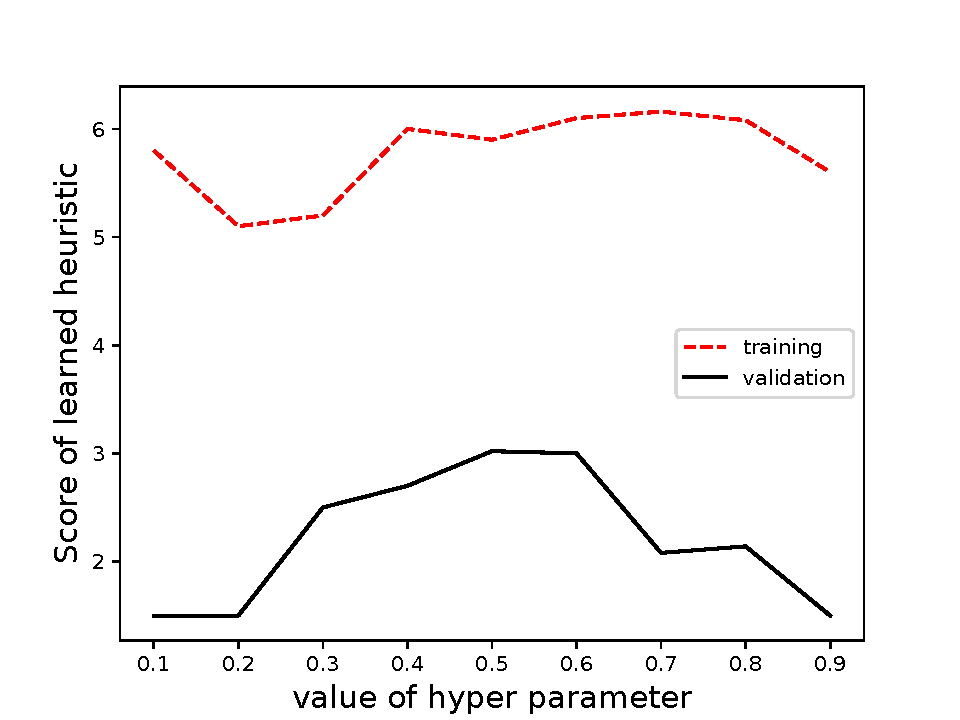
\includegraphics[width=6.3cm]{Graphick/figures/ctx_gamma.pdf}
	\caption{Object-sensitivity heuristic}
	\end{subfigure}
~\columnbreak

	\begin{subfigure}[t]{1.\columnwidth}
	\centering	
	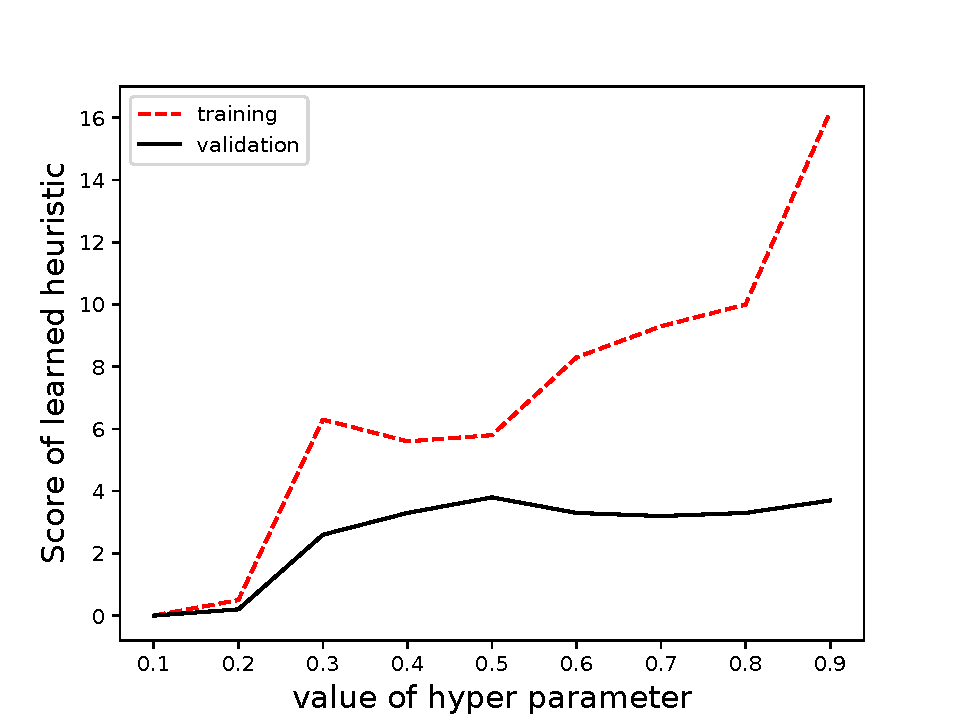
\includegraphics[width=6.3cm]{Graphick/figures/heap_gamma.pdf}
	\caption{Heap abstraction heuristic}
	\end{subfigure}
	\end{multicols}
	\caption{How score of learned heuristic changes over the value of $\hyper$.}
	\label{fig:gamma}
\end{figure}


\myparagraph{Choosing Hyper-Parameter $\hyper$}\label{sec:hyper_param}

Through our evaluation, we observed that the value of the hyper-parameter $\hyper$ plays an important role in the performance of the learned heuristic.
Figure~\ref{fig:gamma} depicts how performance of learned heuristics changes over the values of  $\hyper$.
The X-axis presents the value of $\hyper$ set to learn each heuristic, and
the Y-axis presents scores that we measured for performance of each heuristic $\heuristic_{\hyper}$ according to
${\sum_{P\in\vec{P}}\projproved(F_P(\heuristic_{\hyper}(G)))}\over{\sum_{P\in\vec{P}}
  \projcost(F_P(\heuristic_{\hyper}(G)))}$ where $\projcost$ denotes analysis time.
This score function presents the number of queries proved per second; thereby, more precise and scalable the analysis,
higher the score.
The red dotted and black solid lines present how the scores change over
the training programs $\vec{P}$ %(e.g., $\vec{P}$ = \{{\tt luindex,lusearch,antlr}\})
and the validation program, respectively.
For the training programs, the score of the learned heuristic increases as the higher $\hyper$ is given
because the heuristic becomes more fitted to the training programs.\footnote{It learned a bit bad heuristic when $\hyper$ is 0.9 in
  object-sensitivity heuristic because it is
difficult to generate specific features that satisfy such high precision
constraints; it eventually generates a general feature that include lots
of nodes.}
In our evaluation, both learned heuristics, however, perform the best on the validation program when $\hyper$ is 0.5;
thus, \OurCtx~in Table~\ref{tbl:contextAbstraction} and Table~\ref{tbl:heapAbstraction} corresponds to $\heuristic_{0.5}$.


%This occurs because the learned heuristics become overfitted to the training programs as the value of $\hyper$ increases;
%thus, simply increasing $\hyper$ is not an answer to achieve the best performance on validation and testing programs.







%\subsection{Learning Adequacy}

%\subsection{Insights from Generated Features}
\subsection{Learned Insights}

The learning algorithm generated 197 features in total for the object-sensitivity heuristic (68 features for 2-object-sensitivity, 29 for 2-type-sensitivity, and 100 features for 1-type-sensitivity). It generated 96 features for the heap abstraction heuristic.

\newcolumntype{P}[1]{>{\centering\arraybackslash}p{#1}}
\newcolumntype{M}[1]{>{\centering\arraybackslash}m{#1}}
\begin{figure}
\centering
\scriptsize
\setlength\extrarowheight{-1pt}
\begin{tabular}{|c|c|c| c | c | c |}
\toprule
\multicolumn{1}{|c}{}
                                                &                        & \multicolumn{1}{c|}{\textsf{Top 5 Features}} & \textsf{portion}
&\textsf{score} &
\multicolumn{1}{c|}{
\makecell{\textsf{Concretization}\\(Top 1)}
} \\ \midrule

\multirow{30}{*}{\rotatebox[origin=c]{90}{Object-Sensitivity Heuristic}}
& \multirow{10}{*}{\rotatebox[origin=c]{90}{1type}} &
\multirow{2}{*}{
\resizebox{0.40\columnwidth}{!}{
	\begin{tikzpicture}
	\node [block3,fill = gray] (n2) {{\tt\small [0,$\infty$],[61,$\infty$]}};
	\node [block3,right = 0.8cm of n2] (n3) {{\tt\small [46,$\infty$],[0,$\infty$]}};
	\path [line] (n2) -> (n3);
	\end{tikzpicture}
}
}
&\multirow{2}{*}{47\%} &\multirow{2}{*}{0.57}
                                        & \multirow{10}{*}{
		\resizebox{0.15\columnwidth}{!}{
			\begin{tikzpicture}
			\node [shape=circle,fill = gray,draw=black] (n1) {{\tt
                            n2}};
			\node [shape=circle,fill = gray,draw=black,left = 0.3cm
                        of n1] (n1left) {{\tt n1}};
			\node [shape=circle,fill = gray,draw=black,right = 0.3cm
                        of n1] (n1right) {{\tt n3}};
			\node [None,above = 0.7cm
                        of n1] (aboven1) {};
			\node [None,above = 0.7cm
                        of n1left] (aboven2) {};
			\node [None,above = 0.7cm
                        of n1right] (aboven3) {};
			\node [shape=circle,draw=black,below = 0.9cm
                        of n1] (n2) {{\tt n4}};
			\node [None,above left = 0.6 and 0.1cm
                        of n1] (n4) {};
			\node [None,right = 0.7cm
                        of n4] (n5) {};
			\node [None,above left = 0.7 and 0.5cm
                        of n2] (d1) {};
			\node [None, right = -0.1
                        of d1] (d2) {};
			\node [None, right = -0.1
                        of d2] (d3) {};
			\node [None, right = -0.1
                        of d3] (d4) {};
			\node [None, right = -0.1
                        of d4] (d5) {};
			\node [None, right = -0.1
                        of d5] (d6) {};
			\node [None, right = -0.1
                        of d6] (d7) {};
			\node [None, right = -0.1
                        of d7] (d8) {};
			\node [None, right = -0.1
                        of d8] (d9) {};
			\node [None, right = -0.1
                        of d9] (d10) {};
			\node [None, right = -0.1
                        of d10] (d11) {};
			\node [None, right = -0.1
                        of d11] (d12) {};
			\node [None, right = -0.1
                        of d12] (d13) {};		
			\path [line] (aboven1) -- (n1);
			\path [line] (aboven2) -- (n1left);
			\path [line] (aboven3) -- (n1right);
			\path [line] (n1left) -- (n2);
			\path [line] (n1right) -- (n2);
			\path [line] (n1) -- (n2);
			\path [line] (d1) -- (n2);
			\path [line] (d2) -- (n2);
			\path [line] (d3) -- (n2);
			\path [line] (d4) -- (n2);
			\path [line] (d5) -- (n2);
			\path [line] (d6) -- (n2);
			\path [line] (d7) -- (n2);
			\path [line] (d8) -- (n2);
			\path [line] (d9) -- (n2);
			\path [line] (d10) -- (n2);
			\path [line] (d11) -- (n2);
			\path [line] (d12) -- (n2);
			\path [line] (d13) -- (n2);
			\end{tikzpicture}
		}
}
                   \\
&&\multicolumn{1}{c|}{}&\multicolumn{1}{c|}{}  &\multicolumn{1}{c|}{}&\multicolumn{1}{c|}{}

\\
                                                &                        &
\multirow{2}{*}{
\resizebox{0.40\columnwidth}{!}{
	\begin{tikzpicture}
	\node [block3,fill = gray] (n2) {{\tt\small [0,$\infty$],[0,$\infty$]}};
	\node [block4,right = 0.8cm of n2] (n3) {{\tt\small [0,$\infty$],[117,$\infty$]}};
	\path [line] (n2) -> (n3);
	\end{tikzpicture}
}}
& \multirow{2}{*}{36\%} &\multirow{2}{*}{0.63}                                        &                                     \\
&&\multicolumn{1}{c|}{}&\multicolumn{1}{c|}{}  &\multicolumn{1}{c|}{}&\multicolumn{1}{c|}{}
\\
                                                &                        &
\multirow{2}{*}{
\resizebox{0.41\columnwidth}{!}{
	\begin{tikzpicture}
	\node [block4] (n2) {{\tt\small [0,$\infty$],[100,$\infty$]}};
	\node [block3,fill = gray,right = 0.8cm of n2] (n3) {{\tt\small [0,$\infty$],[29,$\infty$]}};
	\path [line] (n2) -> (n3);
	\end{tikzpicture}
}}
& \multirow{2}{*}{35\%} & \multirow{2}{*}{0.55}                                      &                                     \\
&&\multicolumn{1}{c|}{}&\multicolumn{1}{c|}{}  &\multicolumn{1}{c|}{}&\multicolumn{1}{c|}{}
\\
                                                &                        &
\multirow{2}{*}{
\resizebox{0.50\columnwidth}{!}{
	\begin{tikzpicture}
	\node [block4] (n2) {{\tt\small [0,$\infty$],[100,$\infty$]}};
	\node [block3,fill = gray,right = 0.3cm of n2] (n3) {{\tt\small [0,$\infty$],[0,$\infty$]}};
	\node [block4,right = 0.3cm of n3] (n4) {{\tt\small [0,$\infty$],[36,43]}};
	\path [line] (n2) -> (n3);
	\path [line] (n3) -> (n4);
	\end{tikzpicture}
}}
& \multirow{2}{*}{29\%} & \multirow{2}{*}{0.71}                                          &                                     \\
&&\multicolumn{1}{c|}{}&\multicolumn{1}{c|}{}  &\multicolumn{1}{c|}{}&\multicolumn{1}{c|}{}
\\


                                                &                        &
\multirow{2}{*}{
\resizebox{0.5\columnwidth}{!}{
	\begin{tikzpicture}
	\node [block4] (n2) {{\tt\small [0,$\infty$],[109,$\infty$]}};
	\node [block3,fill = gray,right = 0.3cm of n2] (n3) {{\tt\small [0,$\infty$],[0,$\infty$]}};
	\node [block4,right = 0.3cm of n3] (n4) {{\tt\small [171,$\infty$],[0,$\infty$]}};
	\path [line] (n2) -> (n3);
	\path [line] (n3) -> (n4);
	\end{tikzpicture}
}}
&\multirow{2}{*}{25\%}&\multirow{2}{*}{0.57}                                       &                                     \\
&&\multicolumn{1}{c|}{}&\multicolumn{1}{c|}{}  &\multicolumn{1}{c|}{}&\multicolumn{1}{c|}{}\\





\cline{2-6}
                                                & \multirow{10}{*}{\rotatebox[origin=c]{90}{2type}} &
\multirow{2}{*}{
\resizebox{0.40\columnwidth}{!}{
	\begin{tikzpicture}
	\node [block3] (n2) {{\tt\small [0,$\infty$],[36,39]}};
	\node [None ,above = 0.0cm of n2] (None) {};
	\node [block4 ,fill = gray,right = 0.8cm of n2] (n3) {{\tt\small [0,$\infty$],[73,75]}};
	\path [line] (n2) -> (n3);
	\end{tikzpicture}
}}
& \multirow{2}{*}{9\%}&\multirow{2}{*}{0.66}
                                                                                         & \multirow{10}{*}{
		\resizebox{0.15\columnwidth}{!}{
			\begin{tikzpicture}
			\node [shape=circle,fill = gray,draw=black] (n1) {{\tt
                            n2}};
			\node [shape=circle,draw=black,above = 0.5cm
                        of n1] (n0) {{\tt n1}};
			\node [None,below = 0.3cm
                        of n2] (bot) {};
			\node [None,right = 0.3cm
                        of n1] (n3) {};
			\node [None,above left = 0.4 and 0.5cm
                        of n0] (1d1) {};
			\node [None, right = -0.1
                        of 1d1] (1d2) {};
			\node [None, right = -0.1
                        of 1d2] (1d3) {};
			\node [None, right = -0.1
                        of 1d3] (1d4) {};
			\node [None, right = -0.1
                        of 1d4] (1d5) {};
			\node [None, right = -0.1
                        of 1d5] (1d6) {};
			\node [None, right = -0.1
                        of 1d6] (1d7) {};
			\node [None, right = -0.1
                        of 1d7] (1d8) {};
			\node [None, right = -0.1
                        of 1d8] (1d9) {};
			\node [None, right = -0.1
                        of 1d9] (1d10) {};
			\node [None, right = -0.1
                        of 1d10] (1d11) {};
			\node [None, right = -0.1
                        of 1d11] (1d12) {};
			\node [None, right = -0.1
                        of 1d12] (1d13) {};
			\node [None,below left = 0.3 and 0.7cm
                        of n0] (1e1) {};
			\node [None, right = -0.1
                        of 1e1] (1e2) {};
			\node [None, right = -0.1
                        of 1e2] (1e3) {};
			\node [None, right = -0.1
                        of 1e3] (1e4) {};
			\node [None, right = -0.1
                        of 1e4] (1e5) {};
			\node [None, right = -0.1
                        of 1e5] (1e6) {};
			\node [None, right = -0.1
                        of 1e6] (1e7) {};
			\node [None, right = -0.1
                        of 1e7] (1e8) {};
			\node [None, right = -0.1
                        of 1e8] (1e9) {};
			\node [None, right = -0.1
                        of 1e9] (1e10) {};
			\node [None, right = -0.1
                        of 1e10] (1e11) {};
			\node [None, right = -0.1
                        of 1e11] (1e12) {};
			\node [None, right = -0.1
                        of 1e12] (1e13) {};
			\node [None, right = -0.1
                        of 1e13] (1e14) {};
			\node [None, right = -0.1
                        of 1e14] (1e15) {};		
			\node [None,above left = 0.4 and 0.5cm
                        of n1] (d1) {};
			\node [None, right = -0.1
                        of d1] (d2) {};
			\node [None, right = -0.1
                        of d2] (d3) {};
			\node [None, right = -0.1
                        of d3] (d4) {};
			\node [None, right = -0.1
                        of d4] (d5) {};
			\node [None, right = -0.1
                        of d5] (d6) {};
			\node [None, right = -0.1
                        of d6] (d7) {};
			\node [None, right = -0.1
                        of d7] (d8) {};
			\node [None, right = -0.1
                        of d8] (d9) {};
			\node [None, right = -0.1
                        of d9] (d10) {};
			\node [None, right = -0.1
                        of d10] (d11) {};
			\node [None, right = -0.1
                        of d11] (d12) {};
			\node [None, right = -0.1
                        of d12] (d13) {};
			\node [None,below left = 0.5 and 0.7cm
                        of n1] (e1) {};
			\node [None, right = -0.1
                        of e1] (e2) {};
			\node [None, right = -0.1
                        of e2] (e3) {};
			\node [None, right = -0.1
                        of e3] (e4) {};
			\node [None, right = -0.1
                        of e4] (e5) {};
			\node [None, right = -0.1
                        of e5] (e6) {};
			\node [None, right = -0.1
                        of e6] (e7) {};
			\node [None, right = -0.1
                        of e7] (e8) {};
			\node [None, right = -0.1
                        of e8] (e9) {};
			\node [None, right = -0.1
                        of e9] (e10) {};
			\node [None, right = -0.1
                        of e10] (e11) {};
			\node [None, right = -0.1
                        of e11] (e12) {};
			\node [None, right = -0.1
                        of e12] (e13) {};
			\node [None, right = -0.1
                        of e13] (e14) {};
			\node [None, right = -0.1
                        of e14] (e15) {};			
%			\path [line] (n0) -- (1e1);
			\path [line] (n0) -- (1e2);
			\path [line] (n0) -- (1e3);
			\path [line] (n0) -- (1e4);
			\path [line] (n0) -- (1e5);
			\path [line] (n0) -- (1e6);
			\path [line] (n0) -- (1e7);
			\path [line] (n0) -- (1e8);
			\path [line] (n0) -- (1e9);
			\path [line] (n0) -- (1e10);
			\path [line] (n0) -- (1e11);
			\path [line] (n0) -- (1e12);
			\path [line] (n0) -- (1e13);
			\path [line] (n0) -- (1e14);
%			\path [line] (n0) -- (1e15);
			\path [line] (n0) -- (n1);
%			\path [line] (n1) -- (e1);
			\path [line] (n1) -- (e2);
			\path [line] (n1) -- (e3);
			\path [line] (n1) -- (e4);
			\path [line] (n1) -- (e5);
			\path [line] (n1) -- (e6);
			\path [line] (n1) -- (e7);
			\path [line] (n1) -- (e8);
			\path [line] (n1) -- (e9);
			\path [line] (n1) -- (e10);
			\path [line] (n1) -- (e11);
			\path [line] (n1) -- (e12);
			\path [line] (n1) -- (e13);
			\path [line] (n1) -- (e14);
%			\path [line] (n1) -- (e15);
			\end{tikzpicture}
		}
}                   \\
&&\multicolumn{1}{c|}{}&\multicolumn{1}{c|}{}  &\multicolumn{1}{c|}{}&\multicolumn{1}{c|}{}
\\
                                                &                        &
\multirow{2}{*}{
\resizebox{0.18\columnwidth}{!}{
	\begin{tikzpicture}
	\node [block4,fill = gray] (n2) {{\tt\small [105,155],[0,$\infty$]}};
	\end{tikzpicture}
}}
&\multirow{2}{*}{9\%}&\multirow{2}{*}{1} 
&                                     \\
&&\multicolumn{1}{c|}{}&\multicolumn{1}{c|}{}  &\multicolumn{1}{c|}{}&\multicolumn{1}{c|}{}
\\
                                                &                        &
\multirow{2}{*}{
\resizebox{0.5\columnwidth}{!}{
	\begin{tikzpicture}
	\node [block3] (n2) {{\tt\small [0,$\infty$],[0,61]}};
	\node [block4,fill = gray,right = 0.3cm of n2] (n3) {{\tt\small [60,76],[0,61]}};
	\node [block3,right = 0.3cm of n3] (n4) {{\tt\small [0,22],[0,$\infty$]}};
	\path [line] (n2) -> (n3);
	\path [line] (n3) -> (n4);
	\end{tikzpicture}
}}
& \multirow{2}{*}{9\%} &\multirow{2}{*}{0.5}                                          &                                     \\
&&\multicolumn{1}{c|}{}&\multicolumn{1}{c|}{}  &\multicolumn{1}{c|}{}&\multicolumn{1}{c|}{}
\\
                                                &                        &
\multirow{2}{*}{
\resizebox{0.5\columnwidth}{!}{
	\begin{tikzpicture}
	\node [block3] (n2) {{\tt\small [0,$\infty$],[29,61]}};
	\node [block4,fill = gray,right = 0.3cm of n2] (n3) {{\tt\small [171,228],[0,$\infty$]}};
	\node [block3,right = 0.3cm of n3] (n4) {{\tt\small [0,46],[0,$\infty$]}};
	\path [line] (n2) -> (n3);
	\path [line] (n3) -> (n4);
	\end{tikzpicture}
}}
&\multirow{2}{*}{4\%} &\multirow{2}{*}{1}                                       &                                     \\
&&\multicolumn{1}{c|}{}&\multicolumn{1}{c|}{}  &\multicolumn{1}{c|}{}&\multicolumn{1}{c|}{}
\\
                                                &                        &
\multirow{2}{*}{
\resizebox{0.18\columnwidth}{!}{
	\begin{tikzpicture}
	\node [block3,fill = gray] (n2) {{\tt\small [84,91],[0,$\infty$]}};
	\end{tikzpicture}
}}
& \multirow{2}{*}{4\%} & \multirow{2}{*}{0.5}                                      &                                     \\
&&\multicolumn{1}{c|}{}&\multicolumn{1}{c|}{}  &\multicolumn{1}{c|}{}&\multicolumn{1}{c|}{}
\\
\cline{2-6}
 & \multirow{10}{*}{\rotatebox[origin=c]{90}{2obj}}  &
\multirow{2}{*}{
\resizebox{0.17\columnwidth}{!}{
	\begin{tikzpicture}
	\node [block3,fill = gray] (n2) {{\tt\small [0,$\infty$],[53,61]}};
	\node [None ,above = 0.0cm of n2] (None) {};
	\end{tikzpicture}
}}
& \multirow{2}{*}{9\%} & \multirow{2}{*}{0.53}
& \multirow{10}{*}{
\resizebox{0.15\columnwidth}{!}{
			\begin{tikzpicture}
			\node [None] (n1) {};
			\node [shape=circle,fill=gray,draw=black,below = 0.9cm
                        of n1] (n2) {{\tt n1}};
			\node [None,right = 0.3cm
                        of n1] (n3) {};
			\node [None,above left = 0.7 and 0.5cm
                        of n2] (d1) {};
			\node [None, right = -0.1
                        of d1] (d2) {};
			\node [None, right = -0.1
                        of d2] (d3) {};
			\node [None, right = -0.1
                        of d3] (d4) {};
			\node [None, right = -0.1
                        of d4] (d5) {};
			\node [None, right = -0.1
                        of d5] (d6) {};
			\node [None, right = -0.1
                        of d6] (d7) {};
			\node [None, right = -0.1
                        of d7] (d8) {};
			\node [None, right = -0.1
                        of d8] (d9) {};
			\node [None, right = -0.1
                        of d9] (d10) {};
			\node [None, right = -0.1
                        of d10] (d11) {};
			\node [None, right = -0.1
                        of d11] (d12) {};
			\node [None, right = -0.1
                        of d12] (d13) {};
			\node [None,below left = 0.9 and 0.7cm
                        of n2] (e1) {};
			\node [None, right = -0.1
                        of e1] (e2) {};
			\node [None, right = -0.1
                        of e2] (e3) {};
			\node [None, right = -0.1
                        of e3] (e4) {};
			\node [None, right = -0.1
                        of e4] (e5) {};
			\node [None, right = -0.1
                        of e5] (e6) {};
			\node [None, right = -0.1
                        of e6] (e7) {};
			\node [None, right = -0.1
                        of e7] (e8) {};
			\node [None, right = -0.1
                        of e8] (e9) {};
			\node [None, right = -0.1
                        of e9] (e10) {};
			\node [None, right = -0.1
                        of e10] (e11) {};
			\node [None, right = -0.1
                        of e11] (e12) {};
			\node [None, right = -0.1
                        of e12] (e13) {};
			\node [None, right = -0.1
                        of e13] (e14) {};
			\node [None, right = -0.1
                        of e14] (e15) {};			
			\path [line] (n1) -- (n2);
%			\path [line] (n2) -- (e1);
			\path [line] (n2) -- (e2);
			\path [line] (n2) -- (e3);
			\path [line] (n2) -- (e4);
			\path [line] (n2) -- (e5);
			\path [line] (n2) -- (e6);
			\path [line] (n2) -- (e7);
			\path [line] (n2) -- (e8);
			\path [line] (n2) -- (e9);
			\path [line] (n2) -- (e10);
			\path [line] (n2) -- (e11);
			\path [line] (n2) -- (e12);
			\path [line] (n2) -- (e13);
			\path [line] (n2) -- (e14);
%			\path [line] (n2) -- (e15);
			\end{tikzpicture}
		}
}                   \\
&&\multicolumn{1}{c|}{}&\multicolumn{1}{c|}{}  &\multicolumn{1}{c|}{}&\multicolumn{1}{c|}{}
\\
                                                &
                                                                        &
\multirow{2}{*}{
\resizebox{0.17\columnwidth}{!}{
\begin{tikzpicture}
\node [block3,fill = gray] (n2) {{\tt\small [0,$\infty$],[24,25]}};
\end{tikzpicture}
}}
&\multirow{2}{*}{6\%} &\multirow{2}{*}{0.53}                                       &                                     \\
&&\multicolumn{1}{c|}{}&\multicolumn{1}{c|}{}  &\multicolumn{1}{c|}{}&\multicolumn{1}{c|}{}
\\
                                                &                        &
\multirow{2}{*}{\resizebox{0.5\columnwidth}{!}{
	\begin{tikzpicture}
	\node [block4,fill = gray] (n2) {{\tt\small [0,$\infty$],[0,7]}};
	\node [block3,right = 0.3cm of n2] (n3) {{\tt\small [9,11],[0,$\infty$]}};
	\node [block3,right = 0.3cm of n3] (n4) {{\tt\small [76,$\infty$],[0,$\infty$]}};
	\path [line] (n2) -> (n3);
	\path [line] (n3) -> (n4);
	\end{tikzpicture}
}}
&\multirow{2}{*}{2\%}&\multirow{2}{*}{0.82}                                        & \\
&&\multicolumn{1}{c|}{}&\multicolumn{1}{c|}{}  &\multicolumn{1}{c|}{}&\multicolumn{1}{c|}{}
\\

                                                &                        &
\multirow{2}{*}{\resizebox{0.5\columnwidth}{!}{
	\begin{tikzpicture}
	\node [block4] (n2) {{\tt\small [0,$\infty$],[43,$\infty$]}};
	\node [block3,fill = gray,right = 0.3cm of n2] (n3) {{\tt\small [0,$\infty$],[0,14]}};
	\node [block3,right = 0.3cm of n3] (n4) {{\tt\small [22,24],[0,$\infty$]}};
	\path [line] (n2) -> (n3);
	\path [line] (n3) -> (n4);
	\end{tikzpicture}
}}
&\multirow{2}{*}{1\%}&\multirow{2}{*}{0.63}                                        &                                     \\
&&\multicolumn{1}{c|}{}&\multicolumn{1}{c|}{}  &\multicolumn{1}{c|}{}&\multicolumn{1}{c|}{}
\\
                                                &
                                                                        &
\multirow{2}{*}{\resizebox{0.5\columnwidth}{!}{
	\begin{tikzpicture}
	\node [block4] (n2) {{\tt\small [0,$\infty$],[145,147]}};
	\node [block3,fill = gray,right = 0.3cm of n2] (n3) {{\tt\small [0,$\infty$],[0,$\infty$]}};
	\node [block3,right = 0.3cm of n3] (n4) {{\tt\small [0,46],[0,$\infty$]}};
	\path [line] (n2) -> (n3);
	\path [line] (n3) -> (n4);
	\end{tikzpicture}
}}                                                                                &\multirow{2}{*}{1\%}&\multirow{2}{*}{0.69}&                                     \\
&&\multicolumn{1}{c|}{}&\multicolumn{1}{c|}{}  &\multicolumn{1}{c|}{}&\multicolumn{1}{c|}{}
\\

%                                                &                        &
%\resizebox{0.45\columnwidth}{!}{
%	\begin{tikzpicture}
%	\node [block3,fill = gray] (n2) {{\tt\small [0,$\infty$],[0,3]}};
%	\node [block4,right = 0.8cm of n2] (n3) {{\tt\small [22,33],[0,$\infty$]}};
%	\path [line] (n2) -> (n3);
%	\end{tikzpicture}
%}                                       &                                     \\
 \midrule\midrule
\multicolumn{2}{|c|}{\multirow{10}{*}{
		\rotatebox[origin=c]{90}{\makecell{Heap Abstraction\\Heuristic}}}}        &
\multirow{2}{*}{\resizebox{0.5\columnwidth}{!}{
	\begin{tikzpicture}
	\node [block3,fill = gray] (n2) {{\tt\small [0,$\infty$],[0,3]}};
	\node [block4,right = 0.3cm of n2] (n3) {{\tt\small [48,$\infty$],[0,$\infty$]}};
	\node [block4,right = 0.3cm of n3] (n4) {{\tt\small [0,$\infty$],[140,$\infty$]}};
	\path [line] (n2) -> (n3);
	\path [line] (n3) -> (n4);
	\end{tikzpicture}
}}
& \multirow{2}{*}{35\%} &\multirow{2}{*}{0.61} 

& \multirow{10}{*}{
		\resizebox{0.15\columnwidth}{!}{
			\begin{tikzpicture}
			\node [shape=circle,fill = gray,draw=black] (n1) {{\tt
                            n1}};
			\node [shape=circle,draw=black,below = 0.6cm
                        of n1] (n2) {{\tt n2}};
			\node [shape=circle,draw=black,below = 0.6cm
                        of n2] (n4) {{\tt n3}};
			\node [None,right = 0.3cm
                        of n1] (n3) {};
			\node [None,above left = 0.5 and 0.5cm
                        of n2] (d1) {};
			\node [None, right = -0.1
                        of d1] (d2) {};
			\node [None, right = -0.1
                        of d2] (d3) {};
			\node [None, right = -0.1
                        of d3] (d4) {};
			\node [None, right = -0.1
                        of d4] (d5) {};
			\node [None, right = -0.1
                        of d5] (d6) {};
			\node [None, right = -0.1
                        of d6] (d7) {};
			\node [None, right = -0.1
                        of d7] (d8) {};
			\node [None, right = -0.1
                        of d8] (d9) {};
			\node [None, right = -0.1
                        of d9] (d10) {};
			\node [None, right = -0.1
                        of d10] (d11) {};
			\node [None, right = -0.1
                        of d11] (d12) {};
			\node [None, right = -0.1
                        of d12] (d13) {};
			\node [None,below left = 0.4 and 0.7cm
                        of n2] (e1) {};
			\node [None, right = -0.1
                        of e1] (e2) {};
			\node [None, right = -0.1
                        of e2] (e3) {};
			\node [None, right = -0.1
                        of e3] (e4) {};
			\node [None, right = -0.1
                        of e4] (e5) {};
			\node [None, right = -0.1
                        of e5] (e6) {};
			\node [None, right = -0.1
                        of e6] (e7) {};
			\node [None, right = -0.1
                        of e7] (e8) {};
			\node [None, right = -0.1
                        of e8] (e9) {};
			\node [None, right = -0.1
                        of e9] (e10) {};
			\node [None, right = -0.1
                        of e10] (e11) {};
			\node [None, right = -0.1
                        of e11] (e12) {};
			\node [None, right = -0.1
                        of e12] (e13) {};
			\node [None, right = -0.1
                        of e13] (e14) {};
			\node [None, right = -0.1
                        of e14] (e15) {};	
			\node [None,above left = 0.3 and 0.5cm
                        of n4] (1d1) {};
			\node [None, right = -0.1
                        of 1d1] (1d2) {};
			\node [None, right = -0.1
                        of 1d2] (1d3) {};
			\node [None, right = -0.1
                        of 1d3] (1d4) {};
			\node [None, right = -0.1
                        of 1d4] (1d5) {};
			\node [None, right = -0.1
                        of 1d5] (1d6) {};
			\node [None, right = -0.1
                        of 1d6] (1d7) {};
			\node [None, right = -0.1
                        of 1d7] (1d8) {};
			\node [None, right = -0.1
                        of 1d8] (1d9) {};
			\node [None, right = -0.1
                        of 1d9] (1d10) {};
			\node [None, right = -0.1
                        of 1d10] (1d11) {};
			\node [None, right = -0.1
                        of 1d11] (1d12) {};
			\node [None, right = -0.1
                        of 1d12] (1d13) {};
			\node [None,below left = 0.5 and 0.7cm
                        of n4] (1e1) {};
			\node [None, right = -0.1
                        of 1e1] (1e2) {};
			\node [None, right = -0.1
                        of 1e2] (1e3) {};
			\node [None, right = -0.1
                        of 1e3] (1e4) {};
			\node [None, right = -0.1
                        of 1e4] (1e5) {};
			\node [None, right = -0.1
                        of 1e5] (1e6) {};
			\node [None, right = -0.1
                        of 1e6] (1e7) {};
			\node [None, right = -0.1
                        of 1e7] (1e8) {};
			\node [None, right = -0.1
                        of 1e8] (1e9) {};
			\node [None, right = -0.1
                        of 1e9] (1e10) {};
			\node [None, right = -0.1
                        of 1e10] (1e11) {};
			\node [None, right = -0.1
                        of 1e11] (1e12) {};
			\node [None, right = -0.1
                        of 1e12] (1e13) {};
			\node [None, right = -0.1
                        of 1e13] (1e14) {};
			\node [None, right = -0.1
                        of 1e14] (1e15) {};				
			\path [line] (n1) -- (n2);
			\path [line] (n1) -- (n3);
			\path [line] (d1) -- (n2);
			\path [line] (d2) -- (n2);
			\path [line] (d3) -- (n2);
			\path [line] (d4) -- (n2);
			\path [line] (d5) -- (n2);
			\path [line] (d6) -- (n2);
			\path [line] (d7) -- (n2);
			\path [line] (d8) -- (n2);
			\path [line] (d9) -- (n2);
			\path [line] (d10) -- (n2);
			\path [line] (d11) -- (n2);
			\path [line] (d12) -- (n2);
			\path [line] (d13) -- (n2);
%			\path [line] (n2) -- (e1);
			\path [line] (n2) -- (e2);
			\path [line] (n2) -- (e3);
			\path [line] (n2) -- (e4);
			\path [line] (n2) -- (e5);
			\path [line] (n2) -- (e6);
			\path [line] (n2) -- (e7);
			\path [line] (n2) -- (e8);
			\path [line] (n2) -- (e9);
			\path [line] (n2) -- (e10);
			\path [line] (n2) -- (e11);
			\path [line] (n2) -- (e12);
			\path [line] (n2) -- (e13);
			\path [line] (n2) -- (e14);
%			\path [line] (n2) -- (e15);
			\path [line] (n2) -- (n4);
			\path [line] (1d1) -- (n4);
			\path [line] (1d2) -- (n4);
			\path [line] (1d3) -- (n4);
			\path [line] (1d4) -- (n4);
			\path [line] (1d5) -- (n4);
			\path [line] (1d6) -- (n4);
			\path [line] (1d7) -- (n4);
			\path [line] (1d8) -- (n4);
			\path [line] (1d9) -- (n4);
			\path [line] (1d10) -- (n4);
			\path [line] (1d11) -- (n4);
			\path [line] (1d12) -- (n4);
			\path [line] (1d13) -- (n4);
%			\path [line] (n4) -- (1e1);
			\path [line] (n4) -- (1e2);
			\path [line] (n4) -- (1e3);
			\path [line] (n4) -- (1e4);
			\path [line] (n4) -- (1e5);
			\path [line] (n4) -- (1e6);
			\path [line] (n4) -- (1e7);
			\path [line] (n4) -- (1e8);
			\path [line] (n4) -- (1e9);
			\path [line] (n4) -- (1e10);
			\path [line] (n4) -- (1e11);
			\path [line] (n4) -- (1e12);
			\path [line] (n4) -- (1e13);
			\path [line] (n4) -- (1e14);
%			\path [line] (n4) -- (1e15);
			\end{tikzpicture}
		}
}\\
\multicolumn{1}{|c}{}&\multicolumn{1}{c|}{}&\multicolumn{1}{c|}{}&\multicolumn{1}{c|}{}  &\multicolumn{1}{c|}{}&\multicolumn{1}{c|}{}
\\
\multicolumn{2}{|l|}{}                                                   &
\multirow{2}{*}{\resizebox{0.5\columnwidth}{!}{
	\begin{tikzpicture}
	\node [block3,fill = gray] (n2) {{\tt\small [0,12],[0,3]}};
	\node [block4,right = 0.3cm of n2] (n3) {{\tt\small [0,97],[0,$\infty$]}};
	\node [block4,right = 0.3cm of n3] (n4) {{\tt\small [0,$\infty$],[140,$\infty$]}};
	\path [line] (n2) -> (n3);
	\path [line] (n3) -> (n4);
	\end{tikzpicture}
}}
&\multirow{2}{*}{33\%}
&\multirow{2}{*}{0.53}                                      &                                     \\
\multicolumn{1}{|c}{}&\multicolumn{1}{c|}{}&\multicolumn{1}{c|}{}&\multicolumn{1}{c|}{}  &\multicolumn{1}{c|}{}&\multicolumn{1}{c|}{}
\\
\multicolumn{2}{|l|}{}                                                   &
\multirow{2}{*}{\resizebox{0.40\columnwidth}{!}{
	\begin{tikzpicture}
	\node [block4,fill = gray] (n3) {{\tt\small [38,$\infty$],[0,62]}};
	\node [block4,right = 0.8cm of n3] (n4) {{\tt\small [0,$\infty$],[236,$\infty$]}};
	\path [line] (n3) -> (n4);
	\end{tikzpicture}
}}
& \multirow{2}{*}{27\%} &\multirow{2}{*}{0.59}                                        &                                     \\
\multicolumn{1}{|c}{}&\multicolumn{1}{c|}{}&\multicolumn{1}{c|}{}&\multicolumn{1}{c|}{}  &\multicolumn{1}{c|}{}&\multicolumn{1}{c|}{}
\\
\multicolumn{2}{|l|}{}                                                   &
\multirow{2}{*}{\resizebox{0.40\columnwidth}{!}{
	\begin{tikzpicture}
	\node [block4,fill = gray] (n3) {{\tt\small [0,48],[0,62]}};
	\node [block4,right = 0.8cm of n3] (n4) {{\tt\small [72,84],[0,$\infty$]}};
	\path [line] (n3) -> (n4);
	\end{tikzpicture}
}}
& \multirow{2}{*}{24\%} & \multirow{2}{*}{0.53} 
                                         &\\
\multicolumn{1}{|c}{}&\multicolumn{1}{c|}{}&\multicolumn{1}{c|}{}&\multicolumn{1}{c|}{}  &\multicolumn{1}{c|}{}&\multicolumn{1}{c|}{}
\\
\multicolumn{2}{|l|}{}                                                   &
\multirow{2}{*}{\resizebox{0.5\columnwidth}{!}{
	\begin{tikzpicture}
	\node [block3,fill = gray] (n2) {{\tt\small [0,24],[0,$\infty$]}};
	\node [block4,right = 0.3cm of n2] (n3) {{\tt\small [21,$\infty$],[140,$\infty$]}};
	\node [block4,right = 0.3cm of n3] (n4) {{\tt\small [0,97],[0,$\infty$]}};
	\path [line] (n2) -> (n3);
	\path [line] (n3) -> (n4);
	\end{tikzpicture}
}}
& \multirow{2}{*}{22\%} & \multirow{2}{*}{0.53} 
                                         &                                     \\
\multicolumn{1}{|c}{}&\multicolumn{1}{c|}{}&\multicolumn{1}{c|}{}&\multicolumn{1}{c|}{}  &\multicolumn{1}{c|}{}&\multicolumn{1}{c|}{}
\\
%\multicolumn{2}{|l|}{}                                                   &
%\resizebox{0.45\columnwidth}{!}{
%	\begin{tikzpicture}
%	\node [block3,fill = gray] (n2) {{\tt\small [0,48],[0,$\infty$]}};
%	\node [block4,right = 0.8cm of n2] (n3) {{\tt\small [72,84],[0,$\infty$]}};
%
%	\path [line] (n2) -> (n3);
%	\end{tikzpicture}
%}                                         &                                     \\
\bottomrule
\end{tabular}
\caption{Top-5 features learned by our technique, and concrete nodes implied by the top-1 feature.
%Gray colored abstract nodes in the features correspond to the target nodes and others are predecessors or successors.
%Gray colored nodes in the column \textsf{Concretization} are precision-critical nodes which are selected by the first features; 
%other nodes are predecessors or successors that make the gray colored nodes satisfy the features.
}
\label{fig:features}
\end{figure}



%%% Local Variables:
%%% mode: latex
%%% TeX-master: "paper"
%%% End:


\myparagraph{Top-5 Features}
Figure~\ref{fig:features} describes the most informative features generated by our technique for each abstraction degree and their concretization in the given graphs.
The second column \textsf{Top 5 Features}, in decreasing order of \textsf{portion}, presents top 5 features which have the greatest number of precision-critical nodes satisfying the features with scores above 0.5.
For example, the first feature in 1type contains 47\% nodes of the total precision-critical nodes which are to be applied 1-type-sensitivity,
and has a score of 0.57.
If a feature is too general (e.g., $(\epsilon, ([0,\infty],[0,\infty]), \epsilon)$), it is excluded even with a large portion (e.g., 100\%)
because its score is under 0.5.
Similarly, if a feature is too specific, it is also excluded because it includes a small number of precision-critical nodes even with a good score.
For the features, the gray colored abstract nodes correspond to the target one $\hat{n}$ in each feature
(e.g., $(\seq{\myhat{p}_0,\myhat{p}_1,\dots,\myhat{p}_q}, \myhat{n}, \seq{\myhat{s}_0,\myhat{s}_1,\dots,\myhat{s}_r}) \in \Feature$).
Other nodes are predecessors or successors of the target abstract nodes (e.g., $\myhat{p}_0$, $\myhat{s}_0$, and $\myhat{s}_1$).
For each feature, we show the number of satisfying nodes over the total precision-critical nodes in the given graphs (\textsf{portion}) and the scores (\textsf{score}).
The right most column, \textsf{Concretization}, illustrates the visualized concretization for each first feature in \textsf{Top 5 Features} column,
%in the real graphs over the training programs, where the gray colored nodes correspond to the target nodes of the first feature.
where the gray colored nodes correspond to the target abstract nodes of the first feature.
For space reasons, we draw each node to have at most 13 incoming and outgoing edges although it can have more than 13 edges.


\begin{table}[]
\setlength\extrarowheight{-1pt}
\caption{Performance of our manually-designed graph-based heap abstraction heuristic for FPG}
\label{tbl:principle}
\centering
\footnotesize
\begin{tabular}{@{}clrr | clrr@{}}
\toprule
benchmarks               & \multicolumn{1}{c}{} & \multicolumn{1}{c}{alarms} & \multicolumn{1}{c|}{time(s)} & benchmarks                & \multicolumn{1}{c}{} & \multicolumn{1}{c}{alarms} & \multicolumn{1}{c}{time(s)} \\ \midrule
\multirow{2}{*}{luindex} & \Principle              & 374                        & 29(+29)                         & \multirow{2}{*}{lusearch} & \Principle            & 388                        & 33(+31)                        \\
                         % & \OurHeap            & 358                        & 23                          &                           & \OurHeap              & 372                        & 21                          \\
                         & \AllocBased          & 358                        & 5,475                       &                           & \AllocBased          & -                          & $>$10,800        \\\midrule
\multirow{2}{*}{antlr}   & \Principle              & 478                        & 44(+47)                        & \multirow{2}{*}{pmd$_{m}$}      & \Principle            & 886                        & 83(+65)                          \\
                         % & \OurHeap            & 463                        & 49                          &                           & \OurHeap              & 871                        & 48                          \\
                         & \AllocBased          & 463                        & 5,241                       &                           & \AllocBased          & 871                        & 9,146                       \\\midrule
\multirow{2}{*}{fop}     & \Principle            & 391                        & 41(+46)                          & \multirow{2}{*}{xalan}    & \Principle            & 548                        & 841(+85)                         \\
                         % & \OurHeap              & 376                        & 30                          &                           & \OurHeap              & 539                        & 489                         \\
                         & \AllocBased          & -                          & $>$10,800        &                           & \AllocBased          & -                          & $>$10,800        \\ \bottomrule
\end{tabular}
\end{table}


\myparagraph{Insights}

The generated features during the learning process provide hints on designing analysis heuristics from the graphs.
For example, we investigated the features of the heap abstraction heuristic in Figure~\ref{fig:features} and found two commonalities in them.
First,  the features have the form of $(\epsilon,\hat{n}, \hat{\vec{s}})$ where $\hat{\vec{s}}$ is not $\epsilon$,
which implies that we should consider successors more than predecessors when designing heap abstraction heuristics from points-to graph.
The second commonality is that $\hat{\vec{s}}$ or $\hat{n}$ tends to include an abstract
node $\aNode$ that presents nodes with lots of outgoing edges, i.e., $\aNode =
(itv,[b,\infty])$ where the number $b$ is about $3\%$ of the total nodes in a graph of a training program.
From these observations, we manually designed a graph-based heap abstraction heuristic which
assigns allocation-site based heap abstraction to the target nodes
if at least $3\%$ of the total nodes in FPG belong to either the target node or its successor nodes
(i.e. $\heuristic = \seq{\{ (\epsilon,([0,\infty],[b',\infty]),\epsilon)
	,(\epsilon,\top,\seq{([0,\infty],[b',\infty])})
	,(\epsilon,\top,\seq{\top,([0,\infty],[b',\infty])})
	,\dots
	\}
}$ where $\top$ equals to the most general one $([0,\infty],[0,\infty])$ and $b'$ is 3\% of the total nodes in the given graph).
Otherwise, the heuristic assigns type-based heap abstraction to the others.
%where $\top$ equals to the most general abstract node $([0,\infty],[0,\infty])$, and $b$ equals to 3\% of the total nodes in the given graph).
Table~\ref{tbl:principle} demonstrates the performance of the manually-crafted heuristic.
In comparison to \AllocBased, it reduces about 99\% of analysis cost while producing only 2\% more alarms.
%Compared to the baseline heuristic~\AllocBased,



Intuitively, the nodes with lots of successors in FPG should be analyzed precisely because merging the objects with others would produce lots of spurious analysis results.
For example, if there exists an object with lots of field objects which we want to merge with another one with a few field objects,
it eventually produces lots of spurious results stating that the both heaps can have lots of field objects.
%Such insight is related with that of \Mahjong~which merges the two objects if they have the same types of successors because,
%statically, an object having lots of successors is hard to have exactly the same types of successors with other objects.
Such insight is related with that of \Mahjong~which merges the objects if their successors have the same type;
statistically, if an object has lots of successors, there hardly exist the other objects with exactly the same types of successors.
Surprisingly, it is easy to find such insight through the features generated by our technique.
Note that this insight is general as it is not dependent to Java programs.
For example, when analyzing a C program, it is a required task not to merge such heaps with others as it would produce lots of spurious results.

%\textcolor{black}{
%\myparagraph{Graphick vs Scaler}
%Interestingly, Figure~\ref{fig:features} shows that the insight learned statistically can differ from the logic-based insight
%through the difference between \OurCtx~and \Scaler~in deciding which nodes to analyze more precisely.
Interestingly, Figure~\ref{fig:features} also shows the difference between the statistically-learned insight behind \OurCtx~and the logical insight behind \Scaler~in deciding which nodes to analyze more precisely.
Based on the logical insight, \Scaler~relies heavily on the number of incoming edges
as that number in the object allocation graph indicates %{\color{red}{
how many contexts will be constructed in object sensitivity.%}}
~\ourtool, however, treats the number of neighbor nodes' outgoing edges more importantly, as shown in Figure 6.
Such differences result in the performance gap between the two object-sensitivity heuristics.
%which shows better performance in both precision and scalability than the logic-based insight.
%}

%\textcolor{red}{
\myparagraph{Generality of learned heuristic}
We found the learned heuristic for object sensitivity is general to the hybrid-context sensitivity~\cite{KastrinisS13a}. Table~\ref{tbl:hybrid} presents the performance of the conventional 2-hybrid-context sensitivity (\twosobjH) and
2-hybrid-context sensitivity with the learned heuristic (\ourtool) used in Section~\ref{sec:comparescaler}.
%when using 6 DaCapo benchmark programs as testing programs.
The table shows that \ourtool~is also cost-effective compared to \twosobjH. For example, on a test program bloat,
\ourtool~produces only 22 more alarms while reducing about 90\% of analysis costs.
%}



\begin{table}[]
\setlength\extrarowheight{-1pt}
\caption{Performance comparison between conventional 2-hybrid-context-sensitivity (\twosobjH) and 2-hybrid-context-sensitivity with our learned heuristic for 2-object-sensitivity (\ourtool).}
\label{tbl:hybrid}
\centering\footnotesize
\begin{tabular}{@{}clrrrrrr@{}}
\toprule
                          & \multicolumn{1}{c}{} & \multicolumn{1}{c}{pmd$_m$} & \multicolumn{1}{c}{chart} & \multicolumn{1}{c}{eclipse} & \multicolumn{1}{c}{xalan} & \multicolumn{1}{c}{fop} & \multicolumn{1}{c}{bloat}  \\ \midrule
\multirow{2}{*}{\ourtool} & \#may-fail casts     & 220                      & 867                       & 2,880                        & 479                       & 1,408                    & 1,147                      \\
                          & analysis time (s)    & 45+(78)                  & 83(+76)                   & 1,426(+105)                  & 185(+57)                  & 245(+85)                & 215(+30)                  \\ \midrule
\multirow{2}{*}{\twosobjH}    & \#may-fail casts     & 220                      & 757                       & -                       & 447                          &  1,295                       & 1,125                          \\
                          & analysis time (s)    & 42                       & 195                       & $>$ 10,800                            & 428                          & 818                        & 2,238                           \\
%\midrule
%\multirow{2}{*}{\Insens}   & \#may-fail casts     & 679                      & 1,810                      & 4190                        & 1,182                      & 2,458                    & 1,924                      \\
%                          & analysis time (s)    & 23                       & 48                        & 91                          & 37                        & 53                      & 20                        \\
\bottomrule
\end{tabular}
\end{table}




%%% Local Variables:
%%% mode: latex
%%% TeX-master: "paper"
%%% End:

% !TEX root = ./paper.tex

\subsection{Performance Variations on Different Training Datasets}\label{sec:justify}

We constructed a benchmark suite with the programs from the DaCapo suite,
and used 3$\sim$4 small programs (i.e. luindex, lusearch, antlr, and pmd$_{m}$) as our training set.
In this subsection, we evaluate \ourtool~on different combinations of training data to see how its performance is affected by the number of training programs.

%Despite the small number and small size, they provide sufficient information to learn cost-effective heuristics,
%and we conducted an additional experiment to justify this evaluation setting.


We found that the amount of training data is overall critical, and
using four small programs as a training set can produce competitive heap abstraction heuristics cost-effectively.
Table~\ref{tbl:training} presents the performance and scores
(i.e. ${\mbox{\#proven casts}}\over{\mbox{analysis time (s)}}$)
of each heuristic learned with various combinations of training programs (i.e., \onepgm, \twopgm, \threepgm, and \fourpgm) and an ideal heuristic (\ideal) against the validation program findbugs.
For the ideal heuristic (\ideal), we assume that it has the precision of \Mahjong~and the scalability of \TypeBased~
since they are the most precise and the most scalable respectively in our space of heap abstraction heuristic.
The second row, analysis time (s), in table~\ref{tbl:training} indicates the amount of time each heuristic took to successfully analyze the validation program, and
the third row, \#proven casts, presents the number of castings proved to be safe;
thereby, the more precise the analysis, the greater the number of proven casts.
As shown in Table~\ref{tbl:training}, the score increases with respect to the size of training set.
The score of \fourpgm~(i.e. 13.6) is nearly the same with that of the ideal heuristic (i.e. 15.4) in our evaluation.
It implies that using four programs as a training set is sufficient to produce cost-effective heap abstraction heuristics.


% among the various combinations of our training programs.
%In Table~\ref{tbl:training}, \onepgm, \twopgm, \threepgm, and \fourpgm correspond to the heuristics learned with
%{\it npgm} $(1 \le n\le 4)$ indicates the number of training programs used for learning heuristics.
%We calculate the cost of the ideal heuristic with the cost of \TypeBased~and the proven queries by \Mahjong~
%because \TypeBased~is most scalable
%and \Mahjong~is most precise in our space of heap abstraction heuristics.
%
%
%The row score present the quality of the learned heuristics and an ideal heuristic
%
%The black solid line and red dotted line in the graph present the scores of our learned heuristics and an ideal heuristic (i.e.,
%${\small {\mbox{proven queries in \Mahjong}}\over{
%\mbox{cost of \TypeBased}}}$),
%respectively.
%We calculate the cost of the ideal heuristic with the cost of \TypeBased~and the proven queries by \Mahjong~
%because \TypeBased~is most scalable
%and \Mahjong~is most precise in our space of heap abstraction heuristics.
%\minseok{revision}

%In our experiments, we used 3 $\sim$ 4 programs for our training set.

%\textcolor{red}{
%Although we used a small number of small programs (e.g., luindex, lusearch, antlr, pmd$_{m}$) as a training set, those training programs do not represent unrealistic training data.

Using four programs as training programs could produce cost-effective heuristics because, even though our training programs are the smallest among the total benchmark programs,
they still provide sufficient learning data for our approach.
First, the DaCapo suite itself is a collection of realistic programs.
DaCapo has been carefully designed to include various behaviors and complex codes~\cite{Blackburn2006}.
For example, even the smallest program (i.e. lusearch) in Dacapo has more methods than the largest one in the SPEC benchmark~\cite{specjvm98}.
Secondly, when training heuristics in our approach, what matters is the number of allocation-sites, not the number of programs;
the learning algorithm of \OurCtx~treats individual allocation-sites as labelled data.
Our training programs provide sufficient training data to learn cost-effective heuristics in this sense.
%The training programs we used provide sufficient number of learning data.
More precisely, the smallest program (lusearch) has 4,752 allocation-sites,
and the remaining three training programs (lusearch, antlr, pmd$_{m}$) provide 14,068 unique allocation-sites in total;
we have a total of 18,820 allocation-sites for training data.
%}

%\textcolor{red}{
In practice, we recommend a user to choose programs with less than 400 classes as training programs, for which we found Grahpick typically works well. Although limited, our experience shows that a collection of such programs can provide useful training data.
%}
%\begin{table}[]
%\small
%\caption{Performance comparison among heuristics learned with various numbers (1$\sim$4) of training programs.}
%\label{tbl:training_pgms}
%\begin{tabular}{@{}clrrrr@{}}
%\toprule
%         & \multicolumn{1}{c}{} & \multicolumn{1}{c}{\onepgm} & \multicolumn{1}{c}{\twopgm} & \multicolumn{1}{c}{\threepgm} & \multicolumn{1}{c}{\fourpgm} \\ \midrule
%% \multirow{2}{*}{luindex}  & analysis time (s)    & 26(+27)                   & 41(+26)                   & 23(+50)                   & 23(+90)                   \\
%% %\multirow{2}{*}{luindex}  & analysis time (s)    & 26                   & 41                   & 23                   & 23                   \\
%%          & \#may-fail casts     & 358                       & 358                       & 358                       & 358                       \\ \bottomrule
%%\multirow{2}{*}{findbugs} & analysis time (s)    & 4,090               & 411                 & 153                 & 96                  \\
%\multirow{2}{*}{findbugs} & analysis time (s)    & 4,090(+185)               & 411(+107)                 & 153(+226)                 & 96(+363)                  \\
%         & \#may-fail casts     & 2,417                     & 1,768                      & 1,800                     & 1,774                     \\ \bottomrule
%\end{tabular}
%\end{table}
%
%
%\begin{figure}
%	\centering
%		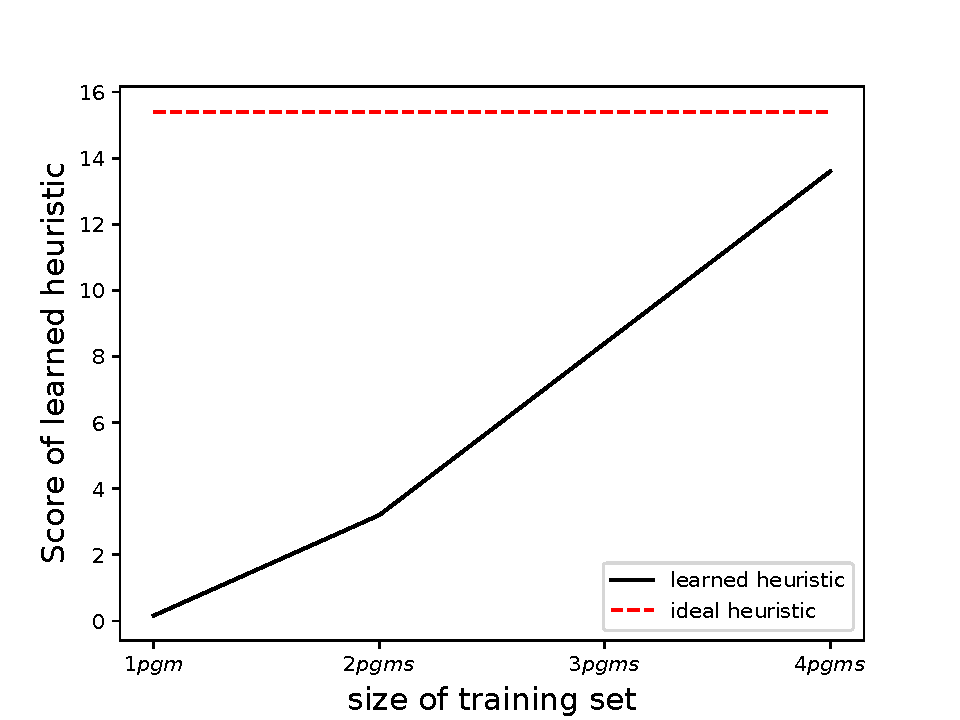
\includegraphics[width=7cm]{figures/training_set.pdf}
%	\caption{How score of learned heuristic changes over the value
%		of $\hyper$.}
%	\label{fig:training}
%\end{figure}


% Please add the following required packages to your document preamble:
% \usepackage{booktabs}
\begin{table}[]
\setlength\extrarowheight{-1pt}
\caption{Performance comparison among heuristics learned from various combinations of training sets (i.e. \onepgm, \twopgm, \threepgm, and \fourpgm) and an ideal heuristic (\ideal) against the validation program findbugs. \#proven casts presents the number of casts proved to be safe; a more precise analysis produces a larger number of \#proven casts.
The row score presents the quality of the heuristics computed by
${\mbox{\#proven casts}}\over{\mbox{analysis time (s)}}$.}
\label{tbl:training}
%${\projproved(F_P(\heuristic(G)))}\over{\projcost(F_P(\heuristic(G)))}$.}
\centering\scriptsize
\begin{tabular}{@{}lrrrrr@{}}
\toprule
%\multicolumn{1}{c}{} & \multicolumn{1}{c}{\onepgm} & \multicolumn{1}{c}{\twopgm} & \multicolumn{1}{c}{\threepgm} & \multicolumn{1}{c}{\fourpgm} & \multicolumn{1}{c}{\multirow{3}{*}{\ideal}} \\
\multicolumn{1}{c}{\multirow{2}{*}{}} & \multirow{2}{*}{\{luindex\}} & \multicolumn{1}{c}{\multirow{2}{*}{\{luindex, lusearch\}}} & \multicolumn{1}{c}{\{luindex, lusearch} & \multicolumn{1}{c}{\{luindex, lusearch} & \multicolumn{1}{c}{\multirow{2}{*}{\qquad\ideal}} \\
\multicolumn{1}{c}{} &  &  & \multicolumn{1}{c}{antlr\}}  & \multicolumn{1}{c}{antlr, pmd\}} &  \\ \midrule
analysis time (s)    & 4,090(+185)                                & 411(+107)                                  & 153(+226)                                    & 96(+363)                                    & 92                        \\
\#proven casts     & 672                                      & 1,321                                      & 1,289                                        & 1,315                                       & 1418                      \\ \midrule
score                & 0.16                   & 3.2                    & 8.4                      & 13.6                    & 15.4 \\\bottomrule
\end{tabular}
\end{table}


%\begin{figure}
%\vspace{-22pt}
%\begin{multicols}{2}
%~\\~\\~\\
%\begin{subfigure}[]{0.9\columnwidth}
%\small
%%\begin{tabular}{@{}c|lrr@{}}
%%\toprule
%%\multicolumn{1}{c}{}                          & \multicolumn{1}{c}{} & \multicolumn{1}{c}{\onepgm}   & \multicolumn{1}{c}{\twopgm}  \\ \midrule
%%\multirow{5}{*}{findbugs} & analysis time (s)    & 4,090(+185)                  & 411(+107)                   \\
%%                          & \#may-fail casts     & 2,417                        & 1,768                       \\ \cmidrule(){2-4}
%% & \multicolumn{1}{c}{} & \multicolumn{1}{c}{\threepgm} & \multicolumn{1}{c}{\fourpgm} \\
%%						  \cmidrule(){2-4}
%%                          & analysis time (s)    & 153(+226)                    & 96(+363)                    \\
%%                          & \#may-fail casts     & 1,800                        & 1,774                      \\\bottomrule
%%\end{tabular}
%\end{subfigure}
%
%\columnbreak
%\vspace{-57pt}
%\begin{subfigure}[t]{0.9\columnwidth}
%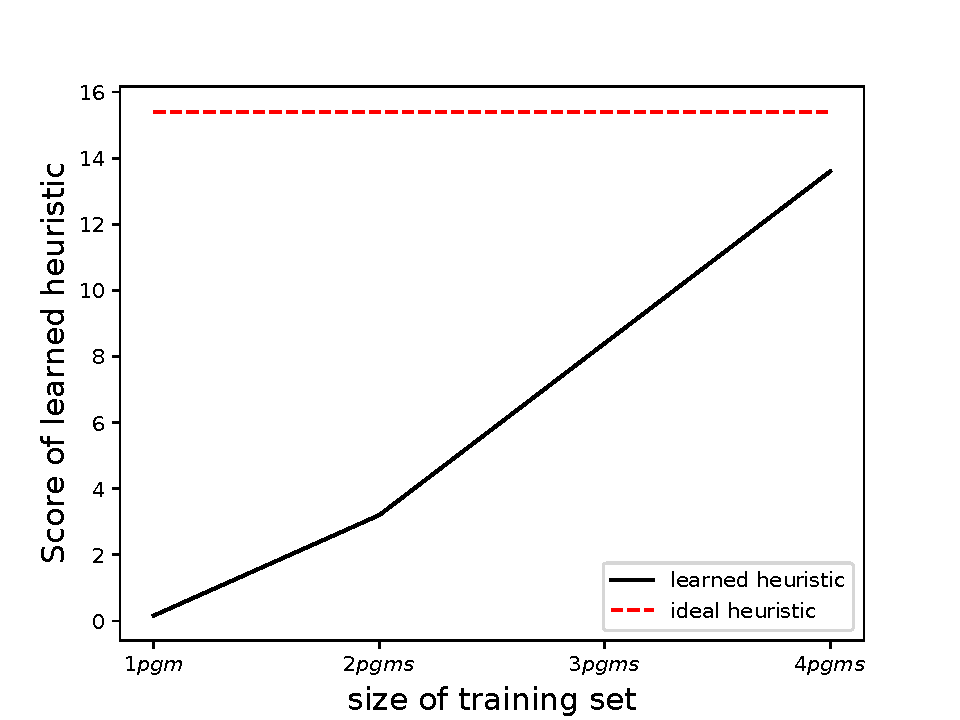
\includegraphics[width=7cm]{figures/training_set.pdf}
%\end{subfigure}
%\end{multicols}
%\vspace{-0.5cm}
%\caption{Performance of heuristics learned with various numbers (1$\sim$4) of training programs, and how score of learned heuristic changes over the size of training set.}
%\label{fig:training}
%\end{figure}

%
%	\centering
%	\begin{tabular}{cc}
%		% Please add the following required packages to your document preamble:
%% \usepackage{booktabs}
%% \usepackage{multirow}
%
%&
%		
%	\end{tabular}
%		of $\hyper$.}
%	\label{fig:gamma}
%






%%% Local Variables:
%%% mode: latex
%%% TeX-master: "paper"
%%% End: 
% !TEX root = ./paper.tex

%\textcolor{red}{
%The heuristics produced by \ourtool~ may not be general when the downstream clients for training steps are substantially different from those in evaluation.
%In experiments, we trained heuristics with the may-fail-cast client and evaluated the learned heuristics on the test set using three clients (may-fail-casts, poly-call-sites, and call-graph-edges).
%The evaluation results show that the heuristics learned by \ourtool~ are general in our evaluation environment.
%The performance, however, may be unsatisfactory if the clients in the main analysis are different from the ones used when training. In such a case, \ourtool~should be retrained with the new target client.
%}




\subsection{Limitations and Discussion}
%\TODO{Explain more about the limitation: e.g., Limitation 1 is ... Limitation 2 is ... And then discuss how to mitigate them in a separate paragraph.}
\ourtool~has several limitations.
One major limitation is that the heuristics produced by our approach may not be generalized
if the setting in training steps is substantially different from that used in evaluation in terms of analyzer $F$, target client, and $\CallDepth$.
More specifically, the learned heuristics by \ourtool~are dependent on the training data, the analyzer $F$ used, and the target client
(e.g., may-fail casts).
For example, the precision on the number of may-fail casts can be unsatisfactory if we train the heuristics with
the number of poly-call sites as the target client.
The context-length $\CallDepth$ for the main analysis is also limited to the one used in the training phase.
%d) the context-length k used in the training phase is rather limited.
Besides those generality issues, the training process of \ourtool~is time-consuming (i.e. it took 200 hours in our evaluation).

%As the heuristics produced by \ourtool~is learned with the a) the training data and b) specific analyzer $F$,
%the performance of \ourtool~may be unsatisfactory if the analyzer for main analysis is different from the one used in training phase.
%Similarly, using different clients for the main analysis from the training process can result in the degraded performance of \ourtool~
%in terms of precision and scalability.
%For example, the precision on the number of may-fail casts can be unsatisfactory if we train the heuristics with
%the number of poly-call sites as the target client.
%Further, e) the learning cost of~\ourtool takes about 200 hours for a single heuristic,
%which seems to be costly.

Despite those limitations, we believe \ourtool~can be useful in practice. %for other settings as well in practice.
First of all, note that in this paper we showed the effectiveness of \ourtool~in a realistic (yet particular) setting, where we used a real-world pointer analysis framework and benchmarks.
In particular, we do not believe the expensive training phase of \ourtool~is a serious limitation in practice, because it is not only fully automatic but also rather cheap compared to the much more expensive process of handcrafting analysis heuristics or features by human experts.
%\ourtool~can automate the manual process that typically requires weeks or months to develop a single heuristic.
%All the processes of generating the heuristics are fully automated, which can dramatically reduce the
%burdens of analysis designers in practice.
%Even with the limitations above,~\ourtool, however, can be still used realistically in a production setting.
%For example, although it takes about 200 hours to learn a single heuristic, it is cheaper than the manual process of
%designing cost-effective heuristics from the given graph, which typically takes weeks or months.
%Moreover, all the processes of generating the heuristics are fully automated, which can dramatically reduce the
%burdens of human-involving tasks.
The learned heuristic is dependent on the training data but, as we showed in this paper (Section~\ref{sec:justify}), using a small number of real programs is likely to provide a sufficient amount of actual training data (e.g., allocation sites) in practice. Also, the selection of training programs did not require careful engineering efforts in our case.
The context length $\CallDepth$ is rather limited (2-object-sensitivity), but 2-object-sensitive pointer analysis is generally considered to be highly precise in practice~\cite{Li2018a}.

For the issue on target clients, we showed that training heuristics using the may-fail-cast client
generalizes well for the three clients (may-fail-casts, poly-call-sites, and call-graph-edges).
When the downstream clients are substantially different, however,
one solution is to choose the target clients as general as possible in the training process. For example, we can use the size of context-insensitive variable points-to sets instead of the number of may-fail-casts as the context-insensitive variable points-to set is one of the most general clients that affect the others.
The clients we used in our evaluation (i.e. may-fail-casts, poly-call-sites, and call-graph-edges) are computed based on the context-insensitive variable points-to set and therefore minimizing it would likely minimize other clients too.
%
%\TODO{What is the point of the next paragraph? Saying another limitation and how to mitigate it? Be more explicit. }
%Despite its dependency on the settings (e.g., training data, analyzer $F$, target client, and context depth $k$) and learning cost,
%\ourtool~can be practically used in industry because user-involving tasks (e.g., deciding suitable settings) are light weighted and other processes are done automatically.
%More precisely, for the analyzer $F$, the users only need to decide the one among the other available analyzers to suit their tastes.
%Users can also organize the training data with other programs which have commonalities to the object program (e.g., functional behavior, type of inputs). These commonalities would likely provide appropriate data for learning.
%For the context depth $k$, the users can simply determine the highest context depth $k$
%by checking whether $\vec{k}$ (assign $k$ to all the program components) is scalable over the training programs while $\vec{k+1}$ (assign $k+1$ to all the program components) is not.
%With the selected settings above, \ourtool~automatically produces the cost-effective heuristics,
%of which the learning process takes about 200 hours.
%Although the learning cost seems to be expensive, we believe that it is reasonably cheaper compared to the cost of manually designing graph-based heuristics which additionally requires high expertise and lots of human effort.
%
%





%As \ourtool~automates the processes which typically require lots of human effort,
%it can reduce the burdens
%it is much more light weighted compared to manually designing graph-based heuristics which additionally requires high expertise and lots of human effort.

%Only with small effort on deciding the settings, \ourtool~automatically produces the cost-effective heuristics.







%\textcolor{blue}{Tone down the claim of Graphick as "an approach to learn heuristics for "object-sensitive" pointer analysis" instead of "a general-purpose approach to context-sensitive pointer analysis". In particular, argue convincingly how GraphicK can be used realistically in a production setting, given that (a) its training phase is time-consuming, (b) the learned predictor is dependent on the training data and the analyser F used, and (3) the context-length k used in the training phase is rather limited.}



%%% Local Variables:
%%% mode: latex
%%% TeX-master: "paper"
%%% End:

%\chapter{Related Work}\label{sec:Related}
%% !TEX root = ./paper.tex

\section{Conclusion and Future Work}

Unfortunately, the program analysis community for object-oriented programs has dismissed call-site sensitivity for a long time. 
In this paper, 
showed that 
call-site sensitivity has vast untapped potential, even more than object sensitivity, when the notion of $k$-limiting is generalized. We provided an insight that call-site sensitivity with context tunneling can simulate object sensitivity and experimentally proved that the observation holds in practice by developing a technique to transform a baseline object-sensitive analysis into more precise, context-tunneled call-site sensitivity. 
Based on our results, we hope that the community reconsiders call-site sensitivity from now on.  


%We demonstrated that our technique enables call-site sensitivity to outperform modern object-sensitive analyses for real-world Java programs in both precision and cost.

%when designing context-sensitive analyses.


Many problems remain as future work. We already discussed a theoretical issue in Section~\ref{sec:counter_example}. 
Other problems include the following. 


\begin{itemize}

\item {\em Can we learn better tunneling strategies than just simulating object sensitivity?} 
Our goal in this paper was to show that call-site sensitivity can be superior to object sensitivity, and simulating object sensitivity was an effective means of achieving this goal. 
However, simulating object sensitivity would be a suboptimal strategy for call-site sensitivity; 
we believe an optimal tunneling strategy would enable call-site sensitivity to show far better precision than ours (\ours).
Thus, an interesting direction for future work is to develop a powerful learning algorithm to find such strategies, where 
the main challenge is how to efficiently explore the huge and non-monotone tunneling space~\cite{JeJeOh18}. Using reinforcement learning, for example, could be a promising approach to address this challenge. 

%in the huge and non-monotone tunneling space~\cite{JeJeOh18}. 
%For example, reinforcement learning could be a promising approach to address this challenge.

\item {\em Can our approach be adapted for other flavors of context-sensitive analyses?}
Our current simulation technique relies on properties specific to $k$-CFA (e.g., $I_2$ in Section~\ref{sec:simulation} leverages a unique property of context-tunneled $k$-CFA). However, the high-level idea (i.e., simulating object sensitivity) would be applicable to other analyses. 
For example, it would be interesting if our idea could be adapted for $m$-CFA~\cite{Might10}. 
% by leveraging properties of context-tunneled $m$-CFA. 



% instead of k-CFA with your technique would produce better, similar, or worse results.


% High-level idea of our approach (simulating object sensitivity) is applicable to other contexts. 
%Directly applying our technique may not effective as
%it relies on specific properties of k-CFA (e.g., $I_2$ leverages a unique property of context-tunneled k-CFA).
%However, the high-level idea of our approach could be adapted.
%For example, applying our approach could be adapted for m-CFA~\cite{Might10} by leveraging properties of context tunneled m-CFA.

\end{itemize}






% \myparagraph{Future Work}

% \begin{itemize}

% \item {\bf Better context tunneling for call-site-sensitivity}:

% \item {\bf General technique for simulation}:  Our simulation technique was designed to work on the
%   call-graph produced by an object-sensitive analysis. Therefore, the
%   resulting call-site-sensitive analysis is likely to be effective for
%   type-dependent clients (e.g. may-fail casts).

%\end{itemize}

%%% Local Variables:
%%% mode: latex
%%% TeX-master: "paper"
%%% End:

\chapter{Related Work}\label{sec:Related}
% !TEX root = ./paper.tex

\section{Conclusion and Future Work}

Unfortunately, the program analysis community for object-oriented programs has dismissed call-site sensitivity for a long time. 
In this paper, 
showed that 
call-site sensitivity has vast untapped potential, even more than object sensitivity, when the notion of $k$-limiting is generalized. We provided an insight that call-site sensitivity with context tunneling can simulate object sensitivity and experimentally proved that the observation holds in practice by developing a technique to transform a baseline object-sensitive analysis into more precise, context-tunneled call-site sensitivity. 
Based on our results, we hope that the community reconsiders call-site sensitivity from now on.  


%We demonstrated that our technique enables call-site sensitivity to outperform modern object-sensitive analyses for real-world Java programs in both precision and cost.

%when designing context-sensitive analyses.


Many problems remain as future work. We already discussed a theoretical issue in Section~\ref{sec:counter_example}. 
Other problems include the following. 


\begin{itemize}

\item {\em Can we learn better tunneling strategies than just simulating object sensitivity?} 
Our goal in this paper was to show that call-site sensitivity can be superior to object sensitivity, and simulating object sensitivity was an effective means of achieving this goal. 
However, simulating object sensitivity would be a suboptimal strategy for call-site sensitivity; 
we believe an optimal tunneling strategy would enable call-site sensitivity to show far better precision than ours (\ours).
Thus, an interesting direction for future work is to develop a powerful learning algorithm to find such strategies, where 
the main challenge is how to efficiently explore the huge and non-monotone tunneling space~\cite{JeJeOh18}. Using reinforcement learning, for example, could be a promising approach to address this challenge. 

%in the huge and non-monotone tunneling space~\cite{JeJeOh18}. 
%For example, reinforcement learning could be a promising approach to address this challenge.

\item {\em Can our approach be adapted for other flavors of context-sensitive analyses?}
Our current simulation technique relies on properties specific to $k$-CFA (e.g., $I_2$ in Section~\ref{sec:simulation} leverages a unique property of context-tunneled $k$-CFA). However, the high-level idea (i.e., simulating object sensitivity) would be applicable to other analyses. 
For example, it would be interesting if our idea could be adapted for $m$-CFA~\cite{Might10}. 
% by leveraging properties of context-tunneled $m$-CFA. 



% instead of k-CFA with your technique would produce better, similar, or worse results.


% High-level idea of our approach (simulating object sensitivity) is applicable to other contexts. 
%Directly applying our technique may not effective as
%it relies on specific properties of k-CFA (e.g., $I_2$ leverages a unique property of context-tunneled k-CFA).
%However, the high-level idea of our approach could be adapted.
%For example, applying our approach could be adapted for m-CFA~\cite{Might10} by leveraging properties of context tunneled m-CFA.

\end{itemize}






% \myparagraph{Future Work}

% \begin{itemize}

% \item {\bf Better context tunneling for call-site-sensitivity}:

% \item {\bf General technique for simulation}:  Our simulation technique was designed to work on the
%   call-graph produced by an object-sensitive analysis. Therefore, the
%   resulting call-site-sensitive analysis is likely to be effective for
%   type-dependent clients (e.g. may-fail casts).

%\end{itemize}

%%% Local Variables:
%%% mode: latex
%%% TeX-master: "paper"
%%% End:


\appendix
% !TEX root = ../thesis.tex

\chapter{Is Complete Simulation Possible?}\label{sec:appendix}
% In this thesis, we showed that it is practically possible to outperform object sensitivity via context-tunneled call-site sensitivity (Chapter~\ref{sec:Obj2CFA}). 
% However, it remains to be seen whether or not call-site sensitivity can be fundamentally superior to object sensitivity.
Before we introduce the formal description the fundamental superiority, we redefine pointer analysis with tunneling on which the formal description will be simply defined. Note that the analysis below is fundamentally the same with the analysis described in Chapter~\ref{sec:Preliminaries} and \ref{sec:Obj2CFA}.

%In this section, we define a pointer analysis with context tunneling. 


%\subsection{Context-Tunneled Pointer Analysis}
\label{sec:pointeranalysis}


\myparagraph{Program}
We assume a program is a sequence of instructions, where each
instruction is associated with a distinct label.  An instruction is
either heap allocation (${\it x = new()}$), move (${\it x = y}$), 
%\textcolor{red}{
store (${\it x.f = y}$), load (${\it x = y.f}$),
%}
or
virtual method call (${\it x = y.m_r^{p}(a)}$).  We
assume that every method ($m$) has a single formal parameter ($p$) and
return variable ($r$). 
Given a program $P$ to analyze, we assume the following:
\begin{itemize}[leftmargin=1.4em]
\item $\Var_P$: the set of program variables.
\item $\fld_P$: the set of field signatures.
\item $\Inst_P$: the set of instruction labels of the program.
\item $\Methods_P$: the set of methods of the program.
\item $\mthdof_P$: the mapping from labels to the
methods containing them (i.e. $\Inst_P \to \Methods_P$).
\item $\Invo_P$: invocation sites (i.e. call sites, $\Invo_P \subseteq \Inst_P$).
\item $\Heap_P$: heap allocation sites (i.e. $\Heap_P \subseteq \Inst_P$).
\item $\Ctx_P$: the set of calling contexts (i.e. $\Ctx_P = \Inst_P^*$).
\item $\Hctx_P$: the set of heap contexts (i.e. $\Hctx_P = \Inst_P^*$).
\item $\entry_P$: the entry method of the program.
\end{itemize}


\myparagraph{Notation}
For function $X: A \to B$, where $A$ and $B$ are sets, we write $X[a
\mapsto b]$ %\begin{comment}
(where $a \in A, b \in B$)
%\end{comment}
for the function $X$ that is extended to map  $a$ to $b$.
For function $X: A \to \power{B}$,
$X[ a \weakupdate b]$ 
%\begin{comment}
(where $a \in A, b \subseteq B$)
%\end{comment} 
denotes $X[ a\mapsto X(a) \cup b]$ (i.e. weak update).
Given $X, Y: A \to \power{B}$, $X \sqcup Y$ denotes $\lambda
a. X(a) \cup Y(a)$. Given a sequence $s = a_1a_2\dots a_{n-1}$ and an element
$a_n$, we write $\truncateCtx{s \concat a_n}{k}$ for $a_1a_2\dots a_{n-1}a_n$
if $n < k$. If $n \ge k$, the result is $a_{n-k+1} \dots a_{n-1}a_n$.


%\myparagraph{Tunneling Abstraction}
\myparagraph{Pointer Analysis} % with Context Tunneling}
%The idea of context tunneling~\cite{JeJeOh18} is to selectively update contexts. 
%To support context tunneling, we parameterize a pointer analysis by a tunneling abstraction, $T$, which is a set of invocation sites.  
%
%\begin{comment}
%For example, when
%$k=1$,  a caller method $m_{1}$ with context
%$[i_{1}]$ calls a method $m_{2}$ at call-site $i_{2}$, and
%$i_2 \in T$, the context of the callee $m_2$ inherits the caller's
%and becomes $[i_{1}]$, not $[i_{2}]$.  
%
%When $T =
%\emptyset$, we do not apply context tunneling at all, so the analysis
%becomes the conventional
%$k$-context-sensitive analysis. % that keeps the last
%% $k$ context elements.
%When $T =
%\Invo_P$, on the other hand, the analysis becomes context-insensitive
%because every call-site is tunneled and therefore all the
%methods are analyzed under the initial context of the entry method.
%%\end{comment}
%
%
%
%\myparagraph{Analysis Rules} 
We consider a subset-based pointer analysis with on-the-fly call-graph construction~\cite{Smaragdakis2015}, which computes four pieces of
information: points-to, field points-to, reachability, and call-graph
information. The points-to information,
$\ptsto\in \Var_P \times \Ctx_P \to \power{\Heap_P \times \Hctx_P}$, maps
variables with contexts to sets of heaps with heap contexts.  
The field points-to information,
$\fptsto \in \Heap_P \times \Hctx_P \times \fld_P \to \power{\Heap_P \times \Hctx_P}$, maps
fields of heaps with their heap contexts to sets of heaps with heap contexts.  
The
reachability information, $\reachable \in \Methods \to \power{\Ctx}$,
maps methods to their reachable contexts. 
A call-graph,
$\callgraph\in \power{\Invo_P \times \Ctx_P\times \Methods_P\times \Ctx_P}$,
is a set of context-sensitive call edges, where
$(\invo,\ctx_1,m,\ctx_2) \in \callgraph$ indicates that method $m$ is
called from the invocation-site $\invo$ and the caller and callee
contexts are $\ctx_1$ and $\ctx_2$, respectively. The analysis is
flow-insensitive and aims to compute the least fixed point of the semantic function $F$ defined as follows:
\[
F^{T,U}_{P,k} = \lambda (\ptsto, \fptsto, \reachable, \callgraph). \bigsqcup_{\inst \in \Inst_P}
f^{T, U}_{\inst, k}(\ptsto, \fptsto ,\reachable, \callgraph) 
\]
where $k \in \mbn$ is the maximum context depth to distinguish and  $f^{T, U}_{\inst, k}$ is the transfer function for the instruction whose label is $\inst$. $T$ and $U$ are context-tunneling abstraction and context-update function, respectively, which will be explained shortly. Running the analysis is to compute $\fix F$:
\[
\fix F^{T,U}_{P,k} = F^{T,U}_{P,k} (\bot_X, \bot_Y, \bot_R, \bot_G) \sqcup F^{T,U}_{P,k} (F^{T,U}_{P,k} (\bot_X, \bot_Y, \bot_R, \bot_G)) \sqcup \dots
\]
where the bottom elements are defined as follows:
\[
  \bot_\ptsto = \lambda (x,c).\emptyset, \qquad   \bot_\fptsto = \lambda (l,hc,f).\emptyset, \qquad \bot_\reachable =
\lambda m. \left\{ \begin{array}{ll} \myset{\epsilon} & \mbox{if}~m =
                                                        \entry_P \\
                     \emptyset & \mbox{otherwise} \end{array} \right., \qquad
  \bot_\callgraph = \emptyset.
\]


\myparagraph{Transfer Function}
The transfer function for the allocation, move, store, and load instructions is standard.
Let $(\ptsto', \fptsto', \reachable',\callgraph')$ be $f^{T, U}_{\inst, k}(\ptsto, \fptsto,\reachable,\callgraph)$. 
When the command is allocation ({\it x
  = new()}), it extends the points-to map so that the variable {\it x}
points-to the heap $\inst$ under the reachable context $\ctx \in \reachable(\mthdof(l))$: 
\[
\vspace{-0.3em}
%\begin{array}{c}
\ptsto' = \bigsqcup_{\ctx \in \reachable(\mthdof(l))} \ptsto [ (x,
\ctx)\weakupdate \myset{(l, \ctx)} ].
%\end{array}
\]
For a store command 
({\it ${\it x.f = y}$}), the field points-to information is updated as follows:
\[
\vspace{-0.3em}
%\begin{array}{c}
\fptsto' = \bigsqcup_{\ctx \in \reachable(\mthdof(l))} \fptsto [(l,
\hctx,f)\weakupdate \myset{(l', \hctx')} ]
%\end{array}
\]
where $(l,hctx) \in \ptsto(x,ctx)$ and $(l',\hctx') \in
X(y,\ctx)$. The points-to information is updated as follows for a
load (${\it x = y.f}$) instruction: 
\[
\vspace{-0.3em}
%\begin{array}{c}
\ptsto' = \bigsqcup_{\ctx \in \reachable(\mthdof(l))} \ptsto [(x,
\ctx)\weakupdate \myset{(l, \hctx)}]
%\end{array}
\]
where $(l,\hctx) \in \fptsto(l',\hctx',f)$ and $(l',\hctx') \in X(y,\ctx)$.
The reachability map and call-graph remain the same for the above instructions (i.e. $\reachable'=\reachable$ and $\callgraph'=\callgraph$). 
The transfer function for move instruction ($\it x = y$) combines the points-to set of
${\it y}$ into that of ${\it x}$ without modifying $\reachable$ and $\callgraph$.
%\[
%\ptsto' = \bigsqcup_{\ctx \in \reachable(\mthdof(l))} \ptsto[(x, \ctx) \weakupdate \ptsto(y,
%                 \ctx)].
%\]

The transfer function for method calls is less standard as it should 
account for context tunneling. 
To support context tunneling~\cite{JeJeOh18}, we assume a context-tunneling space $\mbs$ is given. 
The space $\mbs$ can be defined in various ways and the choice does not affect the soundness of the analysis. 
In this chapter, we simply define the space to be the set of all invocation sites, i.e., $\mbs = \Invo_P$ and let $T \subseteq \mbs$ be a tunneling abstraction given before the analysis. 
For method call ${\it x =
y.m^p_r(a)}$, 
the transfer function, $f^{T, U}_{\inst, k}$,  first generates the callee's context $\ctx'$ using the context-update function $\updatectx$, $\ctx' = \updatectx(\ctx, T, X, l, y, k)$, which takes information available at the
call-site. 
The output $\ctx'$ of $\updatectx$ will be shortly defined for each context sensitivity flavor.
Once $\ctx'$ is computed, the analysis makes the formal
parameter $p$ under $\ctx'$ have the points-to set of the actual
parameter $a$ under $\ctx$ and the points-to set of the return variable
$r$ is transferred to the variable
$x$. The resulting $\ptsto'$ is
defined as follows: 
\[
 \bigsqcup_{\ctx \in \reachable(\mthdof(l))}
  	\ptsto[	(p,\ctx')
	\weakupdate \ptsto(a, \ctx), 
	(x, \ctx) \weakupdate \ptsto(r,
	\ctx')]
\]
     and the reachability and call-graph are updated accordingly:
      $\reachable' = \reachable[ m \weakupdate \myset{\ctx'}]$ and $\callgraph' = \callgraph \cup\{(\inst,ctx,m,ctx')\}$.


%the analysis generate
%callee method's context and weak updates 

%When the instruction at $\inst$ is ${\it x =
%y.m^p_r(a)}$, $f_{k,i}^{T,
%\updatectx}(\ptsto,\reachable, \callgraph)$ takes care of parameter and return
%value passing, producing the following:
%\[
%\begin{array}{rr}
%\bigsqcup\limits_{\ctx \in \reachable(\mthdof(l))}
%\myset{(
%\ptsto
%\left[
%\begin{array}{l}
%             (p,\ctx')
%  \weakupdate \ptsto(a, \ctx), \\
%  (x, \ctx) \weakupdate \ptsto(r,
%  \ctx')
%\end{array}
%  \right], \reachable[ m \weakupdate \myset{\ctx'}],
%  \\\callgraph \cup\{(\inst,ctx,m,ctx')\})
%  \mid \ctx'=\updatectx^{k, T}(\ctx, X, l, y)}.
%\end{array}
%\]
%From the context $\ctx$, we first generate the callee's context
%$\ctx'$ using $\updatectx$, which takes information available at the
%call-site and produces new contexts (details to be explained shortly). Then, the analysis makes the formal
%parameter $p$ under $\ctx'$ have the points-to set of the actual
%parameter $a$ under $\ctx$. The points-to set of the return variable
%$r$ is transferred to the variable $x$. 
%%\end{itemize}

%\subsection{Context Tunneling}\label{sec:tunneling}
%
%We now define object sensitivity and call-site sensitivity with context tunneling. 

\myparagraph{Context Update}
Let us define the context-update function $\updatectx$. 
For object sensitivity, it is defined as follows: 
\begin{equation}\label{eq:objsens}
\begin{array}{rr}
\updatectx (\ctx, T, X, l, y, k) =
\left\{
\begin{array}{ll}
\truncateCtx{\hctx \concat h}{k} & l \not\in T, \\
\hctx & l \in T
\end{array}
\right.\\
\end{array}
\end{equation}
where $(h, \hctx) \in X(y, \ctx)$.
When a method is called from an
      invocation site $l$ with the base variable $y$ and caller's
      context $\ctx$, the analysis first looks at the heap $h$ (and
      its context $\hctx$) that the variable $y$ under $\ctx$ points
      to, and creates the callee's context by appending the heap ($h$)
      to its heap context ($\hctx$). The context may be truncated to
      keep the last $k$ elements at most (i.e.
      $\truncateCtx{\hctx \concat h}{k}$).
Note that 
$\updatectx$ creates the new context only when $l \not\in
T$ (i.e. no context tunneling). Otherwise ($l \in T$), it applies context tunneling and propagates the existing 
context ($\hctx$). 

%By combining the information, 
%The definition of $\updatectx$ for object-sensitivity~\cite{Milanova2005,Smaragdakis2011}
%is defined as follows:
% produces the callee's context.
%For instance, object-sensitivity~\cite{Milanova2005,Smaragdakis2011} can be specified
%by defining $\updatectx$ as follows:
%

%\paragraph{Call-Site Sensitivity}
For call-site sensitivity, $\updatectx$ is defined as follows: 
\begin{equation}\label{eq:cfa}
\updatectx(\ctx, T, X, l, y, k) =
    \left\{
      \begin{array}{ll}
        \truncateCtx{\ctx \concat l}{k} & l \not\in T, \\
        \ctx & l \in T
      \end{array}
    \right.
\end{equation}
When $l \not\in T$, 
%When a method is called at an invocation site $l$ in a method under the context
%$\ctx$, 
the analysis appends 
the current invocation site $l$ to
$\ctx$. With context tunneling ($l \in T$), it uses the caller's context $\ctx$ for the callee's. 



%\textcolor{red}{
%Note that we can define the abstraction space of context tunneling in various ways.
%In this paper, we use the set of invocation sites as an abstraction space; a tunneling abstraction determines whether to update contexts with method invocation sites. 
%In the previous work~\cite{JeJeOh18}, on the other hand, the space of tunneling is defined with methods; a tunneling abstraction determines whether to apply tunneling with methods.
%}

% \myparagraph{Instance Analyses}
% Given  a program $P$ and 
% its tunneling abstraction $T \subseteq \Invo_P$, 
% we write $\call_k(P, T)$ and
% $\obj_k(P, T)$ for the $k$-call-site- and
% $k$-object-sensitive analyses, respectively. In the rest of the paper, we fix $k$ and omit the subscript $k$ from $\call_k$ and $\obj_k$. 
% These instance analyses are used with a {\em context-tunneling policy}. 
% A context-tunneling policy $\heuristic$ is a function that maps a program $P$ into
% a tunneling abstraction for $P$: 
% \[
%   \heuristic(P) \subseteq \Invo_P.
% \]
% With a policy $\heuristic$, 
% we  perform the analysis for a program $P$ as follows: $\call(P, \heuristic(P))$ or $\obj(P, \heuristic(P))$. 

 % which first uses $\heuristic$ to produce a tunneling abstraction $\heuristic(P)$ and analyzes the program with the abstraction. 

%%% Local Variables:
%%% mode: latex
%%% TeX-master: "../thesis"
%%% End:

% !TEX root = ./paper.tex
\newcolumntype{Y}{>{\centering\arraybackslash}X}
%\setcopyright{none}
%\usepackage {tikz}
\usetikzlibrary {shapes,positioning}
%\usepackage {bm}
\tikzstyle{block} = [rectangle, draw, fill=white, text width=3.8em,
, text
centered, rounded corners, minimum height=4em]
\tikzstyle{block2} =
[rectangle, draw, fill=white, text width=6em, text centered, rounded
corners, minimum height=4em, minimum width = 7em] \tikzstyle{line} = [draw, -latex']
\tikzstyle{onlyText} = [text width =2em, text centered]
%\setcopyright{rightsretained}

\tikzstyle{block3} =
[rectangle, draw, fill=white, text width=7em, text centered, rounded
corners, minimum height=3em] \tikzstyle{line} = [draw, -latex']

%\setcopyright{rightsretained}


\tikzstyle{blocks} = [rectangle, draw, fill=white, text width=0.7cm, text height = 4em, text
centered,  text width=4em, rounded corners, minimum height=0.6cm]

% \chapter{Open Question: Is Complete Simulation Possible?}\label{sec:counter_example}

% In this paper, we showed that it is practically possible to outperform object sensitivity via context-tunneled call-site sensitivity. 
% %, which supports our claim that call-site sensitivity is empirically superior to object sensitivity in a more general $k$-limited setting. 
% However, it remains to be seen whether or not call-site sensitivity can be fundamentally superior to object sensitivity. 

\myparagraph{Fundamental superiority}Let us define the notion of `superiority' as follows: 
\begin{definition}[Superiority of Call-Site Sensitivity]
Let $\mbp$ be a set of target programs. Let $\mbs$ be a context-tunneling space for the target programs. 
We say call-site sensitivity is superior to object sensitivity with respect to $\mbs$ if 
is always possible to simulate object sensitivity via call-site sensitivity: 
\begin{equation}\label{eq:sup-condition}
\forall P \in \mbp. \forall T_{\it obj} \in \mbs.  \exists T_{\it call} \in \mbs.\forall k \in [0,\infty]. 
\; 
\fix F^{T_{\it call}, U_{\it call}}_{P, k} \moreprecise~\mbox{(more precise than)}~
\fix F^{T_{\it obj}, U_{\it obj}}_{P, k}
%\call_k(P, T_{\it call})~\mbox{is more precise than}~\obj_k(P, T_{\it obj}).
\end{equation}
where $U_{\it call}$ and $U_{\it obj}$ are context-update functions (Eq.~(\ref{eq:objsens}) and (\ref{eq:cfa})) that are naturally given together with the tunneling space $\mbs$, and the precision order $\moreprecise$ is defined in terms of the context-insensitive points-to sets, as follows: 
 \[
   \fix F_{P,k}^{T, \updatectx} \moreprecise \fix
   F_{P,k}^{T', \updatectx'} \iff \forall x\in \Var_P.\; \project(\fix
   F_{P,k}^{T, \updatectx})(x) \subseteq \project(\fix
   F_{P,k}^{T', \updatectx'}) (x)
 \]
where $\project(X, Y, R,\callgraph) = \lambda x.\; \bigsqcup_{\ctx \in \Ctx}
 \myset{h \mid (h, \hctx) \in X(x, \ctx)}$.
\end{definition}
Then, the question is restated as follows: Is there a context-tunneling space $\mbs$ that makes the condition (\ref{eq:sup-condition}) true? 

%Formally answering the question would be challenging, although we conjecture that the answer might be true. Let us explain why with examples.




\myparagraph{Object Sensitivity is Not Fundamentally Superior}
We first show that object sensitivity is not fundamentally superior to call-site sensitivity. 
That is, it is not possible to find a tunneling
abstraction space $\mbs$ that makes $k$-object sensitivity with
tunneling always equal or more precise than $k$-call-site
sensitivity with tunneling. The example code in
Figure~\ref{background:example2} is a universal counter-example for all 
tunneling spaces $\mbs$. By definition of context tunneling
(i.e., selective update of contexts), the method
{\tt id} in the example (Figure~\ref{background:example2}) can have
 \texttt{[D]} (updating context) or \texttt{[$\cdot$]}
(inheriting context) as a context no matter what tunneling abstraction space is
used. Thus, $k$-object sensitivity with tunneling is unable to separate the
three method calls (invoked at the three different invocation sites)
with the two 
available context choices. In summary, we conclude that object sensitivity cannot simulate call-site sensitivity even in the generalized setting with context tunneling. 

%k-call-site sensitivity, however, can separate the
%three method calls with a tunneling abstraction $\emptyset \subseteq
%S$ (always update contexts) for all tunneling abstraction space
%$S$ of context tunneling. 



\myparagraph{The Case for Call-Site Sensitivity}
On the other hand, the situation for call-site sensitivity is nontrivial and it remains to be seen whether or not call-site sensitivity can simulate object sensitivity completely. 
%we conjecture that call-site sensitivity can be fundamentally superior to object sensitivity with a well-designed context tunneling space. 
Let us explain in more detail with examples.



\begin{figure}[t]
\begin{multicols}{2}
%\vfill\null
~\\\\\\\\
\begin{subfigure}[b]{1.2\columnwidth}
\begin{lstlisting}[xleftmargin=13pt,multicols=2,basicstyle={\fontsize{8.5}{10}\selectfont\ttfamily}]
class C {
 C f;
 void m(C v) {
  this.set(v);
  v.set(this);
 }
 void set(C v) {
  this.f = v;
 }
}
void main() {
 C c1 = new C();//C1
 C c2 = new C();//C2

 c1.m(c2);
 c2.m(c1);
 assert(c1.f != c2.f); 
}
\end{lstlisting}
\caption{Example code}
\label{fig:counterexample:code}
\end{subfigure}
\columnbreak~\\


\quad\begin{subfigure}[b]{1.0\columnwidth}
\begin{center}
	\resizebox{0.55\columnwidth}{!}{
		\begin{tikzpicture}
		\tikzstyle{every node}=[font=\LARGE]
		\node [block] (main) {{\tt main} \\ $[\cdot]$};
		\node [block, above right = -0.4cm and
		0.7cm of main] (Dm1) {\tt {m} \\$[$C1$]$};
		\node [block, below = 0.4cm of Dm1] (Dm2) {\tt{m} \\$[$C2$]$};
		\node [block, right = 0.9cm of Dm1] (Cm1) {\tt {set} \\$[$C1$]$};
		\node [block, right = 0.9cm of Dm2] (Cm2) {\tt {set} \\$[$C2$]$};
		
		\path [line] (main) edge node[above] {$15$} (Dm1);
		\path [line] (main) edge node[above] {$16$} (Dm2);
		\path [line] (Dm1) edge node[above] {$4$} (Cm1);
		\path [line] (Dm2) edge node[below] {$4$} (Cm2);
		\path [line] (Dm2) edge node[above] {$5$} (Cm1);
		\path [line] (Dm1) edge node[below] {$5$} (Cm2);
		
		\end{tikzpicture}
	}
\end{center}
\caption{Call-graph by 1-object sensitivity}
\label{fig:counterexample:obj}
\end{subfigure}~\\



\quad\begin{subfigure}[b]{1.0\columnwidth}

\begin{center}
	\resizebox{0.55\columnwidth}{!}{
		\begin{tikzpicture}
		\tikzstyle{every node}=[font=\LARGE]   
		\node [block] (main) {{\tt main} \\ $[\cdot]$};
		\node [block, above right = -0.4cm and
		0.7cm of main] (Dm1) {{\tt m} \\$[15]$};
		\node [block, below = 0.4cm of Dm1] (Dm2) {{\tt m} \\$[16]$};
		\node [block, right = 0.9cm of Dm1] (Cm1) {{\tt set} \\$[4]$};
		\node [block, right = 0.9cm of Dm2] (Cm2) {{\tt set} \\$[5]$};
		
		\path [line] (main) edge node[above] {$15$} (Dm1);
		\path [line] (main) edge node[above] {$16$} (Dm2);
		\path [line] (Dm1) edge node[above] {$4$} (Cm1);
		\path [line] (Dm2) edge node[below] {$5$} (Cm2);
		\path [line] (Dm2) edge node[above left= 0.15cm and 0.02cm] {$5$} (Cm1);
		\path [line] (Dm1) edge node[below left= 0.15cm and 0.02cm] {$4$} (Cm2);	
		\end{tikzpicture}
	}
\end{center}
\caption{Call-graph by 1-call-site sensitivity}
\label{fig:counterexample:call}
\end{subfigure}

\end{multicols}
\vspace{-15pt}
\caption{Example such that call-site sensitivity cannot
  simulate object sensitivity w.r.t. tunneling space $\mbs = \Invo$.}
\vspace{-10pt}
\label{fig:counterexample}
\end{figure}

First, we point out that the condition (\ref{eq:sup-condition}) does not hold w.r.t. the tunneling space considered in this chapter. 
In Section~\ref{sec:setting}, we defined the tunneling space $\mbs$ to be the set of invocation-sites, i.e., $\mbs = \Invo$. 
With this space, there exists a tricky counter-example program that context-tunneled
call-site sensitivity is unable to simulate object sensitivity.
Consider the program in Figure~\ref{fig:counterexample}. 
In the example code, class {\tt C} contains two methods, {\tt set} and {\tt m}.
Method {\tt set} is a setter that stores the parameter value in the
the field of the base object,
and method {\tt m} calls the {\tt set} method twice
with the receiver object and parameter being swapped.
The {\tt main} method creates two objects, {\tt C1} and {\tt C2}, and
stores them in {\tt c1} and {\tt c2}. Method {\tt m} is called on {\tt
  c1} with parameter {\tt c2} at line 15, and it is called again on
{\tt c2} with parameter {\tt c1} at line 16.
At line 17, an assertion asks if
the fields of {\tt c1} and {\tt c2} are not aliased.
In the real execution, the query holds because {\tt c1.f} points to {\tt C2} and
{\tt c2.f} points to {\tt C1}.

The conventional 1-object-sensitive analysis can prove the query but
1-call-site sensitivity cannot do so no matter what tunneling abstraction from the space $\mbs = \Invo$ is
chosen.
Figure~\ref{fig:counterexample:obj} presents
the call-graph of 1-object sensitivity.
The object-sensitive analysis is effectively producing the call-graph above as
each context of {\tt set} determines the value of each parameter.
When the context is {\tt [C1]}, the receiver object is {\tt C1} and the value of the parameter is {\tt C2}.
Otherwise, when the context is {\tt [C2]}, the receiver object and the
parameter value are  {\tt C2} and {\tt C1}, respectively.
On the other hand, conventional 1-call-site sensitivity constructs a similar but
different call-graph in Figure~\ref{fig:counterexample:call}.
Note that the two edges labeled 4 go
to the same method but they are heading to different methods in the call-graph of object sensitivity. 
Thus, it is not possible to simulate object sensitivity with the invocation-site-based context tunneling. 
%However,
%doing so still fails to simulate object sensitivity.


%The code pattern, however, is uncommon in practice.
%To make call-site sensitivity unable to simulate object sensitivity,
%the program should have at least two invocation-sites where a single method
%is called with different parameters and receiver objects.
%The parameters should come from the parameters of the caller methods, and the
%caller method should be called from at least two different invocations with
%different parameters. Satisfying all of these constraints at the same time
%would happen rarely in practice.


%\textcolor{red}{
%\footnote{
%We can define the tunneling abstraction in various ways.
%\citet{JeJeOh18} originally used (pairs of) methods as tunneling abstractions.
%In this paper, we consider more fine-grained program elements, i.e., invocation-sites. 
%} 

\begin{figure}[t]
	\begin{center}
			\resizebox{0.8\columnwidth}{!}{
					\begin{tikzpicture}
					\tikzstyle{every node}=[font=\LARGE]
					\node [block] (main) {{\tt main} \\ $[\cdot]$};
					\node [block, right =
					2.0cm of main] (Dm1) {{\tt m} \\$[15]$};
					\node [block, left = 1.9cm of main] (Dm2) {{\tt m} \\$[16]$};
					\node [block, below right = -0.3cm and 1.9cm of Dm1] (Cm1) {{\tt set} \\$[5]$};
					\node [block, below left = -0.3cm and 1.9cm of Dm2] (Cm2) {{\tt set} \\$[4]$};
	
					\node [block, above = 0.4cm of Cm1] (Cm3) {{\tt set} \\$[15]$};
					\node [block, above = 0.4cm of Cm2] (Cm4) {{\tt set} \\$[16]$};
	
	
					\path [line] (main) edge node[above= 0.15cm] {\large$(C1,15)$} (Dm1);
					\path [line] (main) edge node[above= 0.15cm] {\large$(C2,16)$} (Dm2);
					\path [line] (Dm1) edge node[above left= 0.15cm and -0.7cm] {\large $(C1,4)$} (Cm3);
					\path [line] (Dm2) edge node[above right= 0.15cm and -0.7cm] {\large $(C1,5)$} (Cm4);
					\path [line] (Dm2) edge node[below right = 0.15cm and -0.7cm] {\large $(C2,4)$} (Cm2);
					\path [line] (Dm1) edge node[below left = 0.15cm and -0.7cm] {\large $(C2,5)$} (Cm1);
					\end{tikzpicture}
			}
	\end{center}
	\caption{Call-graph with a fine-grained tunneling space}
	\label{fig:cg-finegrained}
	\vspace{-10pt}
	\end{figure}
However, this counter-example does not mean that it is fundamentally impossible to simulate object sensitivity via call-site sensitivity, as the counter-example becomes no longer valid if we use a more fine-grained tunneling abstraction. 
For example, suppose we define the tunneling space to be pairs of receiver objects and invocation-sites, i.e., $\mbs = \Heap \times \Invo$ (recall that choosing a tunneling abstraction does not affect the analysis soundness). 
With this tunneling space, a context-tunneled 1-call-site-sensitive analysis can now prove the query. 
Suppose we use a tunneling abstraction $T = \myset{(C1,4), (C1,5)}$, which means that we apply context tunneling only when the receiver object is $C1$ and the invocation-site is either $4$ or $5$. 1-call-site sensitivity with $T$ produces the call-graph in Figure~\ref{fig:cg-finegrained}. 
In the call-graph, $\texttt{m[15]} \stackrel{(C1,4)}{\to}
\texttt{set[15]}$ indicates that the caller ({\tt m}) and callee ({\tt
  set}) have the same context 15 where the callee method is called at
invocation-site 4 and its receiver object is $C1$. With this call-graph, we can prove the query 
in Figure~\ref{fig:counterexample:code} as it is strictly more precise than the call-graph produced by object sensitivity
(Figure~\ref{fig:counterexample:obj}). 



%Note that the above counter-example is not valid that 1-call-site
%sensitivity with tunneling can prove the query if we use a generalized
%abstraction space of context tunneling instead of invocation sites. if
%we use pairs of receiver objects and invocation sites as tunneling
%abstraction, 1-call-site-sensitive analysis with tunneling can prove
%the query in the example
%(Figure~\ref{fig:counterexample:call}). Suppose we use a
%tunneling abstraction $T = \{(C1,4),(C1,5)\}$ where it applied context
%tunneling when the receiver object and invocation site are $C1$ and
%$4$, respectively, or the object and the invocation site are $C2$
%and $5$, respectively. It produces
%the following context abstraction:



This way, we conjecture that it would be always possible to find a suitable context-tunneling space $\mbs$ that satisfies the condition (\ref{eq:sup-condition}) w.r.t. the given set of programs ($\mbp$). We leave an in-depth theoretical analysis as future work. 

%}




%%% Local Variables:
%%% mode: latex
%%% TeX-master: "paper"
%%% End:

%


%the high-level idea of our approach could be adapted for m-CFA and we think it will be an interesting direction for extending our work.
%Our current simulation technique relies on specific properties of k-CFA (e.g., I_2I 2​	
%leverages a unique property of context-tunneled k-CFA). Therefore applying our technique as it is may not be effective for m-CFA [2]. 

%\section{Notations}\label{sec:max}
%The function $\MaxIn(G_\vec{P})$ returns the maximum number $max\in\mbn$ of
%incoming edges of a node in the graphs that $max$ satisfies:
%%\[
%%\begin{array}{c}
%\begin{enumerate}
%\item %There exists a node $n$ that have $max$ incoming edges:\\
%$max$ is a node's incoming edges:
%$\exists P\in\vec{P}. (N,E) =
%  G_\vec{P}(P) \land \exists n\in N. |\{n' \mid (n',n)\in E\}| = max$
%\item The node has equal or more number of
%incomingedges than the others: \\
%$\forall P \in \vec{P}. (N,E) = G_\vec{P}(P) \land \forall n\in N. |\{n' \mid (n',n)\in E
%\}| \le max$
%\end{enumerate}
%%\end{array}
%%\]
%On the other hand, $\MaxOut(G_\vec{P})$ returns the maximum number $max\in\mbn$ of
%outgoing edge of a node in the graphs:
%\begin{enumerate}
%\item $max$ is a node's outgoing edges: $\exists P\in\vec{P}. (N,E) = G_\vec{P}(P) \land \exists n\in N. |\{n' \mid (n,n')\in E
%\}| = max$
%\item The node has equal or more number of
%incomingedges than the others: \\
%$\forall P \in \vec{P}. (N,E) = G_\vec{P}(P) \land \forall n\in N. |\{n' \mid (n,n')\in E
%\}| \le max$
%\end{enumerate}

% \[
% Incoming(n,G) = |\{n' \mid (n',n)\in E \land G = (N,E) \}|
% \]
% \[
% Outgoing(n,G) = |\{n' \mid (n,n')\in E \land G = (N,E) \}|
% \]
% \[
% \forall n \in G' \in G_\vec{P}. Incoming(n,G) \ge Incoming(n',G')
% \]
% where $Incoming$ returns the number of incoming edges for each node:
% \[
% Incoming(n,G) = |\{n' \mid (n',n)\in E \land G = (N,E) \}|
% \]
% On the other hand, $\MaxOut(G_\vec{P})$ returns the maximul number of incoming edges
% of a node $n$ in the graphs:
% \[
% \forall n \in G_\vec{P}. Incoming(n,G) \ge Incoming(n',G')
% \]
% where $Outgoing$ returns the number of the node's outgoing edges:
% \[
% Outgoing(n,G) = |\{n' \mid (n,n')\in E \land G = (N,E) \}|
% \]



\chapter{Proof of Theorem~\ref{THM:REDUCESPACE}}\label{sec:proof}

%{\textsc LearningMinimalAbstraction}\label{alg:Learnminimal}

We will show that the output of Algorithm~\ref{alg:Learnminimal} in Section~\ref{sec:learning-algorithm} is the minimal abstraction of the given program using proof by induction and contradiction.
Let $\abs$ be the output of the learning algorithm.  
$\abs$ is a precise abstraction because our algorithm updates $\abs$ only if the following equation holds:
\[
\projproved(F_P(\abs)) = \projproved(F_P(\absk)).
\]
Assume that $\abs'$ meets the precision constraint but smaller than $\abs$:
\begin{equation}\label{eq:assumption}
\projproved(F_P(\abs')) = \projproved(F_P(\absk)) \land
\abs' \sqsubseteq \abs.
\end{equation}
We can prove that $\abs$ is the minimal abstraction by showing that $\abs'$ equals to $\abs$:
%It suffices to show that:
\begin{equation}\label{eq:goal}
\forall i \in [0,k].\{c \mid c \in \component_P \land \abs(c) = i\} = \{c \mid c\in \component_P \land \abs'(c) = i\}.
\end{equation}
We prove~(\ref{eq:goal}) with induction on $i$ in decreasing order.
\begin{itemize}
\item (Base case) the base case is as follows:
\begin{equation}\label{eq:base:goal}
\{c \mid c\in \component_P \land \abs(c) = k\} = \{c \mid c\in \component_P \land \abs'(c) = k\}.
\end{equation}
From~(\ref{eq:assumption}), we have
\begin{equation}\label{eq:base:obvious}
\emptyset = \{c \mid c\in \component_P \land \abs'(c) = k\} \setminus \{c \mid c\in \component_P \land \abs(c) = k\}.
\end{equation}
Now, we can prove~(\ref{eq:base:goal}) by showing the following counterpart is also $\emptyset$ by the proof of contradiction:
\begin{equation}\label{eq:base:counter}
\{c \mid c\in \component_P \land \abs(c) = k\} \setminus \{c \mid c\in \component_P \land \abs'(c) = k\}.
\end{equation}
Assume that~(\ref{eq:base:counter}) is not an empty set, then it has a program component $c'$:
\[
c' \in (\{c \mid c\in \component_P \land \abs(c) = k\} \setminus \{c \mid c\in \component_P \land \abs'(c) = k\}).
\]
%Let $\abs''$ be the abstraction when $c'$ was considered in the first iteration.
Let $\abs''$ be the abstraction when $c'$ is chosen.
Then, we have
\begin{equation}\label{eq:base:small}
 \abs'\sqsubseteq \abs''.
\end{equation}
The abstraction $\abs''$ is less precise than $\vec{k}$:
%not precise enough as $c'$ is rejected:
\begin{equation}\label{eq:base:notprecise}
\projproved(F_P(\abs''))<\projproved(F_P(\absk)).
\end{equation}
From~(\ref{eq:assumption}),~(\ref{eq:base:small}), and the monotonicity of analysis, we have
\begin{equation}\label{eq:base:precise}
\projproved(F_P(\absk)) = \projproved(F_P(\abs')) \le \projproved(F_P(\abs'')).
\end{equation}
Now, we have a contradiction between~(\ref{eq:base:notprecise}) and~(\ref{eq:base:precise}).
As a result, we have:
\begin{equation}\label{eq:base:Notobvious}
\emptyset = (\{c \mid c\in \component_P \land \abs(c) = k\} \setminus \{c \mid c\in \component_P \land \abs'(c) = k\}).
\end{equation}
From~(\ref{eq:base:obvious}) and~(\ref{eq:base:Notobvious}), we prove the base case~(\ref{eq:base:goal}) is true.\\

\item (Inductive case) 
The induction hypothesis is as follows:
\begin{equation}\label{eq:ind:hypo}
\forall j \in [l,k].\{c \mid c \in \component_P \land \abs(c) = j\} = \{c \mid c \in \component_P \land \abs'(c) = j\}
\end{equation}
where $2\le l\le k$.
From the hypothesis, we will prove that the following equation is true:
\begin{equation}\label{eq:ind:goal}
\{c \mid c \in \component_P \land \abs(c) = l-1\} = \{c \mid c\in \component_P \land \abs'(c) = l-1\}.
\end{equation}
From~(\ref{eq:assumption}) and~(\ref{eq:ind:hypo}), we have
\begin{equation}\label{eq:ind:obvious}
\emptyset = \{c \mid c\in \component_P \land \abs'(c) = l-1\} \setminus \{c \mid c\in \component_P \land \abs(c) = l-1\}.
\end{equation}
Now, we will show the following counterpart is also $\emptyset$ by the proof of contradiction:
\begin{equation}\label{eq:ind:counter}
\{c \mid c\in \component_P \land \abs(c) = l-1\} \setminus \{c \mid c\in \component_P \land \abs'(c) = l-1\}.
\end{equation}
Assume that (\ref{eq:ind:counter}) has a program component $c''$.
Let $\abs'''$ be the abstraction when $c''$ is considered where $i$ equals to $l-1$ in the Algorithm~\ref{alg:Learnminimal}. From~(\ref{eq:ind:hypo}), we can get the following relation between $\abs'$ and $\abs'''$:
\begin{equation}\label{eq:ind:small}
\abs'\sqsubseteq \abs'''.
\end{equation}
$\abs'''$ is less precise than $\vec{k}$:
%not precise enough as $c'$ is rejected:
\begin{equation}\label{eq:ind:notprecise}
\projproved(F_P(\abs'''))<\projproved(F_P(\absk)).
\end{equation}
From~(\ref{eq:assumption}),~(\ref{eq:ind:small}), and the monotonicity of analysis, we have
\begin{equation}\label{eq:ind:precise}
\projproved(F_P(\absk)) = \projproved(F_P(\abs')) \le \projproved(F_P(\abs''')).
\end{equation}
We also find a contradiction between~(\ref{eq:ind:notprecise}) and~(\ref{eq:ind:precise}).
Now, we have
\begin{equation}\label{eq:ind:Notobvious}
\emptyset = (\{c \mid c\in \component_P \land \abs(c) = l-1\} \setminus \{c \mid c\in \component_P \land \abs'(c) = l-1\}).
\end{equation}
From~(\ref{eq:ind:obvious}) and~(\ref{eq:ind:Notobvious}), we can prove the following equation is true:
\[
\{c \mid c\in \component_P \land a_P(c) = l-1\} = \{c \mid c\in \component_P \land a_P'(c) = l-1\}.
\]

\end{itemize}


%%% Local Variables:
%%% mode: latex
%%% TeX-master: "paper"
%%% End:




%%%%%%%%%%%%%%%%%%%%%%%%%%%%%%%%%%%%%%%%%%%%%%%%%%%%
%                  여기까지 추가                   %
%%%%%%%%%%%%%%%%%%%%%%%%%%%%%%%%%%%%%%%%%%%%%%%%%%%%

\end{document}
